\documentclass[12pt]{thesul}

\usepackage{acronym} % Acronyms \ac[p], \acl[p], \acs[p], \acf[p]

\acrodef{CRDT}[CRDT]{Conflict-free Replicated Data Type}
\acrodefplural{CRDT}[CRDTs]{Conflict-free Replicated Data Types}

\acrodef{poset}[poset]{partially ordered set}

\acrodef{VTNS}[VTNS]{Visibilité Transitive Non-Spéculative}

\acrodef{FJC}[FJC]{Fork-Join-Causal}
\acrodef{VFJC}[VFJC]{View-\acl{FJC}}
\acrodef{SVFJC}[SVFJC]{Stabilizable-\acl{VFJC}}

\acrodef{BFT}[BFT]{Byzantine Fault-Tolerant}

\acrodef{CS}[CS]{Causal Stability}
\acrodef{PCS}[PCS]{Provable \acl{CS}}
\acrodef{VFJCS}[VFJCS]{\acl{VFJC} Stability}

\acrodef{fjc}[fjc]{fork-join-causally}
\acrodef{vfjc}[vfjc]{view-\acl{fjc}}

\acrodef{cs}[cs]{causalement stable}
\acrodefplural{cs}[cs]{causalement stables}
\acrodef{pcs}[pcs]{provably \acl{cs}}
\acrodef{vfjcs}[vfjcs]{\acl{vfjc} stable}

\acrodef{MUTE}[MUTE]{Multi-User Text Editor}

\acrodef{RGA}[RGA]{Replicated Growable Array}

%\usepackage{algorithm} % just for floats
\usepackage{algpseudocode} % algorithmicx default layout
% http://ctan.mines-albi.fr/macros/latex/exptl/biblatex/doc/biblatex.pdf
\usepackage{csquotes} % fix babel warning
\usepackage[
  defernumbers=true,
  sorting=none,
  maxbibnames=20,
  maxcitenames=1
]{biblatex}

\addbibresource{references/bft.bib}
\addbibresource{references/collaborative.bib}
\addbibresource{references/consistency.bib}
\addbibresource{references/crdt.bib}
\addbibresource{references/general.bib}
\addbibresource{references/math.bib}
\addbibresource{references/publications.bib}

\usepackage[draft,inline,nomargin,index]{fixme}
% theme = signature | coloring
\fxsetup{theme=signature,mode=multiuser,inlineface=\itshape,envface=\itshape}
\FXRegisterAuthor{fc}{afc}{François}
\FXRegisterAuthor{go}{ago}{Gerald}
\FXRegisterAuthor{mn}{amn}{Matthieu}
\FXRegisterAuthor{vic}{avic}{Vic.}

%
\usepackage{showframe}

\usepackage{graphicx}
\graphicspath{{./fig/}}

\usepackage[export]{adjustbox}
  % Enable use of graphic positioning
  % e.g. \includegraphics[right]{...}

\usepackage{subcaption}
\captionsetup{subrefformat=parens}

\usepackage[
  unicode=true,
  pdftitle={},
  pdfauthor={},
  pdfsubject={},
  pdfkeywords={},
  pdfstartview=Fit,
  bookmarks=false,
  hyperindex,
  colorlinks=true,
  linkcolor=black,
  citecolor=black,
  urlcolor=black
 ]{hyperref}

\newcommand{\propositionautorefname}{Proposition}

%\newcommand{\theoremautorefname}{Théorème}
\newcommand{\corollaryautorefname}{Corollaire}
\newcommand{\lemmaautorefname}{Lemme}
\newcommand{\claimautorefname}{Affirmation}

\newcommand{\definitionautorefname}{Définition}

% Remove warning about unset thesul bookmark level
% FIXME: should be integrated in the thesul class
% See https://tex.stackexchange.com/questions/123575/how-to-suppress-the-author-bookmark-generated-by-svmult-with-bookmark-package-wi
\makeatletter
\providecommand*{\toclevel@tulstarchapter}{0} 
\makeatother

% Theorem
\usepackage{amsthm}

\newtheorem{proposition}{Proposition}[chapter]

\newtheorem{claim}{Affirmation}[chapter]

\newtheorem{theorem}{Théorème}[chapter]
\newtheorem{corollary}{Corollaire}[theorem]
\newtheorem{lemma}{Lemme}[theorem]

\theoremstyle{definition}
\newtheorem{definition}{Definition}[chapter]

\theoremstyle{remark}
\newtheorem*{remark}{Remarque}

\newtheoremstyle{case}
  {}{} % Space above/below
  {\normalfont} % Body font
  {} % Indent amount
  {\itshape} % Theorem head font
  {.} % Punctuation after theorem head
  { } % Space after head, (' ', '\newline')
  {\thmname{#1}\thmnumber{ #2}\thmnote{ #3}}

\theoremstyle{case}
\newtheorem*{case}{Cas}

% Math
\usepackage{amsmath,amssymb}
\usepackage{mathtools} % fix amsmath bugs + better typeset

% Math - paired notations
% Each commands
% - has a * version that scales to the size of the content
%   e.g. set*{x}
% - an option to specify delimiter size
%   e.g. set[\Big]{x}
%   among: \big, \Big, \bigg, \Bigg

\DeclarePairedDelimiter{\card}{\lvert}{\rvert}

\DeclarePairedDelimiter{\tuple}{\langle}{\rangle}

\providecommand{\given{}}
\newcommand*{\setgivenpart}[1][]{%
    \nonscript\:#1\vert\allowbreak\nonscript\:\mathopen{}}
\DeclarePairedDelimiterX{\set}[1]{\{}{\}}{%
    \renewcommand\given{\setgivenpart[\delimsize]}#1}
\DeclarePairedDelimiterX{\setopen}[1]{\{}{.}{%
    \renewcommand\given{\setgivenpart[\delimsize]}#1}
\DeclarePairedDelimiterX{\setclose}[1]{.}{\}}{%
    \renewcommand\given{\setgivenpart[\delimsize]}#1}

% Math - other notations

\newcommand*{\lappend}{\operatorname{++}}
\newcommand*{\sminus}{-} % set minus
\newcommand*{\qsep}{\ldotp} % separator between quantifier and predicate
\newcommand*{\trm}[1]{\operatorname{\mathsf{#1}}} % custom math term
\newcommand*{\powerset}[1]{\mathcal{P} (#1)}
\newcommand*{\powerfset}[1]{\mathcal{P}_{\mathsf{fin}} (#1)}
\newcommand*{\defeq}{\overset{\mathrm{def}}{=}}
\newcommand*{\defiff}{\overset{\mathrm{def}}{\iff}}
\newcommand*{\assign}{\operatorname{\vcentcolon=}}
\newcommand{\irange}[2]{#1 \mathinner{\ldotp\ldotp} #2}
\newcommand*{\pto}{\hookrightarrow}
%\newcommand*{\pto}{\mathrel{\ooalign{\hfil$\mapstochar\mkern5mu$\hfil\cr$\to$\cr}}}

\newcommand*{\where}{\mathrel{\mathbf{where}}} % where keyword
\newcommand*{\when}{\mathrel{\mathbf{if}}} % if keyword

\newcommand*{\rb}{\overset{\mathsf{rb}}{\longrightarrow}} % returns-before
\newcommand*{\vis}{\overset{\mathsf{vis}}{\longrightarrow}} % visibility
\newcommand*{\viseq}{\leq_{\trm{vis}}} % visibility or equality
\newcommand*{\nviseq}{\nleq_{\trm{vis}}} % neither visibility nor equality
\newcommand*{\integr}{\overset{\mathsf{int}}{\longrightarrow}} % integration
\newcommand*{\concur}{\|} % concurrency
\newcommand*{\pre}{\longrightarrow} % precedence
\newcommand*{\idr}{\downarrow} % immediate dependency relation
\newcommand*{\dep}{\overset{\mathsf{dep}}{\longrightarrow}} % dep
\newcommand*{\ao}{\overset{\mathsf{ao}}{\longrightarrow}} % dep
\newcommand*{\hb}{\overset{\mathsf{hb}}{\longrightarrow}} % happens-before

% List
\usepackage[inline]{enumitem}
\setlist[description]{leftmargin=0cm}

\newlist{inlinelist}{enumerate*}{1}
\setlist*[inlinelist,1]{%
  label=(\roman*), % chktex 36
}

% Mini-tables
\usepackage[french]{minitoc}

% Named labels
\makeatletter % Enable to call macro with @
\newcommand*{\namedlabel}[2]{\begingroup
    #2%
    \def\@currentlabel{#2}%
    \phantomsection\label{#1}\endgroup
}
\makeatother % Disable @ as normal character

% Layout
\setlength{\HeadRuleWidth}{0.4pt}

% Warn against obsoletes
\usepackage[l2tabu, orthodox]{nag}

\usepackage{tikz}
\usetikzlibrary{arrows.meta} % '-latex' arrow
%\usetikzlibrary{backgrounds}
\usetikzlibrary{fit} % fit attribute
\usetikzlibrary{positioning}
\usetikzlibrary{shapes.misc} % rounded rectangle

%\usetikzlibrary{external}
%\tikzexternalize[prefix=tikz/]

\tikzset{
    com/.style = {dashed,-latex},
    link/.style = {dotted,line width=0.5mm},
    %timeline/.style = {dotted,line width=0.25mm,-{Latex[length=2.5mm,width=1.25mm]}},
    timeline/.style = {dotted,semithick},
    timedevt/.style= {shape=rounded rectangle,inner sep=0,fill=black,minimum height=0.1cm,anchor=west}
}

\tikzset{
    hb/.style = {-latex},
    vis/.style = {-latex},
    pre/.style = {-latex}
}

\tikzset{
    stable/.style = {draw}
}

\newcommand\widthletter{9mm}
\newcommand\widthblock{15mm}

\tikzset{
    common/.style={anchor=west, draw, rectangle, minimum height=\widthletter},
    letter/.style={common, minimum width=\widthletter},
    block/.style={common, minimum width=\widthblock},
    crossed/.style={
        path picture={
            \draw(path picture bounding box.south west)-- (path picture bounding box.north east);
        }
    }
}

%
% PLEASE DO NOT USE FOLLOWING ENVS
%

% Prefix every command with 'u' (u like user)

%\newenvironment{utikzhbgraph}{%
%    \tikzset{every label/.style={draw,fill=white,label distance=-1mm,text centered,text width={width ("vfjcs")},text height={height ("vfjcs")},inner sep=1mm}}
%    \tikzset{every pin/.style={pin distance=3mm}}
%    \tikzset{every pin edge/.style={{Circle}-}}
%
%    \tikzset{event/.style = {draw,shape=circle,fill=white,text width={width ("AAA")},align=center,inner sep=0}}
%    \tikzset{ulabel/.style = {draw,fill=white,text centered,text width={width ("vfjcs")},text height={height ("vfjcs")},inner sep=1mm}}
%    %% \uevent{node-id}{position}{content}
%
%    \newcommand{\uevent}[3]{\node[event] (##1) at (##2) {};\node[] at (##1) {##3};}%
%    \newcommand{\uevt}[3]{\node[event] (##1) at (##2) {##3};}%
%    %% \uhb{source}{target}
%    \newcommand{\uhb}[2]{\draw[hb] (##1) to (##2);}%
%    %% \ulabelled{labelled-node-id}{at-most-five-letter-label}
%    \newcommand{\ulabelled}[2]{%
%        \path (##1.south west) to +(0.2,0) node[ulabel,below left]{##2};%
%    }%
%    %% \uembedded{embedded-node-id}{relative-pos}{text}
%    %% relative-pos: below|above left|right
%    \newcommand{\uembedded}[3]{%
%        \node[##2=-7.5pt and -7.5pt of ##1] (uembeddedp0##1) {};%
%        \node[##2=10pt and 1pt of ##1] (uembeddedp1##1) {};%
%        \draw[-Circle] (uembeddedp1##1) to (uembeddedp0##1);%
%        \node[##2=-10pt and -7pt of uembeddedp1##1] {##3};}%
%    %% \uparticipants{event-node-id}{relative-pos}{coma-seperated-list-of-participants}
%    %% relative-pos: below|above left|right
%    \newcommand{\uparticipants}[3]{\uembedded{##1}{##2}{$\left\{##3\right\}$}}%
%    \begin{tikzpicture}%
%}{\end{tikzpicture}}
%
%\newcounter{timelinecount}
%%\utikzcomgraph[evt-spacing]{timeline-length}{timeline-spacing}
%\newenvironment{utikzcomgraph}[3][0.8]{%
%    \newcommand{\pevtspacing}{#1}
%    \newcommand{\ptimelinelen}{#2}
%    \newcommand{\ptimelinespacing}{#3}
%    \tikzset{evt/.style = {fill,circle,inner sep=0,minimum size=1.5mm}}
%    \tikzset{com/.style = {dashed,line width=0.25mm,-{Latex[length=2mm,width=2mm]}}}
%    \setcounter{timelinecount}{0}
%    \newcommand{\vtimelinecount}{\value{timelinecount}}
%    %% \utimeline{timeline-id}
%    \newcommand{\utimeline}[1]{%
%        \stepcounter{timelinecount};%
%        \node (##1) at (0,\vtimelinecount*\ptimelinespacing) {##1};%
%        \draw (##1) edge[timeline] ++(\ptimelinelen,0);%
%    }
%    %% \uanchor[label]{anchor-id}{utimeline-id}{tick}
%    \newcommand{\uanchor}[4][]{%
%        \path (##3) to ++(##4*\pevtspacing,0) node[inner sep=0](##2){};%
%        \path (##2) to ++(0,0.5) node{##1};%
%    }
%    %% \uevt{evt-id}{utimeline-id}{tick}{evt-label}
%    \newcommand{\uevt}[4]{%
%        \path (##2) to ++(##3*\pevtspacing,0) node[evt](##1){};%
%        \path (##1) to ++(0,0.5) node{##4};%
%    }
%    %% \usend{evt-id}{timeline-id}{tick}
%    \newcommand{\usend}[3]{%
%        \uanchor{##2rcv##1}{##2}{##3};%
%        \draw[com] (##1) to (##2rcv##1);%
%    }
%    \begin{tikzpicture}%
%}{\end{tikzpicture}}
%
%\newenvironment{utikzcollab}{%
%    % \udevice{device-id}{x,y}{display-name}
%    \newcommand{\udevice}[4][below]{%
%        \node[label=##1:{##4}] (##2) at (##3) {
\includegraphics[scale=0.4]{fig/utikzcollab/device.pdf}};%
%    }
%    % \ulink{src}{dest}
%    \newcommand{\ulink}[2]{%
%        \draw (##1) edge[link] (##2);%
%    }
%    \newcommand{\usync}[2]{%
%        \draw[link] (##1) -- (##2) node[midway]{
\includegraphics[scale=0.4]{fig/utikzcollab/sync.pdf}};%
%    }
%    % \udlabel{device-id}{orientation}{label-content}
%    % orientation = above left | above right | below left | below right
%    \newcommand{\udlabel}[3]{%
%        \edef\pos{##2}%
%        \edef\al{above left}%
%        \edef\ar{above right}%
%        \edef\bl{below left}%
%        \edef\br{below right}%
%        \ifx\pos\al%
%            \path (##1) to ++(-0.4,0) node[anchor=south east]{##3};%
%        \else\ifx\pos\ar%
%            \path (##1) to ++(0.4,0) node[anchor=south west]{##3};%
%        \else\ifx\pos\bl%
%            \path (##1) to ++(-0.4,0) node[anchor=north east]{##3};%
%        \else\ifx\pos\br%
%            \path (##1) to ++(0.4,0) node[anchor=north west]{##3};%
%        \else%
%            \PackageError{current}{invalid orientation}{}%
%        \fi\fi\fi\fi%
%    }
%    \begin{tikzpicture}%
%}{\end{tikzpicture}}
%
% http://www.khirevich.com/latex/microtype/
\usepackage[
    % enable chars to cross the margin
    activate={true,nocompatibility},
    % enable in draft mode
    final,
    tracking=true,
    kerning=true,
    spacing=true,
    factor=1100,
    % enable char stetching/shrinking 10 = 1%
    stretch=10,
    shrink=10]{microtype}
% reduce space between SmallCaps introduced by tracking=true
\SetTracking{encoding={*}, shape=sc}{40}

\usepackage{type1cm} % remove font size limit (for lettrines)
\usepackage{lettrine}

% remmove indent, add paragraph spacing
%\usepackage{parskip}


% TIP: You should also remove 'draft' from the class
%\ThesisDraft


% Which chapter to include?
\includeonly{
0-abstract,
1-intro,
2-problematic,
3-background,
5-auth-log,
6-delta-seq-crdt,
7-conclusion%,
%8-math-notations
}

%\tikzexternalize

\begin{document}
\ThesisTitle{Réplication sécurisée dans les infrastructures pair-à-pair de collaboration}
\ThesisDate{jour J}
\ThesisAuthor{Victorien Elvinger}
\ThesisUL{}
\ThesisDomain{mention informatique}
\AddLab{}
\President={À déterminer}
\Rapporteurs={
    Emmanuelle Anceaume & Directrice de recherche, IRISA\\
    Pascal Molli & Professeur des universités, Université de Nantes}
\Examinateurs={Esther Pacitti & Professeure des universités, Université de Montpellier 2\\
    Steve Kremer & Directeur de recherche, Inria Grand Est}
\Encadrants={François Charoy & Professeur des universités, Université de Lorraine\\
    Gérald oster & Maître de conférence, Université de Lorraine}
\MakeThesisTitlePage{}

\WriteChapterLabelInToc{}
\dominitoc{} % mini-toc init

\tableofcontents

\DontWriteThisInToc\listoffigures
\DontWriteThisInToc\listoftables
%\DontWriteThisInToc\listoftheorems[ignore={remark,lemma}]%

\mainmatter{}

\chapter{Introduction}

\minitoc{}
\bigskip

Ce premier chapitre introduit les infrastructures de collaboration. Il motive notre intérêt pour les infrastructures pair-à-pair de collaboration.
Il donne un aperçu de nos problématiques de recherche et de nos contributions.
Il détaille également l'organisation de ce manuscrit et il énumère nos publications.

\clearpage
\section{Contexte}

% Note : ne pas se centrer sur l'édition collaborative, mettre des exemples

%Internet est devenu une plate-forme où les utilisateur·ice·s et les services automatisés ne consultent plus uniquement des contenus, mais les produisent et les enrichissent collectivement.
%Les utilisateur·ice·s bénéficient de l'expérience de chacun·e.
%Les contenus produits sont plus élaborés et de meilleure qualité.
%
%Les applications de collaboration facilitent la production collaborative de contenus.
%Elles permettent à des collaborateur·ices géographiquement éloignés de contribuer à un même contenu.
%Elles permettent également de modifier simultanément ou de manière différée les contenus.
%Chaque contributeur·ice modifie individuellement un contenu partagé.
%Ses modifications sont à termes observées et prises en compte par les autres contributeur·ice·s.
%
%\begin{itemize}
%    \item Les éditeurs collaboratifs de texte permettent d'écrire en simultané.
%    \item Les réseaux sociaux permettent de partager et de commenter des contenus multimédias.
%\end{itemize}{}


%Les infrastructures de collaboration permettent à un groupe d'individus et de services automatisés de produire collectivement des contenus.

Internet est devenu une plate-forme où les internautes ne consultent plus uniquement des contenus, mais les produisent et les enrichissent collectivement~\autocite{mogan2010_web2groupware}~: elles et ils partagent et commentent des contenus multimédias au sein des réseaux sociaux~; elles et ils co-écrivent des documents à l'aide d'éditeurs collaboratifs~; elles et ils co-programment à l'aide de gestionnaires de versions.
Les productions de tels contenus sont le résultat d'activités de collaboration~\autocite{ellis1991_groupware} qui se répartissent dans l'espace et le temps.
Les contributeur·ices modifient individuellement un contenu partagé.
Elles et ils peuvent se trouver à des endroits géographiquement éloignés et peuvent modifier simultanément ou de manière différée les contenus partagés.
Leurs modifications sont à terme observées et prises en compte par les autres contributeur·ice·s.

% les systèmes centralisées

Les applications de collaboration ont permis l'émergence et la diffusion des activités de collaboration sur Internet.
Ces applications ont été initialement conçues sur des infrastructures centralisées.
Dans de telles infrastructures, les activités de collaboration s'organisent autour d'un serveur.
Les collaborateur·ice·s sont connecté·e·s les un·e·s aux autres à travers le serveur.
Toutes les modifications qu'elles et ils effectuent sur les contenus partagés sont relayées par le serveur aux autres collaborateur·ice·s.
Le serveur peut éventuellement transformer les modifications avant de les transmettre.
Dans la \autoref{fig:authority} les collaboratrices soumettent leur modification au serveur qui les appliquent sur le contenu.
Le serveur transmet la nouvelle version du contenu aux collaboratrices.
Le rôle prépondérant du serveur engendre plusieurs problèmes~:

\begin{figure}[hbt]
\centering
\begin{subfigure}{.5\linewidth}
    \centering
    \begin{tikzpicture}
        % devices
        \node[
            label=below:{Serveur}
        ](S){
\includegraphics[scale=0.8]{collab/cloud.pdf}};
        \path (S)
            to +(180:3.6) node[
                label=below:{Alice}
            ](A){
\includegraphics[scale=0.6]{collab/device.pdf}}
            to +(35:3.6) node[
                label=below:{Bea}
            ](B){
\includegraphics[scale=0.6]{collab/device.pdf}}
            to +(-35:3.6) node[
                label=below:{Carol}
            ](C){
\includegraphics[scale=0.6]{collab/device.pdf}};
        % Links
        \draw[link,-latex] (A) to node[near start]{
            
\includegraphics[scale=0.5]{collab/contrib-a1.pdf}
        } (S);
        \draw[link,-latex] (B.west) to node[near start]{
            
\includegraphics[scale=0.5]{collab/contrib-b1.pdf}
        } (S);
        \draw[link] (C.west) to (S);
    \end{tikzpicture}
    \caption{}\label{fig:authority-1}
\end{subfigure}%
\begin{subfigure}{.5\linewidth}
\centering
    \begin{tikzpicture}
        % devices
        \node[
            label=below:{Serveur}
        ](S){
\includegraphics[scale=0.8]{collab/cloud.pdf}};
        \path (S)
            to +(180:1.8) coordinate (Adoc)
            to +(180:3.6) node[
                label=below:{Alice}
            ](A){
\includegraphics[scale=0.6]{collab/device.pdf}}
            to +(35:1.8) coordinate (Bdoc)
            to +(35:3.6) node[
                label=below:{Bea}
            ](B){
\includegraphics[scale=0.6]{collab/device.pdf}}
            to +(330:1.8) coordinate (Cdoc)
            to +(-35:3.6) node[
                label=below:{Carol}
            ](C){
\includegraphics[scale=0.6]{collab/device.pdf}};
        % Links
        \draw[link,-latex] (S) to (A);
        \draw[link,-latex] (S) to (B.west);
        \draw[link,-latex] (S) to (C.west);
        % Msgs
        \node at (Adoc) {
\includegraphics[scale=0.5]{collab/doc-a1-b1.pdf}};
        \node at (Bdoc) {
\includegraphics[scale=0.5]{collab/doc-a1-b1.pdf}};
        \node at (Cdoc) {
\includegraphics[scale=0.5]{collab/doc-a1-b1.pdf}};
    \end{tikzpicture}
    \caption{}\label{fig:authority-2}
\end{subfigure}
\caption[Activité de collaboration au sein d'une infrastructure centralisée]{Exemple d'une activité de collaboration au sein d'une infrastructure centralisée.
Alice, Bea, et Carol sont connectées à un serveur.
Elles éditent ensemble un dessin.
\subref{fig:authority-1} Alice et Bea souhaitent modifier le dessin partagé~: Alice souhaite ajouter un carré et Bea souhaite ajouter un cercle.
Elles soumettent leur modification au serveur.
\subref{fig:authority-2} Le serveur intègre leurs modifications et transmet la nouvelle version du dessin aux collaboratrices.}\label{fig:authority}
\end{figure}

\paragraph{Disponibilité.}
Toutes les modifications du contenu partagé sont transmises aux collaborateur·ice·s par l'intermédiaire du serveur.
L'indisponibilité du serveur rend impossible la collaboration.
Le serveur est un \emph{point unique de défaillance}~\autocite{dooley2001designing}.

\paragraph{Latence.}
Le traitement centralisé des modifications effectuées par les collaborateur·ice·s introduit des latences.
Ces latences, ajoutées à celles du réseau, peuvent être trop importantes pour la modification de contenu en simultané.
Nous parlons de simultané quand des collaborateur·ice·s éditent un même contenu au même moment et qu'elles et ils ont l'illusion de percevoir immédiatement les modifications de chacun·e.
\textcite{ignat_2015_user-and-delay} ont montré que les activités de collaboration en simultané étaient compromises lorsque le délai entre des modifications de contenu et leurs observations par les autres était trop important.
Ce délai engendre des conflits de modification sur le contenu partagé.
Les collaborateur·ice·s adoptent des stratégies qui limitent leurs interactions pour éviter ces conflits.
Ce qui réduit l'efficacité de la collaboration.
%Les latences doivent être suffisamment faibles pour prendre en compte les modifications des autres collaborateur·ice·s lorsque nous effectuons nos propres modifications.

\paragraph{Passage à l'échelle.}
Le serveur peut difficilement s'adapter à un accroissement du nombre de modifications et du nombre de collaborateur·ice·s.
Cette difficulté se traduit par une augmentation des latences pour intégrer de nouvelles modifications et propager les nouvelles versions du contenu partagé.
Elle peut également produire un déni de service qui rend indisponible le serveur.
Pour éviter ce problème les applications de collaboration limitent le nombre de collaborateur·ice·s autorisé·e·s au sein d'une collaboration~\autocite{ignat_2015_user-and-delay,ignat2014_delayeffect}.
Ils supportent pas ou difficilement les activités de collaboration qui impliquent un nombre important de collaborateur·ice·s.

%\paragraph{Coût.}
%Afin de réduire les latences introduites par les infrastructures centralisées et de supporter un nombre raisonnable de collaborateur·ice·s, le serveur est en général dotée d'une puissance de calcul conséquente.
%Cette puissance de calcul engendre des coût environnementaux et financiers.
%Ce qui se traduit également par le contrôle de telles infrastructures par des organisations qui disposent des ressources nécessaires à leur déploiement.

\paragraph{Confidentialité, Vie Privée, et Censure.}
Le rôle de carrefour du serveur permet la collecte massive de données privées et confidentielles, ainsi que le contrôle systématique de l'information et donc de son éventuelle censure \autocite{jard2016_langage}.

\paragraph{Sécurité.}
Le rôle central du serveur en fait une cible privilégiée d'attaque \autocite{jard2016_langage}.
La corruption du serveur permet à l'attaquant d'accéder à de nombreuses données sensibles des utilisateur·ice·s et éventuellement de les altérer.

\paragraph{Propriété des contenus.}
Le serveur détient les contenus partagés.
Les collaborateur·ice·s perdent la propriété de leurs contenus et de leurs contributions.
Le serveur peut ainsi restreindre la modification et la consultation des contenus produits.
Il peut supprimer le contenu sans en alerter préalablement les contributeur·ice·s.

\paragraph{Modes de collaboration~\autocite{dourish_1995_divergence}.}
Les collaborateur·ice·s sont restreint·e·s dans les formes que peuvent prendre leur collaboration.
Les infrastructures centralisées leur permettent de contribuer depuis des endroits géographiquement éloignés et à des instants différents.
Toutefois elles et ils doivent être connecté·e·s au serveur.
Ils ne peuvent pas travailler en sous-groupes déconnecté·e·s les un·e·s des autres.
La modification hors ligne, voire la consultation hors ligne, des contenus partagés n'est pas toujours supportée.

\bigskip

%Son indisponibilité rend les collaborations impossibles.
%La serveur constitue donc un point unique de défaillance.
%Par ailleurs, les infrastructures centralisées passent difficilement à l'échelle.
%Elles peuvent souffrir de latence trop importante pour la modification de contenu en simultané.
%\textcite{ignat_2015_user-and-delay} ont en effet montré que les activités de collaboration en simultané étaient compromises lorsque le délai entre des modifications de contenu et leurs observations par les autres était trop important.
%
%Au-delà de leurs limitations techniques, les infrastructures centralisés soulèvent des questionnement éthiques.
%Le rôle de carrefour du serveur permet la collecte massive de données privées et confidentielles, ainsi que le contrôle systématique de l'information et donc de son éventuelle censure.
%Ces comportements peuvent être menés par l'organisation qui contrôle et maintient l'infrastructure ou par un attaquant.
%Se pose également la question de la propriété des contenus produits.

% les infrastructures pair-à-pair de collaboration

\begin{figure}[t]
\centering
\begin{subfigure}{.5\linewidth}
    \centering
    \begin{tikzpicture}
        % devices
        \path (0,0)
            to +(190:2) node[
                label=below:{Alice},
                label=left:{
\includegraphics[scale=0.5]{collab/doc-a1.pdf}}
            ](A){
\includegraphics[scale=0.6]{collab/device.pdf}}
            to +(70:2) node[
                label=above:{Bea},
                label=right:{
\includegraphics[scale=0.5]{collab/doc-b1.pdf}}
            ](B){
\includegraphics[scale=0.6]{collab/device.pdf}}
            to +(-50:2) node[
                label=below:{Carol},
                label=right:{
\includegraphics[scale=0.5]{collab/doc.pdf}}
            ](C){
\includegraphics[scale=0.6]{collab/device.pdf}};
        % Links
        \draw[link] (A) to (B);
        \draw[link] (B) to (C);
        \draw[link] (C) to (A);
    \end{tikzpicture}
    \caption{}\label{fig:optimisqtic-replciation-scenario-1}
\end{subfigure}%
\begin{subfigure}{.5\linewidth}
\centering
    \begin{tikzpicture}
        % devices
        \path (0,0)
            to +(190:2) node[
                label=below:{Alice},
                label=left:{
\includegraphics[scale=0.5]{collab/doc-a1-b1.pdf}}
            ](A){
\includegraphics[scale=0.6]{collab/device.pdf}}
            to +(70:2) node[
                label=above:{Bea},
                label=right:{
\includegraphics[scale=0.5]{collab/doc-a1-b1.pdf}}
            ](B){
\includegraphics[scale=0.6]{collab/device.pdf}}
            to +(-50:2) node[
                label=below:{Carol},
                label=right:{
\includegraphics[scale=0.5]{collab/doc-a1-b1.pdf}}
            ](C){
\includegraphics[scale=0.6]{collab/device.pdf}};
        % Links
        \draw[link] (A) to node[midway]{
\includegraphics[scale=0.5]{collab/sync.pdf}} (B);
        \draw[link] (B) to node[midway]{
\includegraphics[scale=0.5]{collab/sync.pdf}} (C);
        \draw[link] (C) to node[midway]{
\includegraphics[scale=0.5]{collab/sync.pdf}} (A);
    \end{tikzpicture}
    \caption{}\label{fig:optimisqtic-replciation-scenario-2}
\end{subfigure}
\caption[Activité de collaboration au sein d'une infrastructure pair-à-pair]{Exemple d'une activité de collaboration au sein d'une infrastructure pair-à-pair.
Alice, Bea, et Carol répliquent de manière optimiste un dessin.
Elles disposent chacune d'une copie du dessin.
\subref{fig:optimisqtic-replciation-scenario-1} Alice et Bea modifient indépendamment leur copie du dessin.
Alice ajoute un carré, alors que Bea ajoute un cercle.
Les copies des collaboratrices divergent~: les collaboratrices ont des dessins différents.
\subref{fig:optimisqtic-replciation-scenario-2} Elles synchronisent ensuite leurs copies afin d'intégrer les modifications de chacune.
Les copies convergent~: elles obtiennent ainsi le même dessin.}\label{fig:optimisqtic-replciation-scenario}
\end{figure}

La diffusion des activités de collaboration a inspiré de nouveaux usages qui poussent les infrastructures centralisées à leurs limites.
Par exemple, la prise de note en simultané durant un cours en ligne peut faire intervenir une promotion entière d'étudiant·e·s.
Ces usages se sont renforcés avec la crise sanitaire provoquée par la pandémie de \emph{COVID-19}.

Pour supporter ces nouveaux usages, plusieurs initiatives ont vu le jour~\autocite{benet2014ipfs,wood2014ethereum,mansour2016demonstration}.
Elles s'appuient sur des infrastructures pair-à-pair pour décentraliser les applications de collaboration.
Les infrastructures pair-à-pair de collaboration sont caractérisées par l'absence de serveur central.
Les appareils des collaborateur·ice·s sont des pairs.
Ils sont directement connectés les uns aux autres et partagent les mêmes responsabilités\footnote{Certaines infrastructures présentent des pairs privilégiés avec des responsabilités supplémentaires.%L'infrastructure reste décentralisée car plusieurs pairs peuvent avoir les mêmes privilèges.
}.

Les infrastructures pair-à-pair de collaboration visent la conception d'applications de collaboration hautement disponibles, aux latences faibles, qui tolèrent les partitions réseaux, et passent à l'échelle~\autocite{rodrigues2010peer}.
Pour ce faire, elles reposent sur la réplication optimiste des contenus~\autocite{saito_2005_optimisticreplication}.
Chaque pair possède une copie des contenus partagés.
Il interroge et modifie directement sa copie sans se coordonner avec les autres pairs.
Les modifications sont propagées en arrière plan aux autres pairs.
%Elles sont transmises immédiatement ou ultérieurement.
%Ce choix est laissé à la discrétion du protocole de réplication.
Les pairs intègrent à leur copie les modifications qu'ils reçoivent.
La \autoref{fig:optimisqtic-replciation-scenario} illustre un scénario de réplication optimiste.

%Le support de collaboration qui implique un grand nombre de collaborateur·ice·s augmente le risque d'apparition de latences et de comportements mal-intentionnés.
%Ce qui nous amène à questionner le passage à l'échelle et la sécurité des protocoles de réplication optimiste de contenu partagé.
%Nous détaillons ces aspects dans la \autoref{sec:problematic}.

Les infrastructures pair-à-pair de collaboration donne plus de responsabilités aux pairs.
Des collaborateur·ice·s peuvent davantage nuire au bon déroulement de la collaboration.
Les infrastructures pair-à-pair permettent également la participation d'un plus grand nombre de collaborateur·ice·s.
Ce qui nous amène à questionner la sécurité et le passage à l'échelle des protocoles de réplication optimiste.


\section{Problématiques et contributions}\label{sec:problematic}

%Les infrastructures pair-à-pair de collaboration permettent d'envisager la conception d'applications hautement disponible, aux latences faibles, et qui passent à l'échelle.

\subsection{Convergence en présence de pairs mal-intentionnés}

Les infrastructures pair-à-pair de collaboration permettent aux pairs de modifier en parallèle un contenu partagé.
Pour ce faire, les pairs répliquent le contenu partagé et modifient leur copie respective.
La modification concurrente du contenu engendre inévitablement la divergence des copies du contenu partagé~\autocite{dourish_1995_divergence}.
Dans la \autoref{fig:optimisqtic-replciation-scenario}, les copies divergent avant leur synchronisation.
Les protocoles de réplication optimiste sont responsables de la réconciliation de l'état des copies pour les faire converger vers un état qui intègre les modifications de chacun.
La convergence des copies conditionne la vivacité et donc le succès d'une collaboration.
Si deux contributeur·ice·s ont des copies qui ne sont pas capables de converger, leur vue du contenu sera différente.
Cette divergence de vue peut compromettre leur collaboration.
Assurer à terme la convergence des copies est donc important dans une infrastructure de collaboration.

Pour illustrer l'importance de la convergence, nous prenons l'exemple de l'organisation d'un événement festif ou politique.
Plusieurs réunions d'organisation ont lieu avant l'évènement.
Pour garder une trace de ces réunions et informer les bénévoles absents, les organisatrices de l'événement ont mis en place un document textuel partagé.
Les organisatrices et les bénévoles prennent collectivement des notes durant les réunions.
Ce document peut par exemple inclure des dates de rendez-vous pour préparer l'événement.
Si les pairs ne sont pas capables de converger, certains bénévoles risquent de manquer des rendez-vous essentiels.
Ce qui pourrait retarder, voire empêcher, la tenue de l'événement.

Certains pairs peuvent trouver un intérêt à compromettre le succès d'une collaboration.
Dans le cas de l'exemple précédent, il peut s'agir d'un opposant à la tenue de l'événement.
Nous nous intéressons en particulier aux pairs qui entreprennent des actions pour faire diverger de manière permanente la vue des autres pairs.
Ces pairs \emph{mal-intentionnés} cherchent donc à faire diverger de manière permanente les copies des autres pairs que nous qualifions d'\emph{honnêtes}.
Pour ce faire, les pairs mal-intentionnés utilisent les faiblesses de certains protocoles de réplication~: ils transmettent à différents pairs honnêtes des modifications distinctes qui sont perçues comme identiques par le protocole.
Il s'agit d'une \emph{équivoque}.
Par exemple, l'opposant à l'événement peut infiltrer le groupe de bénévoles et faire en sorte que les bénévoles observent différentes dates de rendez-vous de préparation de l'événement.
L'opposant répandrait ainsi la confusion et provoquerait l'absence de bénévoles à certains rendez-vous.
La \autoref{fig:equivocation-scenario} illustre un scénario dans lequel un pair mal-intentionné effectue une équivoque.
Les pairs honnêtes ne détectent pas l'équivoque.
Leurs copies divergent de manière permanente.

\paragraph{}Ce qui nous amène à formuler notre première question de recherche~: \textbf{Est-il possible d'assurer la convergence des copies des pairs honnêtes en présence de pairs mal-intentionnés et de conserver les propriétés offertes par les infrastructures pair-à-pair de collaboration~?}

\clearpage % better layout

\begin{figure}[hbt]
\centering
\begin{subfigure}{.5\linewidth}
    \centering
    \begin{tikzpicture}
        % devices
        \path (0,0)
            to +(190:2) node[
                label=below:{Alice},
                label=left:{
\includegraphics[scale=0.5]{collab/doc-a1-b1.pdf}}
            ](A){
\includegraphics[scale=0.6]{collab/device.pdf}}
            to +(70:2) node[
                label=above:{Bea},
                label=right:{
\includegraphics[scale=0.5]{collab/doc-a1-b1.pdf}}
            ](B){
\includegraphics[scale=0.6]{collab/device.pdf}}
            to +(-50:2) node[
                label=below:{Mallory}
            ](M){
\includegraphics[scale=0.6]{collab/device-malicious.pdf}};
        % Links
        \draw[link] (A) to (B);
        \draw[link,-latex] (M) to node[near start]{
\includegraphics[scale=0.5]{collab/contrib-m1.pdf}} (A);
        \draw[link,-latex] (M) to node[near start]{
\includegraphics[scale=0.5]{collab/contrib-m1p.pdf}} (B);
    \end{tikzpicture}
    \caption{}\label{fig:equivocation-scenario-1}
\end{subfigure}%
\begin{subfigure}{.5\linewidth}
\centering
    \begin{tikzpicture}
        % devices
        \path (0,0)
            to +(190:2) node[
                label=below:{Alice},
                label=left:{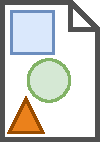
\includegraphics[scale=0.5]{collab/doc-a1-b1-m1.pdf}}
            ](A){
\includegraphics[scale=0.6]{collab/device.pdf}}
            to +(70:2) node[
                label=above:{Bea},
                label=right:{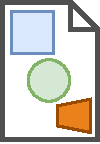
\includegraphics[scale=0.5]{collab/doc-a1-b1-m1p.pdf}}
            ](B){
\includegraphics[scale=0.6]{collab/device.pdf}}
            to +(-50:2) node[
                label=below:{Mallory}
            ](M){
\includegraphics[scale=0.6]{collab/device-malicious.pdf}};
        % Links
        \draw[link] (A) to node[midway]{
\includegraphics[scale=0.5]{collab/sync.pdf}} (B);
        \draw[link] (M) to (A);
        \draw[link] (M) to (B);
    \end{tikzpicture}
    \caption{}\label{fig:equivocation-scenario-2}
\end{subfigure}
\caption[Équivoque]{Exemple d'une équivoque qui vise à faire diverger de manière permanente les copies des collaboratrices honnêtes.
Alice et Bea sont honnêtes.
Elles répliquent de manière optimiste un dessin.
Mallory est mal-intentionnée.
Elle souhaite compromettre la collaboration entre Alice et Bea.
\subref{fig:equivocation-scenario-1} Mallory effectue une équivoque.
Elle transmet à Alice l'ajout d'un triangle orange, alors qu'elle transmet à Bea l'ajout d'un trapèze orange.
Elle fait en sorte que ces modifications distinctes paraissent identiques.
Par exemple, si l'on considère que la couleur est la seule information utilisée pour détecter la présence d'une forme sur le dessin, alors il n'est pas possible de différencier un dessin avec la première forme d'un dessin avec la seconde.
\subref{fig:equivocation-scenario-2} Alice et Bea intègrent la modification qu'elles reçoivent.
Leurs copies divergent.
Elles se synchronisent ensuite, mais elles ne détectent pas la divergence de leur copie.
L'objectif de Mallory est atteint~: les copies de Alice et Bea demeurent divergentes.}\label{fig:equivocation-scenario}
\end{figure}

De nombreux protocoles de réplication optimiste synchronisent les copies en échangeant des opérations~\autocite{baquero_2018_pure-op-crdt}.
L'opération synthétise une modification effectuée sur l'une des copies.
Un pair mal-intentionné met en œuvre une équivoque en générant deux opérations distinctes mais qui sont perçues comme identiques par le protocole de réplication.
Pour détecter de telles opérations, les pairs peuvent utiliser des \emph{journaux infalsifiables} d'opérations~\autocite{li_2004_sundr,mahajan_depot_2011,truong_authenticating_2012}.
Chaque pair possède un journal dans lequel il enregistre les opérations qu'il transmet et qu'il reçoit.
Chaque opération est signée par son auteur et référence des opérations sur-lesquelles elle dépend.
Deux opérations distinctes ont une signature différente.
Les pairs peuvent donc identifier les équivoques.
En considérant que le protocole de réplication puisse intégrer des opérations distinctes présentées comme identiques, les journaux infalsifiables permettent donc d'assurer la convergence des copies des pairs honnêtes.

L'utilisation de journaux infalsifiables représente un coût supplémentaire pour la collaboration.
Les pairs doivent conserver le journal, et donc l'ensemble des opérations qu'ils ont transmis et reçu.
Ce coût est en particulier visible lorsqu'un nouveau pair rejoint la collaboration.
Le nouveau pair doit en effet récupérer l'intégralité du journal pour obtenir l'état actuel du contenu partagé.
Au fur et à mesure de la collaboration, le journal croît.
Ce qui rend coûteux la transmission du journal et la construction de l'état actuel du contenu partagé à partir du journal.
L'utilisation de journaux infalsifiables passe donc difficilement à l'échelle.
Ils ne permettent pas de tirer pleinement avantage des protocoles de réplication optimiste et des infrastructures pair-à-pair.

Certains protocoles de réplication~\autocite{feldman2010sporc,almeida_2018_delta-crdt-revisited} permettent la transmission de l'état d'une copie aux nouveaux pairs.
L'état d'une copie occupe généralement un espace mémoire plus faible que le journal d'opérations.
Le coût de transmission est ainsi plus faible et les nouveaux pairs obtiennent directement le contenu partagé.
%Ces derniers peuvent ainsi contribuer plus rapidement sur le contenu partagé.
Malheureusement les pairs mal-intentionnés peuvent compromettre la convergence des copies des pairs honnêtes en transmettant des états falsifiés.
Ils peuvent par exemple transmettre un ancien état et déclarer qu'il est à jour ou ajouter des modifications qui n'ont pas été transmises aux autres pairs.

Pour réduire le coût lié à l'utilisation de journaux infalsifiables, nous proposons un protocole qui permet de tronquer un journal infalsifiable et d'authentifier un état à l'aide d'un journal tronqué.
La troncature d'un journal infalsifiable est réalisée de telle manière à ne pas compromettre la détection des équivoques des pairs mal-intentionnés.
Pour ce faire, elle repose sur le concept de \emph{stabilité}.
Une opération est stable dans un journal si toute opération acceptée ultérieurement dans le journal dépend sur cette opération.
Pour rejoindre une collaboration, les nouveaux pairs récupérent un état et le journal tronqué qui lui est associé.
Le protocole leur permet de rejeter les états falsifiés par des pairs mal-intentionnés.


\subsection{Protocole de réplication pour la co-édition de texte}

%L'édition en simultané est particulièrement difficile puisqu'elle exige des latences suffisamment faible pour donner aux rédacteur·ice·s l'illusion qu'elles et ils observent immédiatement les modifications des autres rédacteur·ice·s.
%L'édition de texte de manière différée ou en sous-groupes séparés présente également son lot défis.
%Lorsque les pairs se reconnectent entre elles, un nombre conséquents de modifications doivent être échangés et intégrés à la copie de chaque pair.

L'édition collaborative de texte permet à des collaborateur·ice·s géographiquement éloigné·e·s de co-rédiger un texte simultanément ou de manière différée dans le temps.
Les collaborateur·ice·s doivent pouvoir consulter et modifier à tout moment le document textuel.
En simultané, les latences doivent être suffisamment faibles pour éviter les conflits de modification et avoir conscience de l'activités des autres collaborateur·ice·s.
Ces dernières années, l'usage de l'édition collaborative s'est étendue à des activités de collaboration qui impliquent de nombreux rédacteur·ice·s, telle que la rpise de note pour un cours en ligne.
L'édition collaborative de texte présente donc un défi car elle requiert à la fois une haute disponibilité, des latences basses, et un passage à l'échelle raisonnable.

L'usage de l'édition collaborative s'est répandue grâce à des éditeurs de texte collaboratifs tel que \emph{EtherPad}\footnote{\href{https://etherpad.org}{etherpad.org}}, \emph{Google Docs}\footnote{\href{https://docs.google.com}{docs.google.com}}, et \emph{ShareLaTeX / Overleaf}\footnote{\href{https://www.overleaf.com}{www.overleaf.com}}.
Ces éditeurs collaboratifs reposent sur des infrastructures centralisées.
Ils permettent à une dizaine d'utilisateur·ice·s d'éditer en simultané un document textuel.
En revanche lorsque ce seuil est dépassé, les utilisateur·ice·s remarquent les latences~\autocite{dang2016performance}.
Elles et ils perçoivent les délais entre le moment où les modifications sont effectuées et le moment où elles sont intégrées.
Elles et ils adoptent des stratégies pour limiter les conflits de modification~\autocite{ignat_2015_user-and-delay,ignat2014_delayeffect}.
Ce qui les conduit à réduire leurs interactions et donc à réduire l'efficacité de leur collaboration.
Au-delà de dix utilisateur·ice·s, \emph{Etherpad} rejette des connexions.
\emph{Google Docs} expose le même comportement lorsqu'une quarantaine d'utilisateur·ice·s sont actifs~\autocite{dang2016performance}.

Pour dépasser ces limitations, la communauté scientifique a proposé plusieurs protocoles de réplication optimiste qui prennent avantage des infrastructures pair-à-pair~\autocite{ahmednacer2011evaluatingcrdts,oster_2006_woot,preguica_2009_treedoc,weiss2010logoot,roh_2011_rga,andre_2013_logootsplit,nicolaescu2015yjs,briot_2016_rgasplit}.
Dans ces protocoles, les pairs échangeant leurs modifications sous forme d'opérations pour synchroniser leurs copies.
Une opération insère ou supprime un caractère dans le document.
Les protocoles s'assurent que chaque opération est intégrée exactement une fois.
Ils s'assurent également que certaines opérations sont intégrées avant d'autres.
Par exemple l'intégration de la suppression d'un caractère doit survenir après l'intégration de l'insertion de ce caractère.
Selon le protocole, il peut exister d'autres ordres d'intégration à respecter.
Le respect de l'ordre d'intégration est souvent assuré par une couche de livraison d'opérations.
En pratique, cette couche de livraison ne prend pas en compte les ordres spécifiques d'intégration de chaque protocole de réplication~\autocite{shapiro_2011_crdt,shapiro2011_comprehensive}.
Une livraison causale~\autocite{prakash_1997_barrierbarrier} des opérations est généralement utilisée~: si un pair intègre un ensemble d'opérations, alors cet ensemble doit être intégré sur toute copie avant l'intégration des opérations ultérieures de ce pair.
La \autoref{fig:op-integration-order-example} donne un exemple de livraison causale et par extension d'intégration causale d'opérations lors d'une session d'édition collaborative de texte.

L'intégration des opérations dans un ordre spécifique met potentiellement en attente des intégrations.
En effet, l'intégration d'une opération est retardée jusqu'à ce que les opérations qui doivent être préalablement intégrées le sont.
La perte d'opérations sur le réseau ou la déconnexion de pairs peut donc propager des ralentissements dans l'ensemble du système~\autocite{alvisi_2017_writes-dirty-secret}.

\begin{figure}[bth]
\centering
\begin{subfigure}{.5\linewidth}
    \centering
    \begin{tikzpicture}
        % devices
        \path (0,0)
            to +(190:2) node[
                label=below:{Alice},
                label=left:{
\includegraphics[scale=0.5]{fig/collab/doc-txt-a.pdf}}
            ](A){
\includegraphics[scale=0.6]{collab/device.pdf}}
            to +(70:2) node[
                label=above:{Bea},
                label=right:{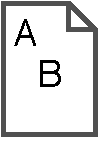
\includegraphics[scale=0.5]{fig/collab/doc-txt-ab.pdf}}
            ](B){
\includegraphics[scale=0.6]{collab/device.pdf}}
            to +(-50:2) node[
                label=below:{Carol},
                label=right:{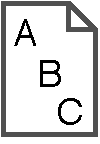
\includegraphics[scale=0.5]{fig/collab/doc-txt-abc.pdf}}
            ](C){
\includegraphics[scale=0.6]{collab/device.pdf}};
        % Links
        \draw[link] (A) to (B);
        \draw[link,-latex] (C) to node[midway]{\includegraphics[scale=0.5]{fig/collab/msg-txt-c.pdf}} (B);
        \draw[link,-latex] (C) to node[midway]{\includegraphics[scale=0.5]{fig/collab/msg-txt-c.pdf}} (A);
    \end{tikzpicture}
    \caption{}\label{fig:op-integration-order-example-1}
\end{subfigure}%
\begin{subfigure}{.5\linewidth}
\centering
    \begin{tikzpicture}
        % devices
        \path (0,0)
            to +(190:2) node[
                label=below:{Alice},
                label=left:{\includegraphics[scale=0.5]{fig/collab/doc-txt-a.pdf}}
            ](A){\includegraphics[scale=0.6]{collab/device.pdf}}
            to +(70:2) node[
                label=above:{Bea},
                label=right:{\includegraphics[scale=0.5]{fig/collab/doc-txt-abc.pdf}}
            ](B){\includegraphics[scale=0.6]{collab/device.pdf}}
            to +(-50:2) node[
                label=below:{Carol},
                label=right:{\includegraphics[scale=0.5]{fig/collab/doc-txt-abc.pdf}}
            ](C){\includegraphics[scale=0.6]{collab/device.pdf}};
        % Links
        \draw[link] (A) to (B);
        \draw[link] (B) to (C);
        \draw[link] (C) to (A);
    \end{tikzpicture}
    \caption{}\label{fig:op-integration-order-example-2}
\end{subfigure}
\caption[Intégration causale d'une opération]{Exemple d'intégration causale d'une opération.
Un ensemble de pairs réplique un texte.
La synchronisation des copies reposent sur une livraison causale des modifications.
\subref{fig:op-integration-order-example-1} Carol insère le caractère $\textsc{'C'}$ à sa copie qui intégré déjà les caractères $\textsc{'A'}$ et $\textsc{'B'}$.
Elle propage sa modification a Alice et Bea.
Pour intégrer le caractère $\textsc{'A'}$ sur une copie, la copie doit déjà contenir les caractères $\textsc{'A'}$ et $\textsc{'B'}$.
Alice n'a pas reçu l'insertion du caractère $\textsc{'B'}$.
Elle ne peut donc pas insérer le caractère $\textsc{'C'}$.
Elle retarde l'intégration de cette modification jusqu'à la réception du caractère $\textsc{'B'}$.
En revanche, la copie de Bea contient déjà les caractères $\textsc{'A'}$ et $\textsc{'B'}$.
\subref{fig:op-integration-order-example-2} Elle intègre donc la modification de Carol.
}\label{fig:op-integration-order-example}
\end{figure}

Généralement, ces protocoles supportent par conception l'édition hors-ligne et en sous-groupes déconnecté·e·s les uns des autres.
Cependant, lorsque les périodes de déconnexion sont longues ou le nombre de modifications hors ligne est important, la synchronisation est coûteuse en communication et en ressources de calcul.
En effet, chaque opération est transmise et intégrée aux copies des pairs.

\paragraph{}Ce qui nous amène à la deuxième question de recherche que nous explorons dans ce manuscrit~: \textbf{Est-il possible de concevoir un protocole de réplication optimiste pour l'édition collaborative de texte en simultané qui intègre immédiatement toute modification et est adapté aux longues périodes de déconnexions~?}

\paragraph{}A notre connaissance, la synchronisation par opérations est le seul schéma de synchronisation utilisé pour l'édition collaborative de texte en simultané.
D'autres schémas de synchronisation ont été proposés pour la conception de protocole de réplication.
La synchronisation par états~\autocite{shapiro_2011_crdt} consiste à transmettre l'état de la copie une fois mise à jour au lieu d'une opération.
Les états sont fusionnés de telle sorte à inclure les mise-à-jours de chacun.
Ce schéma tire son avantage principal du fait qu'un état synthétise l'ensemble des modifications qui ont été précédemment intégrées.
Les états peuvent donc être livrés et intégrés plusieurs fois dans des ordres arbitraires.
Ce qui implique qu'ils peuvent être dupliqués, omis, et réordonnés par le réseau sans compromettre la convergence des copies.
Les pairs peuvent donc intégrer un état dès sa réception.
Il n'y a pas d'intégration retardée d'états.
Par ailleurs, le système est moins sensible aux longues périodes de déconnexions des pairs.
Au lieu de transmettre une longue liste d'opérations, les pairs transmettent simplement l'état de leur copie.

Malgré ces avantages, le schéma de synchronisation par états est resté circonscrit à un petit nombre de protocoles de réplication.
Le schéma implique en effet un coût en communication et en fusion important lorsque les états sont de taille importante.
C'est le cas des copies de contenu textuel.
En effet, il n'est pas raisonnable de transmettre et intégrer l'état d'un document chaque fois qu'un caractère est inséré ou supprimé du document.

Un schéma de synchronisation par différences d'états~\autocite{almeida_2018_delta-crdt-revisited} a récemment été proposé pour tenter de réduire le coût du schéma de synchronisation par états.
Ce schéma autorise toujours la transmission d'états complets.
Cependant, il privilégie l'envoi de différences d'états qui synthétisent une ou plusieurs modifications.
Les différences d'états peuvent être intégrées plusieurs fois dans des ordres arbitraires.
Le schéma de synchronisation par différences d'états offre ainsi de nombreuses possibilités dans la manière de synchroniser deux copies.
Par exemple, lorsque des pairs collaborent en simultané ils peuvent échanger des différences d'états, alors que deux pairs qui se reconnectent après une longue période de déconnexion peuvent échanger directement leur état.

%Contrairement à la synchronisation par opérations, la synchronisation par différences d'états ne retardent pas l'intégration de modification.
%Elle ne propage donc pas de latence dans l'ensemble du système.
%Par ailleurs, sa flexibilité permet de synchroniser deux pairs par l'échange de leur état respectif.
%Lorsque deux pairs se reconnectent après une longue période de déconnexion, ils n'ont pas besoin d'échanger leurs modifications une à une.
%Ils peuvent directement transmettre leur état.
Nous proposons d'adopter ce schéma de synchronisation pour l'édition collaborative de texte.
Pour ce faire, nous concevons un nouveau protocole de réplication optimiste nommé \emph{Dotted LogootSplit}.


\section{Organisation du manuscrit}

Le reste du manuscrit est organisé en 5 chapitres~:

\paragraph{Le \autoref{ch:problematic}} introduit plus en détail les caractéristiques des infrastructures pair-à-pair de collaboration et met l'accent sur les problématiques de recherche liées à la convergence des copies et à sa protection. Le chapitre définit également l'adversaire du système qui contrôle les pairs mal-intentionnés.

\paragraph{Le \autoref{ch:background}} présente les formalismes que nous utilisons dans les chapitres suivants pour décrire nos contributions.
Nous introduisons en particulier la notion de cohérence de données et les types de données répliqués.

%\paragraph{Le \autoref{ch:secured-convergence}} présente notre première contribution qui propose de diviser en deux sous-classes : les \acp{CRDT} étiquetés et les \acp{CRDT} non-étiquetés. Nous montrons que la convergence des \acp{CRDT} non-étiquetés est protéger par conception ou peut être protégé en utilisant un journal infalsifiable. Nous proposons un mécanisme pour protéger les \acp{CRDT} étiquetés synchronisé par opérations.

\paragraph{Le \autoref{ch:pruned-log}} présente deux protocoles qui protègent la convergence des copies des pairs honnêtes.
Le protocole à journaux complets protège la convergence des copies des pairs honnêtes à l'aide de journaux infalsifiables et complets.
Le protocole à journaux tronqués repose sur le protocole à journaux complets.
Il permet la troncature des journaux et l'authentification de l'état d'une copie à l'aide d'un journal tronqué.
Pour développer ce protocole, le chapitre introduit la notion de stabilité et \emph{DynVFJC}, un nouveau modèle de cohérence.
%notre mécanisme pour tronquer un journal infalsifiable. Nous développons \emph{DynVFJC} un modèle de cohérence de donnée basé sur \acl{VFJC} qui permet de stabiliser un journal infalsifiable dans un groupe dont la composition évolué au cours du temps et qui peut inclure des pairs mal-intentionnés. Nous présentons également \acl{VFJCS} qui définit qu'elle partie du journal est stable.
Nous présentons également les travaux de la littérature en relation avec notre protocole.

\paragraph{Le \autoref{ch:dotted-logootsplit}} présente un état de l'art des types séquences de données répliquées.
Nous proposons un modèle unifié pour décrire et mieux appréhender un sous-ensemble de ces types séquence.
À l'aide de ce modèle nous répondons à notre deuxième question de recherche en proposant \emph{Dotted LogootSplit}, le premier type séquence de données répliquées synchronisé par différence d'états.

\paragraph{Le \autoref{ch:conclusion}} clôt ce manuscrit et propose des axes d'exploration pour continuer les travaux de recherche présentés au sein de ce manuscrit.


\section{Publications}

La première contribution développée au sein de ce manuscrit a fait l'objet d'une publication~\autocite{2018_elvinger_prunable-auth-log}.
La seconde contribution présentée n'a pas encore fait l'objet d'une publication.
En revanche, la proposition a été implémentée dans notre prototype d'éditeur collaboratif \emph{MUTE} qui est décrit dans l'une de nos publications~\autocite{2017_nicolas-mute-demo}.
Notre dernière publication~\autocite{2019_yu_genericundo} est en lien avec nos travaux sur les types de données répliquées, mais n'est pas présentée au sein de ce manuscrit.
Dans la suite de cette section nous référençons les articles qui ont été publiés au cours de cette thèse.

\subsection*{Prunable Authenticated Log and Authenticable Snapshot in Distributed Collaborative Systems \autocite{2018_elvinger_prunable-auth-log}}

-- Victorien Elvinger, Gérald Oster, François Charoy

\paragraph{Article de conférence} in proceedings of the 4th {IEEE} International Conference on Collaboration and Internet Computing, ({CIC} 2018)

\paragraph{Abstract:} In distributed collaborative systems, participants maintain a replicated copy of shared documents.
They edit their own copy and then share their modifications without any coordination.
Copies follow successions of divergence and convergence.
Convergence is a liveness property of collaborative systems.
Some malicious participants may find an advantage to make the collaboration fail. 
To that end, they can preclude convergence of the copies.
%
To protect convergence of copies, participants can exploit an authenticated log of modifications.
New participants have to retrieve the entire log in order to contribute. Unfortunately, the cost of joining a collaboration increases with the size of this log.
Causal Stability allows to prune authenticated logs in a static collaborative group without any malicious participants.
%
In this paper, we first tailor Causal Stability to dynamic groups in presence of malicious participants.
We then propose a mechanism to verify the consistency of a pruned log and a mechanism to authenticate a snapshot from a pruned log.

\bigskip
\bigskip

\subsection*{MUTE\@: A Peer-to-Peer Web-based Real-time Collaborative Editor \autocite{2017_nicolas-mute-demo}}

-- Matthieu Nicolas, Victorien Elvinger, Gérald Oster, Claudia-Lavinia Ignat,
François Charoy

\paragraph{Article de démonstration} in proceedings of the 15th European Conference on Computer Supported Cooperative Work ({ECSCW} 2017)

\paragraph{Abstract:} Real-time collaborative editing allows multiple users to edit shared documents at the same time from different places. Existing real-time collaborative editors rely on a central authority that stores user data which is a perceived privacy threat. In this paper, we present \acf{MUTE}, a peer-to-peer web-based real-time collaborative editor without central authority disadvantages. Users share their data with the collaborators they trust without having to store their data on a central place. MUTE features high scalability and supports offline and ad-hoc collaboration.

\clearpage

\subsection*{A Generic Undo Support for State-Based CRDTs \autocite{2019_yu_genericundo}}

-- Weihai Yu, Victorien Elvinger, Claudia-Lavinia Ignat

\paragraph{Article de conférence} in proceedings of the 23rd International Conference on Principles of Distributed Systems, ({OPODIS} 2019)

\paragraph{Abstract:} CRDTs (Conflict-free Replicated Data Types) have properties desirable for large-scale distributed systems with variable network latency or transient partitions.
With CRDT, data are always available for local updates and data states converge when the replicas have incorporated the same updates.
Undo is useful for correcting human mistakes and for restoring system-wide invariant violated due to long delays or network partitions.
There is currently no generally applicable undo support for CRDTs.
There are at least two reasons for this. First, there is currently no abstraction that we can practically use to capture the relations between undo and normal operations with respect to concurrency and causality. 
Second, using inverse operations as the existing partial solutions, the CRDT designer has to hard-code certain rules and design a new CRDT for almost every operation that needs undo support.
In this paper, we present an approach to generic support of undo for CRDTs. The approach consists of two major parts.
We first work out an abstraction that captures the semantics of concurrent undo and redo operations through equivalence classes.
The abstraction is a natural extension of undo and redo in sequential applications and is straightforward to implement in practice.
By using this abstraction, we then device a mechanism to augment existing CRDTs.
The mechanism provides an ``out of the box'' support for undo without the involvement of the CRDT designers.
We also present a practical application of the approach in collaborative editing.



%\section{Infrastructures de collaboration}
%\vicnote{A intégrer dans l'intro}
%
%% flux d'activité = collaborateur + dimension temporel
%
%% mode de collaboration et infras
%Les infrastructures de collaboration permettent à des groupes de collaborateur·ice·s de produire collectivement des contenus.
%Elles restreignent les formes que peuvent prendre ces collaborations.
%Par exemple, l'encyclopédie Wikipedia et le gestionnaire de versions SVN permettent uniquement la modification exclusive d'un contenu ou d'un sous-ensemble d'un contenu.
%Le contenu ne peut être modifié que par un·e seul·e utilisateur·ice à la fois.
%Des gestionnaires de versions distribués comme Git ou Mercurial permettent à plusieurs utilisateur·ice·s de modifier simultanément, mais de manière asynchrone, un même contenu.
%Les utilisateur·ice·s modifient les contenus et se synchronisent à posteriori avec les autres.
%Les éditeurs de textes collaboratifs comme Etherpad ou Goggle Docs permettent à leurs utilisateur·ice·s de modifier simultanément et de manière synchrone un contenu.
%Les utilisateur·ice·s ont l'illusion d'observer les modifications des autres en temps réel.
%\vicnote{Détailler chaque mode de collaboration ?}
%
%En l'absence de restrictions imposées par des infrastructures de collaboration, une activité de collaboration peut prendre différentes formes en fonction des individus et évoluer au cours du temps.
%Reconsidérons l'exemple de l'écriture collaborative d'un logiciel. Des programmeur·euse·s peuvent vouloir modifier de manière isolé une partie du logiciel et se synchroniser à posteriori avec les autres.
%Cette isolation leur permet d'évaluer avec plus de précision l'effet de leurs modifications sur une suite de tests logiciels.
%En revanche, d'autres programmeur·euse·s, éventuellement les mêmes mais à un autre moment, désirent peut être programmer en binômes isolés communément appelé \emph{pair programming}.
%Chaque membre d'un binôme travaille simultanément et de manière synchrone sur un même fichier.
%Cette exemple illustre la diversité des activités de collaboration qui peuvent avoir lieu au sein d'une même équipe qui produit collectivement un contenu.
%Cette composition des modes synchrone et asynchrone est nommée \emph{multi-synchrone} dans la littérature~\autocite{dourish_1995_divergence}.
%
%\vicnote{illustration}
%
%%Les infrastructures traditionnels de collaboration supportent un sous-ensemble des modes d'organisation.
%Les infrastructures traditionnelles de collaboration supportent généralement un sous-ensemble des formes de collaboration.
%Git et Mercurial ne permettent pas une collaboration synchrone.
%Seules les formes asynchrones sont possibles.
%Etherpad et Google Docs ne permettent pas de contribuer à un contenu de manière isolé.
%Les collaboration synchrone requiert une latence faible pour produire l'illusion d'une collaboration en temps réel.
%Elle ne tolère pas les partitions réseaux.
%En revanche les collaboration asynchrone sont tolérantes aux délais, aux pannes, et aux partitions réseaux.
%Elles passent facilement à l'échelle.
%
%% infra P2P
%Les infrastructures pair-à-pair de collaboration ont été conçues pour permettre les collaborations multi-synchrones.
%
%AUTRE EXEMPLES : Nuit debout, télétravail / cours durant la crise du Covid 19.

% BD distribué, DVCS, éditeurs collaboratifs


\chapter{Problématiques}\label{ch:problematic}

\minitoc{}
\bigskip

% Spécifier la convergence
% deux pairs qui observe les mêmes effets d'opérations convergent
% Ici on parle d'op locales, elles peuvent être synchronisées de différentes
% manières.
% L'idée est de se centrer sur la confluence et de se déplacer au niveau de
% la couche réseau.

%La production collective de contenus par plusieurs centaines, voire plusieurs milliers d'utilisateur·ice·s est aujourd'hui une réalité.
%Par exemple, au sein des réseaux sociaux, des milliers d'utilisateur·ice·s réagissent en direct à des évènements et co-organisent des évènements.
%Cependant, la diffusion des activités massives de collaboration reste encore restreinte.
%Cette diffusion se heurte aux limitations conceptuelles des applications et des outils actuels de collaboration.
%Ces limitations sont induites par les infrastructures de collaboration sur lesquelles ils reposent.

Les infrastructures pair-à-pair de collaboration peuvent supporter les activités massives de collaboration.
Elles tolèrent les latences, les pannes, ainsi que les partitions réseaux.
Les collaborateur·ice·s peuvent modifier le contenu partagé de manière isolée.
Des collaborateur·ice·s géographiquement éloigné·e·s ou avec des connexions réseaux lentes et peu fiables peuvent contribuer à une collaboration.
Ces infrastructures sont donc bien adaptées à des collaboration qui impliquent des appareils mobiles.
Pour autant, elles assurent des latences basses lorsque les connexions réseaux le permettent.
Les collaborateur·ice·s ont donc l'illusion d'observer les modifications en temps réel lorsqu'elles et ils modifient simultanément un contenu.
Ces caractéristiques permettent de passer à l'échelle et de respecter le rythme de vie, ainsi que la manière de collaborer de chaque collaborateur·ice.

Pour ce faire, les infrastructures pair-à-pair de collaboration reposent sur la \emph{réplication optimiste}~\autocite{saito_2005_optimisticreplication}.
Chaque collaborateur·ice est associé·e à un pair qui possède une copie du contenu partagé.
Un pair interroge et modifie sa copie indépendemment des autres pairs.
En d'autres termes, les pairs n'ont pas besoin de se coordonner.
La copie est donc \emph{toujours disponible}~\autocite{mahajan_2011_cac} pour être interrogée ou modifiée. % par son/sa collaborateurice
C'est ce qui permet de tolérer les latences et les partitions réseaux.
La modification parallèle des copies conduit inévitablement à leur divergence~: les copies fournissent des réponses distinctes à une ou plusieurs interrogations qui peuvent leur être soumis.
Les pairs échangent à terme leurs modifications.
Les algorithmes de réplication de données sont en charge de la convergence des copies.
Ils doivent s'assurer qu'à terme les copies répondent de manière identique à toutes les interrogations qui peuvent leur être soumit.

La convergence des copies conditionne le succès d'une collaboration.
Si les collaborateur·ice·s ne sont pas capable de partager une vue globalement convergente dans des délais raisonnables, leur collaboration est probablement compromise.
Assurer à terme la convergence des copies est donc important.

Les algorithmes existants de réplication optimiste supposent généralement l'absence de pairs mal-intentionnés.
Plus largement, ils supposent l'absence d'un adversaire actif.
Cette hypothèse n'est pas réaliste au sein d'activités massives de collaboration.
Les pairs mal-intentionnés peuvent mener des attaques pour assurer une divergence permanente des pairs honnêtes.
Ils peuvent ainsi compromettre des collaborations.
Dans ce manuscrit de thèse, nous nous intéressons à cette problématique et nous proposons des mécanismes pour assurer à terme la convergence en présence d'un adversaire actif.

Ce chapitre introduit dans un premier temps la réplication de données. Il développe ensuite la notion de convergence et d'intention des opérations.
Il termine sur le modèle du système auquel nous nous intéressons et il définit l'adversaire du système.

\section{Réplication de données}\label{sec:optimistic-replication}

La réplication de données maintient des copies de contenus partagés sur un ensemble de pairs.
Elle augmente la disponibilité d'un contenu en permettant son interrogation et sa modification en dépit de la défaillance de pairs.
Les répliques sont souvent géographiquement réparties.
Ce qui rapproche les données des utilisateur·ice·s.
Elle réduit donc les latences pour interroger les contenus partagés.

Comparé à un contenu non-répliqué, un contenu répliqué a un nombre étendu de comportements.
Par exemple, des collaborateur·ice·s distinct·e·s peuvent modifier des copies distinctes d'un contenu répliqué.
Ces nouveaux comportements peuvent engendrer des scénarios difficiles à prévoir et traiter.
Idéalement, l'interrogation et la modification d'un contenu répliqué devrait se comporter comme si il existait une seule copie.
Dans ce cas, nous disons que le contenu partagé est \emph{fortement cohérent} et nous parlons de réplication pessimiste de données~\autocite{saito_2005_optimisticreplication}.
La~\autoref{fig:strong-consistency} met en évidence que l'interrogation d'un contenu fortement cohérent prend toujours en compte toutes les modifications précédemment effectuées.

\begin{figure}[htb]
\newcommand*\hsep{2.2}
\newcommand*\vsep{-1.4}
\centering
\begin{subfigure}{\linewidth}
    \centering
    \begin{tikzpicture}
        % Peers
        \node(A) at (0,0) {$p_A$};
        \node(B) at (0,\vsep) {$p_B$};
        \node (C) at (0,2*\vsep) {$p_C$};
        % Events
        \path (A)
            to +(\hsep,0) node[
                label=above:{$\trm{add}(1)$}
            ] (a2) {$\bullet$}
            to +(5*\hsep,0) node (aend) {}
        ;
        \path (B)
            to +(2*\hsep,0) node[
                label=above:{$\trm{rd}\set*{1}$}
            ] (b2){$\bullet$}
            to +(4*\hsep,0) node[
                label=above:{$\trm{rd}\set*{1,2}$}
            ] (b3){$\bullet$}
            to +(5*\hsep,0) node (bend) {}
        ;
        \path (C)
            to +(3*\hsep,0) node[
                label=above:{$\trm{add}(2)$}
            ] (c2) {$\bullet$}
            to +(5*\hsep,0) node (cend) {}
        ;
        % Timeline
        \foreach \src/\dest in {A/a2,B/b2,b2/b3,C/c2,a2/aend,b3/bend,c2/cend}
            \draw[timeline] (\src) to (\dest);
    \end{tikzpicture}
    \caption{}\label{subfig:strong-consistency-trace}
\end{subfigure}
\par\medskip
\begin{subfigure}{\linewidth}
    \centering
    \begin{tikzpicture}
        % Peers
        %\node (space) at (0,1.6) {};
        \node (V) at (0,0) {$p_V$};
        % Events
        \path (V)
            to +(\hsep,0) node[
                label=above:{$\trm{add}(1)$}
            ] (v2) {$\bullet$}
            to +(2*\hsep,0) node[
                label=above:{$\trm{rd}\set*{1}$}
            ] (v3){$\bullet {\scriptstyle}$}
            to +(3*\hsep,0) node[
                label=above:{$\trm{add}(2)$}
            ] (v4) {$\bullet {\scriptstyle}$}
            to +(4*\hsep,0) node[
                label=above:{$\trm{rd}\set*{1,2}$}
            ] (v5){$\bullet {\scriptstyle}$}
            to +(5*\hsep,0) node (vend) {}
        ;
        % Timeline
        \foreach \src/\dest in {V/v2,v2/v3,v3/v4,v4/v5,v5/vend}
            \draw[timeline] (\src) to (\dest);
    \end{tikzpicture}
    \caption{}\label{subfig:strong-consistency-single-copy}
\end{subfigure}
%
\caption[Réplication pessimiste d'un ensemble]{\subref{subfig:strong-consistency-trace} Histoire de l'exécution d'un ensemble répliqué fortement cohérent.
L'ensemble répliqué supporte une opération de modification $\set*{\trm{add}(n) \given n \in \mathbb{N}_0}$ qui ajoute un entier dans l'ensemble, et une opération d'interrogation $\trm{rd}$ qui donne la composition de l'ensemble.
Ainsi l'exécution de l'opération $\trm{add}(1)$ ajoute l'entier $1$ à l'ensemble, et nous notons $\trm{rd} \set*{1}$ une opération de lecture suivit de la valeur retournée par son exécution.
L'ensemble est initialement vide.
Le pair $p_A$ ajoute l'entier $1$.
Ultérieurement le pair $p_C$ ajoute l'entier $2$.
Le pair $p_B$ interroge à deux reprises l'ensemble.
Sa première interrogation se déroule entre les deux ajouts.
La seconde interrogation se déroule après les deux ajouts.
L'ensemble est fortement cohérent, une modification qui survient avant une autre modification ou une interrogation est donc visible à cette dernière.
La première interrogation retourne un singleton composé de l'élément $1$ et la seconde interrogation retourne un ensemble composé des éléments $1$ et $2$.
La cohérence forte maintient l'illusion de l'interrogation et la modification d'une seule copie.
\subref{subfig:strong-consistency-single-copy} L'histoire de l'exécution de cette copie abstraite peut être obtenue en projetant toutes les opérations sur un pair abstrait $p_V$.
}\label{fig:strong-consistency}
\end{figure}

Le maintien de l'illusion de l'interrogation et de la modification d'une seule copie a un coût.
Elle requiert une coordination étroite entre les pairs.
Une coordination qui peut se traduire par des communications systématiques avant chaque modification, voire avant chaque interrogation.
Les latences et les défaillances inhérentes aux réseaux~\cite{rotem_falalcies_2006} rendent cette coordination problématique.
Elle engendre plusieurs problèmes~:

\begin{description}
    \item[Disponibilité.] Le contenu ne peut plus être modifié, voire interrogé, lorsque des pairs sont isolés par des partitions réseaux.
    \item[Latence.] L'interrogation et la modification du contenu partagé est sujet aux latences du réseau et des pairs.
    La lenteur d'un pair ou d'une connexion réseau peut donc affecter l'ensemble du système.
    \item[Passage à l'échelle.] L'ajout de pairs, et donc de copies, peut détériorer la disponibilité et les latences étant donné que le nombre de pairs impliqués dans une coordination augmente.
\end{description}

Le théorème CAP~\cite{brewer_cap_2000,gilbert_cap_2002} montre l'impossibilité de garantir à la fois une cohérence forte et une disponibilité à tout moment en présence de partitions réseaux.
Nous pouvons illustrer cette impossibilité en prenant l'exemple d'une bibliothèque municipale qui possède un système répliqué d'emprunts de livres.
Deux usagers souhaitent faire un emprunt.
Les usagers sont connecté·e·s à des pairs distincts.
Supposons que le réseau est momentanément partitionné de telle manière à ce que les pairs considérés se trouvent dans l'impossibilité de communiquer.
Le système doit faire le choix entre le maintien d'une cohérence forte des emprunts ou la disponibilité d'emprunter.
Le maintien de la cohérence forte empêche tout emprunt tant que les partitions réseaux persistent.
La disponibilité d'emprunter en dépit du partitionnement peut conduire à des conflits.
Par exemple, des usagers peuvent effectuer des emprunts sur la même période d'un livre disponible en un seul exemplaire.

L'illustration proposée pourrait nous amener à penser que la cohérence forte peut être difficilement sacrifiée au bénéfice de la disponibilité.
En effet, le risque d'emprunts conflictuels pourrait produire des situations désagréables pour les usagers et la bibliothèque.
L'illustration proposée souffre du problème de la \emph{double-dépense}~\cite{chohan_doublespending_2017}.
L'emprunt d'un exemplaire d'un livre sur une période donnée correspond à une ressource consommable.
Cette ressource ne peut pas être consommée (dépensée) deux fois.
Ce problème n'est pas toujours rencontré.
Par exemple, un système de pétition en ligne ne souffre pas du problème de la \emph{double-dépense}.
Plusieurs personnes peuvent signer une pétition sans avoir besoin de se coordonner.

Les applications n'ont pas toujours besoin de maintenir une cohérence forte.
En général, le maintien d'une cohérence plus faible est suffisant~\autocite{terry_baseball_2013, hellerstein_calm_2019, decandia_dynamo_2007}.
Prenant cette observation en considération, la \textbf{réplication optimiste}~\autocite{saito_2005_optimisticreplication} sacrifie la cohérence forte pour atteindre une haute disponibilité et des latences basses.
Elle autorise la modification et l'interrogation des copies sans aucune coordination.
Les pairs modifient indépendemment leurs copies et échangeant leurs modifications ultérieurement.
Ce qui conduit à la divergence des copies et à l'intégration des modifications dans des ordres différents.
Deux copies divergentes fournissent des réponses différentes à au moins une interrogation.
La~\autoref{fig:optimistic-replication} illustre un scénario de réplication optimiste.

\begin{figure}[htb]
\newcommand*\hsep{2.2}
\newcommand*\vsep{-1.4}
\centering
\begin{tikzpicture}
    % Peers
    \node(A) at (0,0) {$p_A$};
    \node (B) at (0,\vsep) {$p_B$};
    % Event streams
    \path (A)
        to +(\hsep,0) node[
            label=above:{$\trm{add}(1)$}
        ] (a2) {$\bullet$}
        to +(2*\hsep,0) node[
            label=above:{$\trm{rd}\set*{1}$}
        ] (a3) {$\bullet$}
        to +(3*\hsep,0) node (a4) {$\bullet$}
        to +(4*\hsep,0) node (a5) {$\bullet$}
        to +(5*\hsep,0) node[
            label=above:{$\trm{rd}\set*{1,2}$}
        ] (a6) {$\bullet$}
        to +(6*\hsep,0) node (aend) {}
    ;
    \path (B)
        to +(\hsep,0) node[
            label=below:{$\trm{add}(2)$}
        ] (b2) {$\bullet$}
        to +(2*\hsep,0) node[
            label=below:{$\trm{rd}\set*{2}$}
        ] (b3) {$\bullet$}
        to +(3*\hsep,0) node (b4) {$\bullet$}
        to +(4*\hsep,0) node (b5) {$\bullet$}
        to +(5*\hsep,0) node[
            label=below:{$\trm{rd}\set*{1,2}$}
        ] (b6){$\bullet$}
        to +(6*\hsep,0) node (bend) {}
    ;
    % hb
    \foreach \src/\dest in {A/a2,a2/a3,a3/a4,a4/a5,a5/a6,B/b2,b2/b3,b3/b4,b4/b5,b5/b6,a6/aend,b6/bend}
        \draw[timeline] (\src) to (\dest);
    \draw[hb] (b4) to (a5);
    \draw[hb] (a4) to node[fill=white]{\footnotesize sync} (b5);
\end{tikzpicture}
\caption[Réplication optimiste d'un ensemble]{Exemple de réplication optimiste d'un ensemble.
Les pairs $p_A$ et $p_B$ débutent avec un ensemble vide.
$p_A$ ajoute l'élément $1$ sur sa copie.
$p_B$ ajoute en parallèle l'élément $2$ sur sa copie.
Les copies divergent~: les deux pairs obtiennent des singletons distincts.
Ils synchronisent ultérieurement leurs copies pour échanger et intégrer leurs modifications respectives.
Les modifications ne sont pas intégrés dans le même ordre sur les copies~: ils intégrèrent la modification de l'autre pair après avoir intégré leur propre modification.
Les copies finissent par converger~: les pairs obtiennent le même ensemble.}\label{fig:optimistic-replication}
\end{figure}

Plusieurs modèles de cohérence dits \enquote{faibles} peuvent être respectés par un protocole de réplication optimiste.
L'une des garanties élémentaires de ces modèle concerne la convergence des copies.
En l'absence de modifications, les copies devraient converger.
Toute interrogation sur deux copies convergentes devraient donner les mêmes réponses.
La convergence peut être définit de différentes manières.
La \emph{cohérence à terme}~\autocite{terry_sessionguarentees_1994,saito_2005_optimisticreplication, vogels_eventuallyconsistent_2009} offre la garantie de convergence la plus faible qu'un protocole de réplication optimiste doit respecter.
Elle garantit que deux copies finissent par converger dès lors qu'elles ont intégré le même ensemble de modifications.
Elle garantit également qu'une modification intégrée par un pair finit par l'être par les autres pairs.

\begin{definition}[Cohérence à terme]\label{def:eventual-consistency}
  Une exécution qui respecte la cohérence à terme, respecte les propriétés suivantes~:
  \begin{description}
  \item[\namedlabel{itm:ec1}{EC1} (intégration à terme)] Une modification intégrée sur la copie d'un pair est à terme intégrée par l'ensemble des pairs.
  \item[\namedlabel{itm:ec2}{EC2} (convergence à terme)] Les pairs qui ont intégrés le même ensemble de modifications ont des copies qui convergent à terme.
  \end{description}
\end{definition}

Le fait que la cohérence à terme offre une garantie de convergence si faible suggère que la tâche est difficile.
Cette difficulté réside principalement dans la présence de conflits de modification.
La~\autoref{fig:modif-conflict} présente un scénario où un conflit de modification survient.
La réplication optimiste fait l'hypothèse \textquote{optimiste} que les conflits de modification sont rares et peuvent être résolu ultérieurement.
Les pairs doivent donc gérer les conflits de modification et se mettre d'accord sur un moyen de les résoudre.
Dans la~\autoref{sec:convergence}, nous nous intéressons aux différentes garanties qui peuvent contraindre la convergence et donc la manière de résoudre les conflits de modification.

\begin{figure}[htb]
\newcommand*\hsep{2.2}
\newcommand*\vsep{-1.4}
\centering
\begin{tikzpicture}
    % Peers
    \node(A) at (0,0) {$p_A$};
    \node (B) at (0,\vsep) {$p_B$};
    % Event streams
    \path (A)
        to +(\hsep,0) node[
            label=above:{$\trm{add}(1)$}
        ] (a2) {$\bullet$}
        to +(2*\hsep,0) node[
            label=above:{$\trm{rmv}(1)$}
        ] (a3) {$\bullet$}
        to +(3*\hsep,0) node[
            label=above:{$\trm{rd}\emptyset$}
        ] (a4) {$\bullet$}
        to +(4*\hsep,0) node (a5) {$\bullet$}
        to +(5*\hsep,0) node (a6) {$\bullet$}
        to +(6*\hsep,0) node[
            label=above:{$\trm{rd}\set*{1}$}
        ] (a7) {$\bullet$}
        to +(7*\hsep,0) node (aend) {}
    ;
    \path (B)
        to +(\hsep,0) node[
            label=below:{$\trm{add}(1)$}
        ] (b2) {$\bullet$}
        to +(3*\hsep,0) node[
            label=below:{$\trm{rd}\set*{1}$}
        ] (b3) {$\bullet$}
        to +(4*\hsep,0) node (b4) {$\bullet$}
        to +(5*\hsep,0) node (b5) {$\bullet$}
        to +(6*\hsep,0) node[
            label=below:{$\trm{rd}\emptyset$}
        ] (b6){$\bullet$}
        to +(7*\hsep,0) node (bend) {}
    ;
    % Timeline
    \foreach \src/\dest in {A/a2,a2/a3,a3/a4,a4/a5,a5/a6,a6/a7,B/b2,b2/b3,b3/b4,b4/b5,b5/b6,a6/aend,b6/bend}
        \draw[timeline] (\src) to (\dest);
    \draw[hb] (b4) to (a6);
    \draw[hb] (a5) to node[fill=white]{\footnotesize sync} (b5);
\end{tikzpicture}
\caption[Conflit de modification d'un ensemble répliqué]{Exemple de conflit de modification.
Les pairs $p_A$ et $p_B$ répliquent un ensemble qui supporte une opération d'ajout $\set*{\trm{add}(n) \given n \in \mathbb{N}_0}$, une opération de suppression $\set*{\trm{rmv}(n) \given n \in \mathbb{N}_0}$, et une opération de lecture $\trm{rd}$.
$p_A$ ajoute l'élément $1$ puis le supprime. En parallèle, $p_B$ ajoute également l'élément $1$.
L'ajout et la suppression en parallèle d'un même élément constitue un conflit de modification.
L'élément ne peut pas être à la fois présent et absent de l'ensemble.
L'intégration \textquote{naïve} des modifications dans des ordres distincts conduit à une divergence des copies.}\label{fig:modif-conflict}
\end{figure}


\section{Convergence des copies}\label{sec:convergence}

% coordination -> perf en baisse
% perf en baisse -> moins bonne vivacité ?
% Contraindre plus la convergence pour meilleur vivacité.

% Rappeler que les coordinations sont facteurs de lenteurs ?

Un protocole de réplication optimiste autorise les modifications en concurrence sans coordination.
La divergence des copies est donc inévitable.
Le succès d'une collaboration est conditionné par la capacité des copies à converger.
\textcite{ignat_2015_user-and-delay} ont montré que les activités de collaboration en simultané étaient compromises lorsque le délai entre des modifications de contenu et leurs observations par les autres était trop important.
Dans l'idéal la convergence devrait être atteinte le plus rapidement possible.
Pour réduire au maximum les délais de convergence, toutes coordinations devrait être évitées~\autocite{bailis_coordavoidance_2014}.

\begin{figure}[htb]
\newcommand*\hsep{1.7}
\newcommand*\vsep{-1.4}
\centering
\begin{tikzpicture}
    % Peers
    \node(A) at (0,0) {$p_A$};
    \node (B) at (0,\vsep) {$p_B$};
    % Events
    \path (A)
        to +(\hsep,0) node[
            label=above:{$\trm{add}(1)$}
        ] (a2) {$\bullet$}
        to +(2*\hsep,0) node[
            label=above:{$\trm{rmv}(1)$}
        ] (a3) {$\bullet$}

        to +(3*\hsep,0) node (a4) {$\bullet$}
        to +(4*\hsep,0) node (a5) {$\bullet$}
        to +(5*\hsep,0) node[
            label=above:{$\trm{rd}\set*{1}$}
        ] (a6) {$\bullet$}
        to +(8*\hsep,0) node[
            label=above:{$\trm{rd}\set*{1}$}
        ] (a7) {$\bullet$}
        to +(9*\hsep,0) node (aend) {}
    ;
    \path (B)
        to +(\hsep,0) node[
            label=below:{$\trm{add}(1)$}
        ] (b2) {$\bullet$}

        to +(3*\hsep,0) node (b3) {$\bullet$}
        to +(4*\hsep,0) node (b4) {$\bullet$}
        to +(5*\hsep,0) node[
            label=below:{$\trm{rd}\emptyset$}
        ] (b5){$\bullet$}
        to +(8*\hsep,0) node[
            label=below:{$\trm{rd}\set*{1}$}
        ] (b6){$\bullet$}
        to +(9*\hsep,0) node (bend) {}
    ;
    % Coordinations
    \path (A)
        to ++(6*\hsep,1) coordinate (coord1)
        to node[above,midway,
            label=above:{coordination}
        ]{} +(\hsep,0);
    % Timelines
    \foreach \src/\dest in {A/a2,a2/a3,a3/a4,a4/a5,a5/a6,a6/a7,B/b2,b2/b3,b3/b4,b4/b5,b5/b6,a6/aend,b6/bend}
        \draw[timeline] (\src) to (\dest);
    % Coordination
    \draw[fill=white] (coord1) rectangle +(\hsep,-2+\vsep);
    % Sync
    \draw (b3) edge[hb] (a5);
    \draw (a4) edge[hb] node[fill=white]{\footnotesize sync} (b4);
\end{tikzpicture}
\caption[Réplication optimiste et coordination]{Exemple de coordination après l'intégration de modifications.
Les pairs $p_A$ et $p_B$ intègrent les modifications de chacun.
Les copies ne convergent pas.
Les pairs se coordonnent après l'intégration des modifications afin de converger.}\label{fig:convergence-post-coord}
\end{figure}


Un protocole de réplication optimiste garantit une \emph{convergence à terme} des copies des pairs.
La convergence à terme assure seulement que les pairs qui ont intégrés un même ensemble de modification convergeront dans un futur plus ou moins proche.
Elle ne donne aucune borne sur le temps nécessaire et le nombre de communications nécessaires  pour converger.
La \autoref{fig:convergence-post-coord} illustre un scénario dans lequel deux pairs intègrent leurs modifications respectives et se coordonnent ensuite afin de converger.

Cette propriété de convergence est faible car il s'agit d'une propriété de vivacité.
Une propriété de vivacité peut être violée en plusieurs points de l'exécution d'un protocole~\autocite{alpern_liveness_1985}.
Elle décrit \enquote{quelque chose de positif} qui devrait survenir.
La formulation d'une propriété de vivacité inclut généralement l'expression \enquote{à terme}.

Afin de faire converger plus rapidement les copies et exclure l'utilisation de coordinations, nous devons contraindre la convergence avec des propriétés de sûreté.
Une propriété de sûreté décrit \enquote{quelque chose de mauvais} qui ne devrait jamais survenir.
Une propriété de sûreté doit être respectée en tout point de l'exécution d'un protocole.
\textcite{shapiro_2011_crdt} proposent la \emph{convergence forte} comme propriété de sûreté de la convergence.

\begin{definition}[Convergence forte]\label{def:strong-convergence}
Les pairs qui ont intégré le même ensemble de modifications ont des copies convergentes.
\end{definition}

La \emph{convergence forte} ne nécessite pas de coordinations après l'intégration des modifications.
Cependant, elle n'exclut pas l'utilisation de coordination avant l'intégration des modifications.
Les pairs peuvent décider d'un moyen de résoudre les éventuels conflits de modification.
Par exemple, un protocole peut utiliser un pair privilégié qui ordonne les modifications selon un ordre global~\autocite{terry_bayou_1995}.
\textcite{mahajan_2011_cac} proposent la \emph{convergence unidirectionelle} pour éviter toutes coordinations.
L'idée centrale de la \emph{convergence unidirectionelle} est que deux pairs $p_A$ et $p_B$ devraient être capable de faire converger leur copie en deux étapes de communication unidirectionelle~: $p_A$ envoie des modifications à $p_B$, puis $p_B$ envoie des modifications à $p_A$.

%\begin{definition}[Convergence partielle]\label{def:partial-convergence}
%$p_A$ \emph{converge partiellement} avec $p_B$ si et seulement si il suffit que
%\begin{enumerate}[label=(\roman*)]
%\item $p_A$ et $p_B$ arrêtent de modifier leur copie et de communiquer avec les autres pairs
%\item $p_B$ transmette à $p_A$ les modifications qu'il a intégré et $p_A$ intègre ces dernières
%\end{enumerate}
%pour que les copies de $p_A$ et $p_B$ convergent.
%\end{definition}
%
%\begin{definition}[Convergence unidirectionelle]\label{def:one-way-convergence}
%Pour tout pair $p_A$ qui arrête de modifier sa copie et de communiquer avec tout pair, il suffit que $p_A$ transmette à $p_B$ les modifications qu'il a intégré et que $p_B$ intègre ces dernières pour que $p_A$ \emph{converge partiellement} avec $p_B$.
%\end{definition}
%
%\vicnote{Y-a t-il un intérêt à renforcer cette propriété ? Non... => supprimer ce qui arrive après ?}
%
%Nous pouvons renforcer cette propriété en exigeant que deux pairs $p_A$ et $p_B$ soient capable de converger en initiant deux communications unidirectionnelles en concurrence~: $p_A$ envoie des modifications à $p_B$, et $p_B$ envoie en parallèle des modifications à $p_A$.
%
%\begin{definition}[Convergence unidirectionelle forte]\label{def:strong-one-way-convergence}
%Si $p_A$ et $p_B$ arrêtent de modifier leur copie et arrêtent de communiquer avec les autres pairs, alors il suffit que
%\begin{enumerate}[label=(\roman*)]
%\item $p_A$ transmette à $p_B$ les modifications qu'il a intégré
%\item $p_B$ transmette (éventuellement en parallèle) à $p_A$ les modifications qu'il a intégré
%\item $p_A$ et $p_B$ intègrent (éventuellement en parallèle) les modifications qu'ils ont reçu de chacun
%\end{enumerate}
%pour que leurs copies convergent.
%\end{definition}

La non-nécessité de coordination pour obtenir des copies convergentes, suggère une résolution déterministe des conflits de modification.
Dans le cas de la bibliothèque, on peut supposer que dans la majorité des cas des emprunts simultanés concernent des livres ou des exemplaires différents sur des périodes distinctes.
Toutefois, des conflits d'emprunts peuvent survenir.
Le nombre d'exemplaires d'un nouveau livre peut être insuffisant par rapport au nombre de lecteur·ice·s intéressé·e·s.
Plusieurs stratégies peuvent être mises en place pour résoudre ces conflits.
On peut considérer que l'emprunteur·ice final·e correspond à la personne qui a fait l'emprunt en premier.

%Au fil des modifications et de leurs échanges, les pairs suivent des cycles de divergence et de convergence.


% \section{Intention des opérations}

% Il peut exister plusieurs manière de réconcilier les copies d'un contenu partagé.
% Dans la \autoref{fig:optimistic-replication}, les pairs intègrent les ajouts de chaque pair afin de converger vers un état équivalent.
% Cependant, rien n'empêche de réconcilier les copies en rejetant les ajouts effectuées en parallèle.
% Les pairs $p_A$ et $p_B$ pourraient ainsi converger vers un ensemble vide.

% Cette approche de réconciliation pourrait surprendre les collaborateur·ice·s.
% En effet, si deux éléments sont ajoutés en parallèle dans l'ensemble, on pourrait s'attendre à ce qu'ils appartiennent dans l'ensemble après la réconciliation des copies.
% \textcite{sun_1998_cci} parlent d'intention des opérations.
% Intuitivement, l'intention d'une opération capture l'effet observable de l'opération.
% Cette effet devrait être observable quelque soit le pair qui exécute l'opération.

% L'intégration d'opération concurrentes ou plus largement la réconciliation de copies devrait préserver autant que possible l'intention des opérations qui sont exécutées.
% L'intention d'une opération peut être exprimée comme une postcondition.
% Cette postcondition doit être prudemment spécifiée afin d'assurer son respect quelque soit l'ordre d'exécution des opérations qui sont indépendantes de l'opération considérée.
% Les opérations indépendantes correspondent aux opérations concurrentes et éventuellement à d'autres opérations.

% Reprenons l'exemple de l'ensemble répliqué pour illustrer la spécification de l'intention des opérations.
% Le type abstrait de donnée Ensemble spécifie l'ajout d'un élément dans un ensemble comme l'ensemble auquel a été ajouté l'élément.
% Dans un premier temps nous pouvons définir l'intention de l'ajout d'un élément comme sa spécification.
% Dans la \autoref{fig:optimistic-replication} l'opération $\trm{add}(1)$ a comme intention l'obtention du singleton $\set*{1}$.
% L'opération $\trm{add}(2)$ a comme intention l'obtention du singleton $\set*{2}$.
% La réconciliation des copies des deux pairs conduit nécessairement à la violation de l'intention de l'une des opérations.
% Nous pouvons définir plus prudemment l'intention des opérations de telle manière à ce qu'elle offre une garantie pertinente tout en évitant leur violation.
% Dans notre cas, nous pouvons définir l'intention d'un ajout comme l'obtention d'un ensemble qui contient à la fois l'élément ajouté et les éléments précédemment ajoutés.
% La présence d'éléments ajoutés en concurrence n'est donc pas exclut.
% Dans la \autoref{fig:optimistic-replication} l'opération $\trm{add}(1)$ a comme intention l'obtention d'un ensemble qui contient l'élément $1$.
% L'opération $\trm{add}(2)$ a comme intention l'obtention d'un ensemble qui contient l'élément $2$.

% % Intention -> No rollbacks
% La préservation de l'intention des opérations peut plus largement retranscrire le principe d'intégrer les opérations de chaque pair sans les ignorer.
% Ce qui empêche la mise en place de retour en arrière.


\section{Modèle du système}

\vicnote{Figure à mettre à jour}

\begin{figure}[htb]
\centering
\includegraphics{fig/impl.pdf}
\caption{Une infrastructure de collaboration composée de 3 pairs qui répliquent le contenu partagé. Les 3 pairs sont connectés par un réseau asynchrone.}\label{fig:collab-system}
\end{figure}

Dans les infrastructure pair-à-pair de collaboration, chaque collaborateur·ice est associé·e à un pair qui lui est exclusif.
\textcite{guerraoui_2016_tradeoffs-replication} parlent de \emph{sticky availability}.
L'une des principales implications est que des pairs peuvent joindre et quitter le système de réplication au gré des connexions et des déconnexions des collaborateur·ice·s.
De nouveaux pairs peuvent joindre lorsque de nouveaux et nouvelles collaborateur·ice·s joignent le groupe
Des pairs existants peuvent se déconnecter indéfiniment lorsque les collaborateur·ice·s associé·e·s quittent le groupe.

Pour interroger et modifier le contenu partagé, un·e collaborateur·ice soumet des opérations au pair qui lui est associé.
Ces opérations dépendent du type du contenu répliqué.
Dans la~\autoref{fig:optimistic-replication}, l'ensemble répliqué peut être modifié par une opération d'ajout $\set*{\trm{add}(n) \given n \in \mathbb{N}_0}$ et peut être intérrogé par une opération de lecture $\trm{rd}$ qui donne la composition de l'ensemble.
Les opérations sont d'abord intégrées sur la copie que le pair détient.
Les pairs synchronisent leur copie en arrière plan.
Une synchronisation peut s'effectuer après chaque nouvelle modification ou peut être espacée dans le temps.

Nous supposons qu'un·e collaborateur·ice ne peut être dissocié·e du pair qui lui est attaché.
La copie est donc \emph{toujours disponible}~\autocite{mahajan_2011_cac} pour être interrogée et modifiée.


\section{Adversaire du système}

Un protocole de réplication optimiste doit respecté un ensemble de propriétés de cohérence.
Pour assurer ces propriétés, un protocole doit résister aux défaillances et aux comportements mal-intentionnés qu'il rencontre au cours de ses exécutions.
Par exemple, il doit se prémunir contre les défaillances inhérentes aux réseaux.

Les protocoles de réplication optimiste supposent généralement l'absence de comportements mal-intentionnés.
Cette hypothèse n'est pas réaliste au sein d'activités massives de collaboration.
Plus un groupe de collaborateur·ice·s est large plus il est probable que le groupe inclut un ou plusieurs utilisateur·ice·s mal-intentionné·e·s.

Les défaillances d'un système peuvent être accidentelles ou résultantes de comportements mal-intentionnés.
Sans perte de généralité, nous considérons que toute défaillance est le résultat de comportements mal-intentionnés.
Ces comportements sont exprimés par l'adversaire du système.
L'adversaire du système est mû par un objectif et contrôle des ressources, tels que le réseau et des pairs, pour atteindre son objectif.

L'objectif de notre adversaire est de compromettre la convergence des copies des collaborateur·ice·s honnêtes~\footnote{Dans la littérature le terme \textquote{correct} est également utilisé.}.
Et ce dans le but de faire échouer leur collaboration.
Pour simplifier les références ultérieures, nous proposons de classifier les capacités de l'adversaire à travers trois profils~: réseau asynchrone non-fiable, réseau corrompu, pairs perturbées, pairs mal-intentionnés.

\paragraph{Réseau asynchrone non-fiable.} L'adversaire contrôle le réseau et peut exposer l'ensemble des comportements observées sur un réseau asynchrone non-fiable~\autocite{lynch_1996_asyncnet}.
En particulier, les messages échangées entre les pairs peuvent être réordonnés, dupliqués, retardés, et omis.
L'adversaire peut séparer les pairs en partitions.
Toutefois il ne peut pas empêcher les pairs honnêtes de s'échanger à terme un nombre non-borné de messages.
Ce qui implique qu'il ne peut pas maintenir indéfiniment une partition réseau ou omettre tous les messages émit par un pair.
Cette limitation est nécessaire pour que des propriétés de vivacité, tel que l'\emph{intégration à terme}, soient réalisables.

\paragraph{Réseau asynchrone corrompu.} L'adversaire a les limitations et les capacités décrites dans le profil \emph{réseau asynchrone non-fiable}.
En outre, il peut contrefaire des messages.
Il peut par exemple changer l'émetteur d'un message ou le contenu d'un message.

\paragraph{Pairs restaurés.} L'adversaire peut perturber un pair honnête.
Il peut le soumettre à des lenteurs arbitraires.
Il ne peut toutefois pas empêcher un pair de progresser dans l'exécution du protocole.
L'adversaire peut également produire des pannes qui rend momentanément le pair indisponible.
Nous supposons que les pairs honnêtes disposent d'une mémoire durable et fiable de telle sorte à ce qu'ils retrouvent l'état dans lequel ils se trouvaient juste avant leur dernière panne.
Pour les mêmes raisons que celles évoqués dans le profil \emph{réseau asynchrone non-fiable}, l'adversaire ne peut pas provoquer des pannes dans l'objectif d'arrêter l'exécution définitive du protocole ou d'empêcher indéfiniment les pairs honnêtes de s'échanger un nombre non-borné de messages.

\paragraph{Pairs mal-intentionnés.} L'adversaire contrôle un ensemble de pairs mal-intentionnés~\footnote{Dans la littérature, le terme \textquote{défectueux} est également utilisé.} qui peuvent librement travailler de concert. Il peut librement connecter de nouvelles pairs mal-intentionnés et déconnecter, éventuellement indéfiniment, des pairs mal-intentionnés. Les pairs mal-intentionnés peuvent se comporter de manière arbitraire.

\paragraph{}L'adversaire peut utiliser l'ensemble de ses capacités et de ses ressources pour exprimer des comportements complexes.
Toutefois, nous supposons les limitations suivantes~:

\begin{itemize}
  \item L'adversaire a des ressources limitées en puissance de calcul et en temps.
  Ces ressources ne sont pas suffisantes pour compromette les primitives de cryptographies, telles que les signatures digitales et les fonctions de hachage résistants aux collisions.
  \item Il ne peut pas empêcher un pair honnête d'authentifier la clef publique d'un autre pair honnête.
  L'adversaire ne peut pas obtenir la clef privé d'un pair honnête et il ne peut donc pas usurper son identité cryptographique.
\end{itemize}

Les protocoles de réplication optimiste s'intéressent généralement à un adversaire qui a les profils \emph{réseau asynchrone non-fiable} et \emph{pairs restaurés}.
En ajoutant les deux autres profils \emph{réseau corrompu} et \emph{pairs mal-intentionnés} nous obtenons un adversaire qui est Byzantin~\autocite{lamport_1982_byzantinegeneralsproblem}.

Certain·e·s auteur·ice·s font la distinction entre les pairs mal-intentionnés et les pairs honnêtes-mais-défaillants.
Un pair honnête-mais-défaillant expose des comportements qui peuvent être prêtés à un pair mal-intentionné.
Un pair honnête n'a pas la capacité de décider si un comportement nuisible d'un pair est le résultat d'une défaillance ou de motivations mal-intentionnées.
Nous considérons donc les pairs honnêtes-mais-défaillants comme des pairs mal-intentionnés.


\section{Synthèse et objectifs}

Un protocole de réplication optimiste autorise la modification et l'interrogation des copies d'un contenu répliqué sans aucune coordination.
Les copies sont donc toujours disponible pour être modifiées et interrogées.
La modification concurrente des copies conduit inévitablement à leur divergence.
La convergence des copies est une propriété essentielle des infrastructures de collaboration.
Elle conditionne le succès d'une collaboration.
Afin d'assurer des latences faibles et un passage à l'échelle du protocole, nous nous intéressons à des propriétés de convergence qui ne nécessitent pas de coordination.

Le passage à l'échelle et les latences faibles des protocole de réplication optimiste auxquels nous nous intéressons permet le support de collaboration massive.
Ce type de collaboration à une probabilité plus importante de rencontrer des comportements mal-intentionnés.
Nous avons choisi de nous intéresser à des protocoles qui résistent à un adversaire Byzantin.
Ce dernier contrôle le réseau et un ensemble de pairs mal-intentionnés.
Il peut également perturber le fonctionnement des pairs honnêtes.

Dans ce manuscrit nous cherchons à assurer la convergence des copies des pairs honnêtes sans la nécessité de coordination.


\chapter{Fondations}\label{ch:background}

\minitoc{}
\bigskip

Dans ce chapitre, nous introduisons les formalismes et les concepts que nous utilisons pour définir les contributions du \autoref{ch:pruned-log} et du \autoref{ch:dotted-logootsplit}.

Les infrastructures pair-à-pair de collaboration permettent à un nombre important d'individus de collaborer.
Pour ce faire elles reposent sur des protocoles de réplication optimiste.
Les protocoles de réplication optimiste garantissent des \emph{propriétés de cohérence} des copies aux pairs et par extension aux collaborateur·ice·s.
La convergence des copies est l'une de ces propriétés de cohérence.
La \autoref{sec:consistency-spec} introduit le formalisme que nous utilisons pour décrire les propriétés de cohérence.
Notre formalisme étend le formalisme de~\textcite{burckhardt_eventualconsistency_2014} pour prendre en compte la présence d'un adversaire actif.
Les protocoles de réplication garantissent souvent des ensembles communs de propriétés de cohérence.
Pour faciliter l'appréciation de leurs similitudes, les propriétés de cohérence sont réunies sous des ensembles bien définies nommés \emph{modèle de cohérence}.
La \autoref{sec:consistency-spec} présente également un moyen de comparer les modèles de cohérence.
La \autoref{sec:causal-models} présente le modèle de cohérence causale ainsi que les modèles de cohérence sur-lesquelles nous nous reposons pour établir la contribution du \autoref{ch:pruned-log}.

La convergence des copies est une propriété essentielle des protocoles de réplication optimiste.
Dans le \autoref{ch:problematic}, nous avons motivé notre intérêt pour des protocoles qui permettent la convergence des copies sans coordination.
De tels protocoles n'imposent pas aux pairs de dialoguer pour s'entendre sur la manière de résoudre les conflits de modification qui surviennent au cours de la collaboration.
Ils n'ont d'autres choix que d'adopter des résolutions prédéterminées de conflit.
Les protocoles de réplication optimiste décident en général la manière de résoudre un conflit.
Pour faciliter la comparaison des protocoles et leur implémentation, les stratégies de résolution de conflits sont encapsulées au sein de type de données répliquées nommés \acfp{CRDT}.
Les concepteur·ice·s d'applications peuvent ainsi utiliser des type de données prêt à l'emploi.
La \autoref{sec:crdt} présente ces types de données et illustre plusieurs sémantiques de résolution de conflits.

\section{Spécification de modèles de cohérence}\label{sec:consistency-spec}

Un protocole détermine comment un pair peut interagir de manière conforme avec le système.
En délimitant le périmètre d'action des pairs, le protocole garantit des propriétés de cohérence des copies.
\textcite{burckhardt_eventualconsistency_2014} a introduit un formalisme pour décrire des propriétés de cohérence et modéliser l'exécution d'un protocole.
Le formalisme qu'il introduit n'est pas adapté aux environnements soumis à la présence de pairs mal-intentionnés.
Dans la \autoref{subsec:consistency-spec-honest} nous présentons son formalisme avec quelques simplifications.
Nous l'étendons dans la \autoref{subsec:consistency-spec-malicious} pour permettre la description d'exécutions soumises à la présence de comportements mal-intentionnés.

Les propriétés de cohérence sont groupées en ensembles logiques dénommés \emph{modèles de cohérence}.
Les modèles de cohérence sont organisés en hiérarchie de celui qui offre les garanties de cohérence les plus fortes à ceux qui offrent les garantie les plus faibles.

Dans le \autoref{ch:problematic} nous avons distingué les propriétés de sûreté des propriétés de vivacité.
Dans la \autoref{subsec:consistency-spec-liveness-safety} nous montrons comment reconnaître et spécifier ces deux genres de propriétés au sein du formalisme introduit.

%Nous motivons d'abord l'intérêt d'exprimer des garanties de cohérence et nous détaillons le formalisme introduit par \textcite{burckhardt_eventualconsistency_2014}.
%Nous étendons ensuite ce formalisme à des environnement qui tolèrent la présence de pairs mal-intentionnés.
%Nous terminons par définir ce qu'est un modèle de cohérence, comment comparer des modèles de cohérence, et une classification possible des garanties de cohérence entre garanties de vivacité et garanties de sûreté. 

\subsection{Spécification en l'absence de pairs mal-intentionnés}\label{subsec:consistency-spec-honest}

Les collaborateur·ice·s s'attendent à ce que les infrastructures de collaboration leur offrent un certain nombre de garanties de cohérence des copies du contenu partagé.
La \autoref{fig:causal-expectation} illustre un scénario dans lequel Bea s'attend à ce que Alice lise les messages textuels dans l'ordre dans lequel elle les a écrit.
Certains protocoles de réplication optimiste peuvent respecter les attentes de Bea et d'autres peuvent ne pas les respecter.
Les attentes des collaborateur·ice·s sont exprimées sous la forme de propriétés de cohérence.

% EXEMPLE : SMS texting, matrix protocol

\begin{figure}[htb]
\centering
\begin{tikzpicture}
    \newcommand*\hsep{2.2}
    \newcommand*\vsep{-1.4}
    % Peers
    \path node (A) {$p_A$}
        to +(0,\vsep) node (B) {$p_B$}
    ;
    % Timeline ends
    \path (7*\hsep,0) coordinate (aend)
        to +(0,\vsep) coordinate (bend)
    ;
    % Events
    \path (A)
        to +(\hsep,0) node[
            label=above:{$\trm{rd}\emptyset$}
        ] (a1) {$a_1$}
        to +(4*\hsep,0) node[
            label=above:{$\trm{rd}\set*{t_2}$}
        ] (a2) {$a_2$}
        to +(6*\hsep,0) node[
            label=above:{$\trm{rd}\set*{t_1,t_2}$}
        ] (a3) {$a_3$}
    ;
    \path (B)
        to +(\hsep,0) node[
            label=below:{$\trm{rd}\emptyset$}
        ] (b1) {$b_1$}
        to +(2*\hsep,0) node[
            label=below:{$\trm{post}(t_1)$}
        ] (b2) {$b_2$}
        to +(3*\hsep,0) node[
            label=below:{$\trm{post}(t_2)$}
        ] (b3) {$b_3$}
    ;
    % Timelines
    \foreach \src/\dest in {A/a1,a1/a2,a2/a3,B/b1,b1/b2,b2/b3,a3/aend,b3/bend}
        \draw (\src) edge[timeline] (\dest);
\end{tikzpicture}
\caption[Attentes des collaborateur·ice·s]{Alice (pair $p_A$) et Bea (pair $p_B$) discutent sur un fil de discussion répliqué.
Le fil de discussion répliqué supporte une opération d'ajout d'un message textuel $\set*{\trm{post}(\trm{txt}) \given \trm{txt} \in \trm{String} }$, et une opération de lecture $\trm{rd}$.
L'exécution d'une opération de lecture retourne l'ensemble des messages qui ont été ajoutés.
Ainsi l'exécution de l'opération $\trm{post}(t_1)$ permet d'ajouter le message textuel $t_1$ sur le fil de discussion.
Nous notons $\trm{rd} s$ l'exécution d'une opération de lecture suivie de l'ensemble $s$ de messages textuels qu'elle retourne.
Bea ajoute un premier message $t_1$ suivi d'un second message $t_2$.
Elle s'attend à ce que Alice prenne connaissance du premier message avant de prendre connaissance du second message.
Cependant, le protocole ne lui garantit pas cette propriété.
Alice lit le second message avant de lire le premier.}\label{fig:causal-expectation}
\end{figure}

Les propriétés de cohérence sont de différentes natures.
Certaines contraignent l'ordre dans lequel les modifications sont intégrées par les pairs.
D'autres spécifient la valeur retournée par les interrogations des pairs.
Elles expriment toutes des garanties qui sont offertes aux collaborateur·ice·s.
De ce fait, elles s'expriment sur les interactions des collaborateur·ice·s avec le protocole et sur les réponses que le protocole fournit aux collaborateur·ice·s.
Les collaborateur·ice·s interagissent avec le système en exécutant des opérations.
L'ensemble des opérations exécutées forme une \emph{histoire}.
L'histoire de la \autoref{fig:causal-expectation} est constituée des trois opérations de Alice (pair $p_A$) et des trois opérations de Bea (pair $p_B$).

Les collaborateur·ice·s exécutent des opérations de modifications pour altérer l'état du contenu partagé et exécutent des opérations d'interrogation pour observer les effets de leurs modifications.
Nous supposons que tout type de contenu partagé est interrogé avec une unique opération $\trm{rd}$.
Il s'agit de l'\emph{opération de lecture}.

Nous supposons que l'exécution d'une opération se termine et qu'elle se déroule sur un intervalle de temps non-nul.
Les dates de début et de fin d'exécution des opérations sont issues d'une unique horloge à temps continu.
Cette horloge n'a pas d'existence propre au cours d'une exécution réelle.
Nous avons toutefois besoin d'un temps continu et universel pour exprimer certaines propriétés de cohérence.

Lorsque nous raisonnons sur l'exécution d'opérations, nous nous intéressons souvent à l'ordre dans lequel les opérations sont exécutées.
Les dates de début et de fin d'exécution d'une opération fournissent plus d'information que nécessaire.
Pour faciliter le raisonnement sur l'ordre d'exécution des opérations d'une histoire, nous introduisons la relation suivante~:

\paragraph{Retourne-avant~\autocite{burckhardt_eventualconsistency_2014}.} Une relation d'ordre partiel qui rend compte des opérations dont l'exécution ne coïncide pas dans le temps.
Une opération $x$ retourne-avant une opération $y$, et nous écrivons $x \rb y$, si et seulement si l'exécution de $x$ se termine avant que l'exécution de $y$ débute.
Si $x$ ne retourne pas avant $y$ et si $y$ ne retourne pas avant $x$, alors leur exécution coïncide.
La \autoref{fig:rb-example} montre un exemple de deux opérations dont l'exécution coïncide dans le temps.

\begin{figure}[ht]
\centering
\begin{subfigure}{.5\linewidth}
    \centering
    \begin{tikzpicture}
        \newcommand*\hsep{1.6}
        \newcommand*\vsep{-1.4}
        % Peers
        \path node (A) {$p_A$}
            to +(0,\vsep) node (B) {$p_B$}
        ;
        % Timeline ends
        \path (4*\hsep+0.5,0) coordinate (aend)
            to +(0,\vsep) coordinate (bend)
        ;
        % Events
        \path (A)
            to +(1,0) node[
                label=above:{$\trm{rd}\emptyset$},
                timedevt,minimum width=1.5cm
            ] (a1) {}
        ;
        \path (B)
            to +(2,0) node[
                label=below:{$\trm{rd}\emptyset$},
                timedevt,minimum width=1cm
            ] (b1) {}
            to +(8*0.5,0) node[
                label=below:{$\trm{post}(t_1)$},
                timedevt,minimum width=2cm
            ] (b2) {}
        ;
        % Timelines
        \foreach \src/\dest in {A/a1,B/b1,b1/b2,a1/aend,b2/bend}
            \draw[timeline] (\src) to (\dest);
    \end{tikzpicture}
    \caption{}\label{fig:rb-example-1}
\end{subfigure}%
\begin{subfigure}{.5\linewidth}
    \centering
    \begin{tikzpicture}
        \newcommand*\hsep{1.6}
        \newcommand*\vsep{-1.4}
        % Peers
        \path node (A) {$p_A$}
            to +(0,\vsep) node (B) {$p_B$}
        ;
        % Timeline ends
        \path (4*\hsep+0.5,0) coordinate (aend)
            to +(0,\vsep) coordinate (bend)
        ;
        % Events
        \path (A)
            to +(\hsep,0) node[
                label=above:{$\trm{rd}\emptyset$}
            ] (a1) {$\bullet$}
        ;
        \path (B)
            to +(\hsep,0) node[
                label=below:{$\trm{rd}\emptyset$}
            ] (b1) {$\bullet$}
            to +(3*\hsep,0) node[
                label=below:{$\trm{post}(t_1)$}
            ] (b2) {$\bullet$}
        ;
        % Timelines
        \foreach \src/\dest in {A/a1,B/b1,a1/aend,b2/bend}
            \draw[timeline] (\src) to (\dest);
        % returns-before
        \draw[-latex] (a1) to node[above,sloped] {\footnotesize rb} (b2);
        \draw[-latex] (b1) to node[above,sloped] {\footnotesize rb} (b2);
    \end{tikzpicture}
    \caption{}\label{fig:rb-example-2}
\end{subfigure}
\caption[Relation retourne-avant d'une histoire]{\subref{fig:rb-example-1} L'intervalle de temps sur lequel l'opération d'interrogation de Alice ($p_A$) s'exécute a une intersection non-nulle avec l'intervalle de temps sur lequel l'opération d'interrogation de Bea ($p_B$) s'exécute.
Ces deux opérations coïncident donc dans le temps.
En revanche, l'intervalle de temps sur lequel l'opération de modification de Bea s'exécute a une intersection nulle avec les deux opérations d'interrogation.
Elle ne coïncide donc pas dans le temps avec ces deux opérations d'interrogation.
Dans ce manuscrit, les propriétés de cohérence que nous exprimons ne nécessitent pas la connaissance de l'intervalle de temps sur lequel une opération s'exécute.
\subref{fig:rb-example-2} Nous contractons donc les intervalles en des points.
Deux points alignés verticalement correspondent à des opérations dont l'exécution coïncide dans le temps.
Si l'exécution de deux opérations ne coïncide pas, alors une opération \emph{retourne-avant} l'autre.
Ici, cette information est explicitement marquée par l'utilisation de la relation \emph{retourne-avant} $\rb$.}\label{fig:rb-example}
\end{figure}

\paragraph{}La \autoref{def:history} définit formellement une histoire.
Elle définit en particulier les caractéristiques associées aux opérations.
La \autoref{tab:op-attributes} donne les caractéristiques des opérations de l'histoire de la \autoref{fig:causal-expectation}.

\begin{definition}[histoire~\autocite{burckhardt_eventualconsistency_2014}]\label{def:history}
Une \emph{histoire} d'un contenu partagé de type $T$ est un n-uplet $H \defeq \tuple*{E, \trm{peer}, \trm{call}, \trm{rval}, \trm{rb}}$ tel que $E$ est un ensemble dénombrable d'opérations.
Pour toute opération $x$~:
\begin{itemize}
\item $\trm{peer}(x) \in \trm{Peers}$ est l'auteur de l'opération $x$.
\item $\trm{call}(x) \in \trm{Op}_T$ est l'appel effectué par l'auteur de $x$.
Ces appels dépendent de $T$.
\item $\trm{rval}(x) \in \trm{Val}_T$ est la valeur de retour de l'appel de $x$ si il s'agit d'une interrogation.
Ces valeurs de retour dépendent de $T$.
\end{itemize}
\begin{itemize}[leftmargin=*]
\item[] $\trm{rb} \subseteq E \times E$ est la relation \emph{retourne-avant}.
Il s'agit d'un ordre partiel localement fini\footnote{Pour tout couple d'opérations, l'ensemble des opérations comprises entre ces 2 opérations est fini.} qui peut être interprété sur une ligne de temps\footnote{\textcite{greenough_1976_semiorder} parle d'ordre d'intervalle.}~:
\begin{equation*}
    u \rb v \land y \rb z \implies u \rb z \lor y \rb v
\end{equation*}
\end{itemize}
\end{definition}

\begin{table}[ht]
    \centering
    \begin{tabular}{cccc}
        opération & $\trm{peer}$ & $\trm{call}$ & $\trm{rval}$ \\
        \toprule
        $a_1$ & $p_A$ & $\trm{rd}$ & $\emptyset$ \\
        $a_2$ & $p_A$ & $\trm{rd}$ & $\set*{t_2}$ \\
        $a_3$ & $p_A$ & $\trm{rd}$ & $\set*{t_1, t_2}$ \\
        $b_1$ & $p_B$ & $\trm{rd}$ & $\emptyset$ \\
        $b_2$ & $p_B$ & $\trm{post}(t_1)$ & \\
        $b_3$ & $p_B$ & $\trm{post}(t_2)$ & \\
    \end{tabular}
    \caption{Caractéristiques des opérations exécutées dans l'histoire de la \autoref{fig:causal-expectation}.
    Un fil de discussion supporte une opération de lecture et une opération de modification $\trm{Op}_T = \set*{\trm{rd}} \cup \set*{\trm{post}(\trm{msg}) \given \trm{msg} \in \trm{String}}$.
    Les valeurs de retour correspondent à des ensembles de messages $\trm{Val}_T = \powerfset{\trm{String}}$. $\powerfset{\trm{String}}$ est l'ensemble des sous-ensembles finis des chaînes de caractères.}\label{tab:op-attributes}
\end{table}

Un protocole garantit une propriété de cohérence si et seulement si toutes les histoires qu'il peut produire vérifient cette propriété.
Une histoire vérifie une propriété de cohérence si et seulement si ses caractéristiques (valeur de retour des opérations, ordre d'exécution, \ldots) peuvent être expliquées par l'ajout de la relation suivante~:

\paragraph{Visibilité~\autocite{burckhardt_eventualconsistency_2014}.} Une relation qui rend compte de l'intégration des effets des opérations de modification par les pairs.
Si une opération de modification $x$ est visible à une opération d'interrogation $y$, alors $x$ a (éventuellement) un effet sur la valeur de retour de $y$.
Nous disons aussi que l'effet de $x$ a été intégré à la copie avant l'exécution de l'opération $y$ sur cette même copie.
%Si une opération $x$ est visible à une opération $y$ alors la première a été intégrée par le pair avant l'exécution de $y$.
Dans ce cas, nous écrivons $x \vis y$.
La relation de visibilité n'est pas forcément transitive.
Par exemple, dans la \autoref{fig:vis-example}, $b_2$ est visible à $b_3$ et $b_3$ est visible à $a_2$, mais $b_2$ n'est pas visible à $a_2$.
Par souci de concision, nous écrivons $x \viseq y$ si $x$ est visible ou est égal à $y$.

% Nous pourrions nous contenter des histoires pour exprimer des propriétés de cohérences.
% En procédant de la sortes nos propriétés mélangent des contraintes d'ordre et des contraintes de type.
% Afin de séparer les contraintes nous exprimant nos propriétés de cohérence à l'aide d'exécution abstraites.

\paragraph{} Une histoire augmentée de la relation de \emph{visibilité} consiste en une \emph{exécution abstraite}~\autocite{burckhardt_eventualconsistency_2014}.
La \autoref{def:abstract-exec} définit formellement une exécution abstraite.
La \autoref{fig:vis-example} est une exécution abstraite de l'histoire de la \autoref{fig:causal-expectation}.

\begin{definition}[exécution abstraite~\autocite{burckhardt_eventualconsistency_2014}]\label{def:abstract-exec}
Une \emph{exécution abstraite} d'un contenu partagé de type $T$ est un n-uplet $A \defeq \tuple*{H, \trm{vis}}$ tel que~:
\begin{itemize}
  \item $H$ est une histoire d'un contenu partagé de type $T$.

  \item $\trm{vis} \subseteq H \times H$ est la relation de \emph{visibilité}. Elle est sans cycle et localement finie.
\end{itemize}
\end{definition}

\begin{figure}[bth]
\centering
\begin{tikzpicture}
    \newcommand*\hsep{2.2}
    \newcommand*\vsep{-1.4}
    % Peers
    \path node (A) {$p_A$}
        to +(0,\vsep) node (B) {$p_B$}
    ;
    % Timeline ends
    \path (7*\hsep,0) coordinate (aend)
        to +(0,\vsep) coordinate (bend)
    ;
    % Events
    \path (A)
        to +(\hsep,0) node[
            label=above:{$\trm{rd}\emptyset$}
        ] (a1) {$a_1$}
        to +(4*\hsep,0) node[
            label=above:{$\trm{rd}\set*{t_2}$}
        ] (a2) {$a_2$}
        to +(6*\hsep,0) node[
            label=above:{$\trm{rd}\set*{t_1,t_2}$}
        ] (a3) {$a_3$}
    ;
    \path (B)
        to +(\hsep,0) node[
            label=below:{$\trm{rd}\emptyset$}
        ] (b1) {$b_1$}
        to +(2*\hsep,0) node[
            label=below:{$\trm{post}(t_1)$}
        ] (b2) {$b_2$}
        to +(3*\hsep,0) node[
            label=below:{$\trm{post}(t_2)$}
        ] (b3) {$b_3$}
    ;
    % Timelines
    \foreach \src/\dest in {A/a1,a1/a2,a2/a3,B/b1,b1/b2,a3/aend,b3/bend}
        \draw[timeline] (\src) to (\dest);
    % Visibility
    \draw[vis] (b2) to node[above] {\footnotesize vis} (b3);
    \draw[vis] (b3) to node[above,sloped] {\footnotesize vis} (a2);
    \draw[vis,bend left=40] (b2) to node[above,sloped] {\footnotesize vis} (a3);
    \draw[vis] (b3) to node[above,sloped] {\footnotesize vis} (a3.south west);
\end{tikzpicture}
\caption[Exécution abstraite]{Une \emph{exécution abstraite} de l'histoire de la \autoref{fig:causal-expectation}.
La relation \emph{retourne-avant} est inférée par le positionnement horizontal des opérations.
}\label{fig:vis-example}
\end{figure}

Une histoire vérifie une propriété de cohérence si et seulement si il existe au moins une exécution abstraite qui la respecte.
Il suffit donc de générer toutes les exécutions abstraites possibles pour une histoire donnée et vérifier que au moins l'une d'entre elles respecte la propriété de cohérences considérée.
La \autoref{fig:hist-absexec} met en évidence les relations entre histoires, exécutions abstraites, et propriétés de cohérence.

\begin{figure}[tbh]
\centering
\newcommand*\psep{1}
\newcommand*\bsq{\scriptscriptstyle\blacksquare}
\begin{tikzpicture}
    \begin{scope}[inner sep=0]
        % histories
        \path (0,0) node{$\bullet$}
            to +(30:\psep) node (h3) {$\bullet_1$}
            to +(90:\psep) node {$\bullet$}
            to +(150:\psep) node {$\bullet$}
            to +(210:\psep) node {$\bullet$}
            to +(270:\psep) node {$\bullet$}
            to +(330:\psep) node (h6) {$\bullet_2$}
            ;
        % abstract exec
        \path (7,0) node (A4) {$\bsq_2$}
            to +(0:\psep) node (A5) {$\bsq$}
            to +(120:\psep) node (A1) {$\bsq_1$}
            to +(180:\psep) node (A3) {$\bsq$}
            to +(240:\psep) node (A7) {$\bsq_3$}
            ;
        \path (7 + 2*\psep,0) node (A6) {$\bsq$}
            to +(120:\psep) node (A2) {$\bsq$}
            to +(240:\psep) node (A8) {$\bsq_4$}
            ;
    \end{scope}
    \begin{scope}[rounded corners]
        % boxes
        \node[
            draw, fit=(h3) (h6),
            pin={-100:{du protocole $P$}}
        ] {};
        \node[
            draw, fit=(A1) (A3) (A4) (A7),
            pin={-100:{respectant $p_1$}}
        ] {};
        \node[
            draw, fit=(A2) (A5) (A6) (A8),
            pin={-80:{respectant $p_2$}}
        ] {};
        \node[
            draw, fit=(A4) (A5),
            pin={[pin distance=50]30:{respectant $p_3$}}
        ] {};
    \end{scope}
    \begin{scope}[bend left=10]
        % relations
        \draw (h3) to (A1);
        \draw (h3) to (A4);
        \draw (h6) to (A7);
        \draw (h6) to (A8);
    \end{scope}
    % sep
    \draw (3,2.5) node[
            label={below left:{ensemble des \emph{histoires}}},
            label={below right:{ensemble des \emph{exécutions abstraites}}},
        ] {}
        to +(0,-5)
        ;
\end{tikzpicture}
\caption[Relations entre protocoles, histoires, exécutions abstraites, et propriétés de cohérence]{Illustration des relations entre protocoles, histoires, exécutions abstraites, et propriétés de cohérence.
L'exécution du protocole $P$ peut produire les histoires $\bullet_1$ et $\bullet_2$.
$\bsq_1$ et $\bsq_2$ correspondaient aux exécutions abstraites que nous obtenons à partir de $\bullet_1$.
$\bsq_3$ et $\bsq_4$ correspondaient aux exécutions abstraites que nous obtenons à partir de $\bullet_2$.
L'histoire $\bullet_1$ vérifié les propriétés de cohérence $p_1$ et $p_3$ puisque l'exécution abstraite $\bsq_2$ les respectent.
De même, l'histoire $\bullet_2$ vérifié la propriété $p_1$ ou $p_2$ puisque l'exécution abstraite $\bsq_3$ respecte $p_1$ et l'exécution abstraite $\bsq_4$ respecte $p_2$.
Le protocole $P$ garantit ainsi la propriété $p_1$ puisque chacune de ses histoires est associée à au moins une exécution abstraite qui la respecte.}\label{fig:hist-absexec}
\end{figure}

La relation de visibilité rend compte de l'intégration des effets des opérations de modification par les pairs.
En tant que tel, seules les relations de visibilité dirigées d'une opération de modification vers une opération d'interrogation semblent faire sens.
Dans la \autoref{fig:vis-example} on remarque ainsi que l'effet de l'opération $b_3$ est pris en compte par l'opération de lecture $a_2$, et les effets des opérations $b_2$ et $b_3$ sont pris en compte par l'opération de lecture $a_3$.
Notre définition de la relation de visibilité nous permet de mettre en relation tout type d'opérations.
Dans la \autoref{fig:vis-example} il existe ainsi une relation de visibilité entre les opérations de modification $b_2$ et $b_3$.
Cette flexibilité nous permet de simplifier l'expression des propriétés de cohérence.

Les relations précédemment définies sont suffisantes pour exprimer toutes les propriétés de cohérence auxquelles nous nous intéressons dans ce manuscrit\footnote{\textcite{burckhardt_eventualconsistency_2014} ajoute également une relation d'arriération $\trm{ar}$ à ses exécutions abstraites. Elle s'avère utile dans la définition de certains type de données répliquées. Nous l'avons délibérément omise par souci de simplification.}.
Ces expressions peuvent parfois être peu lisibles.
Par exemple, pour spécifier le type de retour d'une opération de lecture, il est nécessaire de prendre en compte l'ensemble des opérations de modification qui sont visibles à cette opération de lecture.
Dans la \autoref{fig:vis-example}, si un ajout de message textuel est visible à une opération de lecture, alors cette dernière inclut ce message dans sa valeur de retour.
Pour faciliter l'expression de telles propriétés, nous introduisons dans la \autoref{def:op-context} le \emph{contexte} d'une opération.
Le contexte d'une opération regroupe les opérations de modifications qui lui sont visibles.
La \autoref{tab:op-ctx-obs} donne le contexte des opérations de l'exécution abstraite de la \autoref{fig:vis-example}.

\begin{definition}[Contexte]\label{def:op-context}
Le \emph{contexte} d'une opération $x$ dans une \emph{exécution abstraite} $A$, dénoté par $\trm{ctx}_A(x)$, correspond à l'ensemble des opérations de modification\footnote{\textcite{burckhardt_eventualconsistency_2014,viotti_consistency_2016} incluent également les opérations d'interrogation dans le contexte d'une opération. Nous les excluons pour simplifier l'expression de certaines propriétés de cohérence.} qui lui sont visibles.
\begin{equation*}
    \trm{ctx}_A(x) \defeq \set*{y \in A \given y \vis x \land \trm{op}(y) \neq \trm{rd}}
\end{equation*}
\end{definition}

\begin{table}[htb]
    \centering
    \begin{tabular}{ccc}
        Opération & $\trm{ctx}$ & $\trm{obs}$ \\
        \toprule
        $a_1$ & $\emptyset$ & $\set*{p_A}$ \\
        $a_2$ & $\set*{b_3}$ & $\set*{p_A}$ \\
        $a_3$ & $\set*{b_2, b_3}$ & $\set*{p_A}$ \\
        $b_1$ & $\emptyset$ & $\set*{p_B}$ \\
        $b_2$ & $\emptyset$ & $\set*{p_A, p_B}$ \\
        $b_3$ & $\emptyset$ & $\set*{p_A, p_B}$ \\
    \end{tabular}
    \caption{Contexte et observateurs des opérations de l'exécution abstraite de la \autoref{fig:vis-example}.}\label{tab:op-ctx-obs}
\end{table}

La spécification du type de données répliquées de la \autoref{fig:causal-expectation} (fil de discussion) peut ainsi être exprimé par l'\autoref{eq:chat-spec}~:

\begin{equation}\label{eq:chat-spec}
    x \in A \land \trm{call}(x) = \trm{rd} \implies \trm{rval}(x) = \set*{t \given \exists y \in \trm{ctx}_A(x) \qsep \trm{call}(y) = \trm{post}(t)}
\end{equation}

L'exécution abstraite de la \autoref{fig:vis-example} respecte cette propriété de cohérence.
L'histoire de la \autoref{fig:causal-expectation} respecte donc cette propriété de cohérence.


%Un protocole définit les opérations que les pairs peuvent exécuter.
%Lors d'une exécution d'un protocole, les pairs exécutent ainsi un ensemble d'opérations.
%Ces opérations forment l'histoire de l'exécution.
%Le protocole garantit une propriété de cohérence des copies si l'ensemble des histoires qui peuvent être obtenues lors de son exécution vérifient cette propriété.
%Les exécutions abstraites facilitent la définition et la vérification des propriétés de cohérence.
%Une exécution abstraite consiste en une histoire augmentée de la relation de visibilité.
%La relation de visibilité rend compte de l'intégration des opérations modifications par les pairs.
%À une histoire correspond plusieurs exécutions abstraites.
%Il suffit qu'une exécution abstraite respecte une propriété de cohérence pour que l'histoire qui lui correspond la vérifie également.
%Les propriétés de cohérence sont de simples prédicats définit sur les exécutions abstraites.

Le formalisme présenté nous permet de définir des propriétés de cohérence comme de simples prédicats sur des exécutions abstraites.
Des propriétés de cohérence sont garanties par un protocole si chaque histoire du protocole peut être augmentée en une exécution abstraite qui les respecte toutes.
~\textcite{burckhardt_eventualconsistency_2014} a défini les histoires et les exécutions abstraites avec l'hypothèse que les pairs  suivent le protocole.
Nous proposons de généraliser le formalisme pour qu'il puisse être utilisé en présence de pairs qui peuvent déroger au protocole.
Nous qualifions ces pairs de mal-intentionnés.


\subsection{Spécification en présence de pairs mal-intentionnés}\label{subsec:consistency-spec-malicious}

%Un protocole offre des garanties de cohérence uniquement aux pairs qui le suivent, c'est à dire aux pairs honnêtes.
%Les pairs mal-intentionnés peuvent librement déroger à un protocole.
%Ils peuvent par exemple exécuter des opérations qui ne sont pas reconnues par le protocole.
%
%Il n'est donc pas nécessaire de relever l'ensemble des interactions initiées par les pairs mal-intentionnés. Nous nous intéressons uniquement aux opérations qui sont prises en compte par les pairs honnêtes.
%Il s'agit des opérations observées par au moins un pair honnête.

Dans cette section nous proposons une extension du formalisme de \textcite{burckhardt_eventualconsistency_2014}.
Cette extension permet de décrire des exécutions dans lesquels des pairs peuvent déroger au protocole.
Nous qualifions ces pairs de \emph{mal-intentionnés}.
Inversement, les pairs qui suivent le protocole sont qualifiés d'\emph{honnêtes}.
Nous notons $\trm{Honest}$ et $\trm{Malicious}$ l'ensemble des pairs honnêtes et mal-intentionnés.
L'union de ces deux ensemble correspond à l'ensemble des pairs $\trm{Peers}$.
Ces ensembles sont connus étant donné que nous décrivons des exécutions d'un point de vue global.

Sans perte de généralité, nous supposons que les pairs honnêtes exécutent les opérations de manière séquentielle.
Les opérations exécutées sur un même pair sont donc linéairement ordonnées selon la relation \emph{retourne-avant}.
Elles forment une énumération.
Les opérations d'un pair honnête peuvent donc être numérotées dans l'ordre dans lequel elles sont exécutées.
Dans la \autoref{fig:vis-example} on observe ainsi deux énumérations $a_1 \rb a_2 \rb a_3$ et $b_1 \rb b_2 \rb b_3$.
Une histoire qui remplie cette condition est une \emph{histoire bien-formée}.
La \autoref{def:wf-history-malicious} définit formellement une histoire bien-formée.

\begin{definition}[histoire bien-formée]\label{def:wf-history-malicious}
En présence de pairs mal-intentionnés, une histoire $H$ est \emph{bien-formée} si et seulement si pour tout pair honnête $h$, la projection de la relation \emph{retourne-avant} sur $h$ forme une énumération.
%$\tuple*{H|_p, \trm{rb}}$ est une énumération pour tout pair honnête $p$.
%$H|_p$ correspond à l'ensemble des opérations exécutées sur le pair honnête $p$.
\begin{equation*}
x, y \in H \land \trm{peer}(x) \in \trm{Honest} \land \trm{peer}(x) = \trm{peer}(y) \implies x \rb y \lor y \rb x
\end{equation*}
\end{definition}

Les pairs mal-intentionnés peuvent librement déroger à un protocole.
Ils peuvent par exemple~:
\begin{itemize}
    \item Exécuter des opérations qui ne se terminent pas
    \item Exécuter des opérations qui ne sont pas reconnues par le protocole
    \item Produire des interactions qui ne peuvent pas être caractérisées par des opérations
\end{itemize}
Un protocole offre des garanties de cohérence uniquement aux pairs qui le suivent, c'est-à-dire aux pairs honnêtes.
Ces garanties se vérifient donc sur ce que les pairs honnêtes prennent en compte.
Seuls les interactions acceptées par les pairs honnêtes sont incluses dans une histoire.

Les pairs honnêtes acceptent uniquement les interactions reconnues par le protocole.
En d'autres termes ils rejettent toutes les interactions qui ne correspondent pas à des opérations définies par le protocole.
Au sein d'une exécution abstraite, une opération est acceptée par les pairs honnêtes si et seulement si elle est exécutée par un pair honnête ou si elle est visible à au moins une opération exécutée par un pair honnête.
Une opération acceptée est ainsi observée par au moins un pair honnête.
La \autoref{def:op-obs} définit ce qu'est un observateur d'une opération.
La \autoref{tab:op-ctx-obs} donne les observateurs de chaque opération de l'histoire de la \autoref{fig:causal-expectation}.

\begin{definition}[Observateurs]\label{def:op-obs}
Soit une opération $x$ d'une exécution abstraite $A$.
Un pair $p$ est un observateur de $x$ si et seulement si \begin{inlinelist}\item $p$ a exécuté $x$ ou \item $p$ a exécuté une opération de $A$ tel que $x$ est visible à cette dernière\end{inlinelist}.
$\trm{obs}_A(x)$ désigne l'ensemble des observateurs de $x$.
\begin{equation*}
  \trm{obs}_A(x) \defeq \set*{ \trm{peer}(y) \given y \in A \land x \viseq y}
\end{equation*}
\end{definition}

Une \emph{exécution abstraite bien-formée} inclut uniquement les opérations qui sont observées par les pairs honnêtes.
Ces opérations correspondent \begin{inlinelist}
    \item aux opérations exécutées par les pairs honnêtes et
    \item aux opérations exécutées par des pairs mal-intentionnés qui sont visibles à au moins une opération d'un pair honnête
\end{inlinelist}.
La \autoref{def:wf-abstract-exec-malicious} définit formellement une exécution abstraite bien-formée.
La \autoref{fig:wf-example} donne un exemple d'exécution abstraite mal-formée et d'une exécution abstraite bien-formée.
%Les pairs mal-intentionnés peuvent exécuter des opérations qui ne se terminent pas.
%Parce qu'elles ne se terminent pas, elles ne peuvent pas être observées par d'autres pairs, en particulier par les pairs honnêtes.
%Les pairs mal-intentionnés peuvent exécuter des opérations arbitraires.
%Les pairs honnêtes observent uniquement les opérations possible pour le contenu qu'ils partagent.

\begin{definition}[exécution abstraite bien-formée]\label{def:wf-abstract-exec-malicious}
    En présence de pairs mal-intentionnés, une \emph{exécution abstraite} $A \defeq \tuple*{H, \trm{vis}}$ est \emph{bien-formée} si et seulement si~:
    \begin{description}
      \item[\namedlabel{itm:bf1}{BF1}] $H$ est une \emph{histoire bien-formée}.
    
      \item[\namedlabel{itm:bf2}{BF2}] Les opérations dans $E$ des pairs mal-intentionnés sont chacune visible à au moins une opération d'un pair honnête.
      \begin{equation*}
        x \in A \land \trm{peer}(x) \notin \trm{Honest} \implies \trm{obs}_A(x) \cap \trm{Honest} \neq \emptyset
        %\exists y \in A \qsep x \vis y \land \trm{peer}(y) \in \trm{Honest}
      \end{equation*}
    \end{description}
\end{definition}

\begin{figure}[tbh]
\centering
\begin{subfigure}{.5\linewidth}
    \centering
    \begin{tikzpicture}
        \newcommand*\hsep{1.5}
        \newcommand*\vsep{-1.2}
        % Peers
        \path node (A) {$p_A$}
            to +(0,\vsep) node (M) {$p_M$}
            to +(0,2*\vsep) node (B) {$p_B$}
        ;
        % Timeline ends
        \path (4*\hsep,0) coordinate (aend)
            to +(0,\vsep) coordinate (mend)
            to +(0,2*\vsep) coordinate (bend)
        ;
        % Events
        \path (A)
            to +(\hsep,0) node[] (a1) {$a_1$}
        ;
        \path (M)
            to +(2*\hsep,0) node[] (m1) {$m_1$}
        ;
        \path (B)
            to +(\hsep,0) node[] (b1) {$a_1$}
        ;
        % Timelines
        \foreach \src/\dest in {A/a1,B/b1,M/m1,a1/aend,b1/bend,m1/mend}
            \draw[timeline] (\src) to (\dest);
        % visibility
        \draw[vis] (a1) to node[above,sloped] {\footnotesize vis} (m1);
        \draw[vis] (b1) to node[above,sloped] {\footnotesize vis} (m1);
    \end{tikzpicture}
    \caption{}\label{fig:wf-example-1}
\end{subfigure}%
\begin{subfigure}{.5\linewidth}
    \centering
    \begin{tikzpicture}
        \newcommand*\hsep{1.5}
        \newcommand*\vsep{-1.2}
        % Peers
        \path node (A) {$p_A$}
            to +(0,\vsep) node (M) {$p_M$}
            to +(0,2*\vsep) node (B) {$p_B$}
        ;
        % Timeline ends
        \path (4*\hsep,0) coordinate (aend)
            to +(0,\vsep) coordinate (mend)
            to +(0,2*\vsep) coordinate (bend)
        ;
        % Events
        \path (A)
            to +(\hsep,0) node[] (a1) {$a_1$}
            to +(3*1.5,0) node[] (a2) {$a_1$}
        ;
        \path (M)
            to +(2*\hsep,0) node[] (m1) {$m_1$}
        ;
        \path (B)
            to +(\hsep,0) node[] (b1) {$a_1$}
        ;
        % Timelines
        \foreach \src/\dest in {A/a1,a1/a2,B/b1,M/m1,a2/aend,b1/bend,m1/mend}
            \draw (\src) edge[timeline] (\dest);
        % visibility
        \draw[vis] (a1) to node[above,sloped] {\footnotesize vis} (m1);
        \draw[vis] (b1) to node[above,sloped] {\footnotesize vis} (m1);
        \draw[vis] (m1) to node[above,sloped] {\footnotesize vis} (a2);
    \end{tikzpicture}
    \caption{}\label{fig:wf-example-2}
\end{subfigure}
\caption{Soit un groupe de pairs composé d'un pair mal-intentionné $p_M$ et de deux pairs honnêtes $p_A$ et $p_B$.
L'exécution abstraite \subref{fig:wf-example-1} n'est pas bien-formée.
L'opération $m_1$ est uniquement observée par un pair mal-intentionné $p_M$.
L'exécution abstraite \subref{fig:wf-example-2} est bien-formée.
L'opération $m_1$ est observée par le pair honnête $p_A$.}\label{fig:wf-example}
\end{figure}

\begin{remark}
Dans la suite de ce manuscrit nous considérons uniquement, sauf explicitement indiqué, des histoires et des exécutions abstraites bien-formées.
Par souci de concision, nous omettons de préciser qu'une histoire ou une exécution abstraite est bien-formée.
\end{remark}

Les pairs mal-intentionnés peuvent faire coïncider dans le temps l'exécution de plusieurs opérations.
La \autoref{fig:no-enum-example} illustre ce scénario.
Pour pouvoir numéroter les opérations des pairs mal-intentionnés, nous utiliserons des exemples dans lesquels les pairs mal-intentionnés exécutent leurs opérations de manière séquentielle.
%Nous suivrons cet ordre pour numéroter les opérations des pairs mal-intentionnés sauf si il gène la compréhension d'un exemple.

\begin{figure}[htb]
\centering
\begin{subfigure}{.5\linewidth}
    \centering
    \begin{tikzpicture}
        % Peers
        \node (M) at (0,0) {$p_M$};
        % Events
        \path (M)
            to +(1,0) coordinate (mfork)
            to +(2,0.3) coordinate (mfork1)
            to +(2,-0.3) coordinate (mfork2)
        ;
        \path (mfork1)
            to +(1,0) node[
                timedevt,minimum width=1.5cm
            ] (m1) {}
            to +(9*0.5,0) coordinate (mfork1end)
        ;
        \path (mfork2)
            to +(1.5,0) node[
                timedevt,minimum width=1.5cm
            ] (m2) {}
            to +(9*0.5,0) coordinate (mfork2end)
        ;
        % Timelines
        \foreach \src/\dest in {M/mfork,mfork/mfork1,mfork1/m1,mfork/mfork2,mfork2/m2,m1/mfork1end,m2/mfork2end}
            \draw[timeline] (\src) to (\dest);
    \end{tikzpicture}
    \caption{}\label{fig:no-enum-example-1}
\end{subfigure}%
\begin{subfigure}{.5\linewidth}
    \centering
    \begin{tikzpicture}
        % Peers
        \node (M) at (0,0) {$p_M$};
        % Events
        \path (M)
            to +(1,0) coordinate (mfork)
            to +(2,0.3) coordinate (mfork1)
            to +(2,-0.3) coordinate (mfork2)
        ;
        \path (mfork1)
            to +(1.5,0) node[] (m1) {$\bullet$}
            to +(9*0.5,0) coordinate (mfork1end)
        ;
        \path (mfork2)
            to +(1.5,0) node[] (m2) {$\bullet$}
            to +(9*0.5,0) coordinate (mfork2end)
        ;
        % Timelines
        \foreach \src/\dest in {M/mfork,mfork/mfork1,mfork1/m1,mfork/mfork2,mfork2/m2,m1/mfork1end,m2/mfork2end}
            \draw[timeline] (\src) to (\dest);
    \end{tikzpicture}
    \caption{}\label{fig:no-enum-example-2}
\end{subfigure}
\caption{Mallory est une collaboratrice mal-intentionnée.
Elle est attachée au pair $p_M$.
\subref{fig:no-enum-example-1} Les exécutions des deux opérations de Mallory coïncident dans le temps.
\subref{fig:no-enum-example-2} Exemple d'une exécution abstraite correspondante.}\label{fig:no-enum-example}
\end{figure}

%L'adaptation présentée nous permet de décrire des exécutions de protocoles qui incluent des pairs mal-intentionnés.

La généralisation du formalisme de~\textcite{burckhardt_eventualconsistency_2014} que nous proposons nous permet de décrire des exécutions qui incluent des pairs mal-intentionnés.
Ces descriptions nous permettent de rendre compte des propriétés de cohérence qu'un protocole garantit en présence de pairs mal-intentionnés.



\subsection{Vivacité et sûreté}\label{subsec:consistency-spec-liveness-safety}

La littérature divise les propriétés de cohérence entre propriétés de sûreté et propriétés de vivacité.
Une propriété de sûreté décrit \enquote{quelque chose de mauvais} qui ne devrait jamais survenir~\autocite{lamport_1977_correctness}.
Elle doit être respectée en tout point de l'exécution d'un protocole.
Il s'agit d'un invariant.
Une propriété de vivacité décrit \enquote{quelque chose de positif} qui devrait survenir~\autocite{lamport_1977_correctness}.
Elle peut être violée en plusieurs points de l'exécution d'un protocole.
Une propriété de cohérence peut être la conjonction d'une propriété de sûreté et d'une propriété de vivacité~\autocite{alpern_liveness_1985}.

Dans ce chapitre nous avons déjà rencontré plusieurs propriétés de sûreté telles que l'\autoref{eq:chat-spec} qui spécifie le fil de discussion.
En revanche, nous n'avons pas rencontré de propriétés de vivacité.
Dans le \autoref{ch:problematic}, l'intégration à terme des modifications est une propriété de vivacité.
Elle pourrait être traduite par la propriété de cohérence suivante~: une opération de modification est à terme visible à toute opération future d'interrogation.
Nous pouvons prendre avantage de la flexibilité de la relation de visibilité pour simplifier l'expression à~: une opération est à terme visible à toute opération future.
En d'autres termes, pour toute opération il n'existe pas une infinité d'opérations auxquelles elle n'est pas viisble.
Nous pouvons ainsi définir la propriété d'intégration à terme que nous renommons volontiers en propriété de visibilité à terme~:

\begin{equation}
    %\forall x \in A\ \exists A_1 \sqsupseteq A\ \forall A_2 \sqsupset A_1, y \in A_2 \sminus A_1 \qsep x \vis y
    \forall x \in A \qsep \set*{y \in A \given x \not\vis y} \textit{est fini}
\end{equation}

Pour terminer la définition du modèle de cohérence à terme forte, nous définissons également la propriété de sûreté de convergence forte~:

\begin{equation}
    \forall x, y \in A \qsep \trm{call}(x) = \trm{call}(y) = \trm{rd} \land \trm{ctx}_A(x) = \trm{ctx}_A(y) \implies \trm{rval}(x) = \trm{rval}(y)
\end{equation}

Dans ce manuscrit, la propriété de convergence forte est impliquée par les spécifications de types de données répliquées.
C'est le cas dans l'\autoref{eq:chat-spec} qui spécifie le fil de discussion.
Deux opérations de lecture qui ont le même contexte ont nécessairement la même valeur de retour.

Les propriétés de vivacité nous invitent à penser les futures possibles d'une exécution.
En effet, nous devons vérifier que la propriété est vérifiable dans un futur potentiel.

% Un protocole garantit une propriété de cohérence si et seulement si chacune des exécutions abstraites qu'il peut engendrer la respecte.
% Nous ne pouvons pas savoir à quel moment une propriété de vivacité sera respectée.
% Par exemple, la propriété d'intégration à terme des effets des opérations ne donne aucune borne sur le temps nécessaire pour la satisfaire.
% Nous ne pouvons donc pas savoir si un protocole vérifie une telle propriété en raisonnant uniquement sur des exécutions finies.
% Nous devons raisonner également sur des exécutions infinies.
% La \autoref{def:abstract-exec} permet la description d'exécutions abstraites infinies.
% En effet, l'ensemble des opérations exécutées est dénombrable, mais peut être non-fini.
% Une exécution abstraite respecte donc une propriété de vivacité si et seulement si il existe une extension qui la respecte.

% Dans le cas d'une propriété de sûreté, il est nécessaire de vérifier que la propriété est respectée en chaque point des exécutions possibles du protocole.
%Chaque point d'une exécution peut être restreint en une exécution abstraite (bien-formée).
%Ces exécutions abstraites correspondent à des préfixes finis de l'exécution abstraite finale.


\begin{definition}[Extension d'une histoire]\label{def:hist-ext}
Une histoire $H'$ est une extension d'une histoire $H$, et nous écrivons $H' \sqsupset H$, si et seulement si~:
\begin{itemize}
  \item Les opérations de $H$ correspondent à un sous-ensemble fini des opérations de $H'$. $H$ est donc une histoire finie.

  \begin{equation*}
    H \subset H' \land H \textit{est finie}
  \end{equation*}

  \item Si l'opération $y$ est incluse dans $H$, alors toutes les opérations de $H'$ qui retournent-avant $y$ sont également incluses dans $H$.
  \begin{equation*}
    y \in H \land x \rb_{H'} y \implies x \in H
  \end{equation*}
  
  \item Les relations \emph{retourne-avant} sont conservées.
  \begin{equation*}
    x, y \in H \land x \rb_{H'} y \iff x \rb_{H} y
  \end{equation*}
  
  \item Les caractéristiques des opérations (pair, appel, valeur de retour) sont conservées.
\end{itemize}
\end{definition}


\begin{definition}[Extension d'une exécution abstraite]\label{def:wf-abstract-exec-prefix}
Une exécution abstraite $A' \defeq \tuple*{H',\trm{vis}'}$ est une extension d'une exécution abstraite (bien-formée ou mal-formée) $A \defeq \tuple*{H,\trm{vis}}$, et nous écrivons $A' \sqsupset A$, si et seulement si~:
\begin{itemize}
  \item L'histoire $H'$ de $A'$ est une extension de l'histoire $H$ de $A$~:

  \begin{equation*}
    H' \sqsupset H
  \end{equation*}

  \item Les relations de visibilité sont conservées.

  \begin{equation*}
    x, y \in A \land x \vis_{A'} y \iff x \vis_{A} y
  \end{equation*}
\end{itemize}
\end{definition}


\begin{definition}[Extension cohérente]\label{def:consistent-extension}
Si une extension $A'$ d'une exécution abstraite (bien-formée ou mal-formée) $A$ respecte le modèle de cohérence $C$, alors par souci de concision nous écrivons $A' \sqsupset_C A$.
$A$ ne respecte pas nécessairement le modèle de cohérence $C$.
\begin{equation*}
A' \sqsupset_C A \defiff A' \sqsupset A \land A' \in C
\end{equation*}
\end{definition}

% SPECIFIER SEC as an example


\subsection{Ordre des Modèles de cohérence}\label{subsec:consistency-spec-hier}

Pour apprécier la différence entre deux protocoles de réplication, il suffit d'énumérer l'ensemble des propriétés de cohérence que chacun garantit.
La comparaison de ces ensembles de propriétés de cohérence peut être fastidieux.
C'est pour cette raison que les propriétés de cohérence sont généralement réunies au sein de \emph{modèles de cohérence}.
Un protocole garantit un \emph{modèle de cohérence} si toutes les histoires qu'il peut produire peuvent être justifiées par au moins une \emph{exécution abstraite} qui respecte ce modèle de cohérence.
Par abus de langage nous désignons l'ensemble des exécutions abstraites qui respectent un modèle de cohérence par le nom du modèle de cohérence.
La \autoref{def:consistency-model} introduit cet abus de langage.

\begin{definition}[Modèle de cohérence et exécutions abstraites]\label{def:consistency-model}
Soit un modèle de cohérence $C$.
Nous écrivons $A \in C$ si et seulement si l'exécution abstraite $A$ respecte le modèle de cohérence $C$.
$C$ désigne donc également l'ensemble des exécutions abstraites qui respectent le modèle de cohérence $C$.
\end{definition}

% \begin{definition}[Histoire correcte]\label{def:correct-history}
% Une histoire $H$ vérifie un modèle de cohérence $C$ si et seulement si il existe une exécution abstraite $A \defeq \tuple*{H, \trm{vis}}$ tel que $A$ respecte $C$.
% \begin{equation*}
%     H \textit{is C-correct} \defiff \exists A \defeq \tuple*{H, \_} \qsep A \in C
% \end{equation*}
% \end{definition}

Les modèles de cohérences offrent des garanties variées.
Certains modèles de cohérence permettent des exécutions que d'autres ne permettent pas.
Un modèle de cohérence est dit plus fort qu'un second modèle de cohérence si il accepte un sous-ensemble strict des exécutions abstraites que le premier accepte.
Dans la \autoref{def:consistency-hierearchy}, nous introduisons la notation que nous utilisons pour mettre en évidence qu'un modèle de cohérence est plus fort qu'un autre.
Deux modèles de cohérence sont incompatibles si l'un n'est pas plus fort que l'autre.
Nous pouvons néanmoins juger de la \enquote{force} d'un modèle de cohérence par rapport au nombre d'exécutions abstraites qu'il permet.
L'ensemble des modèles de cohérence est alors partiellement ordonné
~\autocite{viotti_consistency_2016}.

\begin{definition}[Force des modèles de cohérence]\label{def:consistency-hierearchy}
Soit deux modèle de cohérence $C$ et $C'$.
Le modèle de cohérence $C$ est plus fort que le modèle de cohérence $C'$, si et seulement si l'ensemble des exécutions abstraites qui respectent $C$ est strictement inclut dans l'ensemble des exécutions abstraites qui respectent $C'$.
En d'autres termes $C \subset C'$.
\end{definition}

Un modèle de cohérence plus fort permet de limiter le nombre de comportements possibles.
Par conséquent, il permet de raisonner plus facilement lors de la conception et l'utilisation d'un protocole.
La recherche des modèles les plus forts pour un modèle de système donné est un domaine de recherche actif~\cite{mahajan_2011_cac,guerraoui_2016_tradeoffs-replication,viotti_consistency_2016}.
Dans la \autoref{sec:causal-models} nous présentons des modèles de cohérence.


\section{Modèles de cohérence et causalité}\label{sec:causal-models}

Dans cette section nous présentons plusieurs modèles de cohérence.
Nous décrivons d'abord le modèle de cohérence causale.
Les modèles de cohérence que nous présentons dans la suite de ce manuscrit ne reposent pas directement sur le modèle de cohérence causale.
Cependant, il s'agit d'un classique de la littérature des systèmes distribués.
En outre, sa description nous permet d'illustrer l'utilisation du formalisme présenté dans la \autoref{sec:consistency-spec} et sa compréhension conditionne la compréhension des modèles de cohérence que nous abordons par la suite.
Nous décrivons également le modèle de cohérence \acf{VFJC} sur-lequel nous reposons pour établir la contribution du \autoref{ch:pruned-log}.
Pour faciliter son introduction nous présentons le modèle de cohérence \acf{FJC}.


\subsection{Cohérence Causale}\label{subsec:caucal-consistency}

Le modèle de cohérence causale capture les relations de causalités potentielles entre les opérations et garantit que les pairs honnêtes intègrent les effets des opérations en respectant leurs causalités.
Si une opération $x$ cause potentiellement une opération $y$, alors tous les pairs honnêtes intègrent l'effet de $x$ avant l'effet de $y$.
Les pairs honnêtes s'accordent sur l'ordre d'intégration des effets des opérations causalement liées.
Les opérations qui ne sont pas causalement liées sont dites concurrentes.
Les pairs intègrent les opérations concurrentes dans des ordres potentiellement distincts.
%Elles peuvent être intégrées par un pair dans un ordre arbitraire.
Par exemple si $x$ et $y$ sont deux opérations concurrentes et causent toutes deux l'opération $z$, alors un premier pair peut intégrer l'effet de $x$, puis l'effet de $y$, puis l'effet de $z$, et un second pair peut intégrer l'effet de $y$, puis l'effet de $x$, puis l'effet de $z$.
$x$ et $y$ doivent être intégrées avant $z$.

\textcite{lamport_1978_time} a introduit la définition communément acceptée de la causalité potentielle dans le cadre d'un système de passage de messages.
%à travers la relation \emph{arrive-avant} (\emph{happenes-before}).
%Cette relation s'applique sur des événements internes, des événements d'envoi de messages, et des événements de livraison de messages.
%Un événement $x$ \emph{arrive-avant} un événement $y$, si \begin{inlinelist}
%    \item $x$ survient avant $y$ et tous deux surviennent sur le même pair, ou
%    \item $x$ est l'événement d'envoi d'un message $m$, et $y$ est l'événement de livraison de $m$, ou récursivement
%    \item il existe un événement $z$ tel que $x$ arrive-avant $z$ et $z$ arrive-avant $y$
%\end{inlinelist}.
\textcite{hutto_1990_causal} ont par la suite traduit cette notion en propriétés de cohérence.
% sur lesquelles nous nous basons.
Une opération $x$ cause potentiellement une opération $y$ si et seulement si \begin{inlinelist}
    \item $x$ \emph{retourne-avant} $y$ et $x$ a le même auteur que $y$, ou
    \item L'effet de $x$ est intégré par l'auteur de $y$ avant l'exécution de $y$ ($x$ est visible à $y$), ou récursivement
    \item il existe une opération $x'$ tel que $x$ cause potentiellement $x'$ et $x'$ cause potentiellement $y$
\end{inlinelist}.
La causalité potentielle est transitive.

Dans une exécution abstraite qui respecte le modèle de cohérence causale, si une opération $x$ cause potentiellement une opération $y$, alors l'effet de $x$ est intégré avant l'exécution de $y$.
Il s'ensuit que chaque relation de causalité potentielle donne lieu à une relation de visibilité.
La relation de visibilité devient donc transitive.
La transitivité de la relation de visibilité nous permet de définir la relation de \emph{concurrence} et la relation de \emph{précédence immédiate}.
Ces relations simplifient l'expression de propriétés de cohérence que nous aborderons ultérieurement.

% \paragraph{Précédence.}
% La relation de précédence rend compte d'une influence potentielle d'une opération sur une autre.
% Une opération $x$ précède une opération $y$, et nous écrivons $x \pre y$, si \begin{inlinelist}
%     \item $x$ est visible à $y$, ou récursivement
%     \item il existe une opération $z$ tel que $x$ précède $z$ et $z$ précède $y$
% \end{inlinelist}.
% Nous disons également que $y$ succède $x$.
% La relation de précédence correspond à la fermeture transitive de la relation de visibilité.
% Dans la \autoref{fig:vis-example}, $b_1$ est visible à $b_2$, et $b_2$ est visible à $a_2$.
% Par conséquent, $b_1$ précède $a_2$.
% Ce qui signifie que $b_1$ a potentiellement eu une influence sur le résultat de l'opération $a_2$.

% \begin{equation*}
%     x \pre y \defiff x \vis y \lor \exists z \qsep x \pre z \pre y
% \end{equation*}

% \begin{remark}
% Nous supposons que la relation de visibilité est transitive dans les représentations graphiques qui utilisent la relation de précédence.
% Cette hypothèse est importante car la relation de précédence est construite à partir de la relation de visibilité.
% Elle ne permet pas de déduire de manière exhaustive la relation de visibilité.
% La \autoref{fig:vis-vs-pre-1} et la \autoref{fig:vis-vs-pre-2} décrivent la même exécution abstraite.
% \end{remark}

\paragraph{Concurrence.}
Lorsque la relation de visibilité est transitive, nous disons que deux opérations $x$ et $y$ sont concurrentes, et nous écrivons $x \concur y$, si $x$ n'est pas visible à $y$ et $y$ n'est pas visible à $x$.
Dans la \autoref{fig:vis-vs-pre-2}, $a_1$ et $b_1$ sont concurrentes, ainsi que $a_1$ et $b_2$.

\begin{equation*}
    x \concur y \defiff x \not\vis y \land y \not\vis x
\end{equation*}

\paragraph{Précédence immédiate~\autocite{hernandez2003immediate,hernandez2015minimal}.}
Lorsque la relation de visibilité est transitive, une opération $x$, qui est visible à une opération $y$, précède immédiatement $y$, et nous écrivons $x \idr y$, si et seulement si il n'existe pas une opération $z$ tel que $x$ est visible à $z$ et $z$ st visible à $y$.
Nous disons également que $y$ succède immédiatement $y$.
La relation de précédence immédiate correspond à la réduction transitive de la relation de visibilité.

\begin{equation*}
    x \idr y \defiff x \vis y \land \nexists z \qsep x \vis z \vis y
\end{equation*}

\paragraph{} La \autoref{fig:vis-vs-pre-1} montre que la représentation graphique d'une exécution abstraite où la relation de visibilité est transitive peut devenir difficile à appréhender.
Lorsque la relation de visibilité est transitive, nous préférons représenter la relation de précédence immédiate.
La \autoref{fig:vis-vs-pre-1} et la \autoref{fig:vis-vs-pre-2} sont ainsi équivalentes.

% TODO: in following figure, remove a1?
\begin{figure}[tbh]
\centering
\begin{subfigure}{\linewidth}
    \centering
    \begin{tikzpicture}
        \newcommand\hsep{1.5}
        \newcommand\vsep{-1.4}
        % Peers
        \path node (A) {$p_A$}
            to +(0,\vsep) node (B) {$p_B$}
        ;
        % Timeline ends
        \path (9*\hsep,0) coordinate (aend)
            to +(0,\vsep) coordinate (bend)
        ;
        % Events
        \path (A)
            to +(\hsep,0) node[
                label=above:{$\trm{add}(1)$}
            ] (a1) {$a_1$}
            to +(5*\hsep,0) node[
                label=above:{$\trm{rmv}(2)$}
            ] (a2) {$a_2$}
        ;
        \path (B)
            to +(\hsep,0) node[
                label=below:{$\trm{add}(2)$}
            ] (b1) {$b_1$}
            to +(3*\hsep,0) node[
                label=below:{$\trm{add}(3)$}
            ] (b2) {$b_2$}
            to +(8*\hsep,0) node[
                label=below:{$\trm{rd}\set*{1,3}$}
            ] (b3) {$b_3$}
        ;
        % Timelines
        \foreach \src/\dest in {A/a1,B/b1,a2/aend,b3/bend}
            \draw[timeline] (\src) to (\dest);
        % Visibility
        \foreach \src/\dest in {a1/a2,b1/a2,a2/b3}
            \draw[vis] (\src) to node[above,sloped] {\footnotesize vis} (\dest);
        \foreach \src/\dest in {b1/b2,b2/a2,b2/b3}
            \draw[vis] (\src) to node[below,sloped] {\footnotesize vis} (\dest);
        \draw[vis,bend left=35] (a1) to node[above,sloped] {\footnotesize vis} (b3);
        \draw[vis,bend right=30] (b1) to node[below,sloped] {\footnotesize vis} (b3);
    \end{tikzpicture}
    \caption{}\label{fig:vis-vs-pre-1}
\end{subfigure}
\par\medskip
\begin{subfigure}{\linewidth}
    \centering
    \begin{tikzpicture}
        \newcommand\hsep{1.5}
        \newcommand\vsep{-1.4}
        % Peers
        \path node (A) {$p_A$}
            to +(0,\vsep) node (B) {$p_B$}
        ;
        % Timeline ends
        \path (9*\hsep,0) coordinate (aend)
            to +(0,\vsep) coordinate (bend)
        ;
        % Events
        \path (A)
            to +(\hsep,0) node[
                label=above:{$\trm{add}(1)$}
            ] (a1) {$a_1$}
            to +(5*\hsep,0) node[
                label=above:{$\trm{rmv}(2)$}
            ] (a2) {$a_2$}
        ;
        \path (B)
            to +(\hsep,0) node[
                label=below:{$\trm{add}(2)$}
            ] (b1) {$b_1$}
            to +(3*\hsep,0) node[
                label=below:{$\trm{add}(3)$}
            ] (b2) {$b_2$}
            to +(8*\hsep,0) node[
                label=below:{$\trm{rd}\set*{1,3}$}
            ] (b3) {$b_3$}
        ;
        % Timelines
        \foreach \src/\dest in {A/a1,B/b1,b2/b3,a2/aend,b3/bend}
            \draw[timeline] (\src) to (\dest);
        % Precedence
        \foreach \src/\dest in {a1/a2,b1/b2,b2/a2,a2/b3}
            \draw[pre] (\src) to (\dest);
    \end{tikzpicture}
    \caption{}\label{fig:vis-vs-pre-2}
\end{subfigure}
\caption[Exécutions abstraites qui respectent le modèle de cohérence causale]{Exécutions abstraites qui respectent le modèle de cohérence causale.
L'exécution abstraite de la \subref{fig:vis-vs-pre-2} correspond à la réduction transitive de l'exécution abstraite de la \subref{fig:vis-vs-pre-1}.}\label{fig:vis-vs-pre}
\end{figure}

La littérature comptent plusieurs spécifications de la cohérence causale.
Certaines spécifications~\autocite{ahamad_1995_causal} imposent la manière de résoudre les conflits de modification.
Similairement à~\textcite{mahajan_2011_cac}, nous pensons qu'il est préférable de séparer les garanties d'ordre entre les opérations et les garanties concernant la résolution de conflits.
Certaines spécifications~\autocite{burckhardt_eventualconsistency_2014,viotti_consistency_2016} procèdent à cette séparation, mais ajoutent une garantie qui restreint les résultats possibles des opérations de lecture.
Notre \autoref{def:causal-consistency} de la cohérence causale se restreint uniquement à des garanties d'ordre.

\begin{definition}[Cohérence causale non-spéculative~\autocite{mahajan_2011_cac}]\label{def:causal-consistency}
  Soit une exécution abstraite $A$. $A$ respecte le modèle de cohérence causale non-spéculative, et nous écrivons $A \in \trm{Causal}$, si et seulement si~:

  \begin{description}
  \item[\namedlabel{itm:vtns1}{C1} (visibilité transitive)]
  La relation de visibilité est transitive.
  \begin{equation*}
    x \vis y \land y \vis z \implies x \vis z
  \end{equation*}

  \item[\namedlabel{itm:vtns2}{C2} (visibilité non-spéculative)]
  Une opération future ne peut être visible à une opération passée.
  \begin{equation*}
    y \not\rb x \implies y \not\vis x
  \end{equation*}

  \item[\namedlabel{itm:peer-linear}{C3} (ordre linéaire pour chaque pair)]
  Les opérations d'un même pair sont ordonnées par la relation de visibilité.
  \begin{equation*}
    x, y \in A \land \trm{peer}(x) = \trm{peer}(y) \implies
    (x \vis y \lor y \vis x)
  \end{equation*}
  \end{description}
\end{definition}

Notre définition exclut les visibilités spéculatives.
En d'autres termes, un pair ne peut pas observer une opération qui n'a pas encore été exécutée.
Il ne peut donc pas spéculer sur les opérations qui seront éventuellement exécutées dans le futur.
Cette garantie est nécessaire pour construire certaines propriétés.
Nous parlons ainsi de cohérence causale non-spéculative~\footnote{\textcite{mahajan_2011_cac} parlent de \emph{cohérence causale naturelle}.~\textcite{viotti_consistency_2016} parlent de cohérence causale temps réel.}~\autocite{mahajan_2011_cac,viotti_consistency_2016}.
En dehors de cette section, par abus de langage, nous parlerons de cohérence causale.

\begin{proposition}\label{th:rb-vis}
Dans une exécution abstraite $A$ qui respecte le modèle de cohérence causale, la relation de visibilité est égale à la relation retourne-avant pour les opérations d'un même pair.
\begin{equation*}
    A \in \trm{Causal} \land x, y \in A \land \trm{peer}(x) = \trm{peer}(y) \implies (x \rb y \iff x \vis y)
\end{equation*}
\end{proposition}

\begin{proof}
La \autoref{th:rb-vis} est décomposable en deux implications.

Procédons par contradiction.
Soit une exécution abstraite $A$ et deux opérations $x$ et $y$ d'un même pair $p$ tel que $x$ retourne-avant $y$.
Supposons que $x$ n'est pas visible à $y$.
$y$ est visible à $x$, ou elles n'ont pas de relation de visibilité entre elles.
Le premier cas contredit la propriété~\ref{itm:vtns2} de visibilité non-spéculative.
Le deuxième cas contredit la propriété~\ref{itm:peer-linear} qui assure une visibilité linéaire pour chaque pair.

La deuxième implication est naturellement déduite de la propriété~\ref{itm:vtns2}.
\end{proof}

\begin{proposition}\label{th:future-vis}
Soit une extension $A'$ d'une exécution abstraite $A$ tel que $A$ et $A'$ respectent les propriétés~\ref{itm:vis-trans} et~\ref{itm:vis-non-specul}.
Une opération incluse dans $A'$ et absente de $A$ ne peut pas être visible à une opération de $A$.
\begin{equation*}
    A, A' \in (C1 \cup C2) \land A' \sqsupset A \land y \in A'\sminus A \land x \in A \implies y \not\vis x
\end{equation*}
\end{proposition}

\begin{proof}
Procédons par déduction.
Soit $x$ une opération de $A$ et $y$ une opération de $A'$ absente de $A$.
$A'$ est une extension de $A$.
Par conséquent, $y$ ne retourne pas avant $x$.
$A$ et $A'$ respectent le modèle de cohérence \ac{VTNS}.
D'après~\ref{itm:vtns2}, si une opération ne retourne pas avant une seconde opération, alors cette dernière ne peut pas être visible à la première.
$y$ ne peut donc pas être visible à $x$.
\end{proof}

\begin{corollary}\label{th:future-concur}
Soit une extension $A'$ d'une exécution abstraite $A$ tel que $A$ et $A'$ respectent les propriétés~\ref{itm:vis-trans} et~\ref{itm:vis-non-specul}.
Soit une opération $x$ de $A$ et une opération $y$ de $A'$ absente de $A$.
Si $x$ n'est pas visible à $y$ alors $y$ est concurrent à $x$.
\begin{equation*}
    A, A' \in (C1 \cup C2) \land A' \sqsupset A \land y \in A'\sminus A \land x \in A \implies x \not\vis y \implies x \concur y
\end{equation*}
\end{corollary}

% \textcite{mahajan_2011_cac} ont montré qu'un protocole toujours-disponible et à convergence unidirectionnelle peut garantir la cohérence causale non-spéculative en l'absence de pairs mal-intentionnés.

Un protocole peut garantir la cohérence causale avec divers mécanismes~\autocite{lamport_1978_time,fidge_1987_timestamps,prakash_1997_barrierbarrier}.
Un protocole naïf pourrait~:

\begin{itemize}
    \item Inclure dans chaque opération $x$ l'ensemble des opérations dont les effets ont été intégrées par l'auteur de $x$ avant l'exécution de $x$.
    Cet ensemble correspond au contexte de l'opération.
    \item Intégrer l'effet d'une opération après l'intégration des effets de l'ensemble des opérations présentes dans son contexte.
\end{itemize}


\subsection{Cohérence \emph{\acl{FJC}}}

% TODO: revoir avec le lien avec la section sur la cohérence causale

Le modèle de cohérence causale offre des garanties qui facilitent l'implémentation de fonctionnalités dans les applications distribuées.
De ce fait, le modèle de cohérence causale est souvent supposé dans les systèmes distribués~\autocite{shapiro_2011_crdt}.
Malheureusement, les pairs mal-intentionnés peuvent compromettre les garanties du modèle de cohérence causale.
%Les pairs mal-intentionnés peuvent exposer des  comportements pour compromettre les propriétés de cohérence qu'un protocole est censé garantir aux pairs honnêtes.
Un pair mal-intentionné peut en particulier produire une équivoque.
Pour ce faire, il présente des opérations distinctes comme étant sa n-ème opération à des pairs différents.
Par exemple, dans la \autoref{fig:causal-violation} le pair mal-intentionné $p_M$ prétend au pair $p_B$ que sa deuxième opération est $m_3$, alors qu'il prétend au pair $p_A$ que sa deuxième opération est $m_2$.
$p_A$ lit ainsi les messages textuels $t_1$ et $t_2$, alors que $p_B$ lit les messages textuels $t_1$ et $t_3$.
L'histoire de la \autoref{fig:causal-violation} ne peut pas à la fois respecter le modèle de cohérence causale et la spécification du fil de discussion formulée dans l'\autoref{eq:chat-spec}.
L'exécution abstraite de la \autoref{fig:causal-violation} respecte la spécification du fil de discussion et viole donc le modèle de cohérence causale.

L'exécution abstraite de la \autoref{fig:causal-violation} ne peut pas respecter le modèle de cohérence causale car $m_2$ ne peut pas être visible à $b_1$ sans violer la cohérence du contenu répliqué.
L'exécution abstraite viole la propriété~\ref{itm:peer-linear} de visibilité linéaire par pair~: $m_2$ n'est pas visible à $m_3$.
Il est démontrable que dans un environnement mal-intentionné, l'une des trois propriétés de la cohérence causale doit être violée pour pouvoir respecter les deux autres~\autocite{mahajan_2011_cac}.

\begin{figure}[htb]
\centering
\begin{subfigure}{\linewidth}
    \centering
    \begin{tikzpicture}
        \newcommand\hsep{1.5}
        \newcommand\vsep{-1.5}
        % Peers
        \path node (A) {$p_A$}
            to +(0,\vsep) node (M) {$p_M$}
            to +(0,2*\vsep) node (B) {$p_B$}
        ;
        % Timeline ends
        \path (9*\hsep,0) coordinate (aend)
            to +(0,\vsep) coordinate (mend)
            to +(0,2*\vsep) coordinate (bend)
        ;
        % Events
        \path (A)
            to +(5*\hsep,0) node[
                label={above:$\trm{rd}\set*{t_1, t_2}$}
            ] (a1) {$a_1$}
            to +(7*\hsep,0) node[
                label={above:$\trm{rd}\set*{t_1, t_2, t_3}$}
            ] (a2) {$a_2$}
        ;
        \path (M)
            to +(\hsep,0) node[
                label={above:$\trm{post}(t_1)$}
            ] (m1) {$m_1$}
            to +(3*\hsep,0) node[
                label={above:$\trm{post}(t_2)$}
            ] (m2) {$m_2$}
            to +(5*\hsep,0) node[
                label={above:$\trm{post}(t_3)$}
            ] (m3) {$m_3$}
        ;
        \path (B)
            to +(6*\hsep,0) node[
                label={below:$\trm{rd}\set*{t_1,t_3}$}
            ] (b1) {$b_1$}
        ;
        % Timelines
        \foreach \src/\dest in {A/a1,a1/a2,a2/aend,M/m1,m1/m2,m2/m3,m3/mend,B/b1,b1/bend}
            \draw (\src) edge[timeline] (\dest);
    \end{tikzpicture}
    \caption{Histoire}
\end{subfigure}
\par\medskip
\begin{subfigure}{\linewidth}
    \centering
    \begin{tikzpicture}
        \newcommand\hsep{1.5}
        \newcommand\vsep{-1.5}
        % Peers
        \path node (A) {$p_A$}
            to +(0,\vsep) node (M) {$p_M$}
            to +(0,2*\vsep) node (B) {$p_B$}
        ;
        % Timeline ends
        \path (9*\hsep,0) coordinate (aend)
            to +(0,\vsep) coordinate (mend)
            to +(0,2*\vsep) coordinate (bend)
        ;
        % Events
        \path (A)
            to +(5*\hsep,0) node[
                label={above:$\trm{rd}\set*{t_1, t_2}$}
            ] (a1) {$a_1$}
            to +(7*\hsep,0) node[
                label={above:$\trm{rd}\set*{t_1, t_2, t_3}$}
            ] (a2) {$a_2$}
        ;
        \path (M)
            to +(\hsep,0) node[
                label={above:$\trm{post}(t_1)$}
            ] (m1) {$m_1$}
            to +(3*\hsep,0) node[
                label={above:$\trm{post}(t_2)$}
            ] (m2) {$m_2$}
            to +(5*\hsep,0) node[
                label={above:$\trm{post}(t_3)$}
            ] (m3) {$m_3$}
        ;
        \path (B)
            to +(6*\hsep,0) node[
                label={below:$\trm{rd}\set*{t_1,t_3}$}
            ] (b1) {$b_1$}
        ;
        % Timelines
        \foreach \src/\dest in {A/a1,M/m1,B/b1,a2/aend,m2/m3,m3/mend,b1/bend}
            \draw[timeline] (\src) to (\dest);
        % Precedence
        \foreach \src/\dest in {m1/m2,m2/a1,m3/b1,a1/a2,b1/a2}
            \draw[pre] (\src) to (\dest);
        \draw[pre,bend right=20] (m1) to (m3);
    \end{tikzpicture}
    \caption{Une exécution abstraite qui respecte la spécification du fil de discussion.}
\end{subfigure}
\caption[Exemple de violation du modèle de cohérence causale]{Exemple d'équivoque.
Les pairs $p_A$, $p_B$, et $p_M$ répliquent un fil de discussion.
$p_M$ est un pair mal-intentionné.
Il prétend au pair $p_A$ que sa deuxième opération est $m_2$, alors qu'il prétend au pair $p_B$ que sa deuxième opération est $m_3$.}\label{fig:causal-violation}
\end{figure}

Le modèle de cohérence~\acf{FJC}~\autocite{mahajan_2011_cac,mahajan_astro_2008} propose d'affaiblir la propriété~\ref{itm:peer-linear} pour tolérer la présence de pairs mal-intentionnés.
Cette dernière est restreinte aux pairs honnêtes.
L'exécution abstraite de la \autoref{fig:causal-violation} respecte ainsi le modèle de cohérence~\ac{FJC}.
La \autoref{def:fjc-consistency} définit formellement le modèle de cohérence~\ac{FJC}.

\begin{definition}[Cohérence \emph{\acl{FJC}} non-spéculative~\autocite{mahajan_2011_cac}]\label{def:fjc-consistency}
  Soit une exécution abstraite bien-formée $A$. $A$ respecte le modèle de cohérence \emph{\acf{FJC}} non-spéculative, et nous écrivons $A \in \trm{FJC}$, si et seulement si~:

  \begin{description}
  \item[\namedlabel{itm:vis-trans}{C1} (visibilité transitive)]
  La relation de visibilité est transitive.
  \begin{equation*}
    x \vis y \land y \vis z \implies x \vis z
  \end{equation*}

  \item[\namedlabel{itm:vis-non-specul}{C2} (visibilité non-spéculative)]
  Une opération ne peut être visible à une opération qui a été exécutée avant.
  \begin{equation*}
    y \not\rb x \implies y \not\vis x
  \end{equation*}

  \item[\namedlabel{itm:honest-linear}{FJC1} (ordre linéaire pour chaque pair honnête)]
  Les opérations d'un même pair honnête sont ordonnées par la relation de visibilité.
  \begin{equation*}
    \forall x, y \in A \qsep (\trm{peer}(x) = \trm{peer}(y) \land \trm{peer}(x) \in \trm{Honest}) \implies (x \vis y \lor y \vis x)
  \end{equation*}
  \end{description}
\end{definition}

Lorsque deux opérations d'un pair mal-intentionné ne sont pas linéairement ordonnées par la relation de visibilité, nous parlons d'opérations \emph{non-linéaires}\footnote{\textcite{mahajan_2011_cac} parlent d'opérations \emph{non-sérialisées} (\emph{non-serial operations})}.
Les opérations non-linéaires forment des \emph{embranchements} (\emph{forks})~\autocite{li_2004_sundr}.
Dans l'exemple présenté, $m_2$ et $m_3$ sont deux opérations non-linéaires. Elles forment deux embranchements~: $m_1 \pre m_2 \pre a_1$ et $m_1 \pre m_3 \pre b_1$.

Pour assurer la convergence des pairs honnêtes, les opérations observées par un pair honnête doivent à terme être observées par chaque pair honnête.
Par conséquent les embranchements doivent être joints.
Les opérations non-linéaires sont donc acceptées par les pairs honnêtes.
Seuls les pairs honnêtes ordonnent linéairement leurs opérations.
Dans la \autoref{fig:causal-violation}, le pair $p_A$ joints les deux embranchements avec l'opération $a_2$.

\begin{proposition}\label{th:honest-rb-vis}
Dans une exécution abstraite $A$ qui respecte le modèle de cohérence \ac{FJC}, la relation de visibilité est égale à la relation retourne-avant pour les opérations d'un même pair honnête.
\begin{equation*}
    \forall x, y \in A \qsep (\trm{peer}(x) = \trm{peer}(y) \land \trm{peer}(x) \in \trm{Honest}) \implies (x \rb y \iff x \vis y)
\end{equation*}
\end{proposition}

La preuve de la \autoref{th:honest-rb-vis} suit la même structure que la preuve de la \autoref{th:rb-vis}.
\enquote{pair} doit être remplacé par \enquote{pair honnête} et~\ref{itm:peer-linear} par~\ref{itm:honest-linear}.

\begin{proposition}\label{th:causal-fjc}
Soit une exécution abstraite qui respecte le modèle de cohérence \ac{FJC}.
Si tous les pairs sont honnêtes, alors l'exécution abstraite respecte également le modèle de cohérence causale.
\begin{equation*}\begin{split}
    \forall A \in \trm{FJC} \qsep \trm{Peers} = \trm{Honest} \implies A \in \trm{Causal}
\end{split}\end{equation*}
\end{proposition}

\begin{proof}
Si tous les pairs sont honnêtes alors les propriétés~\ref{itm:peer-linear} et~\ref{itm:honest-linear} sont équivalentes.
\end{proof}

le modèle de cohérence \ac{FJC} est plus faible que le modèle de cohérence causale.
Les deux modèles partagent les mêmes garanties à l'exception de~\ref{itm:peer-linear} qui est une spécialisation de~\ref{itm:honest-linear}.
Toutes les exécutions qui respectent le modèle de cohérence causale respectent également le modèle de cohérence~\ac{FJC}.
Une application qui se base sur le modèle de cohérence~\ac{FJC} doit gérer la complexité induite par l'acceptation d'opérations \emph{non-linéaires}, c'est-à-dire d'opérations concurrentes d'un même pair.
Il est toutefois possible de présenter une exécution \ac{FJC} comme une exécution causale en assignant des pairs virtuels aux opérations \emph{non-linéaires}~\autocite{mahajan_depot_2011}.
Ainsi, l'application considère que deux opérations non-linéaires n'ont pas été exécutées par le même pair.


\subsection{Cohérence \emph{\acl{VFJC}}}

Les pairs mal-intentionnés peuvent réaliser des équivoques.
Dans une exécution abstraite, ces équivoques se traduisent par des opérations non-linéaires.
Une opération est non-linéaire si il existe une opération du même auteur qui lui est concurrente.
Chaque opération non-linéaire forme un embranchement.
Pour préserver la convergence des copies, le modèle de cohérence~\acf{VFJC}~\autocite{mahajan_2011_cac} permet aux pairs d'accepter des opérations non-linéaires.
Les pairs peuvent ainsi joindre des embranchements.

Pour certains contenus répliqués, les équivoques peuvent produire des conflits de modification difficiles à identifier et à résoudre.
%Leur résolution peut notamment produire un sur-coût [Depot?].
De ce fait, il est souhaitable d'empêcher à terme la réalisation de nouvelles équivoques.
Pour ce faire, les pairs qui en produisent doivent être à terme évincés.
Leurs opérations futures devraient donc à terme être rejetées.

De manière optimiste, un pair honnête présume que les autres pairs sont honnêtes tant qu'ils ne produisent pas d'équivoques.
Un pair reconnaît qu'un pair est mal-intentionné dès lors qu'il observe deux opérations non-linéaires de ce dernier.
Cette observation se traduit par une jonction d'embranchements.
Dans l'exécution abstraite $A_1$ de la \autoref{fig:provably-malicious}, le pair $p_A$ observe les opérations non-linéaires $m_2$ et $m_3$ du pair $p_M$. $p_A \in \trm{obs}_{A_1}(m_2) \cap \trm{obs}_{A_1}(m_3)$.
Il reconnaît ainsi $p_M$ comme mal-intentionné.
Le pair $p_B$ n'a pas encore observé $m_2$. Il présume que $m_3$ est une opération linéaire, et donc que $p_M$ est honnête.

\begin{figure}[htb]
\centering
\begin{tikzpicture}
    \newcommand\hsep{1.5}
    \newcommand\vsep{-1.5}
    % Peers
    \path node (A) {$p_A$}
        to +(0,\vsep) node (M) {$p_M$}
        to +(0,2*\vsep) node (B) {$p_B$}
    ;
    % Timeline ends
    \path (10*\hsep,0) coordinate (aend)
        to +(0,\vsep) coordinate (mend)
        to +(0,2*\vsep) coordinate (bend)
    ;
    % Events
    \path (A)
        to +(3*\hsep,0) node[] (a1) {$a_1$}
        to +(5*\hsep,0) node[] (a2) {$a_2$}
        to +(8*\hsep,0) node[] (a3) {$a_3$}
    ;
    \path (M)
        to +(\hsep,0) node[] (m1) {$m_1$}
        to +(2*\hsep,0) node[] (m2) {$m_2$}
        to +(3*\hsep,0) node[] (m3) {$m_3$}
        to +(6*\hsep,0) node[] (m4) {$m_4$}
    ;
    \path (B)
        to +(4*\hsep,0) node[] (b1) {$b_1$}
        to +(7*\hsep,0) node[] (b2) {$b_2$}
        to +(9*\hsep,0) node[] (b3) {$b_3$}
    ;
    % Prefix
    \node[draw, dashed, label=below:$A_1$, fit=(a2) (B)]{};
    % Timelines
    \foreach \src/\dest in {A/a1,M/m1,B/b1,a3/aend,m2/m3,m4/mend,b2/b3,b3/bend}
        \draw[timeline] (\src) to (\dest);
    % Precedence
    \foreach \src/\dest in {m2/a1,m3/b1,b1/a2,m4/b2,b2/a3,a3/b3}
        \draw[pre] (\src) to (\dest);
    \fill[fill=white] (intersection of m3--m4 and b1--a2) circle (3pt);
    \foreach \src/\dest in {a1/a2,a2/a3,m1/m2,m3/m4,b1/b2}
        \draw[pre] (\src) to (\dest);
    \draw[pre,bend right=20] (m1) to (m3);
\end{tikzpicture}
\caption{Exemple d'exécutions abstraites qui respectent le modèle de cohérence \ac{VFJC}.}\label{fig:provably-malicious}
\end{figure}

%\begin{definition}[Reconnus mal-intentionnés]\label{def:known-malicious}
%  Soit une exécution abstraite $A$ qui respecte le modèle de cohérence \acl{FJC}.
%  Les pairs reconnus mal-intentionnés correspondent à ceux qui ont exécuté au moins deux opérations non-linéaires dans $A$.
%  \begin{equation*}
%      \trm{KnownMalicious}_A \defeq \set*{p \given \exists y, z \in A \qsep y \concur z \land p = \trm{peer}(y) = \trm{peer}(z)}
%  \end{equation*}
%\end{definition}
%
%La \autoref{def:restrict-abs-exec} introduit la notation utilisée pour dénoter la restriction d'une exécution abstraite à une opération et les opérations qui sont visibles à cette dernière.
%
%\begin{definition}[Exécution abstraite restreinte à un préfixe de visibilité]\label{def:restrict-abs-exec}
%  Soit une opération $y$ d'une exécution abstraite $A$.
%  Nous notons $A(y)$ l'exécution abstraite restreinte à $y$ et aux opérations qui lui sont visibles.
%  \begin{equation*}
%      A(y) \defeq A \cap \set*{x \in A \given x \viseq y}
%  \end{equation*}
%\end{definition}

Pour faciliter la spécification du modèle de cohérence \ac{VFJC}, nous définissons dans la \autoref{def:known-malicious} l'ensemble des pairs reconnus mal-intentionné en une opération.
La \autoref{tab:known-malicious} indique pour chaque opération de la \autoref{fig:provably-malicious} les pairs qui sont reconnus mal-intentionnés.

\begin{definition}[Reconnus mal-intentionnés]\label{def:known-malicious}
  Soit une opération $x$ d'une exécution abstraite $A$ qui respecte le modèle de cohérence \acl{FJC}.
  Les pairs reconnus mal-intentionnés en $x$ correspondent à ceux qui ont exécuté au moins deux opérations non-linéaires qui sont visibles à $x$.
  \begin{equation*}
      \trm{knownMalicious}_A(x) \defeq \set*{p \given \exists y, z \qsep y \pre x \land z \pre x \land y \concur z \land p = \trm{peer}(y) = \trm{peer}(z)}
  \end{equation*}
\end{definition}

\begin{table}[htb]
    \centering
    \begin{tabular}{cc}
        Opération & $\trm{knownMalicious}_A$ \\
        \toprule
        $a_1$ & $\emptyset$ \\
        $a_2$ & $\set*{p_M}$ \\
        $a_3$ & $\set*{p_M}$ \\
        $m_1$ & $\emptyset$ \\
        $m_2$ & $\emptyset$ \\
        $m_3$ & $\emptyset$ \\
        $m_4$ & $\emptyset$ \\
        $b_1$ & $\emptyset$ \\
        $b_2$ & $\emptyset$ \\
        $b_3$ & $\set*{p_M}$ \\
    \end{tabular}
    \caption{Pairs reconnus mal-intentionnés dans l'exécution abstraite de la \autoref{fig:provably-malicious} par le pair qui exécute l'opération considérée.}\label{tab:known-malicious}
\end{table}

L'éviction d'un pair reconnu mal-intentionné ne doit pas menacer la convergence des copies des pairs honnêtes.
Dans l'exécution abstraite $A_1$ de la \autoref{fig:provably-malicious}, $p_A$ reconnaît $p_M$ comme mal-intentionné.
Cependant, $p_A$ ne peut pas systématiquement rejeter les opérations de $p_M$ sans compromettre la convergence des copies des pairs honnêtes.
En effet, le pair $p_B$ présume encore $p_M$ comme honnête.
Il peut donc encore accepter des opérations futures de $p_M$.
Dans l'extension $A$ de $A_1$ de la \autoref{fig:provably-malicious}, $p_B$ accepte ainsi $m_4$.
Bien que $p_A$ reconnaît que $p_M$ est mal-intentionné, il doit accepter $m_4$ pour ne pas compromettre la convergence de sa copie avec celle de $p_B$.
Nous disons que $p_A$ a indirectement accepté $m_4$.

Un pair honnête peut rejeter les opérations d'un pair qu'il reconnaît mal-intentionné si ces dernières ne sont par acceptées par un autre pair.
$p_A$ devrait rejeter $m_4$ tant qu'elle n'est pas acceptée par $p_B$.
Dans l'exemple de la \autoref{fig:provably-malicious}, le pair $p_M$ est évincé une fois que $p_A$ et $p_B$ le reconnaissent tous deux comme mal-intentionné.

En présence d'autres pairs mal-intentionnés, il ne suffit pas que les pairs reconnaissent un pair comme mal-intentionné pour l'évincer du groupe.
Un pair mal-intentionné peut reconnaître un autre pair comme mal-intentionné et continuer à accepter ses opérations.
Dans l'exécution abstraite $A_1$ de la \autoref{fig:known-colluding-malicious}, les pairs $p_A$ et $p_O$ reconnaissent que $p_M$ est mal-intentionné.
Dans l'extension de cette exécution abstraite, $p_O$ accepte $m_4$ alors qu'il a précédemment reconnu que son auteur est mal-intentionné.

\begin{figure}[htb]
\centering
\begin{tikzpicture}
    \newcommand\hsep{1.5}
    \newcommand\vsep{-1.5}
    % Peers
    \path node (A) {$p_A$}
        to +(0,\vsep) node (M) {$p_M$}
        to +(0,2*\vsep) node (O) {$p_O$}
    ;
    % Timeline ends
    \path (10*\hsep,0) coordinate (aend)
        to +(0,\vsep) coordinate (mend)
        to +(0,2*\vsep) coordinate (oend)
    ;
    % Events
    \path (A)
        to +(3*\hsep,0) node[] (a1) {$a_1$}
        to +(6*\hsep,0) node[] (a2) {$a_2$}
        to +(9*\hsep,0) node[] (a3) {$a_3$}
    ;
    \path (M)
        to +(\hsep,0) node[] (m1) {$m_1$}
        to +(2*\hsep,0) node[] (m2) {$m_2$}
        to +(3*\hsep,0) node[] (m3) {$m_3$}
        to +(7*\hsep,0) node[] (m4) {$m_4$}
    ;
    \path (O)
        to +(4*\hsep,0) node[] (o1) {$o_1$}
        to +(5*\hsep,0) node[] (o2) {$o_2$}
        to +(8*\hsep,0) node[] (o3) {$o_3$}
    ;
    % Prefix
    \node[draw, dashed, label=below:$A_1$, fit=(a2) (O)]{};
    % Timelines
    \foreach \src/\dest in {A/a1,M/m1,O/o1,a1/a2,a3/aend,m2/m3,m4/mend,o3/bend}
        \draw[timeline] (\src) to (\dest);
    % Precedence
    \foreach \src/\dest in {m2/a1,m3/o1,a1/o2,o2/a2,m4/o3,o3/a3}
        \draw[pre] (\src) to (\dest);
    \fill[fill=white] (intersection of m3--m4 and a1--o2) circle (3pt);
    \fill[fill=white] (intersection of m3--m4 and o2--a2) circle (3pt);
    \foreach \src/\dest in {a2/a3,m1/m2,m3/m4,o1/o2,o2/o3}
        \draw[pre] (\src) to (\dest);
    \draw[pre,bend right=20] (m1) to (m3);
\end{tikzpicture}
\caption{Exemple d'une exécution abstraite qui ne respecte pas le modèle de cohérence \ac{VFJC}.
L'exécution abstraite $A_1$ respecte le modèle de cohérence \ac{VFJC}.}\label{fig:known-colluding-malicious}
\end{figure}

Les pairs honnêtes doivent s'assurer qu'un pair qui reconnaît un autre pair comme mal-intentionné arrête d'accepter directement les opérations de ce dernier.
En d'autres termes, reconnaître qu'un pair est mal-intentionné devrait être responsabilisant.
Ainsi un pair honnête ou mal-intentionné ne peut exécuter une opération qui succède immédiatement l'opération d'un pair qu'il reconnaît comme mal-intentionné.
Il s'agit de la propriété~\ref{itm:vfjc2} du modèle de cohérence \acf{VFJC} que nous présentons dans la \autoref{def:vfjc-consistency}.

\begin{definition}[Cohérence \emph{\acl{VFJC}}~\autocite{mahajan_2011_cac}]\label{def:vfjc-consistency}
  Soit une exécution abstraite $A$. $A$ respecte le modèle de cohérence \emph{\acf{VFJC}}, et nous écrivons $A \in \trm{VFJC}$, si et seulement si~:

  \begin{description}
  \item[\namedlabel{itm:vfjc1}{VFJC1} (cohérence \emph{\acl{FJC}})]
  L'exécution abstraite $A$ respecte le modèle de cohérence \emph{\ac{FJC}}.
  \begin{equation*}
    A \in \trm{\acs{FJC}}
  \end{equation*}

  \item[\namedlabel{itm:vfjc2}{VFJC2} (partage avec les pairs présumés honnêtes)]
  Si une opération $x$ précède immédiatement une opération $y$, alors aucune des deux opérations n'est exécutée par un pair qui est reconnu mal-intentionné en $y$.
  \begin{equation*}
    x \idr y \implies \trm{peer}(x), \trm{peer}(y) \notin \trm{knownMalicious}_A(y)
  \end{equation*}
  % Cette dernière propriété peut être affaiblie, en supprimant la condition que l'auteur de y ne doit pas être reconnu mal-intentionné.
  % Cet affaiblissement est possible à cause de WF2
  % En effet, un pair honnête doit observer l'opération de y si son auteur est mal-intentionné.
  % si l'auteur de y est reconnu mal-intentionné alors il est mal-intentionné.
  % Dans ce cas la propriété VFJC2 ne peut pas tenir
  \end{description}
\end{definition}

Par l'éviction systématique des pairs mal-intentionnés, le modèle de cohérence \ac{VFJC} borne le nombre d'embranchements acceptés par les pairs honnêtes.
Il accepte uniquement les embranchements qui ne peuvent pas être évités sans compromettre la convergence des copies des pairs.
Le nombre maximal d'embranchements acceptés est fonction du nombre de pairs honnêtes et du nombre de pairs mal-intentionnés.

Le modèle de cohérence~\ac{VFJC} est plus faible que le modèle de cohérence causale.
Il est toutefois plus fort que le modèle de cohérence~\ac{FJC} puisqu'il n'accepte qu'un sous-ensemble des embranchements que les pairs mal-intentionnés peuvent créer.

% La \autoref{fig:causal-fjc-vfjc-order} compare la force de ces trois modèles.

% \begin{figure}[htb]
% \centering
% \begin{tikzpicture}
%     \node at (90:-0.3) {Causal};
%     \node at (90:0.6cm) {VFJC};
%     \node at (90:1.5cm) {FJC};

%     \draw (0,0) ellipse (4cm and 1.8cm);
%     \draw (0,-0.3) ellipse (3cm and 1.2cm);
%     \draw (0,-0.6) ellipse (2cm and 0.6cm);
% \end{tikzpicture}
% \caption{Comparaison de la force des modèles de cohérence présentés;
% Chaque cercle correspond à l'ensemble des exécutions abstraites acceptées par le modèle de cohérence.}\label{fig:causal-fjc-vfjc-order}
% \end{figure}

\clearpage % better layout
\section{Types de données répliquées}\label{sec:crdt}

La réplication optimiste~\autocite{saito_2005_optimisticreplication} d'un contenu partagé permet d'interroger et de modifier ce dernier à tout moment.
Pour ce faire, chaque pair détient sa propre copie du contenu partagé sur-laquelle il exécute ses opérations de modification et ses opérations d'interrogation.
Un pair intègre ses modifications avant de les transmettre ultérieurement aux autres pairs qui les intègrent à leur tour.
La modification parallèle des copies conduit nécessairement à leur divergence~\autocite{dourish_1995_divergence}.
Les protocoles de réplication optimiste sont responsables de la convergence à terme des copies et plus largement du maintien de la cohérence des copies.
Le maintien de la cohérence des copies doit préserver autant que possible l'intention des opérations exécutées.

La conception d'un protocole de réplication n'est pas une tâche aisée~\autocite{oster2005_otisuues}.
Il doit prendre en compte les aléas du réseau \autoref{rotem_falalcies_2006} et résoudre les éventuels conflits engendrés par des modifications parallèles et incompatibles.
Dans la \autoref{fig:set-conflict-example}, les pairs $p_A$ et $p_B$ modifient un ensemble répliqué d'entiers.
Alors que $p_B$ ajoute puis supprime un entier dans l'ensemble, le pair $p_A$ ajoute en parallèle ce même entier dans l'ensemble.
$p_B$ a l'intention de supprimer l'entier de l'ensemble, alors que $p_A$ a l'intention de l'ajouter à l'ensemble.
Il est autant correct que l'ensemble contienne ou ne contienne pas cet entier.
La suppression et l'ajout en parallèle d'une même valeur dans un ensemble répliqué sont deux opérations incompatibles.


\begin{figure}[htb]
\centering
\begin{tikzpicture}
    \newcommand\hsep{1.4}
    \newcommand\vsep{-1.2}
    % Peers
    \path node (A) {$p_A$}
        to +(0,1*\vsep) node (B) {$p_B$}
    ;
    % Timeline ends
    \path (5*\hsep,0) coordinate (aend)
        to +(0,1*\vsep) coordinate (bend)
    ;
    % Events
    \path (A)
        to +(2*\hsep,0) node[
            label={above:$\trm{add}(1)$}
        ] (a1) {$a_1$}
        to +(4*\hsep,0) node[
            label={above:$\trm{rd} ?$}
        ] (a2) {$a_2$}
    ;
    \path (B)
        to +(1*\hsep,0) node[
            label={below:$\trm{add}(1)$}
        ] (b1) {$b_1$}
        to +(3*\hsep,0) node[
            label={below:$\trm{rmv}(1)$}
        ] (b2) {$b_2$}
    ;
    % Timelines
    \foreach \src/\dest in {A/a1,a2/aend,B/b1,b2/bend}
        \draw (\src) edge[timeline] (\dest);
    % Precedence
    \foreach \src/\dest in {a1/a2,b1/b2,b2/a2}
        \draw[pre] (\src) to (\dest);
\end{tikzpicture}
\caption[Exécution en parallèle d'opérations incompatibles]{Exemple d'exécutions en parallèle d'opérations incompatibles.
L'exécution abstraite respecte le modèle de cohérence causale.}\label{fig:set-conflict-example}
\end{figure}

Les \acfp{CRDT}~\autocite{shapiro_2011_crdt,roh_2011_rga} sont des types de données conçus pour être répliqués et modifiés en parallèle par un ensemble de pairs.
Ils encapsulent la complexité des protocoles de réplication optimiste derrière une interface bien définie.
Les concepteur·ice·s d'applications peuvent ainsi se concentrer sur la sémantique des contenus répliqués.
Nous spécifions un \ac{CRDT} avec deux modèles~\autocite{preguia2018_crdt}~: un type abstrait de données répliquées et un schéma de synchronisation.
Le type abstrait de données répliquées définit les opérations qui peuvent être exécutées et leur effet lorsqu'elles sont exécutées en parallèle ou en séquence.
Nous abordons ce sujet plus en détail dans la \autoref{sec:crdt-spec}.
Le schéma de synchronisation conditionne la manière dont les copies d'un \ac{CRDT} peuvent se synchroniser.
Il repose lui-même sur un modèle réseau.
Nous détaillons cet aspect dans la \autoref{sec:crdt-sync}.

\subsection{Type abstrait de données répliquées}\label{sec:crdt-spec}

Pour modifier et consulter un contenu, un pair exécute respectivement des opérations de modification et des opérations d'interrogations.
L'exécution des opérations d'interrogations ne modifient pas le contenu.
En d'autres termes, leur exécution ou l'absence de leur exécution ne change pas le résultat des interrogations ultérieures.
Les opérations qui peuvent être exécutées sur un contenu dépendent du type du contenu.
Un type abstrait de données définit les opérations qui peuvent être exécutées sur un ensemble de types de données, ainsi que l'effet de l'exécution de ces opérations.
L'ensemble des opérations $\trm{Op}_T$ et l'ensemble des valeurs de retour des opérations d'interrogations $\trm{Val}_T$ d'un type abstrait de données $T$ constituent la \emph{signature syntaxique} de $T$.
Cette signature syntaxique est couplée à une sémantique qui détermine les effets de l'exécution des opérations de modification sur les valeurs retournées par l'exécution d'opérations d'interrogation.
La sémantique du type abstrait de données est spécifiée par un modèle de cohérence.
Elle est donc formulée à l'aide d'un ensemble de propriétés de cohérence.

Prenons l'exemple du type abstrait de données \emph{Ensemble} noté $\trm{Set}\tuple*{V}$.
$V$ est l'ensemble des valeurs que l'ensemble peut contenir.
La \autoref{fig:set-spec} présente une spécification algébrique~\autocite{wirsing1990_algebraicspec} de ce type.
Nous proposons de l'adapter au formalisme utilisé dans ce manuscrit.
Les opérations de ce type regroupent une opération de lecture $\trm{rd}$, une opération d'ajout $\trm{add}(v)$, et une opération de suppression $\trm{rmv}(v)$ tel que $v$ est une valeur de l'ensemble $V$.
Les valeurs de retour de l'opération de lecture sont l'ensemble des parties finies de $V$~: $\trm{Val}_{\trm{Set}\tuple*{V}} = \powerfset{V}$.
La sémantique de ce type est précisé par la propriété de cohérence de l'\autoref{eq:add-win-set}.
Chaque valeur inclue dans l'ensemble retourné par l'exécution d'une opération de lecture est ajoutée par au moins une opération du contexte de l'opération de lecture et n'est pas visible à une opération du contexte de l'opération de lecture qui la supprime.

\begin{equation}\begin{split}\label{eq:add-win-set}
\MoveEqLeft x \in A \land \trm{call}(x) = \trm{rd} \implies \trm{rval}(x) =\\
    &\set*{v \given \exists y \in \trm{ctx}_A(x) \qsep \trm{call}(y) = \trm{add}(v) \land \nexists z \in \trm{ctx}_A(x) \qsep y \vis z \land \trm{call}(z) = \trm{rmv}(v)}
\end{split}\end{equation}

Cette propriété de cohérence est insuffisante pour caractériser la sémantique du type Ensemble.
En effet, les types usuels supposent des exécutions séquentielles.
Ils supposent donc un modèle de cohérence séquentiel dans lequel la relation de visibilité est un ordre total strict.

\begin{figure}[tb]
    \centering
    \begin{align*}
    &S \in \trm{Set}\tuple*{V}\\
    &\\
    &\trm{emp}: S\\
    &\trm{rd}: S \to \powerfset{V}\\
    &\trm{add}: S \times V \to S\\
    &\trm{rmv}: S \times V \to S\\
    &\\
    &\trm{rd}(\trm{emp}) = \emptyset \\
    &\trm{rd}(\trm{add}(s, v)) = \set*{v} \cup \trm{rd}(s) \\
    &\trm{add}(\trm{add}(s, v), v) = \trm{add}(s, v) \tag{\small add idempotence}\\
    &\trm{add}(\trm{add}(s, v_1), v_2) = \trm{add}(\trm{add}(s, v_2), v_1) \tag{\small add commutativity}\\
    &\trm{rmv}(\trm{emp}, v) = \trm{emp}\\
    &\trm{rmv}(\trm{add}(s, v), v) = s\\
    &\trm{rmv}(\trm{add}(s, v_1), v_2) = \trm{add}(\trm{rmv}(s, v_2), v_1) \tag{\small add/rmv commutativity}\\
    &\trm{rmv}(\trm{rmv}(s, v_1), v_2) = \trm{rmv}(\trm{rmv}(s, v_2), v_1) \tag{\small rmv commutativity}\\
    \end{align*}
    \caption[Spécification algébrique du type abstrait \emph{Ensemble}]{Spécification algébrique du type abstrait de données usuel \emph{Ensemble}.
    $\powerfset{V}$ désigne l'ensemble des parties finies de $V$.}\label{fig:set-spec}
\end{figure}

Le type abstrait de données Ensemble est spécifié pour une exécution séquentielle.
Cette sémantique est suffisante aussi longtemps que des modifications parallèles ne surviennent pas.
Les \acp{CRDT} sont répliqués et peuvent être modifiés en parallèle par plusieurs pairs.
Les types abstraits de données qui spécifient les \acp{CRDT} doivent donc à la fois spécifier l'effet des opérations et de leur combinaison pour des exécutions séquentielles et des exécutions concurrentes.
Ces types abstraits de données sont nommés \emph{types abstraits de données répliquées}~\autocite{roh_2011_rga}.
La majorité des \acp{CRDT} sont des extensions de types abstraits de données définit pour des exécutions séquentielles.
Ils se comportent donc de la même manière lorsqu'ils sont utilisés dans une exécution séquentielle.
Il s'agit d'un comportement recherché car il renvoie à une sémantique usuelle pour ses utilisateur·ice·s~\autocite{preguia2018_crdt}.
Dans ce manuscrit, nous considérons uniquement des \acp{CRDT} qui présentent ce comportement.

\begin{figure}[htb]
\centering
\begin{subfigure}{0.49\linewidth}
    \centering
    \begin{tikzpicture}
        \newcommand\hsep{1.4}
        \newcommand\vsep{-1.2}
        % Peers
        \path node (A) {}
        ;
        % Timeline ends
        \path (5*\hsep,0) coordinate (aend)
        ;
        % Events
        \path (A)
            to +(1*\hsep,0) node[
                label={below:$\trm{add}(1)$}
            ] (b1) {$b_1$}
            to +(2*\hsep,0) node[
                label={above:$\trm{add}(1)$}
            ] (a1) {$a_1$}
            to +(3*\hsep,0) node[
                label={below:$\trm{rmv}(1)$}
            ] (b2) {$b_2$}
            to +(4*\hsep,0) node[
                label={above:$\trm{rd} \emptyset$}
            ] (a2) {$a_2$}
        ;
        % Timelines
        \foreach \src/\dest in {A/b1,a2/aend}
            \draw (\src) edge[timeline] (\dest);
        % Precedence
        \foreach \src/\dest in {b1/a1,a1/b2,b2/a2}
            \draw[pre] (\src) to (\dest);
    \end{tikzpicture}
    \caption{}
\end{subfigure}
\begin{subfigure}{0.49\linewidth}
    \centering
    \begin{tikzpicture}
        \newcommand\hsep{1.4}
        \newcommand\vsep{-1.2}
        % Peers
        \path node (A) {}
        ;
        % Timeline ends
        \path (5*\hsep,0) coordinate (aend)
        ;
        % Events
        \path (A)
            to +(1*\hsep,0) node[
                label={above:$\trm{add}(1)$}
            ] (a1) {$a_1$}
            to +(2*\hsep,0) node[
                label={below:$\trm{add}(1)$}
            ] (b1) {$b_1$}
            to +(3*\hsep,0) node[
                label={below:$\trm{rmv}(1)$}
            ] (b2) {$b_2$}
            to +(4*\hsep,0) node[
                label={above:$\trm{rd} \emptyset$}
            ] (a2) {$a_2$}
        ;
        % Timelines
        \foreach \src/\dest in {A/a1,a2/aend}
            \draw (\src) edge[timeline] (\dest);
        % Precedence
        \foreach \src/\dest in {a1/b1,b1/b2,b2/a2}
            \draw[pre] (\src) to (\dest);
    \end{tikzpicture}
    \caption{}
\end{subfigure}
\par\medskip
\begin{subfigure}{\linewidth}
    \centering
    \begin{tikzpicture}
        \newcommand\hsep{1.4}
        \newcommand\vsep{-1.2}
        % Peers
        \path node (A) {}
        ;
        % Timeline ends
        \path (5*\hsep,0) coordinate (aend)
        ;
        % Events
        \path (A)
            to +(1*\hsep,0) node[
                label={below:$\trm{add}(1)$}
            ] (b1) {$b_1$}
            to +(2*\hsep,0) node[
                label={below:$\trm{rmv}(1)$}
            ] (b2) {$b_2$}
            to +(3*\hsep,0) node[
                label={above:$\trm{add}(1)$}
            ] (a1) {$a_1$}
            to +(4*\hsep,0) node[
                label={above:$\trm{rd} \set*{1}$}
            ] (a2) {$a_2$}
        ;
        % Timelines
        \foreach \src/\dest in {A/b1,a2/aend}
            \draw (\src) edge[timeline] (\dest);
        % Precedence
        \foreach \src/\dest in {b1/b2,b2/a1,a1/a2}
            \draw[pre] (\src) to (\dest);
    \end{tikzpicture}
    \caption{}
\end{subfigure}
\caption[Impact d'ordres distincts d'intégration des opérations de modification sur un ensemble répliqué]{Exécutions abstraites qui rend compte des ordres d'intégrations des opérations de l'exécution abstraite de la \autoref{fig:set-conflict-example}.}\label{fig:spec-linearization}
\end{figure}

La relation de visibilité rend compte des opérations dont l'effet a été intégré.
Dans la \autoref{fig:set-conflict-example}, les effets des opérations $a_1$, $b_1$, et $b_2$ sont intégrés avant l'exécution de l'opération de lecture $a_2$.
Étant donné que $b_1$ est visible à $b_2$, nous pouvons dire que $b_2$ a pris en compte l'effet de $b_1$.
Elle l'a d'autant pris en compte qu'elle annule l'effet de $b_1$.
L'effet de $b_1$ devrait donc être intégré avant $b_2$.
En revanche l'effet de $a_1$ peut être intégré avant $b_1$, entre $b_1$ et $b_2$, ou après $b_2$.
L'ordre d'intégration des effets des opérations peut changer la valeur retournée par $b_2$.
La \autoref{fig:spec-linearization} présente ces différents ordres d'intégration.
Nous constatons que certains ordres d'intégration distincts conduisent à des résultats identiques.
Intuitivement, si deux opérations sont commutatives, alors leurs effets peuvent être intégrés dans un ordre quelconque.
Dans le cas de l'ensemble, deux ajouts et deux suppressions d'un même élément ou d'éléments distincts sont commutatifs.
En revanche l'ajout et la suppression d'un même élément ne sont pas des opérations commutatives.
Les opérations sont dites \emph{incompatibles}.
Leurs intentions sont incompatibles et conduisent à des conflits de modification si leurs effets sont intégrés dans des ordres distincts.
Une sémantique doit donc définir un ordre d'intégration des effets des couples d'opérations incompatibles.
Puisque cet ordre est déterminé par la sémantique, nous disons que la résolution de conflits est déterministe.

Contrairement aux types abstraits usuels, plusieurs sémantiques peuvent se révéler utiles et dépendre de leur domaine d'application.
La littérature a par exemple proposé les sémantiques suivantes pour les ensembles répliqués~:

\begin{figure}[htb]
\centering
\begin{subfigure}{\linewidth}
    \centering
    \begin{tikzpicture}
        \newcommand\hsep{1.4}
        \newcommand\vsep{-1.2}
        % Peers
        \path node (A) {$p_A$}
            to +(0,1*\vsep) node (B) {$p_B$}
        ;
        % Timeline ends
        \path (10*\hsep,0) coordinate (aend)
            to +(0,1*\vsep) coordinate (bend)
        ;
        % Events
        \path (A)
            to +(1*\hsep,0) node[
                label={above:$\trm{add}(1)$}
            ] (a1) {$a_1$}
            to +(3*\hsep,0) node[
                label={above:$\trm{add}(2)$}
            ] (a2) {$a_2$}
            to +(5*\hsep,0) node[
                label={above:$\trm{rmv}(1)$}
            ] (a3) {$a_3$}
            to +(7*\hsep,0) node[
                label={above:$\trm{rmv}(2)$}
            ] (a4) {$a_4$}
            to +(9*\hsep,0) node[
                label={above:$\trm{rd} ?$}
            ] (a5) {$a_5$}
        ;
        \path (B)
            to +(2*\hsep,0) node[
                label={below:$\trm{rmv}(1)$}
            ] (b1) {$b_1$}
            to +(4*\hsep,0) node[
                label={below:$\trm{add}(1)$}
            ] (b2) {$b_2$}
            to +(8*\hsep,0) node[
                label={below:$\trm{add}(2)$}
            ] (b3) {$b_3$}
        ;
        % Timelines
        \foreach \src/\dest in {A/a1,a5/aend,B/b1,b3/bend}
            \draw (\src) edge[timeline] (\dest);
        % Precedence
        \foreach \src/\dest in {a1/a2,a2/a3,a3/a4,a4/a5,a1/b1,b1/b2,b2/b3,b3/a5}
            \draw[pre] (\src) to (\dest);
    \end{tikzpicture}
    \caption{}\label{fig:set-alt-sem-1}
\end{subfigure}
\par\medskip
\begin{subfigure}{\linewidth}
    \centering
    \begin{tabular}{cc}
        Sémantique & $\trm{rval}(a_5)$ \\
        \toprule
        \emph{Last-Writer-Win (LWW)} & $\set*{2}$ \\
        \emph{Add-Win (AW)} & $\set*{1,2}$ \\
        \emph{Remove-Win (RW)} & $\emptyset$ \\
        \emph{Causal-Length (CL)} & $\set*{1}$ \\
    \end{tabular}
    \caption{}\label{fig:set-alt-sem-2}
\end{subfigure}
\caption[Sémantiques d'un ensemble répliqué]{Illustration des différentes sémantiques d'un ensemble répliqué d'entiers.
\subref{fig:set-alt-sem-1} L'exécution abstraite considérée respecte le modèle de cohérence causale.
\subref{fig:set-alt-sem-2} La valeur de retour de l'opération de lecture $a_5$ dépend de la sémantique choisit pour l'ensemble répliqué.
}\label{fig:set-alt-sem}
\end{figure}

\paragraph{Un Last-Writer-Win Set (LWWSet)~\autocite{shapiro2011_comprehensive}} spécifie que la dernière opération l'emporte sur les précédentes. Les opérations sont ainsi estampées par un horodatage.
Si deux opérations ont le même horodatage, un ordre total strict sur les identifiants des pairs peut être utilisé pour lever l'ambiguïté.
Dans la \autoref{fig:set-alt-sem}, nous supposons qu'une première opération qui retourne-avant une seconde opération a un horodatage strictement plus petit que l'horodatage de la seconde opération.
Pour déterminer la composition de l'ensemble retourné par l'exécution de l'opération de lecture $a_5$, nous conservons uniquement l'opération avec l'horodatage le plus grand pour chaque valeur ajoutée au moins une fois dans l'ensemble.
Pour les valeurs $1$ et $2$, il s'agit respectivement de l'opération $a_3$ et $b_3$.
La valeur est présente dans l'ensemble lu si et seulement si l'opération conservée est un ajout.
L'ensemble lu est donc un singleton qui contient la valeur $2$.

\paragraph{Un Add-Win Set (AWSet)~\autocite{shapiro_2011_crdt}} spécifie que l'ajout d'un élément l'emporte toujours sur la suppression de ce même élément en parallèle.
Il est aussi connu sous le nom \emph{Observed-remove Set}~\autocite{shapiro_2011_crdt}.
Dans la \autoref{fig:set-alt-sem}, les ajouts $b_2$ et $b_3$ ne précédent pas de suppressions et prennent l'ascendance sur les suppressions concurrentes $a_3$ et $a_4$.
L'ensemble lu contient donc les valeurs $1$ et $2$.
Cette sémantique est spécifiée par l'\autoref{eq:add-win-set}.

\paragraph{Un Remove-Win Set (RWSet)} spécifie que la suppression d'un élément l'emporte toujours sur l'ajout de cette même valeur en parallèle.
Dans la \autoref{fig:set-alt-sem}, les suppressions $a_3$ et $a_4$ ne précédent pas d'ajouts et prennent l'ascendance sur les ajouts concurrents $b_2$ et $b_3$.
L'ensemble lu est donc vide.
Cette sémantique est spécifiée par l'\autoref{eq:remove-win-set}~:

\begin{equation}\begin{split}\label{eq:remove-win-set}
\MoveEqLeft x \in A \land \trm{call}(x) = \trm{rd} \implies \trm{rval}(x) =\\
    &\set*{v \given \exists y \in \trm{ctx}_A(x) \qsep \trm{call}(y) = \trm{add}(v) \land \nexists z \in \trm{ctx}_A(x) \qsep z \not\viseq y \land \trm{call}(z) = \trm{rmv}(v)}
\end{split}\end{equation}

\paragraph{Un Causal-Length Set (CLSet)~\autocite{yu2020_clset}} traite les successions d'ajouts et de suppressions d'une même valeur comme des annulations d'ajouts et de suppressions~\autocite{2019_yu_genericundo}.
Si un ajout ou une suppression est parallèle à une opération qui concerne la même valeur, alors l'effet de cette dernière est soit équivalente à la première, ou l'une d'entre elle annule ou prévale sur l'autre.
Dans la \autoref{fig:set-alt-sem}, les opérations $a_3$ et $b_1$ annulent l'effet de l'ajout $a_1$.
Elles sont donc équivalentes.
L'ajout $b_2$ annule l'effet de $b_1$.
Elle annule donc indirectement l'effet des opérations équivalentes à $b_1$, à savoir $a_3$.
En suivant le même principe on constate que $a_2$ et $b_3$ sont équivalentes.
$a_4$ annule l'effet de $a_2$ et $b_3$.
L'ensemble lu est donc un singleton qui contient la valeur $1$.

%\begin{equation}\begin{split}
%\MoveEqLeft\forall v \qsep x \in A \land x = \trm{add}(v) \implies\\
%    &\trm{cl}(x) \defeq \max(\set*{1 + \trm{cl}(y) \given y \vis x \land \trm{call}(y) = \trm{rmv}(v)})
%\end{split}\end{equation}
%
%\begin{equation}\begin{split}
%\MoveEqLeft\forall v \qsep x \in A \land x = \trm{rmv}(v) \implies\\
%    &\trm{cl}(x) \defeq \max(\set*{1 + \trm{cl}(y) \given y \vis x \land \trm{call}(y) = \trm{add}(v)})
%\end{split}\end{equation}
%
%\begin{equation}\begin{split}
%\MoveEqLeft x \in A \land \trm{call}(x) = \trm{rd} \implies \trm{rval}(x) =\\
%    &\set*{v \given \exists y \in \trm{ctx}_A(x) \qsep \trm{call}(y) = \trm{add}(v) \land \nexists z \in \trm{ctx}_A(x) \qsep \trm{call}(z) = \trm{rmv}(v) \land \trm{cl}(z) > \trm{cl}(y)}
%\end{split}\end{equation}


%Les \acp{CRDT} sont des types abstraits de données qui peuvent être répliqués et modifiés en parallèle par un ensemble de pairs.
%Chaque pair modifie et interroge sa copie sans se coordonner au préalable avec les autres pairs.
%Les copies sont donc toujours disponibles.
%La modification parallèle des copies conduit nécessairement à leur divergence.
%Chaque pair partage à terme ses modifications et appliques les modifications qu'il reçoit des autres pairs.
%Les modifications parallèles sont intégrées de telle manière à ce qu'il ne résulte aucun conflit et que deux copies convergent si elles appliquent le même ensemble de modifications.
%Les copies respectent donc une convergence forte~\autocite{shapiro_2011_crdt}.
%Deux pairs peuvent donc appliquer des modifications parallèles dans un ordre différent et converger.

%La majorité des \acp{CRDT} sont des extensions de types abstraits de données définit pour des exécutions séquentielles.
%Ils se comportent donc de la même manière lorsqu'ils sont utilisés dans une exécution séquentielle.
%Les extensions définissent qu'elles sont les effets de l'application de modifications parallèles.

%Certains types abstraits de données spécifiés pour les exécutions séquentielles peuvent avoir une extension intuitive. C'est le cas par exemple du type abstrait de donnée Compteur. Pour d'autres types, il peut être plus complexe de spécifier un comportement intuitif lors de modifications concurrentes.

\paragraph{} Alors que les types abstraits usuels supposent le respect d'un modèle de cohérence séquentiel, les types abstraits de données répliquées respectent des modèles de cohérence plus faibles.
Les \acp{CRDT} respectent par conception la propriété de convergence forte.
Cette dernière est impliquée par leur sémantique.
En fonction du schéma de synchronisation choisit, les \acp{CRDT} peuvent respecter des modèles de cohérence plus fort.

%Nous représentons un \ac{CRDT} $T$ par un n-uplet $\tuple*{\trm{Op}_T, \trm{Val}_T}$ dans lequel $\trm{Op}_T$ est l'ensemble des opérations admises par le \ac{CRDT}, et $\trm{Val}_T$ est l'ensemble des valeurs de retour des opération d'interrogation.
%L'ensemble des opérations est l'union de l'ensemble $M$ des opérations de modifications et de l'ensemble $Q$ des opérations d'interrogations.
%Nous pouvons écrire $T \in \trm{CRDT}$ pour signaler que $T$ est un \ac{CRDT}.

%\paragraph{}Nous représentons un \ac{CRDT} par un n-uplet $\tuple*{S, M, Q}$ dans lequel $S$ est l'ensemble des états équipé d'un ensemble de requêtes $Q$, et d'un ensemble de modificateurs $M$.
%Un modificateur donne une version mise à jour de l'état, alors qu'une requête donne un type prédéfini.
%Les requêtes et les modificateurs prennent toujours un état comme premier paramètre.
%Nous écrivons $S : \trm{CRDT}$.

Les types abstraits de données répliquées permettent aux utilisateur·ice·s de se concentrer sur le comportement des contenus répliqués.
Les \acp{CRDT} s'appuie sur cette abstraction pour encapsuler les mécanismes de résolution de conflits.
La réplication optimiste d'un contenu partagé requiert la synchronisation des copies du contenu.
Les \acp{CRDT} proposent différentes stratégies de synchronisation que nous présentons dans la sous-section suivante.


\subsection{Schéma de synchronisation}\label{sec:crdt-sync}

Afin de converger, les pairs doivent intégrer l'ensemble des modifications effectuées sur les copies du contenu partagé.
Pour ce faire, les pairs s'échangent leurs modifications sous forme de messages.
Lorsqu'un pair exécute une opération, il génère un message qu'il intègre à sa copie et qu'il transmet aux autre pairs.
Les pairs intègrent à terme les messages qu'ils reçoivent.

La forme des messages conditionne la manière de synchroniser les copies du contenu partagé.
Il existe deux principales familles de \acp{CRDT}~: les \acp{CRDT} synchronisés par opérations, et les \acp{CRDT} synchronisés par états.
Nous présentons chaque famille de \acp{CRDT} et nous les illustrons à l'aide d'un ensemble répliqué.
L'ensemble répliqué choisit respecte la sémantique \emph{add-win} présentée dans la \autoref{sec:crdt-spec}.

Quel que soit le schéma de synchronisation choisit, les implémentations d'ensembles répliqués que nous présentons se basent sur une idée commune.
Chaque ajout d'une valeur dans l'ensemble associe à cette valeur un identifiant unique.
Si la valeur est ajoutée plusieurs fois dans l'ensemble, elle est donc associée à plusieurs identifiants.
Une suppression ne supprime pas directement une valeur mais supprime définitivement un ensemble d'identifiants qui lui est associée.
Une valeur est présente dans l'ensemble si elle est associée à au moins un identifiant.
L'utilisation d'identifiants uniques est courant dans les implémentations de \acp{CRDT}~\autocite{baquero_2018_pure-op-crdt,almeida_2018_delta-crdt-revisited}.
Ces identifiants sont généralement des couples dont le premier élément est l'identifiant unique du pair, et le second élément est un entier naturel qui est incrémenté avant chaque génération d'un nouvel identifiant.
Ce second élément est communément nommé \emph{nombre séquentiel}.
Ces couples sont dénommés \emph{dots}~\autocite{baquero_2018_pure-op-crdt}.

Pour décrire l'implémentation de ces ensembles répliqués, nous introduisons un formalisme inspirée des travaux de \textcite{baquero_2018_pure-op-crdt}.
Notre formalisme nous permet de décrire de manière unifiée les \acp{CRDT} synchronisés par opérations et les \acp{CRDT} synchronisés par états.
Une fois initialisé, un \ac{CRDT} peut être soumis aux événements d'entrés suivants~:
\begin{itemize}
\item L'exécution d'une opération d'interrogation
\item L'exécution d'une opération de modification
\item L'intégration d'un message d'un autre pair
\end{itemize}

Lorsqu'un pair exécute une opération d'interrogation, il évalue la valeur de retour de cette interrogation à l'aide de la fonction $\trm{eval}$.
%L'appel $\trm{eval}_i(s, x)$ donne la valeur de retour de l'exécution de l'opération d'interrogation $x$ par le pair $p_i$ sur un état $s$ du contenu partagé.
L'exécution d'une opération de modification se déroule en trois étapes.
Un message est d'abord généré à l'aide de la fonction $\trm{prepare}$.
%L'appel $\trm{prepare}_i(s, x)$ retourne le message généré par l'exécution de l'opération de modification $x$ par le pair $p_i$ sur l'état $s$.
Une fois généré, le message est intégré à la copie du pair à l'aide de la fonction $\trm{integrate}$.
%L'appel $\trm{integrate}_i(s, m)$ renvoie la mise-à-jour de l'état $s$ qui correspond à $s$ auquel a été intégré le message $m$ sur le pair $p_i$.
Finalement, le message est laissé à la charge d'un protocole de passage de messages qui peut transmettre immédiatement ou ultérieurement le message aux autres pairs.
L'intégration d'un message d'un autre pair s'effectue simplement à l'aide de la fonction $\trm{integrate}$.

L'implémentation des fonctions $\trm{eval}$, $\trm{prepare}$, et $\trm{integrate}$, ainsi que la spécification de l'ensemble des états suffisent à décrire l'implémentation d'un \ac{CRDT}.
La \autoref{tab:crdt-impl-func} donne la signature et la sémantique de ces fonctions.
Dans les paragraphes suivants nous détaillons les différences entre les différentes familles de \acp{CRDT}.

\begin{table}[htb]
\centering
\begin{tabular}{rp{0.7\linewidth}}
    $\trm{eval}_i(\sigma, x)$ & Retourne la valeur de retour de l'exécution de l'opération d'interrogation $x$ par le pair $p_i$ sur l'état $\sigma$ \\
    $\trm{prepare}_i(\sigma, x)$ & Retourne un message généré par l'exécution de l'opération de modification $x$ par le pair $p_i$ sur l'état $\sigma$ \\
    $\trm{integrate}_i(\sigma, m)$ & Retourne la mise-à-jour de l'état $\sigma$ qui correspond à $\sigma$ auquel a été intégré le message $m$ sur le pair $p_i$\\
\end{tabular}
\caption[Fonctions qui permettent d'implémenter un~\ac{CRDT}]{Fonctions qui permettent d'implémenter un~\ac{CRDT}.}\label{tab:crdt-impl-func}
\end{table}


\paragraph{Les \acp{CRDT} synchronisés par opérations~\autocite{baquero_2014_pure-op-crdt,baquero_2018_pure-op-crdt}} représentent les modifications effectuées sur une copie par des opérations intégrables.
Il est important de distinguer les opérations exécutées et les opérations intégrables.
L'exécution d'une opération de modification donne lieu à la génération d'un message qui encapsule une opération intégrable.
Par abus de langage nous pouvons parler d'opérations lorsque l'ambiguïté n'est pas possible.
Ces opérations peuvent être intégrées sur toutes les copies sans générer de conflits.
Toutefois elles ne peuvent pas être intégrées dans des ordres quelconques.
Il existe des relations de dépendances entre les opérations intégrables.

Les \acp{CRDT} synchronisés par opérations exigent un protocole de passage fiable de message~: chaque message doit être livré exactement une fois.
Cette famille de \acp{CRDT} requiert en général un ordre non-arbitraire de livraison des messages.
Ils supposent souvent une livraison causale des messages car elle garantit une cohérence causale des copies et elle simplifie leur implémentation.
En d'autres termes, si un pair intègre un message $x$ avant l'intégration d'un de ses propres messages $y$, alors $x$ doit toujours être intégré avant $y$ quel que soit la copie.
En pratique, la livraison causale d'opérations est difficile et peut entraîner des ralentissements de propagation des opérations dans l'ensemble du système~\autocite{alvisi_2017_writes-dirty-secret}.

%Le raffinement des \acp{CRDT} synchronisés par opérations conduit à la formulation d'une sous-famille qualifiée de pure~\autocite{baquero_2014_pure-op-crdt,baquero_2018_pure-op-crdt}.
%Dans cette sous-famille la génération du message est indépendant de l'état de la copie.
%Le message encapsule donc simplement l'opération exécutée.

\begin{figure}[bth]
\centering
\begin{align}
&\trm{OpAWSet}\tuple*{V} \defeq \powerfset{V \times \mathbb{I} \times \mathbb{N}^*} \times \mathbb{N}_0 \label{eq:op-awset-state}\\
%&s_0 \defeq \tuple*{\emptyset, 0}\\
&\trm{eval}_i(\tuple*{t, n}, \trm{rd}) \defeq \set*{v \given \tuple*{v, \_, \_} \in t} \label{eq:op-awset-eval}\\
&\trm{prepare}_i(\tuple*{t, n}, \trm{add}(v)) \defeq \tuple*{\trm{add}, \tuple*{v, i, n+1}} \label{eq:op-awset-prep-add}\\
&\trm{prepare}_i(\tuple*{t, n}, \trm{rmv}(v)) \defeq \tuple*{\trm{rmv}, \set*{\tuple*{v, \_, \_} \in t}} \label{eq:op-awset-prep-rmv}\\
&\begin{aligned}
\MoveEqLeft\trm{integrate}_i(\tuple*{m, n}, \tuple*{\trm{add}, \tuple*{v, j, n''}}) \defeq \tuple{t \cup \set*{\tuple*{v, j, n''}}, n'}\\
    &\where n' \defeq \begin{dcases}
        n'' & \when i = j\\
        n
    \end{dcases}
\end{aligned}\label{eq:op-awset-integr-add}\\
&\trm{integrate}_i(\tuple*{t, n}, \tuple*{\trm{rmv}, x}) \defeq \tuple*{t \sminus x, n} \label{eq:op-awset-integr-rmv}
\end{align}
\caption[Implémentation d'un ensemble répliqué synchronisé par opérations]{Implémentation d'un ensemble répliqué synchronisé par opérations qui respecte la sémantique \emph{Add-Win}.
La suppression d'une valeur doit être intégrée après l'intégration de son ajout.}\label{fig:op-add-win-set}
\end{figure}

\clearpage % better layout

\begin{figure}[tbh]
\centering
\begin{tikzpicture}
    \newcommand\hsep{1.4}
    \newcommand\vsep{-1.2}
    % Peers
    \path node (A) {$p_A$}
        to +(0,1*\vsep) node (B) {$p_B$}
    ;
    % Timeline ends
    \path (6*\hsep,0) coordinate (aend)
        to +(0,1*\vsep) coordinate (bend)
    ;
    % Events
    \path (A)
        to +(1*\hsep,0) node[
            label={above:$\trm{add}(1)$}
        ] (a1) {$a_1$}
        to +(3*\hsep,0) node[
            label={above:$\trm{rmv}(1)$}
        ] (a2) {$a_2$}
        to +(5*\hsep,0) node[
            label={above:$\trm{rd} \set{1}$}
        ] (a3) {$a_3$}
    ;
    \path (B)
        to +(2*\hsep,0) node[
            label={below:$\trm{add}(1)$}
        ] (b1) {$b_1$}
    ;
    % Timelines
    \foreach \src/\dest in {A/a1,a3/aend,B/b1,b1/bend}
        \draw (\src) edge[timeline] (\dest);
    % Precedence
    \foreach \src/\dest in {a1/a2,a1/b1,a2/a3,b1/a3}
        \draw[pre] (\src) to (\dest);
\end{tikzpicture}
\caption{Exécution abstraite qui respecte le modèle de cohérence causale.
Le contenu répliqué est un ensemble qui respecte la sémantique \emph{Add-Win}.}\label{fig:awset-example}
\end{figure}

La \autoref{fig:op-add-win-set} propose une implémentation d'un ensemble répliqué synchronisé par opérations.
L'\autoref{eq:op-awset-state} précise l'ensemble des états du \ac{CRDT}.
Un état est définit comme un couple $\tuple*{t, n}$ où $t$ contient l'ensemble des valeurs associées à leur identifiant unique et $n$ est un nombre séquentiel utilisé pour générer les identifiants uniques.
L'association d'une valeur $v$ et d'un identifiant $\tuple*{i, n'}$ est représentée par un triplet $\tuple*{v, i, n'}$ où $i$ est pris dans l'ensemble $\mathbb{I}$ des identifiants des pairs et $n'$ est un entier naturel non-nul ($n' \in \mathbb{N}^*$).
L'évaluation d'une opération de lecture retourne l'ensemble des valeurs enregistrées dans au moins un triplet (\autoref{eq:op-awset-eval}).
L'opération intégrable d'ajout d'une valeur correspond à un couple constitué de l'étiquette $\trm{add}$ et du triplet composé de la valeur et d'un nouvel identifiant unique (\autoref{eq:op-awset-prep-add}).
L'identifiant unique est formé par l'identifiant du pair qui génère l'opération intégrable et de son nombre séquentiel incrémenté d'une unité.
L'intégration d'une opération d'ajout consiste à ajouter le nouveau triplet et à incrémenter le nombre séquentiel si l'opération a été généré par le pair actuel (\autoref{eq:op-awset-integr-add}).
L'opération intégrable de suppression contient l'ensemble des triplets à supprimer et est estampillé par l'étiquette $\trm{rmv}$ (\autoref{eq:op-awset-prep-rmv}).
L'intégration de l'opération de suppression supprime les triplets qu'elle contient (\autoref{eq:op-awset-integr-rmv}).

\begin{figure}[bth]
\centering
\begin{tikzpicture}
    \newcommand\hsep{1.7}
    % Events
    \node (s0) {}
        to +(0,-\hsep) node (s1) {$\tuple*{\emptyset, 0}$}
        to +(0,-2*\hsep) node (s2) {$\tuple*{\set*{\tuple*{1,A_1}},1}$}
        to +(0,-3*\hsep) node (s3) {$\tuple*{\emptyset,1}$}
        to +(0,-4*\hsep) node (s4) {$\tuple*{\set*{\tuple*{1,B_1}},1}$}
        to +(0,-5*\hsep) node (s5) {$\tuple*{\set*{\tuple*{1,B_1}},1}$}
    ;
    % State transitions
    \draw[pre] (s0) to node[midway,left]{initialise} (s1);
    \draw[pre] (s1) to %
            node[midway,left]{exécute $a_1$} %
            node[midway,right]{génère $\tuple*{\trm{add},\tuple*{1,A_1}}$} %
        (s2);
    \draw[pre] (s2) to %
            node[midway,left]{exécute $a_2$} %
            node[midway,right]{génère $\tuple*{\trm{rmv},\set*{A_1}}$} %
        (s3);
    \draw[pre] (s3) to %
            node[midway,left]{intègre $\tuple*{\trm{add},\tuple*{1,B_1}}$} %
        (s4);
    \draw[pre] (s4) to %
            node[midway,left]{exécute $a_3$} %
            node[midway,right]{retourne $\set*{1}$} %
        (s5);
\end{tikzpicture}
\caption{États successifs de la copie du pair $p_A$ de l'exécution abstraite de la \autoref{fig:awset-example}.
L'ensemble répliqué utilise l'implémentation de la \autoref{fig:op-add-win-set}.}\label{fig:op-awset-state-trans}
\end{figure}

Nous prenons l'exécution abstraite de la \autoref{fig:awset-example} pour illustrer la réplication d'un ensemble qui utilise l'implémentation de la \autoref{fig:op-add-win-set}.
Le pair $p_A$ exécute une première opération $a_1$ qui ajoute la valeur $1$ a l'ensemble répliqué.
Il transmet sa modification au pair $p_B$.
$p_B$ intègre la modification de $p_A$ et exécute ensuite l'opération $b_1$ qui ajoute de nouveau la valeur $1$ dans l'ensemble.
Pendant ce temps, $p_A$ exécute l'opération $a_2$ qui supprime la valeur $1$.
$p_A$ reçoit et intègre la modification de $p_B$.
$p_A$ termine par l'exécution de l'opération de lecture $a_3$.
La \autoref{fig:op-awset-state-trans} décrit les états successifs de la copie du pair $p_A$.
Un triplet $\tuple*{v, i, n}$ et un identifiant $\tuple*{i, n}$ sont respectivement notés $\tuple*{v, i_n}$ et $i_n$.
Les flèches indiquent des transitions d'états.
Elles sont étiquetées à gauche des événements qui produisent les transitions d'états.
Lorsque l'événement correspond à l'exécution d'une opération de modification ou d'une opération d'interrogation, les flèches sont respectivement étiquetées à droite par le message généré et la valeur de retour.

%Une opération d'ajout est intégrée dès sa réception.
%En revanche, une opération de suppression est intégrée lorsque l'ensemble des triplets qu'elle contient ont été ajoutés (et éventuellement supprimés) de l'état.
%Une opération de suppression dépend donc sur les opérations qui ajoutent les triplets qu'elle contient.
%Par exemple la suppression $\tuple*{\trm{rmv}, \set*{\tuple*{1, A, 1}, \tuple*{1, B, 1}}}$ est intégrée lorsque les ajouts $\tuple*{\trm{add}, \tuple*{1, A, 1}}$ et $\tuple*{\trm{add}, \tuple*{1, B, 1}}$ ont été préalablement intégrés.

L'exécution d'une opération de suppression d'une valeur $v$ forme une opération intégrable qui contient l'ensemble des identifiants associés à $v$.
Si une opération d'ajout de $v$ est exécutée en parallèle, un nouvel identifiant est associé à la valeur.
Cet identifiant n'est pas inclut dans la suppression.
Quel que soit l'ordre d'intégration de ces deux opérations, la valeur $v$ sera présente dans l'ensemble.
L'implémentation décrite respecte donc la sémantique \emph{Add-Win}.


\paragraph{Les \acp{CRDT} synchronisés par états} transmettent directement l'état mis à jour au reste des pairs.
L'ensemble des messages et l'ensemble des états du \ac{CRDT} sont donc confondus.
Lorsqu'un pair reçoit l'état mis à jour d'un autre pair, il le fusionne avec l'état actuel de sa copie.
La fonction d'intégration $\trm{integrate}$ permet donc de fusionner deux états.
Les états peuvent être fusionnés dans un ordre arbitraire et plusieurs fois sans compromettre la convergence des copies.
La fonction d'intégration est par conséquent associative, commutative, et idempotente.

Les états sont partiellement ordonnés de telle manière à ce que la fusion de deux états produisent toujours un état plus grand que les états fusionnés ou égal à l'un des états fusionnés.
L'état obtenu est unique et minimal.
Il s'agit de la borne supérieure des états fusionnés.
AInsi un état fusionné avec lui même donne l'état lui-même.
La fusion d'un état $\sigma_1$ avec un état supérieur $\sigma_2$ donne $\sigma_2$.
Ces propriétés forment une structure algébrique connue.
En effet, l'ensemble des états équipé de la fonction d'intégration forme un sup-demi-treillis~\autocite{davey2002lattice}.
Chaque modification enfle l'état actuel pour obtenir un état qui lui est supérieur ou égal.
Ainsi si l'appel $\trm{prepare}_i(\sigma_1, \_)$ donne l'état $\sigma_2$, alors $\sigma_2$ est supérieur ou égal à $\sigma_2$ et leur fusion donne $\sigma_2$.

La propriété d'idempotence de la fusion et la propriété d'inflation d'une modification rendent les \acp{CRDT} synchronisés par états particulièrement adaptés aux systèmes de passage de messages non-fiables.
Elles permettent d'assurer la convergence à terme en dépit de la perte, du retard, de la duplication, ou du ré-ordonnement de messages.
Si des pairs ne reçoivent pas un état d'un pair, il suffit qu'ils reçoivent un état ultérieur de ce pair pour obtenir les modifications incluses dans l'état qu'ils n'ont pas reçu.
Leur manière de se synchroniser permet également au \ac{CRDT} d'être causalement cohérent.
Sur ce point, ils sont plus avantageux que les \acp{CRDT} synchronisés par opérations.
Lorsque la complexité spatiale d'un état est importante, les \acp{CRDT} synchronisés par états peuvent induire un coût de transmission non-négligeable.
Le coût peut être si élevé qu'un \ac{CRDT} synchronisé par opérations est préférable.

\begin{figure}[tb]
\centering
\begin{align}
&\trm{StateAWSet}\tuple*{V} \defeq \powerfset{V \times \mathbb{I} \times \mathbb{N}^*} \times \powerfset{\mathbb{I} \times \mathbb{N}^*} \label{eq:state-awset-state}\\
%&\bot \defeq \tuple*{\emptyset, \emptyset}\\
&\trm{eval}_i(\tuple*{t, c}, \trm{rd}) \defeq \set*{v \given \tuple*{v, \_, \_} \in t} \label{eq:state-awset-eval}\\
&\begin{aligned}
\MoveEqLeft\trm{prepare}_i(\tuple*{t, c}, \trm{add}(v)) \defeq \tuple*{t \cup \set*{\tuple*{v, i, n}},c \cup \tuple*{i, n}}\\
    &\where n \defeq 1 + \max(\set*{0,n \given \tuple*{i, n} \in c})
\end{aligned}\label{eq:state-awset-prep-add}\\
&\trm{prepare}_i(\tuple*{t, c}, \trm{rmv}(v)) \defeq \tuple*{t \sminus \set*{\tuple*{v, \_,\_} \in t},c} \label{eq:state-awset-prep-rmv}\\
&\begin{aligned}
\MoveEqLeft \trm{integrate}_i(\tuple*{t, c}, \tuple*{t', c'}) \defeq \tuple*{t'', c \cup c'}\\
    &\begin{aligned}
    \MoveEqLeft\where t'' \defeq (t \cap t')\\
    &\cup \set*{\tuple*{v, j, n} \in t \given \tuple*{j, n} \not\in c'}\\
    &\cup \set*{\tuple*{v', j', n'} \in t' \given \tuple*{j', n'} \not\in c}
    \end{aligned}
\end{aligned}\label{eq:state-awset-integr}
\end{align}
\caption[Implémentation d'un ensemble répliqué synchronisé par états]{Implémentation d'un ensemble répliqué synchronisé par états qui respecte la sémantique \emph{Add-Win}.}\label{fig:state-add-win-set}
\end{figure}

La \autoref{fig:state-add-win-set} présente une implémentation d'un ensemble répliqué synchronisé par états.
L'\autoref{eq:state-awset-state} précise l'ensemble des états du \ac{CRDT}.
Un état consiste en un couple $\tuple*{t,c}$ où $t$ est l'ensemble des valeurs associées à leur identifiant, et $c$ est l'ensemble des identifiants générés par les pairs.
Les associations de valeurs et d'identifiants sont représentées de la même manière que celles de l'ensemble répliqué synchronisé par opérations.
$c$ est le \emph{contexte causal }~\autocite{almeida_2018_delta-crdt-revisited} du \ac{CRDT}.
Il permet d'éviter d'ajouter ou de ré-ajouter une association qui a été supprimée.
%La suppression d'un triplet peut donc avoir lieu avant son ajout.
L’évaluation d’une opération de lecture retourne l’ensemble des valeurs enregistrées dans au moins un triplet (\autoref{eq:state-awset-eval}).
L'état généré par l'ajout d'une valeur correspond à l'ajout d'un nouveau triplet et de son identifiant au contexte causal (\autoref{eq:state-awset-prep-add}).
Le nouvel identifiant est formé par l'identifiant du pair qui exécute l'opération et le nombre séquentiel de ce pair incrémenté d'une unité.
Le nombre séquentiel d'un pair est obtenu à partir du contexte causal.
L'état généré par la suppression d'une valeur ne modifie pas le contexte causal et retire les triplets correspondants (\autoref{eq:state-awset-prep-rmv}).
Le contexte causal résultant de la fusion de deux états est l'union des contextes causaux des deux états (\autoref{eq:state-awset-integr}).
La formation de l'ensemble des triplets est un peu plus difficile.
Nous devons veiller à ne pas ajouter des triplets supprimés et à ajouter les triplets qui ne l'ont pas encore été dans l'un des états.
Un triplet est supprimé d'un état si son identifiant est présent dans son contexte causal.
Inversement un triplet n'a pas encore été ajouté dans un état si son identifiant est absent du contexte causal de l'état.
L'ensemble des triplets contient donc les triplets présents dans chaque état et les triplets de chaque état dont l'identifiant est absent du contexte causal de l'autre état.
En pratique le contexte causal peut être représenté par un vecteur de versions~\autocite{parker_1983_versionvector,mattern_1988_timevector}.

\begin{figure}[tbh]
\centering
\begin{tikzpicture}
    \newcommand\hsep{1.7}
    % Events
    \node (s0) {}
        to +(0,-\hsep) node (s1) {$\tuple*{\emptyset, \emptyset}$}
        to +(0,-2*\hsep) node (s2) {$\tuple*{\set*{\tuple*{1,A_1}},\set*{A_1}}$}
        to +(0,-3*\hsep) node (s3) {$\tuple*{\emptyset,\set*{A_1}}$}
        to +(0,-4*\hsep) node (s4) {$\tuple*{\set*{\tuple*{1,B_1}},\set*{A_1,B_1}}$}
        to +(0,-5*\hsep) node (s5) {$\tuple*{\set*{\tuple*{1,B_1}},\set*{A_1,B_1}}$}
    ;
    % State transitions
    \draw[pre] (s0) to node[midway,left]{initialise} (s1);
    \draw[pre] (s1) to %
            node[midway,left]{exécute $a_1$} %
            node[midway,right]{génère $\tuple*{\set*{\tuple*{1,A_1}},\set*{A_1}}$} %
        (s2);
    \draw[pre] (s2) to %
            node[midway,left]{exécute $a_2$} %
            node[midway,right]{génère $\tuple*{\emptyset,\set*{A_1}}$} %
        (s3);
    \draw[pre] (s3) to %
            node[midway,left]{intègre $\tuple*{\set*{\tuple*{1,A_1},\tuple*{1,B_1}},\set*{A_1,B_1}}$} %
        (s4);
    \draw[pre] (s4) to %
            node[midway,left]{exécute $a_3$} %
            node[midway,right]{retourne $\set*{1}$} %
        (s5);
\end{tikzpicture}
\caption{États successifs de la copie du pair $p_A$ de l'exécution abstraite de la \autoref{fig:awset-example}.
L'ensemble répliqué utilise l'implémentation de la \autoref{fig:state-add-win-set}.}\label{fig:state-awset-state-trans}
\end{figure}

Nous prenons l’exécution abstraite de la Figure \autoref{fig:awset-example} pour illustrer la réplication d’un ensemble qui utilise l’implémentation de la \autoref{fig:state-add-win-set}.
La \autoref{fig:state-awset-state-trans} décrit les états successifs de la copie du pair $p_A$.
La \autoref{fig:state-add-win-set-semilattice} présente le sup-demi-treillis des états de cette exécution.
Les traits épaissis représente les transitions d'états du pair $p_A$.
La fusion de deux états correspond à leur borne supérieure dans le sup-demi treillis.
Ainsi la fusion des états $\tuple*{\emptyset,\set*{A_1}}$ et $\tuple*{\set*{\tuple*{1,A_1},\tuple*{1,B_1}},\set*{A_1,B_1}}$ produit l'état $\tuple*{\set*{\tuple*{1,B_1}},\set*{A_1,B_1}}$.

\begin{figure}[tbh]
\centering
\begin{tikzpicture}
    \newcommand\hsep{2.3}
    \newcommand\vsep{1.3}
    \node (bot) at (0,0) {$\tuple*{\emptyset, \emptyset}$};
    \node[draw,rounded corners] (A1) at (-\hsep,\vsep) {$\tuple*{\set*{\tuple*{1,A_1}}, \set*{A_1}}$};
    \node[draw,rounded corners] (B1) at (\hsep,\vsep) {$\tuple*{\set*{\tuple*{1,B_1}}, \set*{B_1}}$};
    \node[draw,rounded corners] (A1p) at (-2*\hsep,2*\vsep) {$\tuple*{\emptyset, \set*{A_1}}$};
    %\node[draw,rounded corners] (B1p) at (2*\hsep,2*\vsep) {$\tuple*{\emptyset, \set*{B_1}}$};
    \node (A1B1) at (0,2*\vsep) {$\tuple*{\set*{\tuple*{1,A_1}, \tuple*{1,B_1}}, \set*{A_1, B_1}}$};
    \node (A1pB1) at (-\hsep,3*\vsep) {$\tuple*{\set*{\tuple*{1,B_1}}, \set*{A_1,B_1}}$};
    %\node (A1B1p) at (\hsep,3*\vsep) {$\tuple*{\set*{\tuple*{1,A_1}}, \set*{A_1,B_1}}$};
    %\node (A1pB1p) at (0,4*\vsep) {$\tuple*{\emptyset, \set*{A_1,B_1}}$};
    \draw[ultra thick] (bot) to (A1);
    \draw (bot) to (B1);
    \draw[ultra thick] (A1) to (A1p);
    %\draw (B1) to (B1p);
    \draw (A1) to (A1B1);
    \draw (B1) to (A1B1);
    \draw[ultra thick] (A1p) to (A1pB1);
    %\draw (B1p) to (A1B1p);
    \draw (A1B1) to (A1pB1);
    %\draw (A1B1) to (A1B1p);
    %\draw (A1pB1) to (A1pB1p);
    %\draw (A1B1p) to (A1pB1p);
\end{tikzpicture}
\caption[Aperçu d'un sup-demi-treillis d'un ensemble synchronisé par états]{Diagramme de Hasse du sup-demi-treillis des états de l'ensemble synchronisé par états de l'exécution de la \autoref{fig:awset-example}.
Les états entourés sont irréductibles.
}\label{fig:state-add-win-set-semilattice}
\end{figure}

\clearpage % better layout

\paragraph{Les \acp{CRDT} synchronisés par différences}~\autocite{almeida_2018_delta-crdt-revisited} sont une sous-famille des \acp{CRDT} synchronisés par états.
Ils permettent la conception de mécanismes de synchronisation plus efficaces~\autocite{enes_2018_efficient-sync-state-based-crdt}.
Ils reposent sur l'idée de décomposer un état en un ensemble d'états irréductibles.
Un état est irréductible si et seulement si il ne peut pas être obtenu par la fusion de deux états distincts et si il ne correspond pas à un état minimal (un état qui est inférieur à tout autre état).
Dans la \autoref{fig:state-add-win-set-semilattice}, les états irréductibles sont entourés.
L'état minimal est $\tuple*{\emptyset, \emptyset}$.
Un état décomposé peut être obtenu par la fusion de l'ensemble de ses états irréductibles.
Par exemple, l'état $\tuple*{\set*{\tuple*{1,B_1}}, \set*{A_1,B_1}}$ est obtenu par la fusion des deux états irréductibles $\tuple*{\emptyset, \set*{A_1}}$ et $\tuple*{\set*{\tuple*{1,B_1}}, \set*{B_1}}$.
Au lieu de transmettre aux autres pairs un état mis à jour dans son intégralité, un pair peut transmettre la différence entre un état mis à jour et sa version précédente.
Dans la littérature, plusieurs mécanismes de synchronisation par différences d'états prennent avantage de cette observation.
Certains d'entre eux permettent d'assurer une cohérence causale avec un sur-coût plus faible que les mécanismes de synchronisation par état complet~\autocite{enes_2018_efficient-sync-state-based-crdt}.
La flexibilité de cette approche permet la conception de mécanismes de synchronisation variés et est donc adaptée à un large éventail d'applications.

Comparé aux \ac{CRDT} synchronisé par états complets, l'appel à la fonction $\trm{prepare}$ ne retourne pas l'état mis-à-jour mais une différence d'état.
Bien que ce ne soit pas nécessaire, nous supposons que cette différence est minimale.
En d'autres termes nous ne pouvons trouver un autre état plus petit qui produit la même inflation.
Cette propriété n'est pas requise dans la définition originale des \ac{CRDT} synchronisés par différences d'états.
Elle a été introduire ultérieurement~\autocite{enes_2018_efficient-sync-state-based-crdt}.

La \autoref{fig:delta-add-win-set} présente l'implémentation d'un ensemble répliqué synchronisé par différences d'états.
Elle est globalement identique à l'implémentation présentée dans la \autoref{fig:state-add-win-set}.
Seuls les messages générés sont distincts.
Les messages générés sont des états irréductibles.

\begin{figure}[bth]
\centering
\begin{align}
&\trm{DeltaAWSet}\tuple*{V} \defeq \powerfset{V \times \mathbb{I} \times \mathbb{N}^*} \times \powerfset{\mathbb{I} \times \mathbb{N}^*} \label{eq:delta-awset-state}\\
%&\bot \defeq \tuple*{\emptyset, \emptyset}\\
&\trm{eval}_i(\tuple*{t, c}, \trm{rd}) \defeq \set*{v \given \tuple*{v, \_, \_} \in t} \label{eq:delta-awset-eval}\\
&\begin{aligned}
\MoveEqLeft\trm{prepare}_i(\tuple*{t, c}, \trm{add}(v)) \defeq \tuple*{\tuple*{v, i, n},\set*{i, n}}\\
    &\where n \defeq 1 + \max(\set*{0,n \given \tuple*{i, n} \in c})
\end{aligned}\label{eq:delta-awset-prep-add}\\
&\trm{prepare}_i(\tuple*{t, c}, \trm{rmv}(v)) \defeq \tuple*{\emptyset, \set*{\tuple*{i, n} \given \tuple*{v, i, n} \in t}}\label{eq:delta-awset-prep-rmv}\\
&\begin{aligned}
\MoveEqLeft \trm{integrate}_i(\tuple*{t, c}, \tuple*{t', c'}) \defeq \tuple*{t'', c \cup c'}\\
    &\begin{aligned}
    \MoveEqLeft\where t'' \defeq (t \cap t')\\
    &\cup \set*{\tuple*{v, j, n} \in t \given \tuple*{j, n} \not\in c'}\\
    &\cup \set*{\tuple*{v', j', n'} \in t' \given \tuple*{j', n'} \not\in c}
    \end{aligned}
\end{aligned}\label{eq:delta-awset-integr}
\end{align}
\caption[Implémentation d'un ensemble répliqué synchronisé par différences d'états]{Implémentation d'un ensemble répliqué synchronisé par différences d'états qui respecte la sémantique \emph{Add-Win}.}\label{fig:delta-add-win-set}
\end{figure}

Les \acp{CRDT} synchronisés par différences d'états conservent les avantages des \acp{CRDT} synchronisés par états tout en corrigeant leurs principaux défauts.
Avec un mécanisme de synchronisation adéquate, ils peuvent supporter la perte, les duplications, et l'intégration dans un ordre arbitraire des messages.
Ils ont la capacité de réduire le coût de transmission puisque seuls des différences d'états peuvent être transmises.


\paragraph{} Nous avons présenté les deux principales familles de \acp{CRDT}~: les \acp{CRDT} synchronisés par opérations et les \acp{CRDT} synchronisés par états.
Les \acp{CRDT} synchronisés par opérations exige un mécanisme de passage de message fiable et requiert l'intégration de certains messages dans un ordre spécifique au \ac{CRDT}.
Les \acp{CRDT} synchronisés par états sont moins exigeants et supportent les mécanismes de passage de message non-fiable avec une intégration de tous les messages dans un ordre quelconque.
Cependant, la taille des messages de certains \acp{CRDT} synchronisés par états peut être impraticable.
Les \acp{CRDT} synchronisés par différences d'états corrigent ce problème.
Au lieu de transmettre l'intégralité de l'état mis à jour, ils peuvent transmettre des différences d'états.
Dans le chapitre \autoref{ch:dotted-logootsplit} nous proposons un proposons un protocole synchronisé par différences d'états adapté à l'édition collaborative de texte.


\chapter{Journaux authentifiés tronqués}\label{ch:pruned-log}

\minitoc{}
\clearpage

Dans le \autoref{ch:problematic} nous avons vu que la réplication optimiste d'un contenu et la modification concurrente de ce contenu conduisent à la divergence des copies du contenu.
Les protocoles de réplication sont responsables de la convergence des copies.
La convergence des copies des pairs est une propriété essentielle d'un système collaboratif.
Si les copies des pairs ne sont pas capables de converger, les pairs ne disposent pas du même contexte pour collaborer.
Ce qui peut conduire à des incompréhensions et à l'échec de la collaboration.

Un individu peut trouver un intérêt à perturber, voire compromettre le succès d'une collaboration.
Nous nous intéressons en particulier à un individu qui cherche à compromettre la convergence des copies.
Cet individu est l'adversaire de la collaboration.
Pour atteindre ses objectifs, l'adversaire contrôle le réseau et un ensemble de pairs que nous qualifions de \emph{mal-intentionnés}.
Les pairs qui ne sont pas sous le contrôle de l'adversaire sont qualifiés d'\emph{honnêtes}.

La présence de pairs mal-intentionnés représente un défi.
Ils peuvent exposer des comportements mal-intentionnés difficiles à détecter et déjouer.
Ils peuvent en particulier produire des \emph{équivoques}.
Une équivoque consiste à transmettre à différents pairs des modifications distinctes qui sont perçues comme identiques par le protocole de réplication.
Les copies des pairs honnêtes divergent alors de manière permanente sans qu'ils s'en rendent compte.

Pour détecter les équivoques et intégrer à leur copie l'ensemble des modifications effectuées sur le contenu, les pairs peuvent répliquer un \emph{journal authentifié}.
Chaque pair possède un journal dans lequel il enregistre l'ensemble des modifications qu'il intègre à sa copie du contenu partagé.
Une modification est accompagnée d'une signature cryptographique qui permet de s'assurer de son authenticité.
Un pair mal-intentionné ne peut donc pas prétendre qu'une de ses modifications a été effectuée par un pair honnête.
Un journal authentifié contient uniquement des modifications authentiques.

\begin{figure}[hbt]
\centering
\begin{subfigure}{0.49\linewidth}
    \centering
    \begin{tikzpicture}
        % devices
        \path (0,0)
            to +(190:2) node[
                label=below:{Alice},
                label={[shift={(0,0.7)}]left:{\includegraphics[scale=0.5]{collab/doc-a1-b1.pdf}}},
                label={[shift={(-0.1,-0.7)}]left:{\includegraphics[scale=0.5]{fig/collab/log-sample.pdf}}}
            ](A){\includegraphics[scale=0.6]{collab/device.pdf}}
            to +(70:2) node[
                label=above:{Bea},
                label={[shift={(0,0.7)}]right:{\includegraphics[scale=0.5]{collab/doc-a1-b1.pdf}}},
                label={[shift={(0.1,-0.7)}]right:{\includegraphics[scale=0.5]{fig/collab/log-sample.pdf}}}
            ](B){\includegraphics[scale=0.6]{collab/device.pdf}}
            to +(-50:2) node[
                label=below:{Carol}
            ](C){\includegraphics[scale=0.6]{collab/device.pdf}};
        % Links
        \draw (A) edge[link] (B);
        \draw (B) edge[link] (C);
        \draw (A) edge[link,-latex] node[midway]{\includegraphics[scale=0.5]{fig/collab/log-sample.pdf}} (C);
    \end{tikzpicture}
    \caption{}\label{fig:invite-by-log-1}
\end{subfigure}
\begin{subfigure}{0.49\linewidth}
\centering
    \begin{tikzpicture}
        % devices
        \path (0,0)
            to +(190:2) node[
                label=below:{Alice},
                label={[shift={(0,0.7)}]left:{\includegraphics[scale=0.5]{collab/doc-a1-b1.pdf}}},
                label={[shift={(-0.1,-0.7)}]left:{\includegraphics[scale=0.5]{fig/collab/log-sample.pdf}}}
            ](A){\includegraphics[scale=0.6]{collab/device.pdf}}
            to +(70:2) node[
                label=above:{Bea},
                label={[shift={(0,0.7)}]right:{\includegraphics[scale=0.5]{collab/doc-a1-b1.pdf}}},
                label={[shift={(0.1,-0.7)}]right:{\includegraphics[scale=0.5]{fig/collab/log-sample.pdf}}}
            ](B){\includegraphics[scale=0.6]{collab/device.pdf}}
            to +(-50:2) node[
                label=below:{Carol},
                label={[shift={(0,0.7)}]right:{\includegraphics[scale=0.5]{collab/doc-a1-b1.pdf}}},
                label={[shift={(0.1,-0.7)}]right:{\includegraphics[scale=0.5]{fig/collab/log-sample.pdf}}}
            ](C){\includegraphics[scale=0.6]{collab/device.pdf}};
        % Links
        \draw[link] (A) to (B);
        \draw[link] (B) to (C);
        \draw[link] (C) to (A);
    \end{tikzpicture}
    \caption{}\label{fig:invite-by-log-2}
\end{subfigure}
\caption[Transmission d'un journal complet à une nouvelle collaboratrice]{Alice et Bea répliquent de manière optimiste un dessin.
Ils utilisent un journal authentifié pour assurer la convergence des copies des pairs honnêtes.
Carol veut rejoindre la collaboration.
\subref{fig:invite-by-log-1} Alice envoie son journal à Carol.
\subref{fig:invite-by-log-2} Carol vérifie l'authenticité du journal et construit le dessin à partir du journal.}\label{fig:invite-by-log}
\end{figure}

Les pairs doivent préserver l'intégralité de leur journal pour \begin{inlinelist}
\item détecter les équivoques et
\item permettre à un pair de rejoindre la collaboration
\end{inlinelist}.
Un pair qui rejoint la collaboration a en effet besoin du journal pour obtenir l'état actuel du contenu partagé.
Il obtient cet état en intégrant sur sa copie vierge du contenu partagé chaque modification enregistrée dans le journal.
La \autoref{fig:invite-by-log} illustre la transmission d'un journal authentifié à un pair qui rejoint la collaboration.
La préservation de l'intégralité du journal engendre plusieurs problèmes~:

\paragraph{Passage à l'échelle.} Au fur et à mesure de la progression de la collaboration, les journaux contiennent de plus en plus de modifications.
La préservation de l'intégralité d'ub journal et leur transmission aux pairs qui rejoignent la collaboration sont donc de plus en plus coûteuses.

\paragraph{Vie Privée.} La préservation du journal dans son intégralité expose l'historique de la collaboration depuis son commencement.
Bien que certaines applications requièrent cette historique pour fournir des fonctionnalités, telle que la visualisation interactive de l'évolution d'un contenu, il peut être intéressant d'offrir plus de liberté sur quelles données doivent être conservées et quelles données doivent être supprimées.

\paragraph{} Pour répondre à ces deux problématiques nous effectuons deux observations~:
\begin{itemize}
    \item Toutes les modifications ne sont pas forcément nécessaires à la détection d'équivoques.
    \item L'occupation mémoire de la copie du contenu partagé est généralement plus fiable que celle du journal.
\end{itemize}

Nous proposons ainsi deux mécanismes~:

\paragraph{Troncature du journal.} Au lieu de préserver l'intégralité du journal, seules les modifications nécessaires à la détection d'équivoques pourraient être conservées.
Pour supprimer une modification du journal nous devons nous assurer qu'elle n'est pas nécessaire à la détection des équivoques futures.
Pour ce faire, nous utilisons des journaux authentifiés dans lesquels chaque modification déclare des dépendances sur d'autres modifications.
Les dépendances sont déclarées de telle manière à résister aux équivoques.
En d'autres termes, si un pair mal-intentionné effectue une équivoque en générant deux modifications $x$ et $y$ et qu'une modification $z$ déclare dépendre de $x$, alors nous considérons qu'il n'est pas possible de prétendre que $z$ dépend de $y$.
Les modifications et leurs dépendances forment ainsi un graphe dirigé sans cycle.
Nous contraignons l'acceptation de modifications dans un journal de telle manière à ce que les modifications acceptées ultérieurement partagent un ensemble croissant de dépendances.
Nous déterminons cet ensemble à l'aide du concept de \emph{stabilité}.
Au sein d'un journal, une modification devient \emph{stable} une fois que toutes les modifications acceptées ultérieurement dans le journal dépendent de cette modification.
Nous proposons un protocole qui permet de supprimer un sous-ensemble des modifications stables.
Lorsque des modifications sont supprimées du journal nous disons que le journal est \emph{tronqué}.
La \autoref{fig:log-example} donne un exemple d'un journal et d'une version tronquée de ce journal.

\begin{figure}[hbt]
\centering
\begin{tikzpicture}
    \newcommand*\hsep{2}
    \path node (a1) {$a_1$}
        to +(\hsep,0) node (a2) {$a_2$}
        to +(2*\hsep,0) node (b1) {$b_1$}
        to +(3*\hsep,0) node (a3) {$a_3$}
        to +(4*\hsep,0) node (b2) {$b_2$}
        to +(5*\hsep,0) node (a4) {$a_4$}
    ;
    % Dependency
    \foreach \src/\dest in {a1/a2,b1/a3,a3/b2}
        \draw[pre] (\src) to (\dest);
    \draw[pre] (b2) to coordinate(b2a4) (a4);
    \draw[pre,bend right=30] (a1) to (b1);
    \draw[pre,bend left=30] (a2) to (a3);
    % pruned
    \node[draw,dashed,fit=(b2) (b2a4) (a4)]{};
\end{tikzpicture}
\caption[Exemple du journal d'un pair]{Exemple du journal d'un pair.
L'arrangement horizontal des opérations traduit leur ordre d'ajout dans le journal.
Ainsi les opérations ont été ajoutées dans l'ordre suivant~: $a_1$, $a_2$, $b_1$, $a_3$, $b_2$, $a_4$.
Un arc dirigé entre deux modifications se traduit par \enquote{est une dépendance déclarée de}.
La partie entourée correspond à une version tronquée de ce journal.
}\label{fig:log-example}
\end{figure}

\paragraph{Transmission d'un état authentifiable.} Au lieu de récupérer un journal dans son intégralité, un pair qui rejoint une collaboration pourrait récupérer l'état actuel d'une copie du contenu partagé.
Un pair mal-intentionné peut construire un état de toutes pièces avant de le transmettre à un pair qui rejoint la collaboration.
Le nouveau pair n'a aucun moyen de décider si l'état qu'il reçoit est authentique ou falsifié.
Pour s'assurer de l'authenticité d'un état nous proposons un protocole qui permet d'authentifier un état à partir d'un journal tronqué.
Lorsqu'un pair rejoint la collaboration il récupère un état ainsi que le journal tronqué qui lui est associé.
La \autoref{fig:invite-by-snaplog} illustre cette approche.

\paragraph{} Nous développons d'abord le concept de stabilité dans la \autoref{sec:stability}.
Dans la \autoref{sec:full-log-protocol}, nous présentons un protocole qui protége la convergence des copies à l'aide de journaux intégrales.
Nous nous basons sur ce protocole pour présenter dans la \autoref{sec:pruned-log-protocol} un protocole qui permet de tronquer un journal et d'authentifier un état à partir d'un journal tronqué.

\begin{figure}[htb]
\centering
\begin{subfigure}{0.49\linewidth}
    \centering
    \begin{tikzpicture}
        % devices
        \path (0,0)
            to +(190:2) node[
                label=below:{Alice},
                label={[shift={(0,0.7)}]left:{\includegraphics[scale=0.5]{collab/doc-a1-b1.pdf}}},
                label={[shift={(-0.1,-0.7)}]left:{\includegraphics[scale=0.5]{fig/collab/log-sample.pdf}}}
            ](A){\includegraphics[scale=0.6]{collab/device.pdf}}
            to +(70:2) node[
                label=above:{Bea},
                label={[shift={(0,0.7)}]right:{\includegraphics[scale=0.5]{collab/doc-a1-b1.pdf}}},
                label={[shift={(0.1,-0.7)}]right:{\includegraphics[scale=0.5]{fig/collab/log-sample.pdf}}}
            ](B){\includegraphics[scale=0.6]{collab/device.pdf}}
            to +(-50:2) node[
                label=below:{Carol}
            ](C){\includegraphics[scale=0.6]{collab/device.pdf}};
        % Links
        \draw (A) edge[link] (B);
        \draw (B) edge[link] (C);
        \draw (A) edge[link,-latex] node[midway,below]{\includegraphics[scale=0.5]{collab/doc-a1-b1.pdf}} node[midway,above]{\includegraphics[scale=0.5]{fig/collab/pruned-log.pdf}} (C);
    \end{tikzpicture}
    \caption{}\label{fig:invite-by-snaplog-1}
\end{subfigure}
\begin{subfigure}{0.49\linewidth}
\centering
    \begin{tikzpicture}
        % devices
        \path (0,0)
            to +(190:2) node[
                label=below:{Alice},
                label={[shift={(0,0.7)}]left:{\includegraphics[scale=0.5]{collab/doc-a1-b1.pdf}}},
                label={[shift={(-0.1,-0.7)}]left:{\includegraphics[scale=0.5]{fig/collab/log-sample.pdf}}}
            ](A){\includegraphics[scale=0.6]{collab/device.pdf}}
            to +(70:2) node[
                label=above:{Bea},
                label={[shift={(0,0.7)}]right:{\includegraphics[scale=0.5]{collab/doc-a1-b1.pdf}}},
                label={[shift={(0.1,-0.7)}]right:{\includegraphics[scale=0.5]{fig/collab/log-sample.pdf}}}
            ](B){\includegraphics[scale=0.6]{collab/device.pdf}}
            to +(-50:2) node[
                label=below:{Carol},
                label={[shift={(0,0.5)}]right:{\includegraphics[scale=0.5]{collab/doc-a1-b1.pdf}}},
                label={[shift={(0.2,-0.5)}]right:{\includegraphics[scale=0.5]{fig/collab/pruned-log.pdf}}}
            ](C){\includegraphics[scale=0.6]{collab/device.pdf}};
        % Links
        \draw (A) edge[link] (B);
        \draw (B) edge[link] (C);
        \draw (C) edge[link] (A);
    \end{tikzpicture}
    \caption{}\label{fig:invite-by-snaplog-2}
\end{subfigure}
\caption[Transmission d'un journal tronqué et d'un état à une nouvelle collaboratrice]{Alice et Bea répliquent de manière optimiste un dessin.
Ils utilisent un journal authentifié pour assurer la convergence des copies des pairs honnêtes.
Carol veut rejoindre la collaboration.
\subref{fig:invite-by-log-1} Alice envoie l'état actuel de sa copie du dessin, ainsi qu'une version tronquée de son journal authentifié.
\subref{fig:invite-by-log-2} Carol vérifie l'authenticité du journal tronqué.
Elle vérifie également l'authenticité de l'état reçu à partir du journal tronqué.}\label{fig:invite-by-snaplog}
\end{figure}



% Une manière de réduire ce coût est de conserver seulement les opérations les plus récentes.
% Ces opérations forment un suffixe du journal original.
% Nous disons que le journal est tronqué.
% La troncature du journal permet à l'adversaire de la collaboration de mener de nouvelles attaques en vue de faire diverger les copies des pairs honnêtes.
% La suppression de modification du journal peut en effet compromettre la détection d'équivoques.
% Pouvons-nous concevoir un protocole qui permet la troncature du journal sans compromettre la convergence des copies~?

% Une observation importante est que toutes les modifications ne sont pas nécessaires à la détection des équivoques et au maintien de la cohérence du journal.
% En posant des contraintes sur l'acceptation des modifications dans le journal nous pouvons construire un préfixe croissant de modifications du journal qui ne sont plus nécessaires au maintien de la cohérence du journal et à la détection d'équivoques.

% La suppression de modifications du journal se base sur le concept de stabilité que nous développons dans la \autoref{sec:stability}.
% La \autoref{sec:protocole-overview} donne un aperçu du protocole à journaux tronqué que nous présentons dans la \autoref{sec:full-log-protocol} et la \autoref{sec:pruned-log-protocol}.

%Un pair honnête ne peut pas tronquer son journal de manière arbitraire sans menacer la cohérence future de son journal ou la convergence de son journal avec journaux des autres pairs honnêtes.
%La cohérence d'un journal est conservée en vérifiant systématiquement les opérations qui sont reçues.

%Un journal ne peut être arbitrairement tronqué sans menacer la cohérence future du journal ou sa convergence avec les autres journaux.
%Une opération est ajoutée dans un journal cohérent, si elle ne rend pas ce dernier incohérent.
%Cette vérification requiert la présence d'un certain nombre d'opérations qui dépendent du modèle de cohérence considéré.
%Par exemple, pour vérifier une opération dans un journal qui respecte le modèle de cohérence PRAM (ou FIFO), seule l'opération précédente du même auteur est requise.
%Si des opérations nécessaires à la vérification d'une opération sont manquantes, l'opération ne peut être vérifiée.
%L'opération doit donc être rejetée ou intégrée dans le journal avec le risque de le rendre incohérent.
%Pour conserver un journal cohérent, le rejet semble donc le choix le plus judicieux.
%Cependant, elle peut conduire à une divergence permanente des journaux.
%Certains journaux peuvent avoir vérifié et intégré des opérations, e d'autres peuvent les avoir rejetées parce qu'elles ne peuvent pas être vérifiées.
%
%Afin de maintenir un journal cohérent et convergent, les pairs doivent conserver les opérations nécessaires à la vérification de toutes nouvelles opérations.
%Pour supprimer des opérations nous devons donc rencontrer deux conditions~: les opérations nécessaires à la vérification d'une opération devraient représenter un sous-ensemble du journal, et la collaboration devrait progresser de telle manière qu'un préfixe croissant d'opérations n'est plus nécessaire pour vérifier toutes nouvelles opérations.
%Ces deux contraintes peuvent être atteintes en utilisant un modèle de cohérence.
%Un modèle de cohérence restreint la manière dont peuvent être mises en relation deux opérations.
%La concurrence entre opérations joue un rôle important dans la détermination des opérations qui peuvent être ôtées du journal.
%Nous disons qu'une opération est stable une fois qu'il n'est plus possible d'intégrer dans le journal une opération qui lui est concurrente.
%
%Dans un premier temps nous explorons la stabilisation de journaux de manière itératif. dans un second temps, nous utilisant la notion de stabilité pour définir qu'elle partie d'un journal peut être tronquée sans menacer sa cohérence future ou sa convergence avec les autres journaux.


% \section{Aperçu}\label{sec:protocole-overview}

% La convergence à terme des copies est une propriété essentielle des infrastructures pair-à-pair de collaboration.
% Des pairs mal-intentionnés peuvent trouver un intérêt à compromettre la convergence des copies des pairs honnêtes.
% Pour empêcher de tels scénarios, les pairs honnêtes peuvent maintenir un journal authentifié et répliqué.
% Ils enregistrent l'ensemble de leurs modifications dans leur journal respectif.
% Les pairs synchronisent leurs journaux afin de récupérer et intégrer sur leur copie les modifications de chacun.

% Chaque pair doit conserver l'intégralité de son journal pour \begin{inlinelist}
%     \item vérifier la cohérence du journal lors de l'ajout d'une nouvelle opération
%     \item permettre à de nouveaux pairs de rejoindre la collaboration
% \end{inlinelist}.
% Les nouveaux pairs jouent les opérations enregistrées dans le journal pour obtenir le document partagé.
% La \autoref{fig:invite-by-log} montre que les nouveaux pairs utilisent le journal pour obtenir le document partagé.
% Pour ce faire, ils intègrent les modifications enregistrées dans le journal.
% La préservation de l'intégralité du journal engendre plusieurs problèmes~:

% \paragraph{Passage à l'échelle.} Au fur et à mesure de la progression de la collaboration les journaux contiennent de plus en plus d'entrées.
% La préservation des journaux et leur transmission aux pairs qui rejoignent la collaboration sont donc de plus en plus coûteuses.

% \paragraph{Vie Privée.} La préservation du journal dans son intégralité expose l'historique de la collaboration depuis son commencement.
% Bien que certaines applications requièrent cette historique pour fournir des fonctionnalités, telle que la visualisation interactive de l'évolution d'un document, il peut être intéressant d'offrir plus de liberté sur quelles données doivent être conservées et quelles données doivent être supprimées.

% \bigskip

% Un journal enregistre l'ensemble des modifications qui ont été intégrées à un contenu partagé.
% Un contenu est souvent plus petit que le journal qui lui est attaché.
% Certaines applications prennent avantage de cette observation.
% Au lieu de transmettre un journal à un nouveau pair, elles transmettent un instantané du document.

% Notre contexte ne nous permet pas d'adopter cette approche.
% En effet, un pair mal-intentionné peut facilement falsifier un instantané du document avant de la transmettre à un nouveau pair.
% Ce dernier n'a aucun moyen de vérifier l'authenticité de l'instantané.

% Nous proposons une approche qui permet de tronquer le journal authentifié et d'authentifier un instantané à partir du journal tronqué qui lui est associé.
% La \autoref{fig:invite-by-snaplog} illustre cette approche.

% Un journal ne peut pas être tronqué de manière arbitraire.
% Un pair doit conserver suffisamment d'opérations pour maintenir la cohérence de son journal.
% Avant d'ajouter une opération dans son journal, il vérifie que l'ajout de cette dernière ne compromet pas la cohérence de son journal.
% Au cours de la collaboration, un sous-ensemble croissant d'opérations du journal ne devraient plus être nécessaires à la vérification de la cohérence du journal.
% Ces opérations peuvent alors être supprimées du journal.

% Nous considérons des journaux dans lesquels les opérations ont des relations de dépendance.
% Un journal forme ainsi un graphe dirigé sans cycle.
% La \autoref{fig:log-example} donne un exemple d'un journal.
% Pour former ce sous-ensemble croissant d'opérations supprimables, les opérations futures devraient partager un préfixe commun de dépendances qui croît de manière monotone au cours de la collaboration.
% Par exemple, dans la \autoref{fig:log-example}, si nous savons que toutes les opérations futures dépendent sur l'opération $a_4$ et que $a_4$ est suffisante à la vérification future de la cohérence du journal, alors les opérations qui précédent $a_4$ peuvent être supprimées du journal.

% \begin{figure}[hbt]
% \centering
% \begin{tikzpicture}
%     \newcommand*\hsep{1.5}
%     \newcommand*\vsep{-1.2}
%     % Peers
%     \path node (A) {$p_A$}
%         to +(0,\vsep) node (B) {$p_B$}
%     ;
%     % Events
%     \path (A)
%         to +(\hsep,0) node (a1) {$a_1$}
%         to +(2*\hsep,0) node (a2) {$a_2$}
%         to +(4*\hsep,0) node (a3) {$a_3$}
%         to +(5*\hsep,0) node (a4) {$a_4$}
%     ;
%     \path (B)
%         to +(3*\hsep,0) node (b1) {$b_1$}
%         to +(6*\hsep,0) node (b2) {$\top_{\trm{vis}}$}
%     ;
%     % Timelines
%     \path (6.5*\hsep,0) coordinate (aend)
%         to +(0,\vsep) coordinate (bend)
%     ;
%     \foreach \src/\dest in {A/a1,B/b1,b1/b2,a4/aend,b2/bend}
%         \draw[timeline] (\src) to (\dest);
%     % Visibility
%     \foreach \src/\dest in {a1/a2,a2/a3,a3/a4,a2/b1,b1/a4,a4/b2}
%         \draw[pre] (\src) to (\dest);
% \end{tikzpicture}
% \caption[Représentation d'un journal]{Exemple d'un journal.
% L'arrangement horizontal des opérations traduit leur ordre d'ajout dans le journal.
% Ainsi les opérations ont été ajoutées dans l'ordre suivant~: $a_1$, $a_2$, $b_1$, $a_3$, $a_4$.
% L'opération $\top_{\trm{vis}}$ est un peu particulière.
% Son auteur $p_B$ correspond au possesseur du journal.
% Les arcs dirigés mettent en évidence les dépendances immédiates des opérations.
% Par exemple, $a_2$ est une dépendance immédiate de $a_3$ et $b_1$.
% }\label{fig:log-example}
% \end{figure}

% Lorsqu'une opération est une dépendance de toutes opérations futures, nous disons que cette opération est stable.
% Un journal est stabilisable lorsqu'il a un préfixe d'opérations stable qui peut croître au cours de la collaboration.
% Pour ce faire, nous devons contraindre l'acceptation des opérations au sein d'un journal de telle manière à ce qu'une opération soit stable une fois qu'un certain nombre de conditions sont rencontrées.

% Dans la \autoref{sec:stability} nous développons le concept de stabilité et nous recherchons un modèle de cohérence stabilisable en présence de pairs mal-intentionnés.

%\section{Journaux}
%
%Chaque pair honnête maintient une copie d'un type répliqué $T$.
%Les pairs synchronisent l'état de leurs copies en échangeant leurs modifications.
%
%Chaque pair honnête possède un journal dans lequel il enregistre l'ensemble des opérations qu'il intègre à sa copie.
%Il s'agit des opérations qu'il transmet aux autres pairs et aux opérations qu'il accepte des autres pairs.
%Une opération intégrée $x$ est caractérisée par~:
%\begin{itemize}
%    \item un identifiant globalement unique $\trm{id}(x)$
%    \item le pair qui est à son origine $\trm{peer}(x)$
%    \item l'appel qui a été originellement effectué $\trm{call}(x)$
%    \item les identifiants de ses dépendances immédiates déclarées $\trm{deps}(x)$.
%\end{itemize}
%
%Un pair honnête intègre de manière séquentielle les opérations.
%Les opérations sont donc linéairement ordonnées par l'ordre dans lequel elles sont intégrées sur la copie et dans le journal.
%
%\begin{definition}[Journal]
%Un \emph{journal} d'un contenu répliqué de type $T$ est un n-uplet $J \defeq \tuple*{E, \trm{owner}, \trm{ao}}$ tel que~·
%\begin{itemize}
%\item $E$ est un ensemble dénombrable d'opérations intégrées
%\item $\trm{owner} \in \trm{Honest}$ est le pair honnête qui possède le journal
%\item $\trm{ao} \subseteq J \times J$ est l'ordre dans lequel les opérations sont ajoutées dans le journal (\emph{acceptation-order}).
%Il s'agit d'un ordre total strict localement fini.
%\end{itemize}
%\end{definition}
%
%Lorsqu'un pair déclare des dépendances sur l'une de ses opérations, cette dernière dépend récursivement sur les dépendances de ses dépendances.
%Nous pouvons ainsi définir la relation suivante~:
%
%\paragraph{Dépendance.} Une relation qui rend compte des dépendances transitives entre les opérations d'un journal.
%Une opération $x$ est une dépendance d'une opération $z$, et nous écrivons $x \dep z$, si et seulement si $x$ est une dépendance déclarée de $z$ ou il existe une dépendance $y$ de $z$ tel que $x$ est une dépendance de $y$.
%\begin{equation*}
%    x \dep z \defiff \trm{id}(x) \in \trm{deps}(z) \lor \exists y \qsep x \dep y \dep z
%\end{equation*}
%
%\begin{definition}[Journal bien-formé]
%Un \emph{journal} est bien-formé si et seulement si la relation de dépendance est un ordre partiel localement fini.
%\end{definition}
%
%\begin{definition}[Journal complet]
%Un journal $J$ est \emph{complet} si et seulement si chaque dépendance déclarée de chaque opération est présente dans $J$.
%\begin{equation*}
%    J \textit{complet} \defiff \:\forall y \in J \:\forall k \in \trm{deps}(y) \:\exists x \in J \qsep \trm{id}(x) = k
%\end{equation*}
%\end{definition}
%
%%Lorsqu'un pair enregistre une de ses propres opérations dans son journal, il s'assure que chaque opération présente dans le journal est une dépendance de l'opération qu'il enregistre.
%%Nous disons que le journal est bien-formé.
%%
%%\begin{definition}[Journal bien-formé]
%%Un \emph{journal} $J$ est bien-formé si et seulement si chaque opération du possesseur du journal a pour dépendance l'ensemble des opération du journal qui précède son ajout.
%%\begin{equation*}
%%    \forall y \in J \qsep \trm{peer}(y) = \trm{owner} \implies \forall x \ao y \qsep x \dep y
%%\end{equation*}
%%\end{definition}
%
%\begin{remark}
%Dans la suite de ce manuscrit nous considérons uniquement des journaux bien-formés.
%\end{remark}
%
%Les pairs s'assurent que les dépendances déclarée d'une opération sont présente dans le journal avant d'intégrer cette dernière à leur copie et à leur journal.
%
%Les pairs maintiennent des journaux cohérents.
%Lorsqu'ils ajoutent une nouvelle opération dans leur journal, ils vérifient que cette dernière ne compromet pas la cohérence de leur journal.
%Les garanties de cohérence auxquelles nous nous intéressons concernent principalement des restrictions d'ordre sur les relations de dépendance entre les opérations.
%Au lieu de partir de zéro, nous pouvons nous rattacher aux concepts introduits dans le \autoref{ch:background}.
%Pour ce faire, il nous suffit de créer une correspondance entre un journal et une exécution abstraite.
%Nous parlons d'exécution abstraite associée à un journal.
%
%Une exécution abstraite rend compte de l'observation de chaque pair honnête.
%En déclarant une dépendance sur l'une de ses opérations, un pair honnête atteste avoir observée (et intégrée) la dépendance avant l'exécution de l'opération considérée.
%Les relations de dépendances entre opérations exposent donc les observations des pairs honnêtes.
%Nous pouvons donc créer une correspondance entre les relations de dépendance au sein d'un journal et les relations de \emph{visibilité} au sein de l'exécution abstraite associée au journal.
%
%Les dépendances déclarées par les pair mal-intentionnées ne traduisent pas nécessairement leurs observations réelles.
%Il en va de même au sein d'une exécution abstraite~: les relations de \emph{visibilité} ne traduisent pas les observations des pairs mal-intentionnées.
%
%Cette correspondance n'est pas suffisante.
%Lorsqu'un pair honnête ajoute une opération dans son journal, il l'observe.
%cette observation devrait être exposée au sein de l'exécution abstraite associée au journal.
%Pour ce faire, une exécution abstraite associée inclut une opération supplémentaire~: l'opération d'observation implicite.
%L'opération d'observation implicite a pour auteur le possesseur du journal et toutes les autres opérations lui sont visibles.
%
%Au lieu de présenter un nouveau formalisme graphique pour représenter un journal, nous représentons simplement l'exécution abstraite associée au journal.
%L'opération d'observation implicite permet d'identifier le possesseur du journal.
%La \autoref{fig:log-example} est une exécution abstraite qui représente le journal du pair $p_B$.
%$\top_{\trm{vis}}$ est l'opération d'observation implicite.
%Dans cet exemple nous utilisons la relation de précédence présentée dans la \autoref{subsec:caucal-consistency}.
%Dans une représentation graphique elle indique que la relation de visibilité est transitive.
%
%\begin{definition}[Exécution abstraite associée]
%Pour tout journal $J \defeq \tuple*{E, \trm{owner}, \trm{ao}}$, il existe une unique histoire associée $H \defeq \tuple*{E \cup \set*{\top_{\trm{vis}}}, \trm{peer}_H, \trm{call}_H, \trm{rval}, \trm{rb}}$ et une unique exécution abstraite associée $A \defeq \tuple*{H, \trm{vis}}$ tel que~:
%\begin{itemize}
%\item $\top_{\trm{vis}}$ est l'opération d'observation implicite.
%Elle est absente de $E$.
%L'auteur et l'appel d'une opération dans l'histoire $H$ est identique à l'auteur et à l'appel dans $E$.
%Nous définissons l'auteur et l'appel de l'opération d'observation implicite comme étant le possesseur du journal et l'opération sans effet $\trm{noop}$.
%\begin{align*}
%    &\trm{peer}_H(x) \defeq \begin{dcases}
%        \trm{peer}_E(x) & \when x \neq \top_{\trm{vis}}\\
%        \trm{owner} &
%    \end{dcases}
%    &\trm{call}_H(x) \defeq \begin{dcases}
%        \trm{call}_E(x) & \when x \neq \top_{\trm{vis}}\\
%        \trm{noop} &
%    \end{dcases}
%\end{align*}
%\item L'histoire $H$ n'inclut pas d'opérations d'interrogations.
%\begin{equation*}
%    \trm{rval} \defeq \emptyset
%\end{equation*}
%\item La relation \emph{retourne-avant} $\trm{rb}$ est construite à partir de l'ordre d'ajout des opérations dans le journal.
%Toute opération du journal retourne-avant l'opération d'observation implicite $\top_{\trm{vis}}$.
%\begin{equation*}
%    x \rb z \defiff x \ao z \lor z = \top_{\trm{vis}}
%\end{equation*}
%\item La relation de visibilité $\trm{vis}$ est construite à partir des relations de dépendance entre les opérations.
%Toutes opération de $H$ est visible à l'opération d'observation implicite $\top_{\trm{vis}}$.
%\begin{equation*}
%    x \vis z \defiff x \dep z \lor z = \top_{\trm{vis}}
%\end{equation*}
%\end{itemize}
%\end{definition}
%
%
%\begin{claim}\label{th:rb-linear-order}
%La relation \emph{retourne-avant} de l'exécution abstraite associée à un journal est une énumération.
%\end{claim}
%% A prouver?
%
%\begin{proposition}
%L'exécution abstraite associée d'un journal est bien-formée.
%\end{proposition}
%
%\begin{proof}
%Suivant l'\autoref{th:rb-linear-order}, nous déduisons que toute restriction de la relation \emph{retourne-avant} aux opérations d'un pair donné (mal-intentionné ou honnête) est une énumération.
%Par conséquent, la propriété~\ref{itm:bf1} est respectée.
%
%Toutes les opérations de $E$ sont visibles à l'opération d'observation implicite $\top_{\trm{vis}}$.
%L'auteur de cette dernière est le possesseur du journal.
%Il est par définition honnête.
%Par conséquent, toutes les opération, y compris les opérations émises par des pairs mal-intentionnées, sont observées par au moins un pair honnête.
%La propriété~\ref{itm:bf2} est donc satisfaite.
%\end{proof}
%
%
%\begin{definition}[Journal cohérent]
%Un journal respecte un modèle de cohérence $C$ si et seulement si son exécution abstraite associée respecte $C$.
%\end{definition}
%
%L'exécution abstraite de la \autoref{fig:log-example} respecte le modèle de cohérence causale.
%Le journal qui lui est associé respecte donc le modèle de cohérence causale.
%
%Dans le \autoref{ch:background}, nous utilisions les exécutions abstraite pour expliquer une exécution d'un point de vue global.
%Nous savions alors quels pairs sont honnêtes et lesquels sont mal-intentionnés.
%Une exécution abstraite associée à un journal décrit en revanche la connaissance qu'a le possesseur du journal sur l'exécution.
%Nous adoptons donc un point de vue d'un pair.
%Le pair ne sait pas si un pair donné est honnête ou mal-intentionné.
%Le pair pourrait faire confiance à un ensembles de pairs qu'il considère honnête.
%Nous préférons prendre une approche plus pessimiste : un pair honnête considère que tout autre pair est potentiellement mal-intentionné.
%
%\begin{remark}
%Dans une exécution abstraite associée à un journal, tous les pairs, à l'exception du possesseur du journal, sont considérés mal-intentionnés.
%Puisque nous définissons nos concepts sur les exécutions abstraites, nous pouvons facilement changer cette hypothèse.
%\end{remark}
%
%% Décrire un protocole à base de journaux répliqués ?
%
%Pour tronquer un journal nous avons besoin d'identifier quels opérations peuvent être su primées sans compromettre la cohérence du journal.
%Dans la section suivante nous introduisons le concept de stabilité qui nous approche de cet identification.
%

\section{Stabilité}\label{sec:stability}

\subsection{Généralités}\label{subsec:general-stability}

Dans la littérature~\autocite{baquero_2018_pure-op-crdt, shapiro_2011_crdt,birman_1991_causalmulticast}, la stabilité désigne souvent un prédicat qui une fois vrai le reste pour toujours.
Dans ce manuscrit, nous disons qu'une modification est stable au sein d'un journal lorsqu'elle devient une dépendance de toutes les modifications qui sont ultérieurement acceptées dans le journal.
Pour permettre la stabilisation de modifications, les pairs doivent accepter les modifications dans leur journal sous certaines conditions.
Par exemple, si une modification est acceptée au sein d'un journal seulement si elle dépend de toutes les modifications déjà présentes dans le journal, alors toutes les modifications enregistrées dans le journal sont stables.
Notre objectif est de trouver des contraintes d'acceptation qui permettent à terme la stabilisation de toute modification et qui sont adaptées à la réplication optimiste et à la présence de pairs mal-intentionnés.

Au lieu de circonscrire nos contributions à des journaux, nous décrivons ces contraintes et le concept de stabilité dans un modèle plus général.
Pour éviter l'introduction d'un nouveau modèle, nous réutilisons le concept d'exécution abstraite définit dans le \autoref{ch:background}.
Une exécution abstraite est suffisamment générale pour représenter une exécution ou un journal.
Lorsqu'une exécution abstraite représente un journal, nous parlons d'exécution abstraite associée à un journal.
Nous détaillons dans la \autoref{sec:full-log-protocol} comment obtenir à partir d'un journal son exécution abstraite associée.
Pour simplifier la compréhension nous utilisons dans les exemples des exécutions abstraites qui ne sont pas forcément associées à des journaux.
Les contraintes d'acceptation d'une modification au sein d'un journal se traduisent par des propriétés de cohérence sur les opérations au sein d'une exécution abstraite.

% Nous recherchons un modèle de cohérence qui puisse être respecté par un protocole de réplication optimiste qui tolère la présence de pairs mal-intentionnés et permet la stabilisation d'opérations.
% Le modèle de cohérence doit donc être compatible avec le modèle de cohérence à terme forte.
% Il doit permettre aux pairs honnêtes de toujours exécuter une opération.

Pour définir la stabilité au sein d'une exécution abstraite, la \autoref{def:abstract-exec-extension} introduit le concept d'extension d'une exécution abstraite.
Cette définition repose sur le concept d'extension d'une histoire introduit dans la \autoref{subsec:consistency-spec-liveness-safety} du \autoref{ch:background}.

\begin{definition}[Extension d'une exécution abstraite]\label{def:abstract-exec-extension}
Une exécution abstraite $A' \defeq \tuple*{H',\trm{vis}'}$ est une extension d'une exécution abstraite (bien-formée ou mal-formée) $A \defeq \tuple*{H,\trm{vis}}$, et nous écrivons $A' \sqsupset A$, si et seulement si~:
\begin{itemize}
    \item L'histoire $H'$ de $A'$ est une extension de l'histoire $H$ de $A$~:

    \begin{equation*}
    H' \sqsupset H
    \end{equation*}

    \item Les relations de visibilité sont inchangées.

    \begin{equation*}
    x, y \in A \land x \vis_{A'} y \iff x \vis_{A} y
    \end{equation*}
\end{itemize}
\end{definition}

% \begin{definition}[Extension cohérente]\label{def:consistent-extension}
% Si une extension $A'$ d'une exécution abstraite (bien-formée ou mal-formée) $A$ respecte le modèle de cohérence $C$, alors par souci de concision nous écrivons $A' \sqsupset_C A$.
% $A$ ne respecte pas nécessairement le modèle de cohérence $C$.
% \begin{equation*}
% A' \sqsupset_C A \defiff A' \sqsupset A \land A' \in C
% \end{equation*}
% \end{definition}

Dans une exécution abstraite, une opération est stable une fois qu'elle est visible à toute opération future.
Puisque l’acceptation d’une opération est conditionnée par le modèle de cohérence, la stabilité l'est également.
Une opération peut être stable pour un modèle de cohérence donné et ne pas l'être pour un autre.
La \autoref{def:stable} définit formellement la stabilité.
Le \autoref{th:stability-hierarchy} met en perspective le concept de stabilité et de force d'un modèle de cohérence.

\begin{definition}[Opération stable]\label{def:stable}
Soit une opération $x$ d'une exécution abstraite (bien-formée ou mal-formée) $A$ qui respecte un modèle de cohérence $C$.
$x$ est $C$-stable dans $A$, et nous écrivons $\trm{stable}_A^C(x)$, si et seulement si il n'existe pas une opération $y$ d'une extension $A'$ de $A$ tel que $A'$ respecte $C$, $y$ est absente de $A$, et $x$ n'est pas visible à $y$.
\begin{equation*}
  \trm{stable}_A^C(x) \defiff \forall A' \sqsupset A \qsep A' \in C \implies \forall y \in A' \sminus A \qsep x \vis y
\end{equation*}
\end{definition}


\begin{theorem}\label{th:stability-hierarchy}
Soit deux modèles de cohérence $C$ et $C'$ tel que $C$ est plus fort que $C'$.
Si une opération d'une exécution abstraite $A$ est $C'$-stable, alors elle est également $C$-stable.
\begin{equation*}
    C \subset C' \land \trm{stable}_A^{C'}(x) \implies \trm{stable}_A^{C}(x)
\end{equation*}
\end{theorem}

\begin{proof}
Procédons par contradiction.
Soit deux modèles de cohérence $C$ et $C'$ tel que $C$ est plus fort que $C'$.
Soit une exécution abstraite $A$ qui respecte le modèle de cohérence $C$.
Elle respecte donc également le modèle de cohérence $C'$.
Supposons qu'il existe une opération $x$ de $A$ qui est $C'$-stable et n'est pas $C$-stable.
Puisque $x$ n'est pas $C$-stable, il existe donc une opération $y$ d'une extension $A'$ de $A$ tel que $A'$ respecte $C$, $y$ est absente de $A$, et $x$ n'est pas visible à $y$.
$A'$ respecte également $C'$.
$x$ n'est donc pas $C'$-stable.
Ce qui contredit l'hypothèse initiale.
\end{proof}

Nous souhaitons qu'au cours de l'exécution un ensemble croissant d'opérations deviennent stables.
En d'autres termes, toute opération devrait à terme devenir stable.
La \autoref{def:stabilisable} exprime cette attente sous la forme d'une propriété de vivacité.

\begin{definition}[Opération stabilisable]\label{def:stabilisable}
Soit une opération $x$ d'une exécution abstraite $A$ qui respecte un modèle de cohérence $C$.
$x$ est $C$-stabilisable dans $A$ si et seulement si il existe une extension de $A$ dans laquelle $x$ est $C$-stable.
$A$ garantit la propriété de vivacité $\trm{Stabilisable}_C$ si et seulement si toute opération de $A$ est $C$-stabilisable.
Un modèle de cohérence $C$ est stabilisable, et nous écrivons $C \in \trm{Stabilisable}$, si et seulement si toutes opérations de toutes les exécutions abstraites correctes et finies de $C$ sont $C$-stabilisables.
\begin{align*}
    A \in \trm{Stabilisable}_C &\defiff \forall x \in A \:\exists A' \sqsupset A \qsep A' \in C \land \trm{stable}_{A'}^C(x)\\
    C \in \trm{Stabilisable} &\defiff \forall A \in C \qsep A \textit{est finie} \implies A \in \trm{Stabilisable}_C
\end{align*}
\end{definition}
% TODO: vérifier si on peut remplacer \sqsupset par \sqsupseteq_C

Nous recherchons un modèle de cohérence stabilisable qui est réaliste dans le contexte de notre travail~: il doit garantir la disponibilité en lecture et en écritures des copies, ainsi que la convergence à terme des copies en présence de pairs mal-intentionnés.
Nous proposons d'abord d'explorer la notion de stabilité dans le modèle de cohérence causale et le modèle de cohérence \acl{VFJC}.
Ces deux modèles sont présentés dans le \autoref{ch:background}.
Nous construisons ensuite de nouveaux modèles de cohérence qui sont stabilisables et adaptés à notre contexte.


\subsection{Stabilité causale}\label{subsec:cs}

\textcite{baquero_2018_pure-op-crdt} ont introduit la stabilité causale comme un moyen de réduire la taille d'un journal.
La stabilité causale permet de supprimer les méta-données des opérations qui ne sont plus nécessaires au maintien de la cohérence de la copie et du journal d'un pair.
Leurs journaux respectent une variante du modèle de cohérence causale qui ne correspond pas exactement à celle introduite dans ce manuscrit.
%Le maintien de la cohérence d'un journal nécessite la connaissance des dépendances des opérations.
Ils remarquent que la connaissance des dépendances d'une opération n'est plus nécessaire une fois que toute opération reçue ultérieurement dépend de cette opération.

Leur définition de la stabilité causale se place du point de vue d'un pair.
Dans ce manuscrit, nous avons défini la stabilité sur une exécution abstraite.
Cette abstraction nous permet de raisonner autant d'un point de vue global, lorsque l'exécution abstraite explique une exécution, que d'un point de vue d'un pair, lorsque l'exécution abstraite est associée à un journal.

Pour définir la stabilité causale nous devons nous demander quand est-ce qu'une opération devient nécessairement visible à toute opération future.
Cette question revient à se demander quand est-ce qu'une opération ne peut plus être en concurrence avec une opération future.

Le modèle de cohérence causale contraint chaque pair à observer ses anciennes opérations.
Une opération d'un pair est donc nécessairement visible à toute opération future de ce même pair.
Par exemple, l'opération $a_1$ de la \autoref{fig:cs-example-1} sera visible aux opérations futures de son auteur $p_A$.
En se basant sur cette contrainte et la transitivité de la visibilité, nous déduisons qu'une fois qu'une opération quelconque est visible à l'opération d'un pair, alors elle est également visible à toute opération future de ce même pair.
Dans la \autoref{fig:cs-example-1}, $a_1$ est visible à l'opération $b_1$.
Puisque $b_1$ est visible à toute opération future de $p_B$, par transitivité $a_1$ l'est également.
Pour qu'une opération soit causalement stable, il suffit donc que chaque pair observe cette dernière.
Le \autoref{th:cs} définit formellement la stabilité causale.

\begin{figure}[htb]
\centering
\begin{subfigure}{.5\linewidth}
\centering
\begin{tikzpicture}
    \newcommand*\hsep{1.5}
    \newcommand*\vsep{-1.2}
    % Peers
    \path node (A) {$p_A$}
        to +(0,\vsep) node (B) {$p_B$}
        to +(0,2*\vsep) node (C) {$p_C$}
    ;
    % Events
    \path (A)
        to +(\hsep,0) node[stable,label={below:\scriptsize cs}] (a1) {$a_1$}
    ;
    \path (B)
        to +(2*\hsep,0) node (b1) {$b_1$}
    ;
    \path (C)
        to +(\hsep,0) node (c1) {$c_1$}
        to +(3*\hsep,0) node (c2) {$c_2$}
    ;
    % Timelines
    \path (3.5*\hsep,0) coordinate (aend)
        to +(0,\vsep) coordinate (bend)
        to +(0,2*\vsep) coordinate (cend)
    ;
    \foreach \src/\dest in {A/a1,B/b1,C/c1,a1/aend,b1/bend,c1/c2,c2/cend}
        \draw[timeline] (\src) to (\dest);
    % Precedence
    \foreach \src/\dest in {a1/b1,c1/b1,b1/c2}
        \draw[vis] (\src) to (\dest);
\end{tikzpicture}
\caption{}\label{fig:cs-example-1}
\end{subfigure}%
\begin{subfigure}{.5\linewidth}
\centering
\begin{tikzpicture}
    \newcommand*\hsep{1.5}
    \newcommand*\vsep{-1.2}
    % Peers
    \path node (A) {$p_A$}
        to +(0,\vsep) node (B) {$p_B$}
        to +(0,2*\vsep) node (C) {$p_C$}
    ;
    % Events
    \path (A)
        to +(\hsep,0) node[stable,label={below:\scriptsize cs}] (a1) {$a_1$}
        to +(3*\hsep,0) node (a2) {$a_2$}
    ;
    \path (B)
        to +(2*\hsep,0) node (b1) {$b_1$}
    ;
    \path (C)
        to +(\hsep,0) node (c1) {$c_1$}
        to +(3*\hsep,0) node (c2) {$c_2$}
    ;
    % Timelines
    \path (3.5*\hsep,0) coordinate (aend)
        to +(0,\vsep) coordinate (bend)
        to +(0,2*\vsep) coordinate (cend)
    ;
    \foreach \src/\dest in {A/a1,B/b1,C/c1,a2/aend,b1/bend,c1/c2,c2/cend}
        \draw[timeline] (\src) to (\dest);
    % Precedence
    \foreach \src/\dest in {a1/b1,c1/b1,b1/c2,a1/a2}
        \draw[pre] (\src) to (\dest);
\end{tikzpicture}
\caption{}\label{fig:cs-example-2}
\end{subfigure}
\caption[Stabilité causale]{Un ensemble de trois pairs $\trm{Peers} = \set{p_A, p_B, p_C}$ modifie un contenu répliqué.
Dans l'exécution abstraite \subref{fig:cs-example-1}, l'opération $a_1$ est observée par son auteur $p_A$, par $p_B$ parce que $a_1$ est visible à $b_1$, et par $p_C$ parce que $a_1$ est visible à $c_2$.
$\trm{obs}(a_1) = \set{p_A, p_B, p_C}$.
$a_1$ est visible à toute opération future de $p_A$.
$b_1$ et $c_2$ sont respectivement visible à toute opération future de $p_B$ et $p_C$.
Par transitivité, $a_1$ est visible à toute opération future de $p_B$ et $p_C$.
$a_1$ est donc causalement stable (cs).
$c_1$ et $b_1$ ne sont pas causalement stables car le pair $p_A$ ne les observe pas.
Il existe en effet une extension causale de \subref{fig:wf-example-1}, l'exécution abstraite \subref{fig:cs-example-2}, où $c_1$ et $b_1$ ne sont pas visible à au moins une opération ($a_2$).
}\label{fig:cs-example}
\end{figure}

\begin{theorem}[Stabilité causale]\label{th:cs}
Dans une exécution abstraite qui respecte le modèle de cohérence causale, une opération $x$ est causalement stable si et seulement si elle est observée par chaque pair.
%\begin{equation*}
%    \trm{isStable}_A^{\trm{Causal}}(x) \iff \forall p \in \trm{Peers} \exists y \in A \qsep \trm{peer}(y) = p \land (x = y \lor x \pre y)
%\end{equation*}
\begin{equation*}
    \trm{stable}_A^{\trm{Causal}}(x) \iff \trm{Peers} = \trm{obs}_A(x)
\end{equation*}
\end{theorem}

Pour nous aider dans la démonstration de ce théorème nous introduisons la \autoref{th:future-vis} et le \autoref{th:future-concur}.

\begin{proposition}\label{th:future-vis}
Soit une extension $A'$ d'une exécution abstraite $A$ tel que $A$ et $A'$ respectent les propriétés~\ref{itm:vis-trans} et~\ref{itm:vis-non-specul} du modèle de cohérence causale.
Une opération incluse dans $A'$ et absente de $A$ ne peut pas être visible à une opération de $A$.
\begin{equation*}
    A, A' \in (C1 \cup C2) \land A' \sqsupset A \land y \in A'\sminus A \land x \in A \implies y \not\vis x
\end{equation*}
\end{proposition}

\begin{proof}
Procédons par déduction.
Soit $x$ une opération de $A$ et $y$ une opération de $A'$ absente de $A$.
$A'$ est une extension de $A$.
Par conséquent, $y$ ne retourne pas avant $x$.
$A$ et $A'$ respectent les propriétés~\ref{itm:vis-trans} et~\ref{itm:vis-non-specul}.
D'après~\ref{itm:vtns2}, si une opération ne retourne pas avant une seconde opération, alors cette dernière ne peut pas être visible à la première.
$y$ ne peut donc pas être visible à $x$.
\end{proof}

\begin{corollary}\label{th:future-concur}
Soit une extension $A'$ d'une exécution abstraite $A$ tel que $A$ et $A'$ respectent les propriétés~\ref{itm:vis-trans} et~\ref{itm:vis-non-specul} du modèle de cohérence causale.
Soit une opération $x$ de $A$ et une opération $y$ de $A'$ absente de $A$.
Si $x$ n'est pas visible à $y$ alors $y$ est concurrent à $x$.
\begin{equation*}
    A, A' \in (C1 \cup C2) \land A' \sqsupset A \land y \in A'\sminus A \land x \in A \implies x \not\vis y \implies x \concur y
\end{equation*}
\end{corollary}

\begin{proof}[Démonstration du \autoref{th:cs}]
Le théorème est décomposable en deux implications que nous démontrons par contradiction.
Soit une opération $x$ d'une exécution abstraite $A$ qui respecte le modèle de cohérence causale.

\textbf{Démontrons $\trm{Peers} = \trm{obs}_A(x) \implies \trm{stable}_A^{\trm{Causal}}(x)$.}
Supposons que $x$ n'est pas causalement stable.
Il existe donc une extension causale $A'$ de $A$ ($A' \sqsupset A \land A' \in \trm{Causal}$) dans laquelle $x$ n'est pas visible à une opération $z$ de $A'$ absente de $A$ ($z \in A' \sminus A \land x \not\vis z$).
D'après le \autoref{th:future-concur}, $z$ est concurrent à $x$.
Nous désignons par $p$ le pair quia exécuté $z$.
Nous distinguons deux cas~: \begin{inlinelist}
    \item $p$ a exécuté $x$
    \item $p$ n'a pas exécuté $x$
\end{inlinelist}
Dans le premier cas, la propriété~\ref{itm:peer-linear} est violée.
$A'$ ne respecte pas le modèle de cohérence causale.
Ce qui contredit une hypothèse initiale.
Dans le second cas, $x$ est visible à au moins une opération $y$ de $A$ exécuté par $p$.
Puisque $A'$ respecte la propriété~\ref{itm:peer-linear} du modèle de cohérence causale, $y$ et $z$ sont liés par la relation de visibilité.
D'après la \autoref{th:future-vis}, $y$ est visible à $z$.
Par transitivité $x$ est visible à $z$.
Ce qui contredit une déduction précédente.

\textbf{Démontrons $\trm{stable}_A^{\trm{Causal}}(x) \implies \trm{Peers} = \trm{obs}_A(x)$.}
Supposons qu'il existe une opération causalement stable $x$ qui n'a pas été observée par un pair $p$ ($p \not\in \trm{obs}_A(x)$).
Les éventuelles opérations de $p$ sont visibles ou sont concurrentes à $x$.
D'après le modèle de cohérence causale, le pair $p$ est seulement tenu de produire une visibilité linéaire des opérations qu'il exécute.
Seules ses opérations passées, ainsi que les opérations qui leurs sont visibles sont tenues d'être visible à sa prochaine opération.
Ces dernières n'incluent pas l'opération $x$.
Il peut donc exister une opération $y$ de $p$ tel que $x$ ne précède pas $y$.
Ce qui rentre en contradiction avec une hypothèse initiale.
\end{proof}


\begin{theorem}\label{th:stabilizable-causal}
Le modèle de cohérence causale est stabilisable.
\end{theorem}

\begin{proof}
Le modèle de cohérence causale ne présente pas de restrictions sur l'observation des opérations par les pairs.
Toute opération est toujours observable par tout pair.
Pour chaque opération, il existe donc une exécution abstraite où l'opération est stable.
Le modèle de cohérence causale est donc stabilisable.
\end{proof}

Le modèle de cohérence causale est stabilisable mais il ne tolère pas la présence de pairs mal-intentionnés.
il n'est donc pas adapté à notre contexte.
Dans la section suivante nous nous intéressons à la stabilité au sein d'un modèle de cohérence qui autorise la présence de pairs mal-intentionnés.


\subsection{Stabilité \acl{VFJC}}\label{subsec:vfjcs}

Le modèle de cohérence~\acf{VFJC} offre des garanties de convergence et de disponibilité en présence de pairs mal-intentionnés~\autocite{mahajan_2011_cac}.
Pour ce faire, il relâche une contrainte de cohérence et autorise ainsi la présence d'opérations non-linéaires dans une exécution abstraite.
Une opération est non-linéaire si une autre opération lui est concurrente et qu'elles sont toutes deux exécutées par le même pair.
Seuls les pairs mal-intentionnés peuvent être les auteurs d'opérations non-linéaires.
Dans la \autoref{fig:vfjc-malicious-obs}, $m_1$ et $m_2$ sont des opérations non-linéaires.
Les opérations non-linéaires forment des embranchements.

La formation d'embranchements rend plus difficile la définition de la stabilité.
Il ne suffit plus qu'un pair observe une opération $x$ pour être assuré que cette dernière est visible à toutes ses opérations futures.
En effet, le pair peut être mal-intentionné~: il peut exécuter une opération non-linéaire et concurrente à $x$.
Dans l'exécution abstraite $A_1$ de la \autoref{fig:vfjc-malicious-obs}, le pair mal-intentionné $p_M$ observe l'opération $a_1$.
Pour autant, dans l'extension de $A_1$, $p_M$ exécute une opération $m_2$ concurrente à $a_1$. $m_1$ et $m_2$ sont des opérations non-linéaires.

\begin{figure}[htb]
\centering
\begin{tikzpicture}
    \newcommand*\hsep{1.5}
    \newcommand*\vsep{-1.2}
    % Peers
    \path node (A) {$p_A$}
        to +(0,\vsep) node (M) {$p_M$}
        to +(0,2*\vsep) node (B) {$p_B$}
    ;
    % Events
    \path (A)
        to +(\hsep,0) node (a1) {$a_1$}
        to +(3*\hsep,0) node (a2) {$a_2$}
        to +(6*\hsep,0) node (a3) {$a_3$}
    ;
    \path (M)
        to +(2*\hsep,0) node (m1) {$m_1$}
        to +(4*\hsep,0) node (m2) {$m_2$}
    ;
    \path (B)
        to +(5*\hsep,0) node (b1) {$b_1$}
    ;
    % Timelines
    \path (6.5*\hsep,0) coordinate (aend)
        to +(0,\vsep) coordinate (mend)
        to +(0,2*\vsep) coordinate (bend)
    ;
    \foreach \src/\dest in {A/a1,a1/a2,a3/aend,B/b1,b1/bend,M/m1,m1/m2,m2/mend}
        \draw[timeline] (\src) to (\dest);
    % Precedence
    \foreach \src/\dest in {a1/m1,m1/a2,a2/a3,m2/b1,b1/a3}
        \draw[pre] (\src) to (\dest);
    % Prefix
    \node[draw, dashed, label=below:$A_1$, fit=(B) (a2)] {};
\end{tikzpicture}
\caption[Opérations non-linéaires]{Exécution abstraite qui explique la modification d'un contenu partagé par un pair mal-intentionné $p_M$, ainsi que deux pairs honnêtes $p_A$ et $p_B$.}\label{fig:vfjc-malicious-obs}
\end{figure}

Cependant, le modèle de cohérence \acl{VFJC} contraint l'acceptation d'opérations non-linéaires.
En effet, les pairs ne peuvent pas accepter directement les opérations qu'ils reconnaissent comme non-linéaires.
En d'autres termes, une opération $x$ ne peut pas être immédiatement visible à une opération $z$ si $y$ est une opération non-linéaire avec $x$ et qu'elle est visible à $z$.
Le seul moyen qu'ils ont d'accepter une opération non-linéaire est de l'accepter indirectement par l'acceptation d'une autre opération.
Dans la \autoref{fig:vfjc-malicious-obs}, $p_A$ reconnaît $m_2$ comme une opération non-linéaire.
Il accepte indirectement $m_2$ par l'acceptation de l'opération $b_1$.
le pair $p_B$ ne reconnaît pas encore $m_2$ comme non-linéaire, il peut donc l'accepter directement.

Cette contrainte a des implications intéressantes qui nous permettent de définir la stabilité.
Avant de nous intéresser à ses implications générales en présence de plusieurs pairs mal-intentionnés, nous montrons ses implications en présence d'un seul pair mal-intentionné et de deux pairs mal-intentionnés.

\paragraph{En pérsence d'un pair mal-intentionné.}
Une opération $x$ devient stable lorsqu'il n'est plus possible d'exécuter une opération qui lui est concurrente.
En présence d'un seul pair mal-intentionné $p_M$, nous déduisons qu'une opération $x$ devient stable lorsque les pairs honnêtes observent $x$ et qu'ils ne peuvent plus accepter d'opérations concurrentes à $x$ de $p_M$.
Si un pair honnête $h$ observe une opération $x_1$ de $p_M$ avec $x \viseq x_1$, alors ce pair ne peut plus accepter directement une opération de $p_M$ non-linéaire à $x_1$.
Une opération future $y_1$ de $p_M$ qui est concurrente à $x$ est nécessairement non-linéaire à $x_1$.
$h$ ne peut donc pas accepter directement $y_1$.

% En d'autres termes, si dans une exécution abstraite $A$, il existe une chaîne de visibilité $x \viseq x_1 \vis x_2$ tel que l'auteur de $x_2$ est honnête, alors il ne peut exister une extension $A'$ de $A$ qui contient une chaîne de visibilité immédiate $y_1 \idr y_2$ absente de $A$ tel que $x \concur y_1$, et $x_i$ et $y_i$ ont le même auteur.
% Dans la \autoref{fig:vfjcs-one-malicious-1}, les châines de visibilité $a_1 \vis m_1 \vis a_2$ et $a_1 \vis m_1 \vis b_1$ (respectivement $m_1 \viseq m_1 \vis a_2$ et $m_1 \viseq m_1 \vis b_1$) permettent de rejeter toute chaîne $m_2 \idr a_3$ et $m_2 \idr b_2$ avec $a_1 \concur m_2$ (respectivement $m_1 \concur m_2$).

Par conséquent, si chaque pair honnête observe une opération de $p_M$ tel que $x$ est visible ou égale à cette opération, alors les pairs honnêtes ne peuvent plus accepter d'opérations concurrentes à $x$ de $p_M$.
Dans la \autoref{fig:vfjcs-one-malicious-1}, les pairs honnêtes $p_A$ et $p_B$ observent l'opération $m_1$ de $p_M$.
$a_1$ est visible à $m_1$.
$a_1$ et $m_1$ sont donc stables.
Dans la \autoref{fig:vfjcs-one-malicious-2}, le pair honnête $p_A$ observe l'opération $m_2$ de $p_M$, et le pair honnête $p_B$ observe l'opération $m_1$ de $p_M$.
$a_1$ est visible à $m_1$ et $m_2$.
$a_1$ est donc stable.

\begin{figure}[htb]
\centering
\begin{subfigure}{.45\linewidth}
\centering
\begin{tikzpicture}
    \newcommand*\hsep{1.5}
    \newcommand*\vsep{-1.2}
    % Peers
    \path node (A) {$p_A$}
        to +(0,\vsep) node (M) {$p_M$}
        to +(0,2*\vsep) node (B) {$p_B$}
    ;
    % Events
    \path (A)
        to +(\hsep,0) node[stable,label={below:\scriptsize vfjcs}] (a1) {$a_1$}
        to +(3*\hsep,0) node (a2) {$a_2$}
    ;
    \path (M)
        to +(2*\hsep,0) node[stable,label={below:\scriptsize vfjcs}] (m1) {$m_1$}
    ;
    \path (B)
        to +(3*\hsep,0) node (b1) {$b_1$}
    ;
    % Timelines
    \path (3.5*\hsep,0) coordinate (aend)
        to +(0,\vsep) coordinate (mend)
        to +(0,2*\vsep) coordinate (bend)
    ;
    \foreach \src/\dest in {A/a1,a1/a2,a2/aend,M/m1,m1/mend,B/b1,b1/bend}
        \draw[timeline] (\src) to (\dest);
    % Precedence
    \foreach \src/\dest in {a1/m1,m1/a2,m1/b1}
        \draw[pre] (\src) to (\dest);
\end{tikzpicture}
\caption{}\label{fig:vfjcs-one-malicious-1}
\end{subfigure}%
\begin{subfigure}{.55\linewidth}
\centering
\begin{tikzpicture}
    \newcommand*\hsep{1.5}
    \newcommand*\vsep{-1.2}
    % Peers
    \path node (A) {$p_A$}
        to +(0,\vsep) node (M) {$p_M$}
        to +(0,2*\vsep) node (B) {$p_B$}
    ;
    % Events
    \path (A)
        to +(\hsep,0) node[stable,label={below:\scriptsize vfjcs}] (a1) {$a_1$}
        to +(4*\hsep,0) node (a2) {$a_2$}
    ;
    \path (M)
        to +(2*\hsep,0) node (m1) {$m_1$}
        to +(3*\hsep,0) node (m2) {$m_2$}
    ;
    \path (B)
        to +(3*\hsep,0) node (b1) {$b_1$}
    ;
    % Timelines
    \path (4.5*\hsep,0) coordinate (aend)
        to +(0,\vsep) coordinate (mend)
        to +(0,2*\vsep) coordinate (bend)
    ;
    \foreach \src/\dest in {A/a1,a1/a2,a2/aend,M/m1,m1/m2,m2/mend,B/b1,b1/bend}
        \draw[timeline] (\src) to (\dest);
    % Precedence
    \foreach \src/\dest in {a1/m1,a1/m2,m2/a2,m1/b1}
        \draw[pre] (\src) to (\dest);
\end{tikzpicture}
\caption{}\label{fig:vfjcs-one-malicious-2}
\end{subfigure}
\caption[Stabilité \acl{VFJC} en présence d'un pair mal-intentionné]{Exemple d'exécutions abstraites avec des opérations vfjc-stables (vfjcs) en présence d'un seul pair mal-intentionné $p_M$ et de deux pairs honnêtes $p_A$ et $p_B$.}\label{fig:vfjcs-one-malicious}
\end{figure}

\paragraph{En présence de deux pairs mal-intentionnés.}
Il faut également s'assurer que chaque pair mal-intentionné ne peut pas accepter une opération concurrente à $x$ d'un autre pair mal-intentionné.
Dans la \autoref{fig:vfjc-two-malicious-obs}, le pair mal-intentionné $p_G$ accepte honnêtement l'opération $m_2$ concurrente à $a_1$ de $p_M$.
En revanche, il ne peut exister une extension de $A_1$ dans laquelle le pair $p_A$ accepte directement une chaîne de visibilité immédiate $g_2 \idr m_2$.
Puisque $p_A$ observe $m_1$, il ne peut pas directement accepter une opération non-linéaire de $p_M$.
$m_1$ est donc nécessairement visible à $m_2$.
Parce-que $g_1$ esr visible à $m_1$ et donc à $m_2$, $g_2$ ne peut pas être immédiatement visible à $m_2$.

% En d'autres termes, si dans une exécution abstraite $A$ il existe une chaîne de visibilité $x \viseq x_1 \vis x_2 \vis x_3$ tel que l'auteur de $x_3$ est honnête, alors il ne peut exister une extension $A'$ de $A$ qui contient une chaîne de visibilité immédiate $y_1 \idr y_2 \idr y_3$ absente de $A$ tel que $x \concur y_1$, et $x_i$ et $y_i$ ont le même auteur.
% Plus généralement, il ne peut exister une extension $A'$ de $A$ qui contient une chaîne de visibilité $y_1 \vis y_2 \vis y_3$ tel que $x \concur y_1$, $x_i$ et $y_i$ ont le même auteur, toute opération entre $y_1$ et $y_2$ ont le même auteur que $y_1$, et toute opération entre $y_2$ et $y_3$ ont pour auteur l'auteur de $y_1$ ou de $y_2$.
% Dans l'exécution abstraite $A_1$ de la \autoref{fig:vfjc-two-malicious-obs}, la chaîne $a_1 \vis g_1 \vis m_1 \vis a_2$ empêche l'existence d'une chaîne de visibilité immédiate $g_2 \idr m_2 \idr a_3$ avec $a_1 \concur g_2$ et $a_2 \vis a_3$.
% Elle empêche également l'existence de chaînes plus complexes tel que $g_2 \idr m_2 \idr g_3 \idr a_3$ avec $a_1 \concur g_2$.

\begin{figure}[htb]
\centering
\begin{tikzpicture}
    \newcommand*\hsep{1.5}
    \newcommand*\vsep{-1.2}
    % Peers
    \path node (A) {$p_A$}
        to +(0,\vsep) node (M) {$p_M$}
        to +(0,2*\vsep) node (G) {$p_G$}
    ;
    % Events
    \path (A)
        to +(\hsep,0) node (a1) {$a_1$}
        to +(4*\hsep,0) node (a2) {$a_2$}
        to +(7*\hsep,0) node (a3) {$a_3$}
    ;
    \path (M)
        to +(3*\hsep,0) node (m1) {$m_1$}
        to +(5*\hsep,0) node (m2) {$m_2$}
    ;
    \path (G)
        to +(2*\hsep,0) node (g1) {$g_1$}
        to +(6*\hsep,0) node (g2) {$g_2$}
    ;
    % Timelines
    \path (7.5*\hsep,0) coordinate (aend)
        to +(0,\vsep) coordinate (mend)
        to +(0,2*\vsep) coordinate (gend)
    ;
    \foreach \src/\dest in {A/a1,a1/a2,a2/aend,M/m1,m1/m2,m2/mend,G/g1,g2/gend}
        \draw[timeline] (\src) to (\dest);
    % Precedence
    \foreach \src/\dest in {a1/g1,g1/m1,m1/a2,m2/g2,a2/a3,g1/g2,g2/a3}
        \draw[pre] (\src) to (\dest);
    % Prefix
    \node[draw, dashed, label=below:$A_1$, fit=(G) (a2)] {};
\end{tikzpicture}
\caption{Exécution abstraite qui explique la modification d'un contenu partagé par un pair honnête $p_A$, ainsi que deux pairs mal-intentionné $p_M$ et $p_G$.}\label{fig:vfjc-two-malicious-obs}
\end{figure}

\paragraph{En présence de plusieurs pairs mal-intentionnés.}
Nous disons qu'une chaîne de visibilité $x_1 \vis \dotsb \vis x_n$ est une chaîne d'observation d'une opération $x$ par une énumération de pair distincts $\tuple*{p_1, \dotsc, p_n}$ si et seulement si $x \viseq x_1$ et l'auteur de la i-ème opération de la chaîne est le i-ème pair de l'énumération $\trm{peer}(x_i) = p_i$.
Dans la \autoref{fig:vfjcs-one-malicious-2}, la chaîne de visibilité $a_1 \vis m_1 \vis b_1$ est une chaîne d'observation de l'opération $a_1$ pour l'énumération de pairs $\tuple*{p_A, p_M, p_B}$.

Nous disons qu'une chaîne de visibilité $y_1 \vis \dotsb \vis y_n$ est une chaîne d'observation cumulée par une énumération de pairs distincts $\tuple*{p_1, \dotsc, p_n}$ si et seulement si l'auteur de la $i$-ème opération est le $i$-ème pair de l'énumération et l'auteur de toute opération entre la $i$-ème opération et la $i+1$-ème opération est un pair $p_j$ avec $j \leq i$.

Soit une énumération de pairs distincts $P \defeq \tuple*{p_1, \dotsc ,p_n}$ avec $p_n$ un pair honnête.
Si $x_1 \vis \dotsb \vis x_n$ est une chaîne d'observation d'une opération $x$ par $P$, alors il ne peut exister une chaîne d'observation cumulée $y_1 \vis \dotsb \vis y_n$ par $P$ tel que $y_1$ est concurrente à $x$, $y_1$ est non-linéaire à $x_1$, et $x_n$ est visible à $y_n$.

Si $x_1 \vis \dotsb \vis x_n$ est une chaîne d'observation d'une opération $x$ par une énumération de pairs distincts $\tuple*{p_1, \dotsc ,p_n}$ avec $p_n$ un pair honnête, alors il ne peut exister une chaîne de visibilité immédiate $y_1 \idr \dotsc \idr y_{n-1} \idr x_n$ dont le i-ème pair de l'énumération est l'auteur de la i-ème opération de cette chaîne immédiate avec $y_1$ concurrente à $x$ et $x_1$.
Dans l'exécution abstraite $A_1$ de la \autoref{fig:vfjc-two-malicious-obs}, il n'existe pas une chaîne d'observation de $a_1$ pour l'énumération $\tuple*{p_M, p_G, p_A}$.
C'est pour cette raison que la chaîne $m_2 \idr g_2$ est acceptée par $p_A$ dans l'extension de $A_1$.

Pour toute énumération de pairs mal-intentionnés distincts $\tuple*{p_1, \dotsc ,p_{n-1}}$, si il existe une chaîne de visibilité $x_0 \viseq x_1 \vis \dotsb \vis x_{n-1}$ tel que le i-ème pair de l'énumération est l'auteur de la i-ème opération de la chaîne, alors un pair honnête qui observe $x_{n-1}$ (et donc par extension qui observe la chaîne) ne peut pas accepter directement une chaîne de visibilité immédiate $y_1 \idr \dotsc \idr y_{n-1}$ dont le i-ème pair de l'énumération est l'auteur de la i-ème opération de cette chaîne immédiate avec $y_1$ concurrente à $x_0$.
Dans l'exécution abstraite $A_1$ de la \autoref{fig:vfjc-two-malicious-obs}, il n'existe pas de telle chaîne observée par le pair honnête $p_A$ pour l'énumération $\tuple*{p_M, p_G}$.
C'est pour cette raison que la chaîne $m_2 \idr g_2$ est acceptée par $p_A$.
En revanche, pour l'énumération $\tuple*{p_G, p_M}$, il existe la chaîne $g_1 \vis m_1$ qui succède $a_1$ et est observée par $p_A$.
Une chaîne $g_3 \idr m_3$ avec $g_3$ concurrent à $a_1$ ne peut donc pas être acceptée par $p_A$.
Nous pouvons également remarquer que si il existe une chaîne pour l'énumération $\tuple*{p_G, p_M}$, il en existe également pour les sous-énumérations $\tuple*{p_G}$ et $\tuple*{p_M}$.
En réalité toute chaîne de visibilité tel que les opérations entre la $i$-ème et la $i+1$-ème opération (la $i$-ème opération est visible à chacune de ces opérations qui sont elle-mêmes visible à la $i+1$-ème opération) ont pour chacune pour auteur l'un des auteurs des $k$-ème opérations avec $k \leq i$.

\begin{proposition}
Soit une opération $x_0$ d'une exécution abstraite $A$ qui respecte le modèle de cohérence \ac{VFJC}.
Soit l'énumération de pairs distincts $P \defeq \tuple*{p_1, \dotsc ,p_n}$ tel que $p_n$ est un pair honnête.
Soit une chaîne d'observation $x_1 \vis \dotsb \vis x_n$ de $x_0$ par $P$ dans $A$.
Il n'existe pas une extension de $A$ qui contient une chaîne d'observation cumulée $y_1 \vis \dotsb \vis y_n$ par $P$ absente de $A$ tel que $x_0 \concur y_1$.
\end{proposition}

\begin{proof}
Procédons par contradiction et récurrence.
Supposons qu'il existe une telle chaîne de visibilité immédiate.
Puisque $p_n$ est honnête et que $x_n$ retourne-avant $y_n$, $x_n$ précède $y_n$.
Supposons que $x_i$ précède $y_i$.
$x_{i-1}$ précède donc $y_i$.
Pour que la relation de précédence immédiate entre $y_{i-1}$ et $y_i$ soit autorisée, $y_{i-1}$ ne doit pas être non-linéaire à $x_{i-1}$.
Puisque $x_{i-1}$ retourne-avant $y_{i-1}$, $x_{i-1}$ précède donc $y_{i-1}$.
Récursivement, nous concluons que $x_1$ précède $y_1$.
Or $x_0$ précède $x_1$.
Donc $x_0$ précède $y_1$.
Ce qui contredit une hypothèse initiale.
\end{proof}

\begin{proof}
Procédons par contradiction et récurrence.
Supposons qu'il existe une telle chaîne de visibilité immédiate.
Puisque $p_n$ est honnête et que $x_n$ retourne-avant $y_n$, $x_n$ précède à $y_n$.
Supposons que $x_i$ précède $y_i$.
$x_{i-1}$ précède donc $y_i$.
Pour que la relation de précédence immédiate entre $y_{i-1}$ et $y_i$ soit autorisée, l'auteur de $y_{i-1}$ ne doit pas être reconnu mal-intentionné en $y_i$.
Si $p_{i-1}$ n'est pas l'auteur de $x_{i-1}$, alors il est, selon une hypothèse initiale, reconnu mal-intentionné en $p_{i-1}$.
Par transitivité il l'est également en $y_i$.
Il n'existe donc pas de telle chaîne dans ce cas-là.
Si $p_{i-1}$ est l'auteur de $x_{i-1}$, alors il ne doit pas être reconnu mal-intentionné en $y_i$.
Par conséquent, $x_{i-1}$ doit précéder $y_{i-1}$.
Récursivement, nous concluons que $x_1$ précède $y_1$.
Or $x_0$ précède $x_1$.
Donc $x_0$ précède $y_1$.
Ce qui contredit une hypothèse initiale.
\end{proof}

Il suffit donc que chaque pair honnête observe pour chaque permutation de pairs mal-intentionnés, une chaîne de visibilité correspondante pour que les opérations qui précèdent (ou sont égales) à toutes ces chaînes soient vfjc-stable.
Dans la \autoref{fig:vfjcs-two-malicious}, il existe une chaîne de visibilité correspondante qui succède ou est égale à $m_1$ pour chaque permutation de l'ensemble des pairs mal-intentionnées~: $m_1 \vis g_1$ pour la permutation $\tuple*{p_M, p_G}$, et $g_1 \vis m_2$ pour la permutation $\tuple*{p_G, p_M}$.
Ces deux chaînes sont observées par le seul pair honnête $p_A$.
$a_1$ et $m_1$ sont des opérations vfjc-stables.

\begin{figure}[htb]
\centering
\begin{tikzpicture}
    \newcommand*\hsep{1.5}
    \newcommand*\vsep{-1.2}
    % Peers
    \path node (A) {$p_A$}
        to +(0,\vsep) node (M) {$p_M$}
        to +(0,2*\vsep) node (G) {$p_G$}
    ;
    % Events
    \path (A)
        to +(\hsep,0) node[stable,label={below:\scriptsize vfjcs}] (a1) {$a_1$}
        to +(5*\hsep,0) node (a2) {$a_2$}
    ;
    \path (M)
        to +(2*\hsep,0) node[stable,label={below:\scriptsize vfjcs}] (m1) {$m_1$}
        to +(4*\hsep,0) node (m2) {$m_2$}
    ;
    \path (G)
        to +(3*\hsep,0) node (g1) {$g_1$}
    ;
    % Timelines
    \path (5.5*\hsep,0) coordinate (aend)
        to +(0,\vsep) coordinate (mend)
        to +(0,2*\vsep) coordinate (gend)
    ;
    \foreach \src/\dest in {A/a1,a1/a2,a2/aend,M/m1,m1/m2,m2/mend,G/g1,g1/gend}
        \draw[timeline] (\src) to (\dest);
    % Precedence
    \foreach \src/\dest in {a1/m1,m1/g1,g1/m2,m2/a2}
        \draw[pre] (\src) to (\dest);
\end{tikzpicture}
\caption[Stabilité \acl{VFJC} en présence de deux pairs mal-intentionnés]{Exemple d'exécutions abstraites avec des opérations vfjc-stables (vfjcs) en présence de deux pairs mal-intentionnés $p_M$ et $p_G$ et d'un pair honnête $p_A$.}\label{fig:vfjcs-two-malicious}
\end{figure}

Le modèle de cohérence \acl{VFJC} ne se contente pas de rejeter l'acceptation directe des opérations non-linéaires.
Il borne le nombre d'embranchements acceptés par les pairs honnêtes.
Pour ce faire, les pairs rejettent à terme les opérations des pairs reconnus mal-intentionnés.
les pairs reconnus mal-intentionnés sont donc à terme évincés définitivement de la collaboration.

Lorsqu'un pair joint ou observe la jointure de deux embranchements, il reconnaît que le pair à l'origine de ces embranchements est mal-intentionné.
Dans la \autoref{fig:vfjcs-evicted-peer}, $p_A$ joint en $a_3$ deux embranchements dont $p_M$ est à l'origine.
$p_A$ reconnaît ainsi que $p_M$ est mal-intentionné.
Lorsqu'un pair reconnaît qu'un autre pair est mal-intentionné, il ne peut plus accepter directement des opérations de ce dernier.
Le pair qui est reconnu mal-intentionné ne peut pas exécuter une opération qui succède une opération qui joint des embranchements dont il est à l'origine.

Nous devons également prendre en compte ces contraintes dans la définition de la stabilité.
Pour toute énumération de pairs mal-intentionnés distincts $\tuple*{p_1, \dotsc ,p_{n-1}}$, si il existe une chaîne de visibilité $x \viseq x_1 \viseq \dotsb \viseq x_{n-1}$ tel que le i-ème pair de l'énumération est soit l'auteur de la i-ème opération de la chaîne ou un pair reconnu mal-intentionné dans la i-ème opération de la chaîne, alors un pair honnête qui observe $x_{n-1}$ (et donc par extension qui observe la chaîne) ne peut pas accepter directement une chaîne de visibilité immédiate $y_1 \idr \dotsc \idr y_{n-1}$ dont le i-ème pair de l'énumération est l'auteur de la i-ème opération de cette chaîne immédiate avec $y_1$ concurrente à $x_0$.
Dans la \autoref{fig:vfjcs-evicted-peer}, $p_A$ reconnaît $p_M$ comme mal-intentionné en $a_3$.
Pour la permutation $\tuple*{p_M, p_G}$, il existe la chaîne de visibilité $m_1 \vis g_1$.
Pour la permutation $\tuple*{p_G, p_M}$, il existe la chaîne de visibilité $g_1 \vis a_3$ où $p_M$ est reconnu mal-intentionné en $a_3$.
$a_1$ et $m_1$ sont donc des opérations vfjc-stables.

\begin{figure}[htb]
\centering
\begin{tikzpicture}
    \newcommand*\hsep{1.5}
    \newcommand*\vsep{-1.2}
    % Peers
    \path node (A) {$p_A$}
        to +(0,\vsep) node (M) {$p_M$}
        to +(0,2*\vsep) node (G) {$p_G$}
    ;
    % Events
    \path (A)
        to +(\hsep,0) node[stable,
            label={below:\scriptsize vfjcs}
        ] (a1) {$a_1$}
        to +(4*\hsep,0) node (a2) {$a_2$}
        to +(5*\hsep,0) node (a3) {$a_3$}
    ;
    \path (M)
        to +(2*\hsep,0) node[stable,
            label={below:\scriptsize vfjcs}
        ] (m1) {$m_1$}
        to +(3*\hsep,0) node (m2) {$m_2$}
    ;
    \path (G)
        to +(3*\hsep,0) node (g1) {$g_1$}
    ;
    % Timelines
    \path (5.5*\hsep,0) coordinate (aend)
        to +(0,\vsep) coordinate (mend)
        to +(0,2*\vsep) coordinate (gend)
    ;
    \foreach \src/\dest in {A/a1,a3/aend,M/m1,m1/m2,m2/mend,G/g1,g1/gend}
        \draw[timeline] (\src) to (\dest);
    % Precedence
    \foreach \src/\dest in {a1/m1,m1/g1,a1/a2,m2/a2,g1/a3,a2/a3}
        \draw[pre] (\src) to (\dest);
\end{tikzpicture}
\caption{Exemple d'exécutions abstraites avec des opérations vfjc-stables (vfjcs) en présence de deux pairs mal-intentionnés $p_M$ et $p_G$ et d'un pair honnête $p_A$.
Le pair $p_M$ est reconnu mal-intentionné par $p_A$ et $p_G$.}\label{fig:vfjcs-evicted-peer}
\end{figure}


%\begin{figure}[htb]
%\centering
%\begin{tikzpicture}
%    \newcommand*\hsep{1.5}
%    \newcommand*\vsep{-1.2}
%    % Peers
%    \path node (A) {$p_A$}
%        to +(0,\vsep) node (B) {$p_B$}
%        to +(0,2*\vsep) node (M) {$p_M$}
%        to +(0,3*\vsep) node (O) {$p_O$}
%    ;
%    % Events
%    \path (A)
%        to +(\hsep,0) node[stable,label={below:\scriptsize vfjcs}] (a1) {$a_1$}
%        to +(5*\hsep,0) node (a2) {$a_2$}
%    ;
%    \path (M)
%        to +(2*\hsep,0) node[stable,label={below:\scriptsize vfjcs}] (m1) {$m_1$}
%        to +(4*\hsep,0) node (m2) {$m_2$}
%        to +(6*\hsep,0) node (m3) {$m_3$}
%    ;
%    \path (O)
%        to +(3*\hsep,0) node (o1) {$o_1$}
%        to +(7*\hsep,0) node (o2) {$o_2$}
%    ;
%    \path (B)
%        to +(5*\hsep,0) node (b1) {$b_1$}
%        to +(8*\hsep,0) node (b2) {$b_2$}
%    ;
%    % Timelines
%    \path (8.5*\hsep,0) coordinate (aend)
%        to +(0,\vsep) coordinate (bend)
%        to +(0,2*\vsep) coordinate (mend)
%        to +(0,3*\vsep) coordinate (oend)
%    ;
%    \foreach \src/\dest in {A/a1,a1/a2,a2/aend,M/m1,m1/m2,m2/m3,m3/mend,O/o1,o2/oend,B/b1,b2/bend}
%        \draw[timeline] (\src) to (\dest);
%    % Precedence
%    \foreach \src/\dest in {a1/m1,m1/o1,m2/a2,m2/b1,m3/o2,o1/o2,b1/b2,o2/b2}
%        \draw[pre] (\src) to (\dest);
%    \draw[pre] (o1) to coordinate(o1m1mid) (m2);
%    \fill[fill=white] (o1m1mid) circle (3pt);
%    \draw[pre,bend right=20] (m1) to (m3);
%    % Prefix
%    \node[draw, dashed, label=below:$A_1$, fit=(A) (a2) (O)] {};
%\end{tikzpicture}
%\caption{Exemple d'exécutions abstraites avec des opérations \acs{VFJC}-stable (vfjcs) en présence de deux pairs mal-intentionnés.}
%\label{fig:vfjcs-two-malicious}
%\end{figure}



\begin{theorem}[Stabilité~\acs{VFJC}]\label{th:vfjc-stable}
Dans une exécution abstraite qui respecte le modèle de cohérence $\trm{VFJC}$, une opération $x_0$ est vfjc-stable si et seulement si les pairs honnêtes observent $x_0$ et pour chaque énumération de $n$ pairs issus du produit cartésien des permutations des pairs mal-intentionnés par les pairs honnêtes, il existe une chaîne de visibilité de $n$ opérations tel que $x_0$ est visible ou égale à la première opération de la chaîne et le i-ème pair de l'énumération est l'auteur de la i-ème opération de la chaîne ou un pair reconnu mal-intentionné dans la i-ème opération de la chaîne.
\begin{equation*}\begin{split}
\MoveEqLeft\trm{stable}_A^{\trm{VFJC}}(x_0) \iff \\
    &\trm{Honest} \subseteq \trm{obs}_A(x_0) \:\land \\
    &\forall \tuple*{p_1,\dotsc, p_n} \in \trm{Perm}(\trm{Malicious}) \times \trm{Honest} \:\exists x_0 \viseq \dotsb \viseq x_n\\
    &\forall i \qsep (p_i = \trm{peer}(x_i) \lor p_i \in \trm{knownMalicious}_A(x_i))
\end{split}\end{equation*}
\end{theorem}



%\begin{proof}
%Nous pouvons démontrer que l'ensemble des observateurs honnêtes d'une opération sont des observateurs stables et qu'un pair honnête n'est pas un observateur stable si il n'observe pas l'opération en suivant la même structure de preuve que celle développée pour la démonstration du \autoref{th:cs}.
%Nous laissons donc cette preuve comme exercice aux lecteur·ice·s.
%
%Nous nous intéressons désormais aux pairs mal-intentionnés.
%Nous procédons par contradiction.
%Soit une opération $x$ d'une exécution abstraite $A$ qui respecte le modèle de cohérence $\trm{VFJC}$.
%Pour chaque permutation des pairs non-évincés qui débute par $m$ et pour chaque pair honnête, il existe une chaîne de visibilité tel que la première opération soit $x$ ou une opération qui succède $x$, la dernière opération est observée par le pair honnête considérée, et l'auteur de la i-ème opération correspond au i-ème pair de la permutation considérée.
%Supposons que $m$ n'est pas un observateur stable.
%Il existe donc une extension $A'$ de $A$ et une opération $y$ de $A'$ absente de $A$ tel que $x$ n'est pas visible à $y$ et l'auteur de $y$ est $m$.
%D'après le \autoref{th:future-concur}, $y$ est concurrent à $x$.
%Suivant~\ref{itm:bf2}, $y$ est observée par au moins un pair honnête.
%Il existe donc une opération $z$ d'un pair honnête $h$ tel que $y$ soit visible à $z$.
%$z$ est absente de $A$ et présente dans $A'$.
%$z$ succède toutes les opérations de $h$ dans $A$.
%Elle succède donc à une chaîne de visibilité pour chaque pair mal-intentionné.
%Puisque $y$ est concurrent à $x$, elle l'est aussi à chacune de ces chaînes.
%Chacune de ces chaînes contient une opération de $m$.
%$y$ est donc non-linéaire avec ces opérations.
%Suivant~\ref{itm:vfjc2}, $y$ ne peut pas précéder immédiatement $z$.
%Il existe donc une opération $v$ tel que $y$ est visible à $v$ et $v$ est visible à $z$.
%L'auteur $g$ de cette opération ne peut pas être honnête.
%Nous distinguons deux cas~:
%
%$v$ succède chaque opération de $g$ présentes dans les chaînes de visibilité qui précédent $z$.
%$v$ dépend donc sur au moins une opération qui est non-linéaire avec $y$.
%De ce fait, $y$ ne peut pas précéder immédiatement $v$.
%Il existe donc une opération $u$ tel que $y$ est visible à $u$ et $u$ est visible à $v$.
%L'auteur de $v$ est un pair mal-intentionné qui est ni $m$, ni $g$.
%En appliquant le même raisonnement que $v$, nous pouvons montrer que $y$ ne peut pas précéder immédiatement $u$.
%récursivement il n'existe pas une opération tel que $y$ la précède immédiatement.
%
%$v$ est non-linéaire avec au moins une opération (de $g$) présente dans les chaînes de visibilité qui précédent $z$.
%Dans ce cas, $v$ ne peut pas précéder immédiatement $z$.
%
%%$y$ et $z$ font partie d'une chaîne de visibilité $o_1 \vis \ldots \vis o_k \vis z$ où $y$ est la première opération $o_1 = y$, $z$ est la dernière opération, et k est le nombre d'opérations qui précède l'opération $z$ dans la chaîne.
%%Chaque opération qui précède $z$ dans la chaîne ont des auteurs distincts.
%%Il est en effet pas utile de considérer plusieurs opérations d'un même pair.
%%PK?
%%Par ailleurs nous considérons seulement des pairs mal-intentionnés.
%%En effet, si il existe une opération d'un pair honnête dans cette chaîne alors nous pouvons considérer une sous-chaîne.
%%$k$ est donc plus petit ou égal au nombre de pairs mal-intentionné non-évincés $k \leq N$.
%
%
%Suivant~\ref{itm:bf1},~\ref{itm:vtns1},~\ref{itm:vtns2}, et~\ref{itm:honest-linear}, l'ensemble des chaînes de visibilité précédemment évoquées sont visibles à $z$.
%Suivant~\ref{itm:vfjc2}, $z$ ne peut pas dépendre directement sur $y$.
%Il existe donc une opération $w$ de $A'$ tel que $y$ est visible à $w$ et $w$ est visible à $z$.
%
%\end{proof}


%\begin{definition}[Pairs mal-intentionnés évincés]\label{def:evicted-peers}
%Dans une exécution abstraite $A$ qui respecte le modèle de cohérence \ac{VFJC}, un pair mal-intentionné est évincé de $A$ si et seulement si il n'existe pas une extension qui respecte le modèle de cohérence \ac{VFJC} et qui inclut une opération de ce pair absente de $A$.
%$\trm{Evicted}_A$ et $\overline{\trm{Evicted}}_A$ dénotent respectivement l'ensemble des pairs mal-intentionnés évincés et l'ensemble des pairs mal-intentionnés non-évincés.
%\begin{align*}
%\trm{Evicted}_A &\defeq \set*{ p \notin \trm{Honest} \given \forall A' \sqsupset_{\trm{VFJC}} A \:\forall x \in A' \sminus A \qsep \trm{peer}(x) \neq p}\\
%\overline{\trm{Evicted}}_A &\defeq \trm{Peers} \sminus \trm{Honest} \sminus \trm{Evicted}_A
%\end{align*}
%\end{definition}


%\begin{figure}[ht]
%\centering
%\begin{tikzpicture}
%    \newcommand\hsep{1.5}
%    \newcommand\vsep{-\hsep}
%    % Timeline ends
%    \path node (A) {$p_A$}
%        to +(0,\vsep) node (M) {$p_M$}
%        to +(0,2*\vsep) node (B) {$p_B$}
%    ;
%    \path (7*\hsep,0) coordinate (aend)
%        to +(0,\vsep) coordinate (mend)
%        to +(0,2*\vsep) coordinate (bend)
%    ;
%    % Events
%    \path (A)
%        to +(\hsep,0) node (a1) {$a_1$}
%        to +(2*\hsep,0) node (a2) {$a_2$}
%        to +(4*\hsep,0) node (a3) {$a_3$}
%    ;
%    \path (M)
%        to +(3*\hsep,0) node (m1) {$m_1$}
%        to +(5*\hsep,0) node (m2) {$m_2$}
%    ;
%    \path (B)
%        to +(3*\hsep,0) node (b1) {$b_1$}
%        to +(6*\hsep,0) node (b2) {$b_2$}
%    ;
%    % Other
%    \node[draw, dashed, label=below:{$A$}, fit=(a3) (B)]{};
%    % Timelines
%    \foreach \src/\dest in {A/a1,a2/a3,a3/aend,B/b1,b2/bend,M/m1,m1/m2,m2/mend}
%        \draw[timeline] (\src) to (\dest);
%    % Visibility
%    \foreach \src/\dest in {a1/a2,a2/m1,m1/a3,a2/b1,b1/b2,m2/b2}
%        \draw[vis] (\src) to (\dest);
%    \draw[vis,bend right=35] (a1) to (m2);
%\end{tikzpicture}
%\caption{Exemple d'une exécution abstraite $A'$ qui explique la modification d'un contenu partagé par un ensemble de trois pairs $\trm{Peers} = \set{p_A, p_M, p_B}$.
%$pp_M$ est un pair mal-intentionné.
%Les pairs $p_A$ et $p_B$ sont des observateurs vfjc-stable de l'opération $a_2$ puisqu'ils sont honnêtes et ont tous deux observés $a_1$.
%En revanche $p_M$ n'est pas un observateur vfjc-stable de $a_2$.
%En effet le pair honnête $p_B$ n'a pas observé une observation de $a_1$ par $p_B$.
%Il existe donc au moins une extension de l'exécution abstraite $A$ où il existe une opération de $p_M$ qui est concurrente à $a_2$.
%L'exécution abstraite $A'$ est l'une de ses extensions.
%}
%\label{fig:vfc-stable-example}
%\end{figure}


%\begin{figure}[htb]
%\centering
%\newcommand*\hsep{1.2}
%\newcommand*\vsep{-1}
%\begin{subfigure}{\linewidth}
%\centering
%\begin{tikzpicture}
%    % Peers
%    \path node (A) {$p_A$}
%        to +(0,\vsep) node (M) {$p_M$}
%        to +(0,2*\vsep) node (G) {$p_G$}
%        to +(0,3*\vsep) node (B) {$p_B$}
%    ;
%    % Timeline ends
%    \path (12*\hsep,0) coordinate (aend)
%        to +(0,\vsep) coordinate (mend)
%        to +(0,2*\vsep) coordinate (gend)
%        to +(0,3*\vsep) coordinate (bend)
%    ;
%    % Events
%    \path (A)
%        to +(\hsep,0) node (a1) {$a_1$}
%        to +(2*\hsep,0) node (a2) {$a_2$}
%        to +(6*\hsep,0) node (a3) {$a_3$}
%    ;
%    \path (M)
%        to +(3*\hsep,0) node (m1) {$m_1$}
%        to +(5*\hsep,0) node (m2) {$m_2$}
%        to +(8*\hsep,0) node (m3) {$m_3$}
%    ;
%    \path (G)
%        to +(4*\hsep,0) node (g1) {$g_1$}
%        to +(7*\hsep,0) node (g2) {$g_2$}
%    ;
%    \path (B)
%        to +(5*\hsep,0) node (b1) {$b_1$}
%        to +(9*\hsep,0) node (b2) {$b_2$}
%    ;
%    % Prefix
%    \node[draw, dashed, label=below:$A_1$, fit=(a3) (B)]{};
%    % Timelines
%    \foreach \src/\dest in {A/a1,a2/a3,a3/aend,B/b1,b2/bend,M/m1,m1/m2,m2/mend,G/g1,g1/g2,g2/gend}
%        \draw[timeline] (\src) to (\dest);
%    % Visibility
%    \foreach \src/\dest in {a1/a2,a2/m1,m1/g1,g1/m2,m2/a3,g1/b1,b1/b2,m3/b2,g2/m3}
%        \draw[vis] (\src) to (\dest);
%    \draw[pre,bend left=15] (m1) to (m3);
%    \draw[pre,bend right=35] (a1) to (g2);
%\end{tikzpicture}
%\caption{Exécution abstraite $A_1'$ (vue globale).}
%\end{subfigure}
%\begin{subfigure}{\linewidth}
%\centering
%\begin{tikzpicture}
%    % Timeline ends
%    \path node (A) {$p_A$}
%        to +(0,\vsep) node (M) {$p_M$}
%        to +(0,2*\vsep) node (G) {$p_G$}
%        to +(0,3*\vsep) node (B) {$p_B$}
%    ;
%    \path (12*\hsep,0) coordinate (aend)
%        to +(0,\vsep) coordinate (mend)
%        to +(0,2*\vsep) coordinate (gend)
%        to +(0,3*\vsep) coordinate (bend)
%    ;
%    % Events
%    \path (A)
%        to +(\hsep,0) node (a1) {$a_1$}
%        to +(2*\hsep,0) node (a2) {$a_2$}
%        to +(6*\hsep,0) node (a3) {$a_3$}
%        to +(11*\hsep,0) node (atop) {$\top_{\trm{vis}}$}
%    ;
%    \path (M)
%        to +(3*\hsep,0) node (m1) {$m_1$}
%        to +(5*\hsep,0) node (m2) {$m_2$}
%        to +(9*\hsep,0) node (m3) {$m_3$}
%    ;
%    \path (G)
%        to +(4*\hsep,0) node (g1) {$g_1$}
%        to +(8*\hsep,0) node (g2) {$g_2$}
%    ;
%    \path (B)
%        to +(7*\hsep,0) node (b1) {$b_1$}
%        to +(10*\hsep,0) node (b2) {$b_2$}
%    ;
%    % Timelines
%    \foreach \src/\dest in {A/a1,a2/a3,atop/aend,B/b1,b2/bend,M/m1,m1/m2,m2/mend,G/g1,g1/gend}
%        \draw[timeline] (\src) to (\dest);
%    % Visibility
%    \foreach \src/\dest in {a1/a2,a2/m1,m1/g1,g1/m2,m2/a3,g1/b1,g2/m3,b1/b2,m3/b2,a3/atop,b2/atop}
%        \draw[pre] (\src) to (\dest);
%    \draw[pre,bend right=35] (a1) to (g2);
%\end{tikzpicture}
%\caption{Exécution abstraite $A_2$ associée au journal du pair $p_A$.}
%\end{subfigure}
%\begin{subfigure}{\linewidth}
%\centering
%\begin{tikzpicture}
%    % Timeline ends
%    \path node (A) {$p_A$}
%        to +(0,\vsep) node (M) {$p_M$}
%        to +(0,2*\vsep) node (G) {$p_G$}
%        to +(0,3*\vsep) node (B) {$p_B$}
%    ;
%    \path (12*\hsep,0) coordinate (aend)
%        to +(0,\vsep) coordinate (mend)
%        to +(0,2*\vsep) coordinate (gend)
%        to +(0,3*\vsep) coordinate (bend)
%    ;
%    % Events
%    \path (A)
%        to +(\hsep,0) node (a1) {$a_1$}
%        to +(2*\hsep,0) node (a2) {$a_2$}
%        to +(10*\hsep,0) node (a3) {$a_3$}
%    ;
%    \path (M)
%        to +(3*\hsep,0) node (m1) {$m_1$}
%        to +(7*\hsep,0) node (m3) {$m_3$}
%        to +(9*\hsep,0) node (m2) {$m_2$}
%    ;
%    \path (G)
%        to +(4*\hsep,0) node (g1) {$g_1$}
%        to +(6*\hsep,0) node (g2) {$g_2$}
%    ;
%    \path (B)
%        to +(5*\hsep,0) node (b1) {$b_1$}
%        to +(8*\hsep,0) node (b2) {$b_2$}
%        to +(11*\hsep,0) node (btop) {$\top_{\trm{vis}}$}
%    ;
%    % Prefix
%    \node[draw, dashed, label=below:$A_3$, fit=(b1) (A)]{};
%    % Timelines
%    \foreach \src/\dest in {A/a1,a2/aend,B/b1,btop/bend,M/m1,m3/mend,G/g1,g1/g2,g2/gend}
%        \draw[timeline] (\src) to (\dest);
%    % Visibility
%    \foreach \src/\dest in {a1/a2,a2/m1,m1/g1,g1/b1,m1/m3,g2/m3,b1/b2,m3/b2,m2/a3,b2/btop,a3/btop}
%        \draw[pre] (\src) to (\dest);
%    \draw[pre,bend right=40] (a1) to (g2);
%    \draw[pre,bend left=30] (g1) to (m2);
%\end{tikzpicture}
%\caption{Exécution abstraite $A_3'$ associée au journal du pair $p_B$.}
%\end{subfigure}
%\caption{Quatre pairs modifient un contenu partagé. $\trm{Peers} = \set{p_A, p_B, p_M, p_G}$.
%$p_M$ et $p_G$ sont des pairs mal-intentionnés.
%Nous nous intéressons aux observateurs stables de $a_2$ dans l'exécution abstraite $A_1$.
%Les pairs honnêtes $p_A$ et $p_B$ observent $a_2$.
%Ce sont donc des observateurs stables.
%Le pair $p_M$ est également un observateur stable de $a_2$ dans $A_1$.
%En effet, pour chaque pair honnête et pour l'unique permutation de pairs mal-intentionnés qui débutent par $p_M$ ($\tuple*{p_M, p_G}$), il existe au moins une chaîne de visibilité correspondante~:
%$a_2 \vis m_1 \vis g_1$ (avec $p_A \in \trm{obs}(g_1)$) pour $p_A$.
%Et, $a_2 \vis m_1 \vis g_1$ (avec $p_B \in \trm{obs}(g_1)$) pour $p_B$.
%Le pair $p_G$ n'est pas un observateur stable de $a_2$.
%En effet, seul le pair $p_A$ observe une chaîne d'observation associée à la permutation $\tuple*{p_G, pM}$.
%Il s'agit de la chaîne $a_2 \vis g_1 \vis m_2$ avec $p_A \in \trm{obs}(m_2)$.
%Il n'existe pas de chaîne $a_2 \vis g_i \vis m_j$ avec $p_B \in \trm{obs}(m_j)$.
%Puisque $p_G$ n'est pas un observateur stable, il existe des extensions qui incluent une opération de $p_G$ concurrente à $a_2$.
%$A_1'$ est l'une de ses extensions.
%}
%\label{fig:vfc-stable-example-2}
%\end{figure}



\begin{theorem}\label{th:stabilizable-vfjc}
Le modèle de cohérence \ac{VFJC} est stabilisable.
\end{theorem}

\subsection{Stabilité causale dynamique}\label{subsec:dcs}

Dans les sections précédentes, nous avons montré qu'une opération, au sein d'une exécution abstraite qui respecte le modèle de cohérence causale ou le modèle de cohérence \ac{VFJC} peut à terme devenir stable.
Dans le cas d'une exécution abstraite qui respecte le modèle de cohérence causale, tous les pairs doivent observer une opération pour que cette dernière soit stable.
Dans le cas d'une exécution abstraite qui respecte le modèle de cohérence \ac{VFJC}, le concourt de tous les pairs à l'exception des pairs évincés à terme est nécessaire pour stabiliser une opération.
%Ces conditions sont particulièrement fortes et peuvent être difficile à atteindre lorsque le nombre de pairs qui joignent à terme une collaboration est significatif.
En pratique ces conditions rendent inutilisable la stabilité à moins de restreindre le groupe de pairs à un petit nombre de pairs connus.
%Ce qui revient à empêcher de nouveaux pairs de joindre la collaboration après un certain temps.
Si nous considérons un ensemble (dénombrable) infini de pairs, un pair qui n'a pas encore exécuté une opération peut toujours exécuter une opération concurrente à toute opération déjà exécutée.
Dans cette section nous définissons le modèle de cohérence causale dynamique qui invalide cette capacité et repose sur le modèle de cohérence causale.
Il permet de stabiliser des opérations avec le concourt d'un sous-ensemble de pairs.

Au cours du temps, les pairs joignent la collaboration.
La composition du groupe de pairs varie tout au long de la collaboration~: le groupe est dynamique.
A un instant donné il y a donc un ensemble de pairs qui a joint la collaboration et un ensemble complémentaire de pairs qui n'a pas encore joint la collaboration.
Nous introduisons une opération d'invitation pour suivre l'évolution de la composition du groupe.

Nous restreignons la capacité d'un nouveau pair à exécuter des opérations concurrentes à d'autres en introduisant une contrainte supplémentaire.
Un pair hérite des observations du pair qui l'invite.
Si un pair observe une opération $x$, alors le pair qu'il invite par la suite observe également $x$.
$x$ est alors visible à toute opération exécutée par le pair invité.
Le pair invité ne peut pas exécuter une opération concurrente à $x$.

Du point de vue d'un protocole, l'héritage des observations d'un pair peut traduire la transmission du journal des modifications ou de l'état de la copie.
L'état de la copie du pair invité devient équivalente à celle du pair qui l'invite.
Les opérations qu'il exécute sont donc potentiellement influencées par les modifications qui ont amenées à la constitution de cet état.

Pour simplifier, nous supposons qu'une opération d'invitation invite un seul pair et qu'un pair ne peut pas être invité plusieurs fois.
Cette dernière simplification permet d'éviter en particulier les invitations concurrentes qui sont la source d'une complexité supplémentaire pour définir la stabilité.
L'invitation d'un pair est visible à toutes les opérations de ce pair.
Seul le pair qui initie la collaboration s'invite lui-même dans sa première opération.
La \autoref{def:invitation-consistency} regroupe ces contraintes au sein du modèle de cohérence \emph{Invitation}.
La \autoref{def:dyn-causal-consistency} présente le modèle de cohérence causale dynamique qui correspond à la conjonction du modèle de cohérence causale et du modèle de cohérence \emph{Invitation}.

% Pour joindre une collaboration et commencer à contribuer, un pair doit constituer l'état actuel du contenu répliqué.
% Pour ce faire, il est aidé par un pair qui fait déjà partie de la collaboration.
% Nous disons que le nouveau pair est invité.
% Dans un protocole à base de journaux authentifiés, un pair peut transmettre son journal pour inviter un pair.
% Le pair invité intègre l'ensemble des modifications enregistrées dans le journal sur un état vierge pour constituer sa copie du contenu répliqué.
% L'état de la copie du pair invité est ainsi identique à l'état du pair qui l'invite.
% Les deux copies intègrent le même ensemble de modifications.

\begin{definition}[Invitation]\label{def:invitation-consistency}
Soit une exécution abstraite $A$. $A$ respecte le modèle de cohérence Invitation, et nous écrivons $A \in \trm{Invitation}$, si et seulement si~:
\begin{description}
  \item[\namedlabel{itm:invite-op}{I1 (opération d'invitation)}]
  Le type de données répliquées $T$ dispose d'une opération d'invitation $\trm{invite}$.
  \begin{equation*}
  \set*{\trm{invite}(p) \given p \in \trm{Peers}} \subseteq \trm{Op}_T
  \end{equation*}

  \item[\namedlabel{itm:init-invite}{I2 (opération d'invitation initiale)}]
  %Si $A$ n'est pas vide, alors il existe une unique opération $\bot_{\trm{vis}}$ qui est visible à toutes les autres opérations et qui invite son auteur.
  %Il s'agit de l'opération d'invitation initiale $\bot_{\trm{vis}}$.
  % \begin{equation*}
  %   A \neq \emptyset \implies \exists \bot_{\trm{vis}} \in A \qsep \trm{call}(\bot_{\trm{vis}}) = \trm{invite}(\trm{peer}(\bot_{\trm{vis}})) \land \forall y \in A \qsep \bot_{\trm{vis}} \viseq y
  % \end{equation*}
  Si une opération invite son auteur, alors elle est visible à toutes les autres opérations.
  Elle est unique.
  \begin{equation*}
      x \in A \land \trm{call}(x) = \trm{invite}(\trm{peer}(x)) \implies \forall y \in A \qsep x \viseq y 
  \end{equation*}

  \item[\namedlabel{itm:rq-invite}{I3 (invitation exigée)}]
  L'invitation d'un pair est visible ou égal à chaque opération exécutée par ce pair.
  \begin{equation*}
      %\forall x \in A \qsep \trm{peer}(x) \in \trm{knownInvited}_A(x)
      x, y \in A \land \trm{call}(x) = \trm{invite}(\trm{peer}(y)) \implies x \viseq y
  \end{equation*}

  \item[\namedlabel{itm:uniq-invite}{I4 (unicité des invitations)}]
  Un pair est invité une seule fois.
  Deux invitations ne peuvent pas inviter le même pair.
  \begin{equation*}
      %y \nviseq x \land \trm{call}(y) = \trm{invite}(p) \implies p \not\in \trm{knownInvited}_A(x)
      x, y \in A \land \trm{call}(x) = \trm{invite}(p) \land \trm{call}(y) = \trm{invite}(q) \implies p \neq q
  \end{equation*}
  \end{description}
\end{definition}


\begin{definition}[Cohérence causale dynamique]\label{def:dyn-causal-consistency}
Soit une exécution abstraite $A$. $A$ respecte le modèle de cohérence causale dynamique, et nous écrivons $A \in \trm{DynCausal}$, si et seulement si il respecte à la fois le modèle de cohérence causale et le modèle de cohérence invitation.
\begin{equation*}
    \trm{DynCausal} \defeq \trm{Causal} \cap \trm{Invitation}
\end{equation*}
\end{definition}


\begin{figure}[htb]
\centering
\begin{subfigure}{\linewidth}
    \centering
    \begin{tikzpicture}
        \newcommand*\hsep{2}
        \newcommand*\vsep{-1.2}
        % Peers
        \path node (A) {$p_A$}
            to +(0,\vsep) node (B) {$p_B$}
            to +(0,2*\vsep) node (C) {$p_C$}
        ;
        % Events
        \path (A)
            to +(\hsep,0) node[stable,
                label={below:\scriptsize dcs},
                label={$\trm{invite}(p_A)$}
            ] (a1) {$a_1$}
            to +(2*\hsep,0) node[stable,
                label={below:\scriptsize dcs},
                label={$\trm{invite}(p_C)$}
            ] (a2) {$a_2$}
            to +(3*\hsep,0) node (a3) {$a_3$}
        ;
        \path (B)
            to +(4*\hsep,0) node (b1) {$b_1$}
        ;
        \path (C)
            to +(3*\hsep,0) node[
                label={below:$\trm{invite}(p_B)$}
            ] (c1) {$c_1$}
        ;
        % Timelines
        \path (4.5*\hsep,0) coordinate (aend)
            to +(0,\vsep) coordinate (bend)
            to +(0,2*\vsep) coordinate (cend)
        ;
        \foreach \src/\dest in {A/a1,B/b1,C/c1,a3/aend,b1/bend,c1/cend}
            \draw[timeline] (\src) to (\dest);
        % Precedence
        \foreach \src/\dest in {a1/a2,a2/a3,a2/c1,c1/b1,a3/b1}
            \draw[pre] (\src) to (\dest);
    \end{tikzpicture}
    \caption{}\label{fig:dyn-causal-example-1}
\end{subfigure}
\par\medskip
\begin{subfigure}{\linewidth}
    \centering
    \begin{tikzpicture}
        \newcommand*\hsep{2}
        \newcommand*\vsep{-1.2}
        % Peers
        \path node (A) {$p_A$}
            to +(0,\vsep) node (B) {$p_B$}
            to +(0,2*\vsep) node (C) {$p_C$}
        ;
        % Events
        \path (A)
            to +(\hsep,0) node[
                label={$\trm{invite}(p_A)$}
            ] (a1) {$a_1$}
            to +(2*\hsep,0) node[
                label={$\trm{invite}(p_C)$}
            ] (a2) {$a_2$}
            to +(3*\hsep,0) node (a3) {$a_3$}
        ;
        \path (B)
            to +(3*\hsep,0) node (b1) {$b_1$}
            to +(4*\hsep,0) node (b2) {$b_2$}
        ;
        \path (C)
            to +(3*\hsep,0) node[
                label={below:$\trm{invite}(p_B)$}
            ] (c1) {$c_1$}
        ;
        % Timelines
        \path (4.5*\hsep,0) coordinate (aend)
            to +(0,\vsep) coordinate (bend)
            to +(0,2*\vsep) coordinate (cend)
        ;
        \foreach \src/\dest in {A/a1,B/b1,C/c1,a3/aend,b2/bend,c1/cend}
            \draw[timeline] (\src) to (\dest);
        % Precedence
        \foreach \src/\dest in {a1/a2,a2/a3,b1/b2,a2/b1,a2/c1,c1/b2,a3/b2}
            \draw[pre] (\src) to (\dest);
    \end{tikzpicture}
    \caption{}\label{fig:dyn-causal-example-2}
\end{subfigure}
\caption[Stabilité causale dynamique]{L'exécution abstraite \subref{fig:dyn-causal-example-1} respecte le modèle de cohérence causale dynamique.
Les opérations DynCausal-stables (dcs) sont encadrées.
L'exécution abstraite \subref{fig:dyn-causal-example-2} ne respecte pas le modèle de cohérence causale dynamique.
La propriété~\ref{itm:rq-invite} est violée.
En effet, il n'existe pas une opération qui invite $p_B$ et qui soit visible à $b_1$.}\label{fig:dyn-causal-example}
\end{figure}

% Dans les représentations graphiques, les opérations d'invitations sont explicitement relevés.
% Si l'appel d'une opération n'est pas spécifié nous considérons qu'il s'agit d'un appel qui ne correspond pas à une invitation.

Le modèle de cohérence causale dynamique est plus fort que le modèle de cohérence causale.
Les remarques qui ont aidées à définir la stabilité causale s'appliquent également pour la stabilité causale dynamique.
Lorsqu'un pair observe une opération, il ne peut plus exécuter d'opérations concurrentes à cette dernière.

Si un pair invite un nouveau pair, alors ce dernier hérite de l'ensemble des observations du pair qui l'invite.
Dans la \autoref{fig:dyn-causal-example-1}, le pair honnête invite $p_B$ en $c_1$.
A ce moment, $p_C$ observe $c_1$, $a_2$, et $a_1$.
Puisque l'invitation $c_1$ doit être visible aux opérations de $p_B$, $p_B$ observe nécessairement $c_1$, $a_2$, et $a_1$.

A partir de ces deux remarques nous en déduisant que seuls les pairs dont l'invitation est visible ou est concurrente à une opération $x$ peuvent exécuter une opération concurrente à $x$.
$x$ devient stable dès lors que ces pairs l'observent.
Nous parlons d'observateurs requis.
La \autoref{def:honest-rq-obs} définit formellement les observateurs requis d'une opération.

\begin{definition}[Observateurs honnêtes requis]\label{def:honest-rq-obs}
Un pair honnête est un observateur requis d'une opération $x$ si et seulement si il est invité dans une opération qui précéde ou est concurrente à $x$.
\begin{equation*}
    \trm{rqHonestObs}_A(x) \defeq \set*{q \in \trm{Honest} \given \exists y \in A \qsep \trm{call}(y) = \trm{invite}(q) \land x \nviseq y}
\end{equation*}
\end{definition}


\begin{table}[htb]
    \centering
    \begin{tabular}{ccc}
        opération & $\trm{rqHonestObs}$ & $\trm{obs}$ \\
        \toprule
        $a_1$ & $\emptyset$ & $\set*{p_A, p_B, p_C}$ \\
        $a_2$ & $\set*{p_A}$ & $\set*{p_A, p_B, p_C}$ \\
        $a_3$ & $\set*{p_A, p_B, p_C}$ & $\set*{p_A}$ \\
        $c_1$ & $\set*{p_A, p_C}$ & $\set*{p_B, p_C}$\\
        $b_1$ & $\set*{p_A, p_B, p_C}$ & $\set*{p_B}$ \\
    \end{tabular}
    \caption[Observateurs requis]{observateurs requis et observateurs des opérations de l'exécution abstraite de la \autoref{fig:dyn-causal-example-1}.}\label{tab:rq-obs}
\end{table}

Nous en déduisons ainsi la stabilité causale dynamique décrite dans le \autoref{th:dyn-cs}.
La \autoref{tab:rq-obs} indique les observateurs et les observateurs requis des opérations de la \autoref{fig:dyn-causal-example-1}.
A partir de ces informations nous pouvons conclure les opérations $a_1$ et $a_2$ sont stables.

\begin{theorem}[Stabilité causale dynamique]\label{th:dyn-cs}
Dans une exécution abstraite qui respecte le modèle de cohérence causale dynamique, une opération $x$ est stable si les observateurs requis de $x$ sont inclus dans les observateurs de $x$.
\begin{equation*}
    \trm{stable}_A^{\trm{DynCausal}}(x) \iff \trm{rqHonestObs}_A(x) \subseteq \trm{obs}_A(x)
\end{equation*}
\end{theorem}

\begin{proof}
L'équivalence est décomposable en deux implications.
Nous prouvons la première par contradiction.
La seconde est triviale et peut être simplement déduite de l'explication déroulée tout au long de cette section.
Soit une exécution abstraite $A$ qui respecte le modèle de cohérence causale dynamique.
Soit une opération $x$ de $A$.

\textbf{Démontrons $\trm{rqHonestObs}_A(x) \subseteq \trm{obs}_A(x) \implies \trm{stable}_A^{\trm{DynCausal}}(x)$.}
$x$ est observée par l'ensemble de ses observateurs requis.
Chacun d'entre eux est invité dans une opération qui est visible ou est concurrente à $x$.
Supposions que $x$ n'est pas stable.
Il existe donc une extension $A'$ de $A$ tel que $A'$ respecte le modèle de cohérence causale dynamique et $x$ n'est pas visible à une opération $y$ de $A' \sminus A$.
Nous distinguons deux cas.
Si l'auteur de $y$ est un observateur requis de $x$, alors $x$ est visible à une opération incluse dans $A$ de l'auteur de $y$.
Suivant la propriété~\ref{itm:peer-linear}, cette opération est visible à $y$.
Par transitivité, $x$ est visible à $y$.
Ce qui contredit une hypothèse.
Si l'auteur de $y$ n'est pas un observateur requis, alors il est invité en $x$ ou dans une opération $z$ tel que $x$ est visible à $z$.
Suivant la propriété~\ref{itm:peer-linear}, $x$ ou $z$ est visible à $y$.
Par transitivité, $x$ est visible à $y$.
Ce qui contredit une hypothèse.
\end{proof}


\begin{theorem}\label{th:stabilizable-dyn-causal}
Le modèle de cohérence causale dynamique est stabilisable.
\end{theorem}

\begin{proof}
Le modèle de cohérence causale dynamique ne présente pas de restrictions sur l'observation des opérations par les pairs invités.
Toute opération est toujours observable par tout pair invité.
Pour chaque opération, il existe donc une exécution abstraite où l'opération est stable.
Le modèle de cohérence causale dynamique est donc stabilisable.
\end{proof}

Pour être réaliste nous devrions également prendre en compte les pairs qui quittent une collaboration.
Par simplicité nous ne les prenons pas un compte.
Les pairs pourraient quitter une collaboration à l'aide d'une opération dédiée à cet effet.
Le pair serait alors évincé.

Le modèle de cohérence causale dynamique permet à des opérations de devenir stable dans un contexte où le groupe de pairs évolue au cours de la collaboration.
Similairement au modèle de cohérence causale, il ne tolère pas la présence de pairs mal-intentionnés.
Dans la section suivante nous proposons de définir un nouveau modèle de cohérence basé sur les modèles de cohérence \acs{VFJC} et \emph{Invitation} pour définir une stabilité adaptée aux groupes dynamiques.


\subsection{Stabilité~\acl{VFJC} dynamique}\label{subsec:dvfjcs}

Le modèle de cohérence \ac{VFJC} tolère la présence de pairs mal-intentionnés.
Il inclut toutefois des contraintes qui permettent à terme d'évincer les pairs reconnus mal-intentionnés.
Cette caractéristique nous a permis de définir la stabilité \ac{VFJC}.
Tous les pairs, à l'exception des pairs évincés à terme, doivent participer pour qu'une opération devienne stable.
C'est une condition réaliste lorsque le groupe de pairs est de taille raisonnable et que la composition du groupe est connus à l'initialisation de la collaboration.

Le modèle de cohérence causale dynamique nous a permis de stabiliser une opération avec un sous-ensemble des pairs qui peuvent joindre al collaboration.
Il exige qu'un pair soit invité avant qu'il puisse exécuter des opérations.
L'invitation d'un pair est rendu explicite à l'aide d'une opération qui est visible à toutes les opérations du pair.
Il est ainsi possible de définir une stabilité adaptée à des groupes dynamiques.
Dans cette section nous proposons un modèle de cohérence basé sur les modelés de cohérence \acs{VFJC} et \emph{Invitation} qui nous permet de définir une stabilité adaptée aux groupes dynamiques en présence de pairs mal-intentionnés.

La conjonction des modèles de cohérence \acs{VFJC} et \emph{Invitation} ne permet pas d'aboutir à une telle définition.
En effet, si nous considérons un ensemble (dénombrable) infini de pairs composé d'au moins un pair mal-intentionné, le pair mal-intentionné peut toujours inviter un autre pair dans une opération concurrente à une opération $x$.
Toute opération $x$ ne peut donc pas devenir stable sans le concourt de l'ensemble des pairs.
Dans la \autoref{fig:vfjc-invitation-issue}, le pair mal-intentionné $p_M$ invite un pair $p_G$ dans un embranchement dont il est à l'origine.
$p_A$ reconnaît que $p_M$ est mal-intentionné mais il est forcé d'accepter l'opération linéaire $g_1$.

\begin{figure}[htb]
\centering
\begin{tikzpicture}
    \newcommand*\hsep{2}
    \newcommand*\vsep{-1.2}
    % Peers
    \path node (A) {$p_A$}
        to +(0,\vsep) node (M) {$p_M$}
        to +(0,2*\vsep) node (G) {$p_G$}
    ;
    % Events
    \path (A)
        to +(\hsep,0) node[
            label={[name=la1]:$\trm{invite}(p_A)$}
        ] (a1) {$a_1$}
        to +(2*\hsep,0) node[
            label={$\trm{invite}(p_M)$}
        ] (a2) {$a_2$}
        to +(4*\hsep,0) node (a3) {$a_3$}
        to +(7*\hsep,0) node (a4) {$a_4$}
    ;
    \path (M)
        to +(3*\hsep,0) node (m1) {$m_1$}
        to +(5*\hsep,0) node[
            label={$\trm{invite}(p_G)$}
        ] (m2) {$m_2$}
    ;
    \path (G)
        to +(6*\hsep,0) node (g1) {$g_1$}
    ;
    % Timelines
    \path (7.5*\hsep,0) coordinate (aend)
        to +(0,\vsep) coordinate (mend)
        to +(0,2*\vsep) coordinate (gend)
    ;
    \foreach \src/\dest in {A/a1,a2/a3,a3/a4,a4/aend,G/g1,g1/gend,M/m1,m1/m2,m2/mend}
        \draw[timeline] (\src) to (\dest);
    % Precedence
    \foreach \src/\dest in {a1/a2,a2/m1,m1/a3,m2/g1,a3/a4,g1/a4}
        \draw[pre] (\src) to (\dest);
    \draw[pre, bend right=35] (a2) to (m2);
    % Prefix
    \node[draw, dashed, label=below:$A_1$, fit=(G) (a3) (la1)] {};
\end{tikzpicture}
\caption{Exemple  d'une exécution abstraite qui respecte les modèles de cohérence \emph{VFJC} et \emph{Invitation} dans laquelle le pair mal-intentionné $p_M$ invite le pair $p_G$ dans un nouvel embranchement.}\label{fig:vfjc-invitation-issue}
\end{figure}

Pour pouvoir définir une stabilité adaptée à des groupes dynamiques, il nous faut rejeter ce type d'embranchements.
Dans la \autoref{fig:vfjc-invitation-issue}, $p_A$ devrait rejeter l'embranchement $m_2 \idr g_1$.
Quel que soit le nombre d'invitations effectuées dans l'embranchement, il existe toujours une première invitation effectuée par le pair à l'origine de l'embranchement.
Cette première invitation est une opération non-linéaire.
Dans la \autoref{fig:vfjc-invitation-issue}, il s'agit de l'opération d'invitation $m_2$.
Une manière simple de rejeter de tels embranchements est de contraindre les pairs à rejeter les opérations d'un pair dont ils n'ont pas encore observé l'invitation.
Puisque l'invitation est non-linéaire, il la rejette et sont donc dans l'incapacité d'accepter l'embranchement.
Pour ce faire, nous rejetons les relations de visibilité immédiate entre une opération $x$ et une opération $y$ si l'auteur de $x$ n'est pas un \emph{invité connu} dans les autres opérations qui sont immédiatement visible à $y$.
La \autoref{def:known-invited} définit formellement ce que nous nommons \emph{invité connu}.
La \autoref{tab:invited} indique els invités connus de chaque opération de l'exécution abstraite de la la \autoref{fig:vfjc-invitation-issue}.
Dans la \autoref{fig:vfjc-invitation-issue}, $a_3$ et $g_1$ sont immédiatement visibles à $a_4$.
le pair $p_A$ est un invité connu en $g_1$.
En revanche, $p_G$ n'est pas un invité connu en $a_3$.
La jonction de ces deux branches n'est donc pas autorisée.

\begin{definition}[Invités connus en une opération]\label{def:known-invited}
Soit une opération $y$ d'une exécution abstraite $A$ qui respecte le modèle de cohérence \emph{Invitation}.
Nous disons que le pair $p$ est un invité connu en $y$ si et seulement si $y$ est une invitation qui invite $p$ ou il existe une invitation qui invite $p$ et est visible à $y$.
$\trm{invited}_A(y)$ désigne l'ensemble des pairs invités connus en $y$.
\begin{equation*}
    \trm{invited}_A(y) \defeq \set*{p \in \trm{Peers} \given \exists x \in A \qsep x \viseq y \land \trm{call}(x) = \trm{invite}(p)}
\end{equation*}
\end{definition}


\begin{table}[htb]
    \centering
    \begin{tabular}{ccc}
        opération $x \in A$ & $\trm{invited}_A(x)$ & $\trm{invitationObs}_A(x,p_G)$ \\
        \toprule
        $a_1$ & $\set*{p_A}$ & $\emptyset$ \\
        $a_2$ & $\set*{p_A, p_M}$ & $\emptyset$ \\
        $a_3$ & $\set*{p_A, p_M}$ & $\emptyset$ \\
        $a_4$ & $\set*{p_A, p_M,p_G}$ & $\set*{p_M,p_G}$\\
        $m_1$ & $\set*{p_A, p_M}$ & $\emptyset$ \\
        $m_2$ & $\set*{p_A, p_M,p_G}$ & $\emptyset$ \\
        $g_1$ & $\set*{p_A, p_M,p_G}$ & $\set*{p_M}$ \\
    \end{tabular}
    \caption[Invités connus et observateurs connus d'une invitation]{Invités connus et observateurs connus d'une invitation de l'exécution abstraite de la \autoref{fig:dyn-causal-example-1}.}\label{tab:invited}
\end{table}

Contraindre chaque pair à observer l'invitation d'un nouveau pair avant d'observer les opérations du nouveau pair est un peu trop strict.
Elle rejette des exécutions abstraites qui pourraient être stabilisées.
En réalité, nous n'avons pas besoin que chaque pair observe l'invitation il suffit d'un seul pair qui n'est pas reconnu mal-intentionné.
Lorsqu'un pair joint deux branches, il s'assure ainsi que pour chaque opération qui précède la jonction, l'invitation de l'auteur de l'opération est observée par un invité connu dans chaque branche jointe.
Cet observateur ne doit pas être reconnu mal-intentionné à la jonction.
La \autoref{def:invitation-obs} définit ce que nous nommons observateur connu d'une invitation d'un pair en une opération.
La \autoref{tab:invited} indique els observateur connu de l'invitation du pair $p_G$ en chaque opération de l'exécution abstraite de la la \autoref{fig:vfjc-invitation-issue}.
Dans la \autoref{fig:vfjc-invitation-issue}, l'invitation de $p_G$ est observée par $p_G$ et $p_M$ avant l'exécution de $a_1$.
$p_G$ n'est pas un invité connu en $a_3$.
$p_M$ est un invité connu en $a_3$, cependant il est reconnu mal-intentionné en $a_4$.
La jonction n'est donc pas autorisée.
Nous définissons ainsi le modèle de cohérence \ac{VFJC} dynamique dans la \autoref{def:svfjc-consistency}.

\begin{definition}[Observateurs connus d'une invitation]\label{def:invitation-obs}
Soit une opération $z$ d'une exécution abstraite $A$ qui respecte le modèle de cohérence \emph{Invitation}.
Nous disons que le pair $p$ est un observateur connu en $z$ de l'invitation d'un pair $q$ si et seulement si $p$ a exécuté une opération tel que l'invitation de $q$ lui est visible ou égale et elle est visible à $z$.
$\trm{invitationObs}_A(z, q)$ désigne l'ensemble des observateurs connus en $z$ de l'invitation de $q$.
\begin{equation*}\begin{split}
    \MoveEqLeft\trm{invitationObs}_A(z, q) \defeq\\
    &\set*{p \in \trm{Peers} \given \exists x, y \in A \qsep x \viseq y \vis z \land \trm{call}(x) = \trm{invite}(q) \land \trm{peer}(y) = p}
\end{split}\end{equation*}
\end{definition}

\begin{definition}[DynVFJC]\label{def:svfjc-consistency}
Soit une exécution abstraite $A$. $A$ respecte le modèle de cohérence \emph{DyncVFJC}, et nous écrivons $A \in \trm{DyncVFJC}$, si et seulement si~:
\begin{description}
  \item[\namedlabel{itm:evicted-invitation}{DVFJC1}]
  L'exécution abstraite $A$ respecte les modèles de cohérence \acs{VFJC} et $\trm{Invitation}$.
  \begin{equation*}
    A \in \trm{VFJC} \cap \trm{Invitation}
  \end{equation*}
  
  \item[\namedlabel{itm:dvfjc2}{DVFJC2} (rejet des invitations non-linéaires)]
  %L'auteur d'une opération $x$ qui précède immédiatement une opération $z$ doit être connu comme invité dans chaque opération $y$ qui précède immédiatement $z$.
  %\begin{equation*}
  %    x \idr z \land y \idr z \implies \trm{peer}(x) \in \trm{knownInvited}_A(y)
  %\end{equation*}
  L'invitation de l'auteur d'une opération $x$ qui est immédiatement visible à une opération $z$ doit être observée par au moins un invité connu présumé honnête dans chaque opération $y$ qui est immédiatement viisble à $z$.
  \begin{equation*}
      x \idr z \land y \idr z \implies \exists p \in \trm{invited}_A(y) \sminus \trm{knownMalicious}_A(z) \qsep p \in \trm{invitationObs}_A(\trm{z, peer}(x))
  \end{equation*}
  %\begin{equation*}
  %    x \idr z \land y \idr z \implies \exists p \in \trm{Invited}_{A(y)} \sminus \trm{KnownMalicious}_{A(z)} \qsep p \in \trm{InvitationObs}_{A(z)}(\trm{peer}(x))
  %\end{equation*}
  \end{description}
\end{definition}

Lorsqu'un pair est invité dans un embranchement rejeté par les autres pairs et qu'il contribue sur cet embranchement, il est de manière permanente, exclut par les autres pairs honnêtes.
Pour respecter notre définition initiale de la stabilité au sein d'une exécution abstraite, nous considérons un tel pair comme mal-intentionné.
Un collaborateur ou une collaboratrice attaché·e à un tel pair pourrait détecter cette exclusion.
Il ou elle pourrait donc demander à un autre pair de la collaboration de l'inviter pour obtenir une nouvelle identité (un nouveau pair).

Les raisonnements élaborés dans la \autoref{subsec:vfjcs} peuvent être en partie repris.
Au lieu de considérer l'ensemble des pairs, nous nous restreignons aux pairs invités.
Il suffit donc que chaque pair honnête invité observe pour chaque permutation de pairs mal-intentionnés invités, une chaîne de visibilité correspondante pour que les opérations qui précèdent (ou sont égales) à toutes ces chaînes soient stables.

Cependant, il est nécessaire de prendre en compte les contraintes introduites par les invitations.
L'invitation d'un pair est visible à toutes les opérations de ce pair.
Si un pair est invité après une opération $x$, alors il ne peut pas exécuter d'opération concurrente à $x$.

Pour faciliter l'expression de la stabilité, la \autoref{def:invited} introduit l'ensemble des pairs invités au sein d'une exécution abstraite et des sous-ensembles correspondant.

\begin{definition}[Invités]\label{def:invited}
Soit une exécution abstraite $A$ qui respecte le modèle de cohérence \emph{Invitation}.
Nous notons $\trm{Invited}_A$, l'ensemble des pairs invités en $A$.
$\trm{InvitedHonest}_A$ et $\trm{InvitedMalicious}_A$ sont respectivement les pairs honnêtes invités en $A$ et les pairs mal-intentionnés invités en $A$.
\begin{align*}
&\trm{Invited}_A \defeq \set*{p \in \trm{Peers} \given \exists x \in A \qsep \trm{call}(x) = \trm{invite}(p)}\\
&\trm{InvitedHonest}_A \defeq \trm{Invited}_A \cap \trm{Honest}\\
&\trm{InvitedMalicious}_A \defeq \trm{Invited}_A \cap \trm{Malicious}
\end{align*}
\end{definition}

\begin{theorem}[Stabilité \emph{DynVFJC}]\label{th:svfjc-stability}
Soit une exécution abstraite $A$ qui respecte le modèle de cohérence \emph{DynVFJC}.
Si l'ensemble des pairs invités sont honnêtes, alors une opération $x$ est stable si et seulement si les observateurs honnêtes requis observent $x$.
Autrement, une opération $x$ est stable si et seulement si pour chaque énumération de $n$ pairs issues du produit cartésien des permutations des pairs mal-intentionnés invités par les pairs honnêtes invités, il existe une chaîne de visibilité de $n$ opérations tel que la première opération succède ou est égale à $x$, pour les $j$ premières opérations ($j$ peut être nul) le i-ème pair de l'énumération est l'auteur de la i-ème opération de la chaîne ou un pair reconnu mal-intentionné dans la i-ème opération de la chaîne, et si $j$ est différent de $n$ alors la $(j+1)$-ème opération de la chaîne invite le $(j+1)$-ème pair de l'énumération.
\begin{equation*}\begin{split}
\MoveEqLeft\trm{stable}_A^{\trm{DynVFJC}}(x_0) \iff\\
    &\trm{rqHonestObs}_A(x_0) \subseteq \trm{obs}_A(x_0) \:\land \\
    &\forall \tuple*{p_1, \dotsc, p_n} \in \trm{Perm}(\trm{InvitedMalicious}_A) \times \trm{InvitedHonest}_A
    \:\exists j \in 0 \ldotp\ldotp n \\
    & \exists x_0 \viseq \dotsb \viseq x_n \qsep
    (j = n \lor \trm{call}(x_{j+1}) = \trm{invite}(p_{j+1})) \:\land\\
    &\forall i \leq j \qsep p_i = \trm{peer}(x_i) \lor p_i \in \trm{knownMalicious}_A(x_i)
\end{split}\end{equation*}
\end{theorem}

\begin{figure}[htb]
\centering
\begin{tikzpicture}
    \newcommand*\hsep{2}
    \newcommand*\vsep{-1.2}
    % Peers
    \path node (A) {$p_A$}
        to +(0,\vsep) node (M) {$p_M$}
        to +(0,2*\vsep) node (B) {$p_B$}
        to +(0,3*\vsep) node (G) {$p_G$}
    ;
    % Events
    \path (A)
        to +(\hsep,0) node[stable,
                label={below:\scriptsize dvfjcs},
            label={[name=la1]:$\trm{invite}(p_A)$}
        ] (a1) {$a_1$}
        to +(2*\hsep,0) node[stable,
            label={below:\scriptsize dvfjcs},
            label={$\trm{invite}(p_M)$}
        ] (a2) {$a_2$}
        to +(3*\hsep,0) node[stable,
                label={below:\scriptsize dvfjcs},
                label={$\trm{invite}(p_B)$}
            ] (a3) {$a_3$}
        to +(5*\hsep,0) node[
            label={$\trm{invite}(p_G)$}
        ] (a4) {$a_4$}
    ;
    \path (M)
        to +(4*\hsep,0) node[stable,
            label={below:\scriptsize dvfjcs}
        ] (m1) {$m_1$}
    ;
    \path (B)
        to +(5*\hsep,0) node (b1) {$b_1$}
    ;
    % Timelines
    \path (6*\hsep,0) coordinate (aend)
        to +(0,\vsep) coordinate (mend)
        to +(0,2*\vsep) coordinate (bend)
        to +(0,3*\vsep) coordinate (gend)
    ;
    \foreach \src/\dest in {A/a1,a3/a4,a4/aend,M/m1,m1/mend,B/b1,b1/bend,G/gend}
        \draw[timeline] (\src) to (\dest);
    % Precedence
    \foreach \src/\dest in {a1/a2,a2/a3,a3/m1,m1/a4,m1/b1}
        \draw[pre] (\src) to (\dest);
\end{tikzpicture}
\caption[Stabilité \acl{VFJC} dynamique]{Exemple d'une exécution abstraite avec des opérations \emph{DynVFJC}-stables (dvfjjcs).}\label{fig:dvfjcs-example}
\end{figure}

En principe un pair mal-intentionné peut exécuter une seconde opération d'invitation initiale.
Nous considérons qu'il initie alors une autre collaboration.
En pratique nous pouvons garantir qu'un contenu répliqué est crypto-graphiquement lié à la première opération de la collaboration.
L'adresse unique du contenu répliqué pourrait par exemple correspondre au \emph{hash} de la première opération.

En pratique, un pair honnête peut attendre que son invitation soit observée par plusieurs pairs pour diminuer le risque de contribuer sur un embranchement rejeté par les pairs de la collaboration.

\begin{theorem}\label{th:stabilizable-dyn-vfjc}
Le modèle de cohérence \acl{VFJC} dynamique est stabilisable.
\end{theorem}

La stabilité \acl{VFJC} dynamique identifie des opérations stables malgré la présence de pairs mal-intentionnés et l'évolution de la composition du groupe de pairs.
Des opérations peuvent devenir stables alors que de nouveaux pairs sont invités au fur et à mesure de l'évolution de la collaboration.
Les applications du concepts de stabilité sont nombreuses.
Elle peut par exemple être la base d'un mécanisme de consensus asynchrone.
Dans la section suivante nous explorons l'un de ses applications~: les journaux tronqués et l'authentification d'instantanés à l'aide de journaux tronqués authentifiés.

%\section{Stabilité (old)}
%
%\begin{theorem}\label{th:trans-stable}
%Soit une exécution abstraite qui respecte un modèle de cohérence $C$ qui est plus fort ou égal au modèle de cohérence \ac{VTNS}.
%Toute opération qui est visible à une opération $C$-stable est également $C$-stable.
%\begin{equation*}
%    \forall C \subseteq \trm{VTNS} \qsep \trm{isStable}_A^C(y) \land x \vis y \implies \trm{isStable}_A^C(x)
%\end{equation*}
%\end{theorem}
%
%\begin{proof}
%L'implication est naturellement déduite de la propriété~\ref{itm:vtns1} de visibilité transitive.
%Une opération stable est visible à toute opération future.
%Par transitivité, une opération qui est visible à une opération stable est donc visible à toute opération future.
%Par conséquent, elle est également stable.
%\end{proof}
%
%
%TODO:
%
%- Définir la stabilité convergente dans un journal. A quoi correspond l'ensemble des honnêtes ?
%


%\section{Journaux tronqués}
%
%Dans la section précédente nous avons exploré différents modèles de cohérences et la stabilité qui leur est associée.
%Un journal qui respecte un tel modèle a donc un nombre croissant d'opérations stable au cours de la collaboration.
%Ces opérations stables forment un préfixe du journal.
%Dans cette section nous nous basons sur ce principe pour tronquer une partie de ce préfixe.
%Nous parlons ainsi de journal tronqué.
%
%Notre contexte exige de prendre en compte la présence de pairs mal-intentionnées dans le groupe de pair, ainsi que l'évolution de la composition du groupe.
%Nous nous intéressons donc à des journaux qui respectent le modèle de cohérence \acl{VFJC} Dynamique que nous avons défini dans la \autoref{subsec:dvfjcs}.
%
%\subsection{Cohérence des journaux tronqués}
%
%Un pair honnête accepte une opération dans son journal si l'ajout de cette dernière ne compromet pas la cohérence de son journal.
%Un journal est cohérent si l'exécution abstraite qui lui est associée est cohérente.
%Une version tronquée d'un journal n'a pas la même exécution abstraite associée.
%Pour un même modèle de cohérence, une opération qui compromet la cohérence d'un journal peut ne pas compromettre celle d'une de ses versions tronquées.
%
%[EXEMPLE]
%
%Un journal et ses versions tronquées devraient accepter et rejeter les même opérations.
%Une opération est supprimable d'un journal une fois qu'elle n'est plus nécessaire à la vérification de la cohérence d'un journal.
%%Puisque nous nous intéressons à des systèmes dans lesquels les journaux sont transmis, la cohérence d'un journal doit être vérifiable par un autre pair.
%
%%Dans le cas du modèle de cohérence causale, les opérations stables peuvent simplement être supprimées.
%
%\begin{definition}[Journal tronqué]
%Soit un journal $J$ qui respecte un modèle de cohérence $C$.
%Soit un ensemble non-vide $X$ d'opérations de $J$.
%$J$ privé de $X$, noté $J'$, est une version tronquée de $J$ si et seulement si ses futurs possibles correspondent aux futurs privé de $X$ de $J$.
%Nous exprimons cette condition à l'aide des exécutions abstraites associée à $J$ et $J'$ que nous notons respectivement $A$ et $A'$.
%\begin{equation*}
%    A_1 \sqsupset_C (A \sminus \set*{\top_{\trm{vis}}}) \iff (A_1 \sminus \set*{\top_{\trm{vis}}} \sminus (A \sminus A')) \sqsupset_C A'
%\end{equation*}
%\end{definition}
%
%\begin{figure}[htb]
%\centering
%\begin{tikzpicture}
%    \newcommand*\hsep{1.5}
%    \newcommand*\vsep{-1.2}
%    % Peers
%    \path node (A) {$p_A$}
%        to +(0,\vsep) node (B) {$p_B$}
%    ;
%    % Events
%    \path (A)
%        to +(2*\hsep,0) node (a1) {$a_1$}
%        to +(4*\hsep,0) node (a2) {$\top_{\trm{vis}}$}
%    ;
%    \path (B)
%        to +(\hsep,0) node (b1) {$b_1$}
%        to +(3*\hsep,0) node (b2) {$b_2$}
%    ;
%    % Timelines
%    \path (5*\hsep,0) coordinate (aend)
%        to +(0,\vsep) coordinate (bend)
%    ;
%    \foreach \src/\dest in {A/a1,a2/aend,B/b1,b2/bend}
%        \draw[timeline] (\src) to (\dest);
%    % Visibility
%    \foreach \src/\dest in {b1/a1,b1/b2,a1/a2,b2/a2}
%        \draw[pre] (\src) to (\dest);
%    % Pruned
%    \node[draw, dashed, label=below:$A_1$, fit=(a1) (a2) (b2)] {};
%\end{tikzpicture}
%\caption{$A_1$ représente un journal causal tronqué.}
%\label{fig:pruned-causal-log-example}
%\end{figure}
%
%Les autres modèles de cohérence présentés expriment généralement leurs propriétés sur l'entièreté de l'exécution abstraite.
%Ce qui rend impossible la suppression de ces dernières.
%
%Nous proposons d'augmenter les opérations avec de nouvelles méta-données qui permettent de vérifier la cohérence d'un journal dans un périmètre local.
%
%Nous augmentons toute opération intégrée $x$ d'un journal $J$ par~:
%\begin{itemize}
%\item les invités connus en $x$ $\trm{knownInvited}(x)$
%\item les pairs reconnus mal-intentionnés en $x$ $\trm{knownMalicious}(x)$
%\end{itemize}
%
%\begin{definition}[Journal augmenté bien-formé]
%Un journal (augmenté) $J$ est bien-formé si et seulement si~:
%\begin{description}
%\item[pairs reconnus mal-intentionnés]
%\begin{equation*}
%    \forall y \in A \qsep \trm{knownMalicious}(y) =
%    \left(\bigcup \set*{\trm{knownMalicious}(x) \given x \idr y}\right)
%    \cup \trm{knownMalicious}_A(y)
%\end{equation*}
%\item[invités connus]
%\begin{equation*}
%    \forall y \in A \qsep \trm{knownInvited}(y) =
%    \left(\bigcup \set*{\trm{knownInvited}(x) \given x \idr y}\right)
%    \cup \begin{dcases}
%        \set*{p} & \when \trm{call}(y) = \trm{invite}(p)\\
%        \emptyset &
%    \end{dcases}
%\end{equation*}
%\item[]
%\begin{equation*}
%    x \in A \land \trm{call}(x) = \trm{invite}(\trm{peer}(x)) \implies \trm{knownInvited}(x) = \set*{\trm{peer}(x)}
%\end{equation*}
%\item[]
%\begin{equation*}
%    \forall x \in A \qsep \trm{knownMalicious}(x) \subseteq \trm{knownInvited}(x) \sminus \begin{dcases}
%        \set*{p} & \when \trm{call}(x) = \trm{invite}(p)\\
%        \emptyset &
%    \end{dcases}
%\end{equation*}
%%\item[les pairs reconnus mal-inetionné ont été invités]
%%\begin{equation*}
%%    \forall y \in A \qsep \trm{knownMalicious}(y) \subset \trm{knownInvited}(y)
%%\end{equation*}
%\end{description}
%\end{definition}
%
%
%
%\subsection{Stabilité Convergente}
%
%\begin{definition}[Stabilité convergente]\label{def:convergent-stab}
%Soit un journal $J$ dont l'exécution abstraite associée $A$ respecte le modèle de cohérence $C$.
%Une opération $x$ de $J$ qui est C-cstable si et seulement si $x$ est stable dans $A$ privée de l'opération d'observation implicite $\top_{\trm{vis}}$.
%\begin{equation*}
%    cstable_J^C(x) \defiff stable_{A \sminus \set*{\top_{\trm{vis}}}}^C(x)
%\end{equation*}
%\end{definition}



\section{Protocole à journaux complets}\label{sec:full-log-protocol}

Nous présentons dans cette section un protocole qui assure la convergence des copies du contenu partagé malgré la présence de l'adversaire décrit dans le \autoref{ch:problematic}.
Il repose sur le maintien d'un journal répliqué qui est conservé tout au long de la collaboration.
Dans la \autoref{sec:pruned-log-protocol}, nous nous baserons sur ce protocole pour construire un protocole qui permet la troncature des journaux et l'authentification d'états à partir de journaux tronqués.

Dans un premier temps nous présentons les structures de données principales nécessaires au fonctionnement du protocole.
Nous présentons ensuite le protocole et des optimisations possibles de ce dernier.
Finalement nous montrons que le protocole produit des journaux dans lesquels nous pouvons identifier des messages stables.


\subsection{Structures de données}\label{subsec:full-log-data-structures}

Un protocole repose sur des structures de données.
Nous détaillons dans cette sous-section la structure principale sur laquelle repose notre protocole~: un journal.
Nous détaillons également les structures de données qui sont maintenues à jour avec le journal.

\subsubsection{Copie du contenu partagé}

Les pairs exécutent des opérations pour modifier et interroger le contenu partagé.
Ils exécutent ces dernières sur leur copie $S$ du contenu partagé.
Les opérations d'interrogation et les opérations de modification dépendent du type du contenu.

Les protocoles que nous décrivons nécessitent la présence d'une \emph{opération d'invitation} et d'une \emph{opération d'acquiescement}.
L'opération d'invitation permet à un nouveau pair de rejoindre la collaboration.
L'opération d'acquiescement est directement exécutée par le protocole pour respecter certains invariants.
L'opération d'acquiescement ne modifie pas le contenu partagé.
Nous reviendront ultérieurement sur son utilité.

% L'opération d'acquiescement permet à un pair de donner une preuve d'observation aux autres pairs.
% A noter que toute opération de modification fournit également une preuve d'observation aux autres pairs.
% A la différence de ces opérations, l'opération d'acquiescement est exécutée par le protocole.
% Il peut ainsi générer à tout moment une preuve d'observation.
% L'opération d'acquiescement ne modifie pas le contenu partagé.

Tout type $T$ de données répliquées peut être augmenté pour accepter ces deux opérations et ainsi donner un type $G$ de données répliquées.
Les opérations de $G$ correspondent à celles de $T$ et aux opérations d'invitation $\trm{invite}$ et d'acquiescement $\trm{ack}$.
Puisque nous n'avons pas ajouté d'opération d'interrogation, les valeurs de retour des exécutions des opérations d'interrogation de $G$ sont identiques à celles de $T$.

\begin{align*}
    &\trm{Op}_G \defeq \trm{Op}_T \cup \set*{\trm{ack}, \trm{invite}(q) \given q \in \trm{Peers}}\\
    &\trm{Val}_G \defeq \trm{Val}_T
\end{align*}

Chaque exécution d'une opération de modification de $T$, d'une opération d'invitation, ou d'une opération d'acquiescement génère un message.
Un message contient les informations nécessaires à l'intégration de l'effet d'une opération quel que soit la copie sur-laquelle il est intégré.
Notre protocole garantit qu'un message est intégré exactement une fois dans un ordre qui respecte les causalités entre l'exécution des opérations.
Un schéma de synchronisation par opérations est donc adéquate.
Nous définissons donc le message généré par l'exécution d'une opération d'invitation comme un n-uplet qui contient l'étiquette $\trm{invite}$ et le pair invité.
L'exécution d'une opération d'acquiescement donne lieu à un message avec une étiquette $\trm{ack}$.

\begin{equation*}
    \trm{Msg}_G \defeq \trm{Msg}_T \cup \set*{\tuple*{\trm{ack}}, \tuple*{\trm{invite}, q} \given q \in \trm{Peers}}
\end{equation*}

Lorsqu'un pair $p_i$ exécute une opération $o$, il dérive un message à partir de la fonction $\trm{prepare}$.
Il intègre ce message à sa copie du contenu répliqué, ainsi que tout autre message qu'il accepte, à l'aide de la fonction $\trm{integrate}$.
Nous définissons l'état du contenu répliqué de type $G$ comme un singleton qui contient un état de type $T$.
Les opérations d'invitation et d'acquiescement ne modifient pas l'état.
Les opérations de modification sont exécutées sur l'état de type $T$.
Nous obtenons ainsi les définitions suivantes~:

\begin{align*}
    &\trm{prepare}_i(\tuple*{t}, \trm{ack}) \defeq \tuple*{\trm{ack}}\\
    &\trm{prepare}_i(\tuple*{t}, \trm{invite}(q)) \defeq \tuple*{\trm{invite}, q}\\
    &\trm{prepare}_i(\tuple*{t}, o) \defeq \trm{prepare}_i(t, o)\\
    &\trm{integrate}_i(\tuple*{t}, \tuple*{\trm{ack}}) \defeq \tuple*{t}\\
    &\trm{integrate}_i(\tuple*{t}, \tuple*{\trm{invite}, q}) \defeq \tuple*{t}\\
    &\trm{integrate}_i(\tuple*{t}, m) \defeq \trm{integrate}_i(t, m)
\end{align*}

L'exécution d'une opération d'interrogation par un pair $p_i$ est simplement exécutée sur le contenu de type $T$.

\begin{equation*}
    \trm{eval}_i(\tuple*{t}, o) \defeq \trm{eval}_i(t, o)
\end{equation*}

Tout type de données répliquées peut ainsi être augmenté pour être adapté à notre protocole.
Pour illustrer notre protocole nous utilisons l'un des types de données répliquées les plus simple~: un ensemble répliqué synchronisé par opérations dans lequel des valeurs peuvent seulement être ajoutées~\autocite{baquero_2018_pure-op-crdt}.
La \autoref{fig:op-gset} présente son implémentation.

\begin{figure}[bth]
\centering
\begin{align}
&\trm{OpGSet}\tuple*{V} \defeq \powerfset{V} \label{eq:op-gset-state}\\
%&s_0 \defeq \tuple*{\emptyset, 0}\\
&\trm{eval}_i(\sigma, \trm{rd}) \defeq \sigma \label{eq:op-gset-eval}\\
&\trm{prepare}_i(\sigma, \trm{add}(v)) \defeq \tuple*{\trm{add}, v} \label{eq:op-gset-prep-add}\\
&\trm{integrate}_i(\sigma, \tuple*{\trm{add}, v}) \defeq \sigma \cup \set*{v} \label{eq:op-gset-integr-add}
\end{align}
\caption[Implémentation d'un ensemble sans suppression répliqué synchronisé par opérations]{Implémentation d'un ensemble répliqué sans suppression synchronisé par opérations.}\label{fig:op-gset}
\end{figure}

Avant de décrire notre protocole, nous décrivons les structures de données qu'il utilise.
Le protocole utilise en particulier un journal de messages.

\subsubsection{Journal de messages}

L'exécution d'une opération de modification sur le contenu partagé dérive un message qui synthétise son effet.
Les pairs échangent et intègrent les messages qu'ils produisent pour synchroniser leurs copies.
Un pair enregistre l’ensemble des messages qu'il transmet et qu'il accepte des autres pairs dans son journal $J$.
Un journal est un ensemble ordonné dont l'ordre entre les messages correspond à l'ordre dans lequel ils ont été ajoutés à l'ensemble.
Cet ordre correspond donc également à l'ordre dans lequel les messages ont été intégrés à la copie du contenu partagé.

Pour former un journal authentifié, les messages sont accompagnés d'une signature cryptographique et référencent des messages.
Les messages qu'ils référencent sont leurs \emph{dépendances déclarés}.
Tout message est augmenté des méta-données suivantes~:
\begin{description}
    \item[$\trm{peer}_m$:] l'identifiant de l'auteur de $m$ 
    \item[$\trm{num}_m$:] le numéro de $m$
    \item[$\trm{deps}_m$:] l'ensemble des dépendances déclarés de $m$
    \item[$\trm{sig}_m$:] la signature cryptographique de $m$
\end{description}

Un pair honnête produit une séquence de messages avec des numéros contigus qui débutent à $1$.
Le numéro d'un message $m$ correspond donc au nombre de messages générés ($m$ inclut) par son auteur $\trm{peer}_m$.
Un message $m$ est identifié par un n-uplet dénoté $\trm{id}(m)$ composé de l'identifiant du pair qui est à son origine, son numéro, et son \emph{hash} $h(m)$.
%
\begin{equation*}
    \trm{id}(m) \defeq \tuple*{\trm{peer}_m, \trm{num}_m, h(m)}
\end{equation*}

Le \emph{hash} permet de distinguer deux messages transmis par le même pair avec le même numéro, mais qui divergent par leur contenu ou leurs dépendances.
Seuls les pairs mal-intentionnés sont à l'origine de tels messages.
Le \emph{hash} d'un message est calculé sur l'ensemble du message et de ses méta-données, à l'exception de sa signature.
Nous supposons que la \emph{fonction de hash} utilisée résiste aux \emph{collisions}\footnote{L'adversaire n'a pas les ressources nécessaires pour produire deux messages avec le même \emph{hash}.} et aux \emph{préimages}\footnote{L'adversaire n'a pas les ressources nécessaires pour produire un message avec un \emph{hash} donné.}.

Un message $m$ dépend directement et indirectement d'un ensemble de messages.
Un message déclare ses dépendances directes et éventuellement des dépendances indirectes\footnote{Nous exploitons cette flexibilité pour optimiser certaines vérifications au sein du protocole présenté.}.
$\trm{deps}_m$ correspond à l'ensemble des identifiants des dépendances déclarées de $m$.

Nous définissons la fonction $\trm{ctx}_J(m)$ pour extraire le sous-journal qui inclut uniquement l'ensemble des dépendances directes et transitives de $m$ dans le journal $J$.
Ce sous-journal n'inclut pas $m$.
Cette fonction récursive termine étant donné que le journal est un graphe dirigé fini sans cycle et que chaque appel récursif passe en paramètre un message qui correspond à une dépendance déclarée du message passé en paramètre de l'appel courant.
%
\begin{equation*}
    \trm{ctx}_J(m) \defeq \set*{ x \given \exists y \in J \qsep \trm{id}(y) \in \trm{deps}_m \land x \in \set*{y} \cup \trm{ctx}_J(y)}
\end{equation*}

Les collaborateur·ice·s disposent d'un couple de clefs asymétriques.
Ils conservent leur clef privée et publient leur clef publique.
Une clef publique permet d'identifier un·e collaborateur·ice.
Un·e collaborateur·ice peut être associé·e à plusieurs pairs.
Chaque pair peut par exemple être un appareil distinct.
L'identifiant d'un pair est un couple constitué d'une clef publique et d'un \emph{hash}.
Le \emph{hash} permet de distinguer deux pairs qui disposent de la même clef publique.
Pour s'assurer que le pair est invité une unique fois, le \emph{hash} est généré à partir d'une partie du contenu du message d'invitation et de ses méta-données.
Ce \emph{hash} est calculé sur l'ensemble des méta-données du message d'invitation à l'exception de sa signature et sur la clef publique du pair.
Nous supposons que la \emph{fonction de hash} résiste aux \emph{collisions} et aux \emph{préimages}.
$\trm{Peers}$ est l'ensemble des identifiants des pairs.

Nous représentons un journal à l'aide d'un graphe dirigé et linéarisé.
Un sommet correspond à un message et un arc dirigé indique que sa source est une dépendance déclarée de sa destination.
Par exemple, dans le journal de la \autoref{fig:log-example-2}, $a_1$ est une dépendance déclarée de $a_2$.
Les messages sont horizontalement arrangés sur une ligne.
Cette arrangement traduit leur ordre d'ajout dans le journal.
Si un message est ajouté avant un autre message, alors le premier se trouve à gauche du second.
Par exemple, le message $a_1$ est ajouté avant le message $a_2$.
La \autoref{tab:msg-metadata} indique le contenu et certaines méta-données des message du journal de \autoref{fig:log-example-2}.
Les désignations des messages sont construites sur leurs identifiants.
Ainsi le premier message ajouté dans le journal avec pour auteur $p_i$ et numéro $k$ a pour désignation $i_k$.
$a_1$ est donc un message généré par le pair $p_A$ avec un numéro égal à $1$.
Les messages $m_1$ et $m_1'$ sont générés par $p_M$ avec un numéro égal à $1$.

\begin{figure}[hbt]
\centering
\begin{tikzpicture}
    \newcommand*\hsep{1.5}
    \path node (a1) {$a_1$}
        to +(\hsep,0) node (a2) {$a_2$}
        to +(2*\hsep,0) node (a3) {$a_3$}
        to +(3*\hsep,0) node (m1) {$m_1$}
        to +(4*\hsep,0) node (a4) {$a_4$}
        to +(5*\hsep,0) node (m1p) {$m_1'$}
        to +(6*\hsep,0) node (b1) {$b_1$}
        to +(7*\hsep,0) node (a5) {$a_5$}
        to +(8*\hsep,0) node (c1) {$c_1$}
        to +(9*\hsep,0) node (b2) {$b_2$}
    ;
    % Dependency
    \foreach \src/\dest in {a1/a2,a2/a3,a3/m1,m1/a4,m1p/b1,b1/a5,c1/b2}
        \draw[pre] (\src) to (\dest);
    \draw[vis,bend right=24] (a3) to (m1p);
    \draw[vis,bend left=24] (a4) to (a5);
    \draw[vis,bend right=24] (m1p) to (c1);
    \draw[vis,bend left=32] (a5) to (b2);
\end{tikzpicture}
\caption[Exemple du journal d'un pair]{Exemple du journal d'un pair.}\label{fig:log-example-2}
\end{figure}
%
\begin{table}[ht]
    \centering
    \begin{tabular}{ccccc}
        message $m$ & contenu de $m$ & $\trm{peer}_m$ & $\trm{num}_m$ & $\trm{deps}_m$ \\
        \toprule
        $a_1$ & $\tuple*{\trm{invite}, p_A}$ & $p_A$ & $1$ & $\emptyset$ \\
        $a_2$ & $\tuple*{\trm{invite}, p_M}$ & $p_A$ & $2$ & $\set*{a_1}$ \\
        $a_3$ & $\tuple*{\trm{invite}, p_B}$ & $p_A$ & $3$ & $\set*{a_2}$ \\
        $m_1$ & $\tuple*{\trm{add}, 1}$ & $p_M$ & $1$ & $\set*{a_3}$ \\
        $a_4$ & $\tuple*{\trm{ack}}$ & $p_A$ & $4$ & $\set*{m_1}$ \\
        $m_1'$ & $\tuple*{\trm{invite}, p_C}$ & $p_M$ & $1$ & $\set*{b_1}$ \\
        $b_1$ & $\tuple*{\trm{add}, 2}$ & $p_B$ & $1$ & $\set*{m_1'}$ \\
        $a_5$ & $\tuple*{\trm{ack}}$ & $p_A$ & $5$ & $\set*{a_4,b_1}$ \\
        $c_1$ & $\tuple*{\trm{add}, 3}$ & $p_C$ & $1$ & $\set*{m_1'}$ \\
        $b_2$ & $\tuple*{\trm{add}, 4}$ & $p_B$ & $2$ & $\set*{a_5,c_1}$ \\
    \end{tabular}
    \caption{Contenu et méta-données des messages de la \autoref{fig:log-example-2}}\label{tab:msg-metadata}
\end{table}

Le journal de messages est la structure de données principale de notre protocole.
Lorsqu'il est mis à jour d'autres structures de données que nous qualifions de \emph{dépendantes} sont également mises à jour.

\subsubsection{Structures de données dépendantes}

Le journal $J$ et la copie $S$ du contenu partagé d'un pair $p_i$ sont conservés en étroite synchronisation.
Lorsqu'un message $m$ est accepté dans le journal, $m$ est intégré à la copie $S$.
cette intégration permet d'obtenir une version mise-à-jour de $S$ notée $S'$.
%
\begin{equation*}
    S' \assign \trm{integrate}_i(S, m)
\end{equation*}

Les messages d'un journal et leurs relations de dépendances forment un graphe dirigé acyclique.
Nous dénotons par $\trm{max}_J$, l'ensemble des messages maximaux de $J$.
En d'autres termes, ces messages ne sont pas déclarés comme dépendance d'un message du journal.
Lorsqu'un message $m$ est ajouté dans le journal, l'ensemble est simplement mis à jour en ajoutant $m$ et en retirant les messages qui sont des dépendances déclarées de $m$.
Initialement cet ensemble est vide.
%
\begin{equation*}
    \trm{max}_{J'} \assign \set*{m} \cup \set*{x \in \trm{max}_J \given \trm{id}(x) \not\in \trm{deps}_m}
\end{equation*}

La restriction du graphe aux messages d'un pair honnête forme un ordre total strict, une \enquote{ligne}.
Nous parlons ainsi de messages \emph{linéaires}.
Les messages d'un pair mal-intentionné peuvent former un arbre.
Deux messages au sein d'\emph{embranchements} distincts sont \emph{non-linéaires}.
Lorsqu'un journal $J$ inclut des messages non-linéaires pour un pair $p$, nous disons que $p$ est \emph{reconnu mal-intentionné} dans $J$.
$\trm{knownMalicious}_J$ est l'ensemble des pairs reconnus mal-intentionnés dans $J$.
A chaque fois qu'un message non-linéaire est ajouté au journal, l'ensemble est mis à jour.
Le prédicat $\trm{linear}_J(m)$ nous informe si le message est linéaire avec les messages déjà présents dans $J$.
Le calcul du prédicat $\trm{linear}_J(m)$ est détaillé ci-après.
$\trm{knownMalicious}_J$ est initialisé avec un ensemble vide.
%
\begin{equation*}
    \trm{knownMalicious}_{J'} \assign \trm{knownMalicious}_J \cup \begin{dcases}
        \emptyset & \when \trm{linear}_J(m)\\
        \set*{\trm{peer}_m} &
    \end{dcases}
\end{equation*}

Nous notons $\trm{vv}_J$ un vecteur de versions~\autocite{parker_1983_versionvector,mattern_1988_timevector} qui associe à un pair le numéro du dernier message qui a été ajoutée dans $J$.
Le numéro associé à un pair est initialisé à $0$ lorsque son invitation est ajouté dans le journal.
Lorsqu'un pair est reconnu mal-intentionné son association est supprimée du vecteur de versions.
$\trm{vv}_J(p)$ retourne le numéro associé au pair $p$.
Le vecteur de versions est initialement vide.
%
\begin{equation*}\begin{split}
\MoveEqLeft\trm{vv}_{J'} \assign \set*{\tuple{p, \_} \in \trm{vv}_J \given p \neq \trm{peer}_m}\\
&\cup \begin{dcases}
        \set*{\tuple{q, 0}} & \when m = \tuple{\trm{invite}, q} \land \trm{peer}_m \neq q\\
        \emptyset &
    \end{dcases}\\
&\cup \begin{dcases}
        \set*{\tuple{\trm{peer}_m, \trm{num}_m}} & \when \trm{linear}_J(m)\\
        \emptyset &
    \end{dcases}
\end{split}\end{equation*}

Nous notons $\trm{invited}_J$, l'ensemble des pairs invités par les messages du journal $J$.
Il est déduit des deux structures de données dépendantes précédentes.
%
\begin{equation*}
    \trm{invited}_{J} = \set*{p \given \tuple{p, \_} \in \trm{vv}_J} \cup \trm{knownMalicious}_J
\end{equation*}

%\begin{equation*}
%    \trm{invited}_{J'} \assign \trm{invited}_J \cup \begin{dcases}
%        \set*{q} & \when m = \tuple*{\trm{invite}, q}\\
%        \emptyset &
%    \end{dcases}
%\end{equation*}

Un message bien-formé $m$ est non-linéaire avec un message d'un journal $J$ si il créée un embranchement ou si son auteur est déjà reconnu mal-intentionné dans $J$.
En effet, un message bien-formé ne peut pas joindre des embranchements dont son auteur est à l'origine.
$m$ fait donc partie d'un embranchement et est non-linéaire avec les messages des autres embranchements.
%
Un message bien-formé dépend d'une suite de message du même auteur avec des numéros contigus.
L'ajout du message $m$ dans $J$ créée donc un nouvel embranchement si et seulement si il existe un autre message dans le journal du même auteur avec le même numéro.
Si l'auteur du message est déjà reconnu mal-intentionné, alors le message $m$ est forcément non-linéaire avec au moins un message du journal.
Autrement, le message $m$ est non-linéaire si son numéro n'est pas contigu avec celui du précédent message du même pair.
Nous pouvons ainsi préciser le prédicat $\trm{linear}_J(m)$.
%
%\begin{equation*}
%    \trm{nonLinear}_J(m) = \trm{peer}_m \in \trm{knownMalicious}_J \lor
%    \:\exists x \in J \qsep \trm{peer}_x = \trm{peer}_m \land \trm{num}_x = \trm{num}_m
%\end{equation*}
%
\begin{equation*}
\trm{linear}_J(m) \defeq
\trm{peer}_m \not\in \trm{knownMalicious}_J \land (\trm{peer}_m \in \trm{invited}_J \implies \trm{num}_m = \trm{vv}_J(\trm{peer}_m) + 1)
\end{equation*}

Nous disposons des structures de données pour décrire notre protocole.
Le \autoref{tab:data-structure-update} présente l'évolution des structures de données dépendantes du journal de la \autoref{fig:log-example-2}.

\begin{table}[ht]
    \begin{subtable}{\linewidth}
    \centering
    \begin{tabular}{cccccc}
        ajout du message & $S$ & $max_J$ & $\trm{knownMalicious}_J$ \\
        \toprule
        & $\emptyset$ & $\emptyset$ & $\emptyset$ \\
        $a_1$ & $\emptyset$ & $\set*{a_1}$ & $\emptyset$ \\
        $a_2$ & $\emptyset$ & $\set*{a_2}$ & $\emptyset$ \\
        $a_3$ & $\emptyset$ & $\set*{a_3}$ & $\emptyset$ \\
        $m_1$ & $\set*{1}$ & $\set*{m_1}$ & $\emptyset$ \\
        $a_4$ & $\set*{1}$ & $\set*{a_4}$ & $\emptyset$ \\
        $m_1'$ & $\set*{1}$ & $\set*{a_3,m_1'}$ & $\set*{p_M}$ \\
        $b_1$ & $\set*{1,2}$ & $\set*{a_3,b_1}$ & $\set*{p_M}$ \\
        $a_5$ & $\set*{1,2}$ & $\set*{a_5}$ & $\set*{p_M}$ \\
        $c_1$ & $\set*{1,2,3}$ & $\set*{a_5,c_1}$ & $\set*{p_M}$ \\
        $b_2$ & $\set*{1,2,3,4}$ & $\set*{b_2}$ & $\set*{p_M}$ \\
    \end{tabular}
    \end{subtable}
    \par\smallskip
    \begin{subtable}{\linewidth}
    \centering
    \begin{tabular}{ccc}
        ajout du message & $\trm{vv}_J$ & $\trm{invited}_J$ \\
        \toprule
        & $\emptyset$ & $\emptyset$\\
        $a_1$ & $\set*{\tuple*{p_A, 1}}$ & $\set*{p_A}$ \\
        $a_2$ & $\set*{\tuple*{p_A, 2}, \tuple*{p_M, 0}}$ & $\set*{p_A,p_M}$ \\
        $a_3$ & $\set*{\tuple*{p_A, 3},\tuple*{p_M, 0},\tuple*{p_B, 0}}$ & $\set*{p_A,p_M,p_B}$ \\
        $m_1$ & $\set*{\tuple*{p_A, 3}, \tuple*{p_M, 1}, \tuple*{p_B, 0}}$ & $\set*{p_A,p_M,p_B}$ \\
        $a_4$ & $\set*{\tuple*{p_A, 4}, \tuple*{p_M, 1}, \tuple*{p_B, 0}}$ & $\set*{p_A,p_M,p_B}$ \\
        $m_1'$ & $\set*{\tuple*{p_A, 4}, \tuple*{p_B, 0}, \tuple*{p_C, 0}}$ & $\set*{p_A,p_M,p_B,p_C}$ \\
        $b_1$ & $\set*{\tuple*{p_A, 4}, \tuple*{p_B, 1}, \tuple*{p_C, 0}}$ & $\set*{p_A,p_M,p_B,p_C}$ \\
        $a_5$ & $\set*{\tuple*{p_A, 5}, \tuple*{p_B, 1}, \tuple*{p_C, 0}}$ & $\set*{p_A,p_M,p_B,p_C}$ \\
        $c_1$ & $\set*{\tuple*{p_A, 5}, \tuple*{p_B, 1},\tuple*{p_C, 1}}$ & $\set*{p_A,p_M,p_B,p_C}$ \\
        $b_2$ & $\set*{\tuple*{p_A, 5}, \tuple*{p_B, 2}, \tuple*{p_C, 1}}$ & $\set*{p_A,p_M,p_B,p_C}$ \\
    \end{tabular}
    \end{subtable}
    \caption[Exemple de mises-à-jours de structures de données dépendantes d'un' journal]{Mises-à-jours successives des structures de données dépendantes du journal $J$ après l'ajout successif des messages du \autoref{tab:msg-metadata}.}\label{tab:data-structure-update}
\end{table}
 

\subsection{Description du protocole}

Un pair maintient un journal des messages qu'il transmet et qui lui sont livrés.
Nous avons décrit dans la \autoref{subsec:full-log-data-structures} les structures de données principales qui sont mis à jour lorsqu'un message est accepté dans le journal.
Au cours de l'exécution d'un protocole, un pair est soumis à une succession d'événements qui font évoluer son état.
Nous modélisons les pairs honnêtes comme des automates d'entrées-sorties soumis aux entrées suivantes~:
\begin{itemize}
    \item exécution d'une opération d'interrogation
    \item exécution d'une opération de modification
    \item livraison d'un message
    \item initialisation
\end{itemize}

Dans la suite de cette section nous détaillons les étapes du protocole pour chacun de ces événements.

\subsubsection{Exécution d'une opération d'interrogation}

Lorsqu'un pair $p_i$ souhaite interroger le contenu partagé, il exécute une opération d'interrogation sur sa copie $S$ du contenu.
Une opération d'interrogation $o$ ne modifie pas la copie $S$ du contenu partagé.
De ce fait, elle n'induit pas de transmission de messages aux autres pairs.
Son évaluation sur $S$ retourne une valeur $\trm{rval}$.

\begin{equation*}
    \trm{rval} \assign \trm{eval}_i(S, o)
\end{equation*}


\subsubsection{Exécution d'une opération de modification}

Lorsqu'un pair $p_i$ souhaite modifier le contenu partagé, il exécute une opération de modification $o$ sur sa copie $S$ du contenu.
L'exécution d'une opération se déroule en plusieurs étapes.
Le pair $p_i$ dérive d'abord un message $m$ à partir de l'opération $o$.

\begin{equation*}
    m \assign \trm{prepare}_i(S, o)
\end{equation*}

Le message $m$ obtenu est ajouté dans le journal $J$.
L'opérateur $\trm{\lappend}$ permet d'unir deux ensembles ordonnés.
L'union conserve l'ordre respectif de chaque ensemble et produit un ordre entre les éléments du premier ensemble et les éléments du second ensemble.
Les éléments du premier ensemble sont plus petit que les éléments du second ensemble.
L'union de deux ensembles ordonnés n'est pas commutatif.

\begin{equation*}
    J' \assign J \lappend \set*{m}
\end{equation*}

Cet ajout met à jour l'ensemble des structures de données dépendantes du journal.
C'est le cas notamment de la copie $S$ qui intègre alors le message $m$.

Le calcul du \emph{hash} de $m$ nécessite ses méta-données.
Dans les paragraphes suivants nous détaillons la construction des méta-données du message $m$.

Le pair se renseigne comme auteur du message.

\begin{equation*}
    \trm{peer}_m \assign p_i
\end{equation*}

Un pair génère des messages avec un numéro unique et contigu au numéro du message qu'il a précédemment généré.
Pour ce faire, il maintient un compteur $\trm{ctr}$ qu'il incrémente pour chaque nouveau message qu'il produit.
Le compteur est initialisé à $1$.
Le premier message a donc un numéro égal à $1$.

\begin{align*}
    &\trm{num}_m \assign \trm{ctr}\\
    &\trm{ctr}' \assign \trm{ctr} + 1
\end{align*}

Un pair déclare comme dépendances les messages les plus récents du journal qui ne sont pas des dépendances d'autres messages du journal.

\begin{equation*}
    \trm{deps}_m \assign \set*{\trm{id}(x) \given x \in \trm{max}_J}
\end{equation*}

Le pair $p_i$ signe son message à l'aide de la fonction $\trm{sign}$.
L'appel $\trm{sign}_i(\trm{data}_1 \parallel \trm{data}_2)$ concatène $\trm{data}_1$ et $\trm{data}_2$ puis signe le résultat avec la clef privée du pair $p_i$.
Le contenu du message ainsi que ses méta-données sont signés.
% L'identifiant du contenu $\trm{contentId}$ est également signé.
% Il permet de s'assurer que le message concerne le contenu partagé considéré.
% Nous supposons que les pairs connaissent l'identifiant du contenu partagé.
% L'identifiant du contenu correspond à l'identifiant de l'auteur du premier message de la collaboration.

% \begin{equation*}
%     \trm{sig}_m \defeq sign_i(\trm{contentId} \parallel \trm{peer}_m \parallel \trm{num}_m \parallel \trm{deps}_m \parallel m)
% \end{equation*}

\begin{equation*}
    \trm{sig}_m \defeq sign_i(\trm{peer}_m \parallel \trm{num}_m \parallel \trm{deps}_m \parallel m)
\end{equation*}

Le message est finalement transmis à l'ensemble des pairs.

$m$ dépend transitivement sur l'ensemble des messages du journal $J$.
Ce message donne aux autres pair une preuve que l'auteur de $m$ connaît les pairs invités en $m$ et dans ses dépendances.
$\trm{ackInvited}$ enregistre les pairs que $p_i$ reconnaît.
Nous utilisons cette information lors de la livraison d'un message.

\begin{equation*}
    \trm{ackInvited} \assign \trm{invited}_{J'}
\end{equation*}


\subsubsection{Livraison d'un message}

% Etape 1: Le msg est bien-formé en O(1)
% - Message authentique
% - seq == 1 ou a une dep sur seq - 1 du mm auteur
% - Dep au plus sur un msg d'un pair donné
% - Opération dand Op_T

% Etape 2: linéarité en O(1)
% - Le msg est linéaire : check avec un vv
%   Si c'est pas le cas le msg est bufférisé
%   Pour éviter un overflow, les plus mieux msg
%   d'un pair peut être supprimés

% Etape 3: le msg et les deps bufférisés sont traités
% - Les dépendances sont satisfaites


Les pairs s'échangent leurs messages sur un \emph{réseau asynchrone corrompu} par l'adversaire.
L'adversaire peut altérer, réordonner, omettre, retarder, et dupliquer des messages.
Pour simplifier la description du protocole et nous concentrer sur ses points les plus importants, nous supposons qu'une couche réseau assure que \begin{inlinelist}\item un message est livré exactement une fois, et que \item l'ensemble des dépendances d'un message sont préalablement livrés\end{inlinelist}.
Les messages des pairs honnêtes sont à terme tous livrés par cette couche réseau.

L'acceptation d'un message passe par deux étapes principales.
Un pair vérifie d'abord que le message est bien-formé.
Ensuite il détermine si il accepte immédiatement le message ou si il le met en attente en vue de l'accepter ultérieurement sous certaines conditions.
%Nous décrivons d'abord la deuxième étape, avant de nous intéresser à la première.


\paragraph{Message bien-formé.} L'adversaire du système peut produire des messages avec une structure cohérente mais qui s'avèrent mal-formés.
Les messages mal-formés ne sont pas acceptés par les pairs honnêtes.
Un pair effectue plusieurs vérifications pour s'assurer qu'un message est bien-formé.

% Toutes les verifs qui n'utilisent pas de résolution d deps devraient avoir lieu avant la couche de livraison de messages.
% ça permet d'éviter d'engorger cette couche.

Il s'assure que le message $m$ est authentique, c'est-à-dire que le message a bien été signé par le pair qui est déclaré comme son auteur.
Pour ce faire, il dispose de la clef publique de chaque pair, du message et de ses méta-données, ainsi que de l'identifiant du contenu partagé.

% L'identifiant de l'auteur du premier message du journal doit correspondre à l'identifiant du contenu partagé.

% \begin{equation*}
%     J = \emptyset \iff \trm{peer}_m = \trm{contentId}
% \end{equation*}

Si $m$ est le premier message du journal, alors il s'agit d'une invitation qui invite son propre auteur.
Si le message $m$ est une invitation qui invite son propre auteur, alors il s'agit de la première opération du journal.

\begin{equation*}
    J = \emptyset \iff m = \tuple*{\trm{invite}, \trm{peer}_m}
\end{equation*}

Si le message $m$ est une invitation, alors l'identifiant du pair est correctement généré.
En d'autres termes, il s'agit d'un couple dont le premier élément est une clef publique et le second élément est un \emph{hash} obtenu à partir de la clef publique et les méta-données du message à l'exception de sa signature.

Le pair s'assure que les dépendances déclarées du message $m$ sont des messages bien-formés.
Les messages bien-formés sont soit présent dans le journal $J$ ou en attente.
Le journal $J$ étendu avec les messages en attente forme le \emph{journal étendu} $W$.
Le pair s'assure donc que chaque dépendance de $m$ est présente dans le journal étendu $W$.

\begin{equation*}
    k \in \trm{deps}_m \implies \exists x \in W \qsep k = \trm{id}(x)
\end{equation*}

Le pair s'assure ensuite que le message dépend transitivement d'un message du même auteur avec un numéro contigu.
En d'autres termes, il ne dépend pas d'un message qui a un numéro égal ou plus grand que le sien.

\begin{equation}\label{eq:linear-verif}
    \trm{num}_m = 1 + \trm{max}(\set*{\trm{num}_x \given x \in \trm{ctx}_W(m) \land \trm{peer}_x = \trm{peer}_m})
\end{equation}

Le pair s'assure que $m$ dépend d'un message qui invite son auteur.
Si $m$ dépend d'un message du même auteur qui a déjà été accepté, alors $m$ dépend d'un message qui invite son auteur.
Ainsi nous devons vérifier si $m$ dépend d'une invitation seulement lorsque son numéro est égal à $1$.

\begin{equation}\label{eq:invit-verif}
    \trm{num}_m = 1 \implies \exists x \in \trm{ctx}_W(m) \qsep x = \tuple{\trm{invite}, \trm{peer}_m}
\end{equation}

%Le pair s'assure que chaque auteur de chaque dépendance et que l'auteur de $m$ sont des invités connus dans le journal $J$.
%Pour vérifier cette condition, l'auteur de $m$ doit s'assurer que son message est accepté dans des journaux qui ont accepté l'invitation des auteurs de ses dépendances.
%Pour ce faire, il doit avoir préalablement produit un message qui dépend de ces invitations.
%Nous reparlons de ce point dans l'étape de traitement d'un message bien-formé.
%
%\begin{equation*}
%    \forall \tuple*{\trm{p}, \_, \_} \in \trm{deps}_m \qsep p, \trm{peer}_m \in \trm{knownInvited}_J
%\end{equation*}

Finalement, le pair doit s'assurer que l'auteur du message $m$ et les auteurs des dépendances déclarées de $m$ ne sont pas reconnus mal-intentionnés dans le sous-journal qui contient uniquement $m$ et ses dépendances.
%Le pair effectue cette vérification seulement lorsque l'auteur de $m$ ou de l'une de ses dépendances est un pair reconnu mal-intentionné.

%\begin{equation*}\begin{split}
%    &(\trm{deps}_m \cup \set*{\trm{id}(m)}) \cap \trm{knownMalicious}_W \neq \emptyset \implies\\
%    &\forall \tuple*{\trm{p}, \_, \_} \in \trm{deps}_m \cup \set*{\trm{id}(m)} \\
%    &\nexists x, y \in \trm{ctx}_W(m) \qsep x \neq y \land p = \trm{peer}_x = \trm{peer}_y \land \trm{num}_x = \trm{num}_y
%\end{split}\end{equation*}

\begin{equation}\label{eq:honest-verif}
    \forall \tuple*{\trm{p}, \_, \_} \in \trm{deps}_m \cup \set*{\trm{id}(m)} \:\nexists x, y \in \trm{ctx}_W(m) \qsep x \neq y \land p = \trm{peer}_x = \trm{peer}_y \land \trm{num}_x = \trm{num}_y
\end{equation}

\begin{remark}
Les pairs mal-intentionnés peuvent déclarer des dépendances indirectes arbitraires.
Des messages théoriquement bien formés si on se restreint aux dépendances directes peuvent ainsi se retrouver mal-formés.
Ceci n'a aucune incidence sur la convergence des copies étant donné que l'ensemble des pairs honnêtes effectuent les mémés vérifications et rejettent donc les même messages.
\end{remark}


\paragraph{Traitement d'un message bien-formé.} Si un message $m$ est bien-formé, le pair doit déterminer si il accepte immédiatement le message dans son journal $J$ ou si il le met en attente dans un ensemble ordonné $\trm{pending}$.
Similairement au journal, l'ordre de l'ensemble $\trm{pending}$ correspond à l'ordre d'ajout des messages.
Le journal étendu $W$ correspond au journal $J$ auquel a été ajouté les messages de l'ensemble $\trm{pending}$ dans leur ordre d'apparition.
Ce journal est virtuel, il n'a pas d'existence propre.
En revanche les structures de données dépendantes de $W$ sont concrètes.
Elles sont mis à jour de la même manière que celles du journal $J$.

\begin{equation*}
    W \defeq J \lappend \trm{pending}
\end{equation*}

Le message $m$ est accepté immédiatement dans le journal si et seulement si \begin{inlinelist}\item le journal est vide, ou si \item le message est linéaire, les invitations de son auteur et des auteurs de ses dépendances sont présentes dans le journal $J$\end{inlinelist}.
Autrement, le message est ajouté à l'ensemble $\trm{pending}$.
Il pourra être accepté ultérieurement, lorsqu'un message qui dépend de ce dernier est accepté dans le journal.
Nous détaillons ce cas ci-après.

\begin{equation*}\begin{split}
    \MoveEqLeft\trm{accepted}(m) \defiff\\
    &J = \emptyset \lor (\trm{linear}_J(m) \land \forall x \in \trm{ctx}_{\trm{pending}}(m) \qsep \trm{peer}_x, \trm{peer}_m \in \trm{invited}_J)
\end{split}\end{equation*}

Lorsqu'un message $m$ est accepté dans le journal, l'ensemble de ses dépendances en attente sont également acceptées dans le journal.
$m$ est ajouté dans le journal après avoir ajouté ces messages en attente dans l'ordre dans lequel ils apparaissent dans $\trm{pending}$.
Les messages en attente qui sont ajoutés dans le journal sont supprimés de l'ensemble $\trm{pending}$.

\begin{equation*}
    \trm{J}' \assign \trm{J} \lappend \begin{dcases}
        \trm{ctx}_{\trm{pending}}(m) \lappend \set*{m} & \when \trm{accepted}(m)\\
        \emptyset
    \end{dcases}
\end{equation*}

\begin{equation*}
    \trm{pending}' \assign \trm{pending} \lappend \begin{dcases}
        \emptyset & \when \trm{accepted}(m)\\
        \set*{m}
    \end{dcases} \sminus \begin{dcases}
        \trm{ctx}_{\trm{pending}}(m) & \when \trm{accepted}(m)\\
        \emptyset
    \end{dcases}
\end{equation*}

La mise-à-jour du journal est en réalité un peu plus complexe que l'équation présentée ci-dessus.
En effet, le protocole exécute dans certains cas une opération d'acquiescement avant l'ajout d'un message et de ses dépendances en attente.
Nous expliquons dans les deux paragraphes suivants dans quels cas cette exécution se produit.

\emph{Cas 1.} Un pair honnête doit uniquement générer des messages bien-formés.
Lorsqu'un pair génère un nouveau message $m$, il déclare comme dépendances de ce message les messages les plus récents du journal ($\trm{deps}_m \assign \trm{max}_J$).
Pour être bien-formé, ce message ne doit pas déclarer une dépendance sur un message dont l'auteur est reconnu mal-intentionné dans le journal.
Il se peut que l'acceptation immédiate d'un message dans le journal conduise à l'ajout de messages en attente qui sont non-linéaire avec l'un des messages les plus récents du journal.
Un ou plusieurs auteurs de messages les plus récents du journal peuvent donc être reconnu mal-intentionnés à l'issue de l'ajout dans le journal de messages en attente.
Si l'ajout d'un message et de ses dépendances en attente conduit à cette situation, alors le protocole exécute une opération d'acquiescement avant leurs ajouts.
Pour simplifier, le protocole exécute systématiquement une opération d'acquiescement avant l'ajout d'un message qui a au moins une dépendance en attente.

% Pour éviter la génération de messages mal-formés, le protocole exécute donc une opération d'acquiescement avant l'ajout immédiat d'un message et de ses dépendances en attente.
% cette exécution n'a lieu si et seulement si au moins un message en attente est accepté dans le journal.

\emph{Cas 2.} Un message qui dépend directement ou transitivement d'un message dont l'auteur n'est pas un invité connu du journal $J$ n'est pas accepté immédiatement dans le journal.
Il est mis en attente.
Pour accepter les messages d'un nouvel invité, il est nécessaire qu'au moins un invité connu du journal accepte l'invitation de ce nouveau pair.
Pour s'assurer qu'un de ses messages ne soit pas mis en attente, un pair $p_i$ doit donc s'assurer que les invitations des auteurs des dépendances de ce message soient des invités connus dans les autres journaux.
Pour ce faire, il donne une preuve d'observation de l'invitation d'un pair avant d'accepter les messages de ce pair.
Si l'auteur de $m$ ou de l'une de ses dépendances en attente n'est pas reconnu par $p_i$ ($p \not\in \trm{ackInvited}$), alors le protocole exécute une opération d'acquiescement avant l'ajout de $m$ et de ses dépendances en attente.


\subsubsection{Initialisation}

La copie $S$ du contenu partagé est initialisée à un état déterminé par le protocole de réplication.
Les autres structures de données sont initialisées comme suit.

\begin{align*}
&J \assign \emptyset\\
&\trm{vv}_J \assign \emptyset\\
&\trm{max}_J \assign \emptyset\\
&\trm{knownMalicious}_J \assign \emptyset\\
\end{align*}

Un pair peut initier une nouvelle collaboration ou en rejoindre une existante.

\paragraph{Initier une collaboration.}
Pour initier une nouvelle collaboration, un pair exécute une première opération qui l'invite.
% Il génère ainsi le premier message $m$ du journal et son identifiant de pair.
% Son identifiant de pair correspond également à l'identifiant du contenu partagé $\trm{contentId}$.

% \begin{equation*}
%     \trm{contentId} \assign \trm{peer}_m
% \end{equation*}

\paragraph{Rejoindre une collaboration.}
Pour rejoindre une collaboration, un pair doit d'abord se faire inviter par un pair déjà présent dans la collaboration.
Il récupère son identifiant de pair $p_i$.
% Il récupère son identifiant de pair $p_i$ et l'identifiant $\trm{contentId}$ de la collaboration.
Il récupère un journal qui inclut le message qui l'invite.
Ce journal peut être celui du pair qui l'invite ou d'un autre pair.

Le nouveau pair demande à sa couche réseau de lui livrer les messages dans l'ordre dans lequel ils ont été ajoutés dans le journal récupéré.
Il suit les étapes de la livraison d'un message à quelques exceptions près.
En effet, le pair ne peut pas exécuter d'opérations tant qu'il ne fait pas parti des invités connu de son propre journal.
Autrement il produit des messages mal-formés.
Or, lorsqu'un message est livré, le protocole peut être amené à exécuter une opération d'acquiescement avant l'ajout d'un message dans le journal.
L'exécution de cette opération se produit si et seulement si \begin{inlinelist}
\item l'ajout de messages dans le journal conduit à la présence d'une opération non-linéaire parmi les messages les plus récents du journal, ou si
\item un message dont l'auteur n'est pas reconnu par le pair est ajouté dans le journal.
\end{inlinelist}
Le premier cas ne devrait jamais survenir.
Le pair s'assure que ce cas n'est jamais rencontré.
Il peut simplement vérifier qu'à l'issue de l'ajout de messages dans le journal, il n'y a pas de messages d'un pair reconnu mal-intentionné dans les messages les plus récents du journal.

\begin{equation*}
    x \in \trm{max}_J \implies \trm{peer}_x \not\in \trm{knownMalicious}_J
\end{equation*}

Pour le second cas, il n'exécute pas d'opérations d'acquiescement jusqu'à ce qu'il rencontre le message qui l'invite.
Lorsqu'il ajoute le message qui l'invite, il initialise $\trm{ackInvited}$ avec les invités connus de son journal.
Inviter un pair le force donc a se reconnaître lui-même et à reconnaître les pairs invités dans les dépendances de son invitation.

\begin{equation*}
    \trm{ackInvited} \assign \trm{invited}_J
\end{equation*}

Une fois son invitation ajouté dans son journal, le pair exécute uen opération d'acquiescement lorsqu'il rencontre le deuxième cas.

Il s'assure ainsi que le journal récupéré a été correctement formé.
L'ajout des messages dans le journal met également à jour l'état de sa copie et des structures dépendantes du journal.
Il construit ainsi l'état du contenu partagé.

En dernier lieu, il s'assure que le journal contient un message qui l'invite.

\begin{equation*}
    p_i \in \trm{invited}_J
\end{equation*}


\subsection{Exemple d'une exécution du protocole}

Pour illustrer le protocole à journaux complets, nous prenons une exécution dans laquelle quatre pairs modifient un ensemble répliqué.
Les pairs $p_A$, $p_B$, et $p_C$ sont honnêtes.
Le pair $p_M$ est un pair mal-intentionné.
Le protocole est exécuté par les pairs honnêtes.
La \autoref{fig:full-log-protocol-peer-a} et la \autoref{fig:full-log-protocol-peer-b} présentent respectivement l'évolution de l'état journal du pair $p_A$ et l'évolution de l'état journal du pair $p_B$.
Elles présentent également l'évolution de l'état de certaines structures de données.
Ces structures de données devraient suffire à appréhender l'évolution de l'état du journal.
Nous avons précédemment présenté dans la \autoref{fig:log-example-2} le journal que construit le pair $p_A$.
L'évolution de l'état des autres structures de données de l'exécution du protocole par le pair $p_A$ peut donc être suivi dans le \autoref{tab:data-structure-update}.
Le contenu des messages et leurs méta-données pertinentes sont présentés dans le \autoref{tab:known-malicious}.

Nous détaillons l'évolution de l'état du journal du pair $p_A$ et l'évolution de l'état du journal du pair $p_B$ dans les deux paragraphes qui suivent.
Nous supposons que tous les messages livrés sont correctement signés.

\clearpage
\begin{figure}[hbt]
\centering
\begin{tikzpicture}[every node/.style={}]
    \newcommand*\hsep{1.4}
    \newcommand*\vsepevt{-3.6}
    \path (0,0)
    to +(-4,0) node[
        label={above:\textbf{(1) Initialise}},
        label={below:$\trm{ackInvited} = \trm{invited}_J = \set*{p_A}$}
    ]{\begin{tikzpicture}
            \node (a1) {$a_1$};
            % Label
            \node[draw, dashed, label=left:$J$, fit=(a1)](J){};
        \end{tikzpicture}}
    to +(4,0) node[
        label={above:\textbf{(2) Exécute $\trm{invite}(p_M)$}},
        label={below:$\trm{ackInvited} = \trm{invited}_J = \set*{p_A,p_M}$}
    ]{\begin{tikzpicture}
            \path node (a1) {$a_1$}
                to +(\hsep,0) node (a2) {$a_2$}
            ;
            % Dependency
            \foreach \src/\dest in {a1/a2}
                \draw[pre] (\src) to (\dest);
            % Label
            \node[draw, dashed, label=left:$J$, fit=(a1) (a2)]{};
        \end{tikzpicture}}
    to +(-4,\vsepevt) node[
        label={above:\textbf{(3) Exécute $\trm{invite}(p_B)$}},
        label={below:$\trm{ackInvited} = \trm{invited}_J = \set*{p_A,p_M,p_B}$}
    ]{\begin{tikzpicture}
            \path node (a1) {$a_1$}
                to +(\hsep,0) node (a2) {$a_2$}
                to +(2*\hsep,0) node (a3) {$a_3$}
            ;
            % Dependency
            \foreach \src/\dest in {a1/a2,a2/a3}
                \draw[pre] (\src) to (\dest);
            % Label
            \node[draw, dashed, label=left:$J$, fit=(a1) (a3)]{};
        \end{tikzpicture}}
    to +(4,\vsepevt) node[
        label={above:\textbf{(4) Livre $m_1 = \tuple*{\trm{add},1}$}},
        label={below:$\trm{ackInvited} = \trm{invited}_J = \set*{p_A,p_M,p_B}$}
    ]{\begin{tikzpicture}
            \path node (a1) {$a_1$}
                to +(\hsep,0) node (a2) {$a_2$}
                to +(2*\hsep,0) node (a3) {$a_3$}
                to +(3*\hsep,0) node (m1) {$m_1$}
            ;
            % Dependency
            \foreach \src/\dest in {a1/a2,a2/a3,a3/m1}
                \draw[pre] (\src) to (\dest);
            % Label
            \node[draw, dashed, label=left:$J$, fit=(a1) (m1)]{};
        \end{tikzpicture}}
    to +(0,2*\vsepevt) node[
        label={above:\textbf{(5) Livre $m_1' = \tuple*{\trm{invite},p_C}$}},
        label={below:$\trm{ackInvited} = \trm{invited}_J = \set*{p_A,p_M,p_B}$}
    ]{\begin{tikzpicture}
            \path node (a1) {$a_1$}
                to +(\hsep,0) node (a2) {$a_2$}
                to +(3*\hsep,0) node (a3) {$a_3$}
                to +(4*\hsep,0) node (m1) {$m_1$}
                to +(6*\hsep,0) node (m1p) {$m_1'$}
            ;
            % Dependency
            \foreach \src/\dest in {a1/a2,a2/a3,a3/m1}
                \draw[pre] (\src) to (\dest);
            \draw[vis,bend right=17] (a3) to coordinate(a3m1p) (m1p);
            % Label
            \node[draw, dashed, label=left:$J$, fit=(a1) (a3m1p) (m1)]{};
            \node[draw, dashed, label=right:$\trm{pending}$, fit=(m1p)]{};
        \end{tikzpicture}}
    to +(0,3*\vsepevt) node[
        label={above:\textbf{(6) Livre $c_1 = \tuple*{\trm{add},3}$}},
        label={below:$\trm{ackInvited} = \trm{invited}_J = \set*{p_A,p_M,p_B}$}
    ]{\begin{tikzpicture}
            \path node (a1) {$a_1$}
                to +(\hsep,0) node (a2) {$a_2$}
                to +(2*\hsep,0) node (a3) {$a_3$}
                to +(3*\hsep,0) node (m1) {$m_1$}
                to +(5*\hsep,0) node (m1p) {$m_1'$}
                to +(6*\hsep,0) node (c1) {$c_1$}
            ;
            % Dependency
            \foreach \src/\dest in {a1/a2,a2/a3,a3/m1,m1p/c1}
                \draw[pre] (\src) to (\dest);
            \draw[vis,bend right=17] (a3) to coordinate(a3m1p) (m1p);
            % Label
            \node[draw, dashed, label=left:$J$, fit=(a1) (a3m1p) (m1)]{};
            \node[draw, dashed, label=right:$\trm{pending}$, fit=(m1p) (c1)]{};
        \end{tikzpicture}}
    to +(0,4*\vsepevt) node[
        label={above:\textbf{(7) Livre $b_1 = \tuple*{\trm{add},2}$}},
        label={below:$\trm{ackInvited} = \set*{p_A,p_M,p_B} \quad \trm{invited}_J = \set*{p_A,p_M,p_B,p_C} \quad \trm{knownMalicious}_J = \set*{p_M}$}
    ]{\begin{tikzpicture}
            \path node (a1) {$a_1$}
                to +(\hsep,0) node (a2) {$a_2$}
                to +(2*\hsep,0) node (a3) {$a_3$}
                to +(3*\hsep,0) node (m1) {$m_1$}
                to +(4*\hsep,0) node (a4) {$a_4$}
                to +(5*\hsep,0) node (m1p) {$m_1'$}
                to +(6*\hsep,0) node (b1) {$b_1$}
                to +(7*\hsep,0) node (c1) {$c_1$}
            ;
            % Dependency
            \foreach \src/\dest in {a1/a2,a2/a3,a3/m1,m1/a4,m1p/b1}
                \draw[pre] (\src) to (\dest);
            \draw[vis,bend right=17] (a3) to coordinate(a3m1p) (m1p);
            \draw[vis,bend right=28] (m1p) to coordinate(m1pc1) (c1);
            % Label
            \node[draw, dashed, label=left:$J$, fit=(a1) (a3m1p) (m1pc1) (b1)]{};
            \node[draw, dashed, label=right:$\trm{pending}$, fit=(c1)]{};
        \end{tikzpicture}}
    to +(0,5*\vsepevt) node[
        label={above:\textbf{(8) Livre $b_2 = \tuple*{\trm{add},4}$}},
        label={below:$\trm{ackInvited} = \trm{invited}_J = \set*{p_A,p_M,p_B,p_C} \quad \trm{knownMalicious}_J = \set*{p_M}$}
    ]{\begin{tikzpicture}
            \path node (a1) {$a_1$}
                to +(\hsep,0) node (a2) {$a_2$}
                to +(2*\hsep,0) node (a3) {$a_3$}
                to +(3*\hsep,0) node (m1) {$m_1$}
                to +(4*\hsep,0) node (a4) {$a_4$}
                to +(5*\hsep,0) node (m1p) {$m_1'$}
                to +(6*\hsep,0) node (b1) {$b_1$}
                to +(7*\hsep,0) node (a5) {$a_5$}
                to +(8*\hsep,0) node (c1) {$c_1$}
                to +(9*\hsep,0) node (b2) {$b_2$}
            ;
            % Dependency
            \foreach \src/\dest in {a1/a2,a2/a3,a3/m1,m1/a4,m1p/b1,b1/a5,c1/b2}
                \draw[pre] (\src) to (\dest);
            \draw[vis,bend right=21] (a3) to coordinate(a3m1p) (m1p);
            \draw[vis,bend left=21] (a4) to coordinate(a4a5) (a5);
            \draw[vis,bend right=21] (m1p) to coordinate(m1pc1) (c1);
            \draw[vis,bend left=28] (a5) to coordinate(a5b2) (b2);
            % Label
            \node[draw, dashed, label=left:$J$, fit=(a1) (a3m1p) (a4a5) (m1pc1) (a5b2) (b2)]{};
        \end{tikzpicture}}
        ;
    %\draw[pre,bend right=20] (start) to node[midway,left]{initialise} (exec1.170);
    %\draw[pre,bend right=20] (exec1.190) to node[midway,left]{exécute} (exec2.170);
\end{tikzpicture}
\caption[Exemple d'exécution du protocole à journaux complets par un pair $p_A$]{Exemple d'exécution du protocole à journaux complets par un pair $p_A$.
Voir le \autoref{tab:msg-metadata} pour plus de détails sur les messages.}\label{fig:full-log-protocol-peer-a}
\end{figure}


\begin{figure}[hbt]
\centering
\begin{tikzpicture}[every node/.style={}]
    \newcommand*\hsep{1.4}
    \newcommand*\vsepevt{-3.6}
    \path (0,0)
    to +(-4,0) node[
        label={above:\textbf{(1) Initialise}},
        label={below:$\trm{ackInvited} = \trm{invited}_J = \set*{p_A,p_M,p_B}$}
    ]{\begin{tikzpicture}
        \path node (a1) {$a_1$}
            to +(\hsep,0) node (a2) {$a_2$}
            to +(2*\hsep,0) node (a3) {$a_3$}
        ;
        % Dependency
        \foreach \src/\dest in {a1/a2,a2/a3}
            \draw[pre] (\src) to (\dest);
        % Label
        \node[draw, dashed, label=left:$J$, fit=(a1) (a3)]{};
    \end{tikzpicture}}
    to +(4,0) node[
        label={above:\textbf{(2) Livre $m_1' = \tuple*{\trm{invite},p_C}$}},
        label={[text width=12em]below:$\trm{ackInvited} = \set*{p_A,p_M,p_B}$ $\trm{invited}_J = \set*{p_A,p_M,p_B,p_C}$}
    ]{\begin{tikzpicture}
            \path node (a1) {$a_1$}
                to +(\hsep,0) node (a2) {$a_2$}
                to +(2*\hsep,0) node (a3) {$a_3$}
                to +(3*\hsep,0) node (m1p) {$m_1'$}
            ;
            % Dependency
            \foreach \src/\dest in {a1/a2,a2/a3,a3/m1p}
                \draw[pre] (\src) to (\dest);
            % Label
            \node[draw, dashed, label=left:$J$, fit=(a1) (m1p)]{};
        \end{tikzpicture}}
    to +(0,\vsepevt) node[
        label={above:\textbf{(3) Livre $m_1 = \tuple*{\trm{add},1}$}},
        label={below:$\trm{ackInvited} = \set*{p_A,p_M,p_B} \quad \trm{invited}_J = \set*{p_A,p_M,p_B,p_C}$}
    ]{\begin{tikzpicture}
            \path node (a1) {$a_1$}
                to +(\hsep,0) node (a2) {$a_2$}
                to +(3*\hsep,0) node (a3) {$a_3$}
                to +(4*\hsep,0) node (m1p) {$m_1'$}
                to +(6*\hsep,0) node (m1) {$m_1$}
            ;
            % Dependency
            \foreach \src/\dest in {a1/a2,a2/a3,a3/m1p}
                \draw[pre] (\src) to (\dest);
            \draw[vis,bend right=17] (a3) to coordinate(a3m1) (m1);
            % Label
            \node[draw, dashed, label=left:$J$, fit=(a1) (a3m1) (m1p)]{};
            \node[draw, dashed, label=right:$\trm{pending}$, fit=(m1)]{};
        \end{tikzpicture}}
    to +(0,2*\vsepevt) node[
        label={above:\textbf{(4) Exécute $\trm{add}(3)$}},
        label={below:$\trm{ackInvited} = \trm{invited}_J = \set*{p_A,p_M,p_B,p_C}$}
    ]{\begin{tikzpicture}
            \path node (a1) {$a_1$}
                to +(\hsep,0) node (a2) {$a_2$}
                to +(2*\hsep,0) node (a3) {$a_3$}
                to +(3*\hsep,0) node (m1p) {$m_1'$}
                to +(4*\hsep,0) node (b1) {$b_1$}
                to +(5*\hsep,0) node (m1) {$m_1$}
            ;
            % Dependency
            \foreach \src/\dest in {a1/a2,a2/a3,a3/m1p,m1p/b1}
                \draw[pre] (\src) to (\dest);
            \draw[vis,bend right=17] (a3) to coordinate(a3m1) (m1);
            % Label
            \node[draw, dashed, label=left:$J$, fit=(a1) (a3m1) (b1)]{};
            \node[draw, dashed, label=right:$\trm{pending}$, fit=(m1)]{};
        \end{tikzpicture}}
    to +(0,3*\vsepevt) node[
        label={above:\textbf{(5) Livre $a_4 = \tuple*{\trm{ack}}$ (6) Livre $a_5 = \tuple*{\trm{ack}}$}},
        label={below:$\trm{ackInvited} = \trm{invited}_J = \set*{p_A,p_M,p_B,p_C} \quad \trm{knownMalicious}_J = \set*{p_M}$}
    ]{\begin{tikzpicture}
        \path node (a1) {$a_1$}
            to +(\hsep,0) node (a2) {$a_2$}
            to +(2*\hsep,0) node (a3) {$a_3$}
            to +(3*\hsep,0) node (m1p) {$m_1'$}
            to +(4*\hsep,0) node (b1) {$b_1$}
            to +(5*\hsep,0) node (m1) {$m_1$}
            to +(6*\hsep,0) node (a4) {$a_4$}
            to +(7*\hsep,0) node (a5) {$a_5$}
        ;
        % Dependency
        \foreach \src/\dest in {a1/a2,a2/a3,a3/m1p,m1p/b1,m1/a4,a4/a5}
            \draw[pre] (\src) to (\dest);
        \draw[vis,bend right=17] (a3) to coordinate(a3m1) (m1);
        \draw[vis,bend left=17] (b1) to coordinate(b1a5) (a5);
        % Label
        \node[draw, dashed, label=left:$J$, fit=(a1) (a3m1) (b1a5) (a5)]{};
    \end{tikzpicture}}
    to +(0,4*\vsepevt) node[
        label={above:\textbf{(7) Livre $c_1 = \tuple*{\trm{add},2}$}},
        label={below:$\trm{ackInvited} = \trm{invited}_J = \set*{p_A,p_M,p_B,p_C} \quad \trm{knownMalicious}_J = \set*{p_M}$}
    ]{\begin{tikzpicture}
        \path node (a1) {$a_1$}
            to +(\hsep,0) node (a2) {$a_2$}
            to +(2*\hsep,0) node (a3) {$a_3$}
            to +(3*\hsep,0) node (m1p) {$m_1'$}
            to +(4*\hsep,0) node (b1) {$b_1$}
            to +(5*\hsep,0) node (m1) {$m_1$}
            to +(6*\hsep,0) node (a4) {$a_4$}
            to +(7*\hsep,0) node (a5) {$a_5$}
            to +(8*\hsep,0) node (c1) {$c_1$}
        ;
        % Dependency
        \foreach \src/\dest in {a1/a2,a2/a3,a3/m1p,m1p/b1,m1/a4,a4/a5}
            \draw[pre] (\src) to (\dest);
        \draw[vis,bend right=17] (a3) to coordinate(a3m1) (m1);
        \draw[vis,bend left=17] (b1) to coordinate(b1a5) (a5);
        \draw[vis,bend left=17] (m1p) to coordinate(m1pc1) (c1);
        % Label
        \node[draw, dashed, label=left:$J$, fit=(a1) (a3m1) (m1pc1) (c1)]{};
    \end{tikzpicture}}
    to +(0,5*\vsepevt) node[
        label={above:\textbf{(8) Exécute $\trm{add}(4)$}},
        label={below:$\trm{ackInvited} = \trm{invited}_J = \set*{p_A,p_M,p_B,p_C} \quad \trm{knownMalicious}_J = \set*{p_M}$}
    ]{\begin{tikzpicture}
        \path node (a1) {$a_1$}
            to +(\hsep,0) node (a2) {$a_2$}
            to +(2*\hsep,0) node (a3) {$a_3$}
            to +(3*\hsep,0) node (m1p) {$m_1'$}
            to +(4*\hsep,0) node (b1) {$b_1$}
            to +(5*\hsep,0) node (m1) {$m_1$}
            to +(6*\hsep,0) node (a4) {$a_4$}
            to +(7*\hsep,0) node (a5) {$a_5$}
            to +(8*\hsep,0) node (c1) {$c_1$}
            to +(9*\hsep,0) node (b2) {$b_2$}
        ;
        % Dependency
        \foreach \src/\dest in {a1/a2,a2/a3,a3/m1p,m1p/b1,m1/a4,a4/a5,c1/b2}
            \draw[pre] (\src) to (\dest);
        \draw[vis,bend right=17] (a3) to coordinate(a3m1) (m1);
        \draw[vis,bend left=17] (b1) to coordinate(b1a5) (a5);
        \draw[vis,bend left=17] (m1p) to coordinate(m1pc1) (c1);
        \draw[vis,bend right=28] (a5) to coordinate(a5b2) (b2);
        % Label
        \node[draw, dashed, label=left:$J$, fit=(a1) (a3m1) (m1pc1) (b2)]{};
    \end{tikzpicture}}
    ;
\end{tikzpicture}
\caption[Exemple d'exécution du protocole à journaux complets par un pair $p_B$]{Exemple d'exécution du protocole à journaux complets par un pair $p_B$.
Voir le \autoref{tab:msg-metadata} pour plus de détails sur les messages.}\label{fig:full-log-protocol-peer-b}
\end{figure}

\clearpage

Le pair $p_A$ initie la collaboration (1).
Il exécute ainsi une première operation qui l'invite lui-même.
Cette exécution génère un message $a_1 \defeq \tuple*{\trm{invite}, p_A}$.
Le pair invite ensuite le pair $p_M$ (2) et le pair $p_B$ (3) et génère ainsi les messages $a_2 \defeq tuple*{\trm{invite}, p_M}$ et $a_3 \defeq tuple*{\trm{invite}, p_B}$.
Il livre le message bien-formé $m_1$ (4).
Il est accepté immédiatement dans le journal $J$.
$p_A$ livre ensuite le message bien-formé $m_1'$ (5).
$m_1'$ n'est pas linéaire avec au moins un message du journal $\neg \trm{linear}_J(m_1')$.
En l'occurrence, il est non-linéaire avec le message $m_1$.
$m_1'$ est donc mis en attente.
$p_A$ livre le message bien-formé $c_1$ (6).
Il s'agit d'un message linéaire dans $J$.
Cependant, son auteur n'est pas un invité reconnu dans $J$ ($p_C \not\in \trm{invited}_J$).
$c_1$ est donc mis en attente.
$p_A$ livre le message bien-formé $b_2$ (7).
Il est accepté immédiatement dans le journal.
Étant donné qu'il dépend sur le message en attente $m_1'$, ce dernier est également accepté dan sle journal.
Avant ces ajouts, le protocole exécute une opération d'acquiescement qui donne lieu à la génération du message $a_4 \defeq \tuple*{ack}$.
Cette exécution permet d'éviter d'avoir le message non-linéaire $m_1$ parmi les messages maximaux du journal.
L'ajout de $m_1'$ dans le journal implique la reconnaissance de $p_M$ comme un pair mal-intentionné.
Toute livraison ultérieure d'un message bien-formé de $p_M$ sera systématiquement mis en attente.
$p_C$ est désormais un invité connu dans $J$.
En revanche, il n'est pas reconnu par $p_A$ étant donné que le pair n'a pas généré un message qui dépend transitivement sur le message qui invite $p_C$.
Finalement, $p_A$ livre le message bien-formé $b_3$ (8).
$b_3$ est accepté immédiatement dans le journal.
Puisqu'il dépend sur le message en attente $c_1$, ce dernier est également accepté dans le journal.
L'auteur de $c_1$ n'est pas un invité reconnu par $p_A$.
Avant d'ajouter $c_1$ et $b_3$, le protocole exécute une opération d'acquiescement qui donne lieu à la génération du message $a_5 \defeq \tuple*{\trm{ack}}$.

\bigskip

Le pair $p_B$ récupère un journal dans lequel il est invité (1).
Il livre le message bien-formé $m_1' \defeq \tuple*{\trm{invite}, p_C}$ (2).
Le message est accepté immédiatement dans le journal.
L'ajout du message dans le journal met à jour les invités connus du journal $J$.
$p_C$ est un invité connu.
En revanche il n'est pas encore reconnu par $p_B$.
$p_B$ livre ensuite $m_1 \defeq \tuple*{\trm{add}, 1}$ (3).
$m_1$ est non-linéaire avec un message du journal.
Il est donc mis en attente.
$p_B$ exécute une opération qui donne lieu à la génération du message $b_1 \defeq = \tuple*{\trm{add}, 3}$.
Il reconnaît que $p_C$ est invité.
Il livre ensuite les messages bien-formés $a_4$ (5) et $a_5$ (6).
Ces deux messages sont acceptés immédiatement dans le journal.
$a_4$ dépend sur le message en attente $m_1$.
$m_1$ est donc ajouté dans le journal avant l'ajout de $a_4$.
L'ajout de $m_1$ et $a_4$ n'aboutit pas à la présence d'un message non-linéaire parmi les messages maximaux du journal.
Le protocole n'exécute donc pas uen opération d'acquiescement avant ces ajouts.
$p_B$ livre le message bien-formé et linéaire $c_1$.
L'auteur de $c_1$ est un invité connu du journal.
$c_1$ est donc accepté immédiatement dans le journal.
Puisque l'auteur de $c_1$ est reconnu par $p_B$ ($p_C \in \trm{ackInvited}$), le protocole n'exécute pas d'operation d'acquiescement avant l'ajout du message.
Finalement, $p_B$ exécute une opération qui génère le message $b_2 \defeq \tuple*{\trm{add},4}$

\clearpage


\subsection{Optimisations}

Nous présentons dans cette sous-section des optimisations du protocole à journaux complets.

En pratique l'opération d'invitation et le message d'invitation pourraient contenir uniquement la clef publique du collaborateur ou de la collaboratrice invité·e.
L'identifiant du pair correspondrait alors au \emph{hash} du message.
Notre approche permet d'avoir des opérations d'invitations avec une signature identique à celle présentée dans la \autoref{sec:stability}.

Pour être bien-formé, un message $m$ doit être linéaire et doit dépendre d'un message d'invitation qui invite l'auteur de $m$.
Dans le protocole que nous avons présenté, ces deux vérifications requièrent le parcours du journal (\autoref{eq:linear-verif} et \autoref{eq:invit-verif}).
Nous pouvons réduire ces vérifications à une simple vérification sur les dépendances déclarées du message.
Pour ce faire, lorsqu'un pair génère un nouveau message il inclut toujours son précédent message comme dépendance déclarée et à défaut le message qui l'invite.
Pour être bien-formé un message doit inclure cette dépendance déclarée.
Ainsi si le message à un numéro égal à $1$, il doit inclure une dépendance déclarée qui invite son auteur.
Autrement, le message doit inclure une dépendance déclarée du même auteur avec un numéro égal à son numéro auquel $1$ est soustrait.

\begin{equation*}
    \exists x \in W \qsep \trm{id}(x) \in \trm{deps}_m \land \begin{dcases}
    \trm{num}_m = \trm{num}_x + 1 & \when \trm{num}_m > 1\\
    x = \trm{invite}(\trm{peer}_m)
    \end{dcases}
\end{equation*}

Pour être bien-formé, un message $m$ ne doit pas reconnaître comme mal-intentionné son auteur ou l'auteur d'une de ses dépendances déclarées.
Cette vérification requiert le parcours du journal (\autoref{eq:honest-verif}).
Nous pouvons utiliser un système de marquage qui permet de connaître les embranchements sur lesquels dépend un message.
Tous les messages d'un embranchement sont associés à l'identifiant du message à l'origine de l'embranchement.
Lorsqu'un message non-linéaire d'un pair donné est ajouté pour la première fois dans le journal, le journal est parcouru pour marquer les messages du premier embranchement.
Lorsqu'un message est ajouté au journal il est associé au marqueurs de ces dépendances déclarées.
Ainsi un message est bien-formé si il n'hérite pas d'un marqueur dont son auteur est à l'origine et si il n'hérite pas de deux ou plusieurs marqueurs du même pair.
Étant donné que le nombre d'embranchements accepté et borné, le nombre de parcours de marquage et le nombre de marqueurs associés à un message sont également bornés.


\subsection{Cohérence du journal}

Un pair accepte dans son journal des messages bien-formés et sous des conditions bien-déterminées.
De ce fait les messages du journal et leurs relations respectent des contraintes.
Dans cette section nous introduisons une correspondance entre journaux et exécutions abstraites.
Une exécution abstraite est l'abstraction que nous avons utilisée pour définir les modèles de cohérence et le concept de stabilité.
Nous montrons alors que l'exécution abstraite associée à un journal respecte notre modèle de cohérence \acl{VFJC} Dynamique.

Nous avons précédemment défini un journal comme un ensemble ordonné.
L'ordre entre les messages correspond à l'ordre d'ajout des messages dans le journal.
Pour faciliter la mise en correspondance du journal avec une exécution abstraite, nous définissons dans cette sous-section un journal comme un n-uplet $\tuple*{E, \trm{owner}, \trm{ao}}$ tel que~:
\begin{itemize}
    \item $E$ est l'ensemble dénombrable des messages du journal.
    \item $\trm{owner} \in \trm{Honest}$ est le pair honnête qui maintient le journal.
    \item $\trm{ao} \subseteq E \times E$ est l'ordre dans lequel les messages ont été ajoutés dans le journal.
    Il s'agit d'un ordre total strict localement fini.
\end{itemize}

Lorsqu'un pair déclare des dépendances sur l'un de ses messages, ce dernier dépend sur les dépendances de ses dépendances.
Nous pouvons ainsi définir la relation transitive suivante~:

\paragraph{Dépendance.} Une relation qui rend compte des dépendances directes et indirectes entre les messages d'un journal.
Un message $x$ est une dépendance d'un message $z$, et nous écrivons $x \dep z$, si et seulement si $x$ est une dépendance déclarée de $z$ ou si il existe une dépendance $y$ de $z$ tel que $x$ est une dépendance de $y$.
\begin{equation*}
    x \dep z \defiff \trm{id}(x) \in \trm{deps}_z \lor \exists y \qsep x \dep y \dep z
\end{equation*}

A chaque message d'un journal correspond une opération exécutée dans son exécution abstraite associée.
Chaque message devrait donc permettre de caractériser une opération exécutée.

Puisque nous souhaitons montrer que l'exécution abstraite associée au journal respecte le modèle de cohérence \emph{DynVFJC}, seuls les messages d'invitations doivent être obligatoirement associés à une opération d'invitation.
Les autres messages peuvent être associés à des opérations quelconques tel que l'opération d'acquiescement.

Une exécution abstraite rend compte de l'observation de chaque pair honnête.
En déclarant une dépendance sur l'un de ses messages, un pair honnête atteste avoir observé (et intégré) la dépendance avant l'exécution de l'opération à l'origine du message.
Les relations de dépendances entre messages exposent donc les observations des pairs honnêtes.
Nous pouvons donc créer une correspondance entre les relations de \emph{dépendance} au sein d'un journal et les relations de \emph{visibilité} au sein de l'exécution abstraite associée au journal.

Les dépendances déclarées par les pairs mal-intentionnées ne traduisent pas nécessairement leurs observations réelles.
Il en va de même au sein d'une exécution abstraite~: les relations de \emph{visibilité} ne traduisent pas les observations des pairs mal-intentionnées.

Cette correspondance n'est pas suffisante.
Lorsqu'un pair honnête ajoute un message dans son journal, il l'observe.
Cette observation devrait être exposée au sein de l'exécution abstraite associée au journal.
Pour ce faire, une exécution abstraite associée inclut une opération supplémentaire~: \emph{l'opération d'observation implicite}.
L'opération d'observation implicite a pour auteur le possesseur du journal et toutes les autres opérations lui sont visibles.

La \autoref{def:exec-abs-log} définit l'exécution abstraite associée à un journal.
La \autoref{fig:exec-abs-log-example} donne un exemple d'exécution abstraite associée à un journal.
$\top_{\trm{vis}}$ est l'opération d'observation implicite.

\begin{definition}[Exécution abstraite associée à un journal]\label{def:exec-abs-log}
Pour tout journal $J \defeq \tuple*{\_, \trm{owner}, \trm{ao}}$, il existe une unique histoire associée $H \defeq \tuple*{\_, \trm{peer}, \trm{call}, \trm{rval}, \trm{rb}}$ et une unique exécution abstraite associée $A \defeq \tuple*{H, \trm{vis}}$.
L'histoire $H$ est munie d'une opération exécutée particulière $\top_{\trm{vis}}$ que nous nommons opération d'observation implicite.
Il existe entre les messages du journal $J$ et les opérations exécutées de l'exécution abstraite $A$ privé de l'opération d'observation implicite $\top_{\trm{vis}}$ une correspondance un-à-un (une bijection).
Pour un message $x_J$ nous notons $x_A$ l'opération exécutée correspondante.
L'histoire $H$ et l'exécution abstraite $A$ sont construites à partir de cette correspondance tel que~·
\begin{itemize}
\item L'auteur d'une opération $x_A$ est le possesseur du journal si $x_A$ est l'opération d'observation implicite sinon il s'agit de l'auteur de son message associé $x_j$.
\begin{equation*}
    \trm{peer}(x_A) \defeq \begin{dcases}
        \trm{peer}_{x_J} & \when x_A \neq \top_{\trm{vis}}\\
        \trm{owner} &
    \end{dcases}
\end{equation*}
\item L'appel de l'opération $x_A$ est une opération d'acquiescement si $x_A$ est l'opération d'observation implicite.
Si $x_A$ n'est pas l'opération d'observation implicite., l'appel de $x_A$ est une opération d'invitation si le message associé est un message d'invitation ou une opération d'acquiescement.
\begin{equation*}
    \trm{call}(x_A) \defeq \begin{dcases}
        \trm{invite}(q) & \when x_A \neq \top_{\trm{vis}} \land x_J = \tuple*{\trm{invite}, q}\\
        \trm{ack} &
    \end{dcases}
\end{equation*}
%\item L'histoire $H$ n'inclut pas d'opérations d'interrogations.
%\begin{equation*}
%    \trm{rval} \defeq \emptyset
%\end{equation*}
\item La relation \emph{retourne-avant} $\trm{rb}$ est construite à partir de l'ordre d'ajout des messages dans le journal.
Toute opération du journal retourne-avant l'opération d'observation implicite $\top_{\trm{vis}}$.
\begin{equation*}
    x_A \rb z_A \defiff z_A = \top_{\trm{vis}} \lor x_J \ao z_J
\end{equation*}
\item La relation de visibilité $\trm{vis}$ est construite à partir des relations de dépendance entre les messages.
Toute opération de $A$ est visible ou égale à l'opération d'observation implicite $\top_{\trm{vis}}$.
\begin{equation*}
    x_A \vis z_A \defiff z_A = \top_{\trm{vis}} \lor x_J \dep z_J
\end{equation*}
\end{itemize}
\end{definition}

\begin{proposition}\label{th:wf-abs-exec-log}
L'exécution abstraite associée à un journal est bien-formée.
\end{proposition}

\begin{lemma}\label{th:rb-enum}
La relation \emph{retourne-avant} de l'exécution abstraite associée à un journal est une énumération.
\end{lemma}

\begin{proof}
Si un message $x_J$ est ajouté avant un message $y_J$ dans le journal $J$ alors l'opération $x_A$ associée à $x_J$ retourne-avant l'opération $y_A$ associée à $y_J$ dans l'exécution abstraite $A$ associée à $J$.
L'opération d'observation implicite est la seule opération qui n'est pas associée à un message.
Par définition toute les autres opérations retourne-avant l'opération d'observation implicite.
La relation retourne-avant est donc une énumération.
\end{proof}

\begin{proof}[Démonstration de la \autoref{th:wf-abs-exec-log}.]
Suivant le \autoref{th:rb-enum}, nous déduisons que toute restriction de la relation \emph{retourne-avant} aux opérations d'un pair donné (mal-intentionné ou honnête) est une énumération.
Par conséquent, la propriété~\ref{itm:bf1} est respectée.

Toute opération de $A$ est visible ou égale à l'opération d'observation implicite $\top_{\trm{vis}}$.
L'auteur de cette dernière est le possesseur du journal.
Il est par définition honnête.
Par conséquent, toutes les opérations, y compris les opérations des pairs mal-intentionnées, sont observées par au moins un pair honnête.
La propriété~\ref{itm:bf2} est satisfaite.
\end{proof}


\begin{figure}[htb]
\centering
\begin{tikzpicture}
    \newcommand*\hsep{2.1}
    \newcommand*\vsep{-1.5}
    % Peers
    \path node (A) {$p_A$}
        to +(0,\vsep) node (M) {$p_M$}
        to +(0,2*\vsep) node (B) {$p_B$}
        to +(0,3*\vsep) node (C) {$p_C$}
    ;
    % Events
    \path (A)
        to +(0.5*\hsep,0) node[
                label=above:$\trm{invite(p_A)}$
            ] (a1) {$a_1$}
        to +(1.5*\hsep,0) node[
                label=above:$\trm{invite(p_M)}$
            ] (a2) {$a_2$}
        to +(2.5*\hsep,0) node[
             label=above:$\trm{invite(p_B)}$
            ] (a3) {$a_3$}
        to +(3.5*\hsep,0) node (a4) {$a_3$}
        to +(5*\hsep,0) node (a5) {$a_3$}
        to +(6.5*\hsep,0) node (top) {$\top_{\trm{vis}}$}
    ;
    \path (M)
        to +(3*\hsep,0) node (m1) {$m_1$}
        to +(4*\hsep,0) node[
                label=above:$\trm{invite(p_C)}$
            ] (m1p) {$m_1'$}
    ;
    \path (B)
        to +(4.5*\hsep,0) node (b1) {$b_1$}
        to +(6*\hsep,0) node (b2) {$b_2$}
    ;
    \path (C)
        to +(5.5*\hsep,0) node (c1) {$c_1$}
    ;
    % Timelines
    \path (7*\hsep,0) coordinate (aend)
        to +(0,\vsep) coordinate (mend)
        to +(0,2*\vsep) coordinate (bend)
        to +(0,3*\vsep) coordinate (cend)
    ;
    \foreach \src/\dest in {A/a1,a3/a4,a5/top,top/aend,B/b1,b1/b2,b2/bend,M/m1,m1/m1p,m1p/mend,C/c1,c1/cend}
        \draw[timeline] (\src) to (\dest);
    % Precedence
    \foreach \src/\dest in {a1/a2,a2/a3,a3/m1,m1/a4,m1p/b1,a4/a5,b1/a5,a5/b2,c1/b2,b2/top}
        \draw[pre] (\src) to (\dest);
    \draw[vis,bend right=100] (a3) to (m1p);
    \draw[vis,bend right=45] (m1p) to (c1);
\end{tikzpicture}
\caption[Exemple d'une exécution abstraite associée à un journal]{Exécution abstraite associée au journal de la \autoref{fig:log-example-2}.}\label{fig:exec-abs-log-example}
\end{figure}






\begin{theorem}
Une exécution abstraite $A$ associée à un journal $J$ construit à partir du protocole à journaux complets respecte le modèle de cohérence \emph{DynVFJC}.
\end{theorem}

\begin{lemma}\label{th:has-deps}
Lorsqu'un message $m$ est ajouté dans le journal $J$ du pair $p_i$, l'ensemble des dépendances déclarées sont déjà présentes dans le journal.
\end{lemma}
\begin{proof}
Un message est ajouté dans le journal $J$ après avoir été livré ou généré par le $p_i$.
Nous différencions ces deux cas~:
    \begin{case}[$\trm{peer}_m = p_i$]
    Le message est généré par $p_i$, le possesseur du journal.
    Le message déclare en dépendances les messages de l'ensemble $\trm{max}_J$.
    $\trm{max}_J$ inclut uniquement des messages déjà présents dans le journal.
    \end{case}
    \begin{case}[$\trm{peer}_m \neq p_i$]
    Le message est livré.
    Si $m$ est ajouté dans le journal, alors $m$ est bien-formé.
    Une des condition pour être bien-formé est d'avoir l'ensemble de ses dépendances incluses dans le journal étendu $W$.
    Lorsque $m$ est ajouté dans le journal $J$, l'ensemble de ses dépendances présentes dans $W$ et absente de $J$ sont préalablement ajoutés dans $J$.
    \end{case}
\end{proof}

\begin{lemma}
La relation de dépendance entre les messages du journal est un ordre partiel strict et l'ordre d'ajout des messages dans le journal est une extension linéaire de cet ordre partiel.
\end{lemma}
\begin{proof}
Par construction la relation de dépendance est transitive et strict.
Par construction l'ordre d'ajout des messages est total et strict.
D'après le \autoref{th:has-deps}, les dépendances d'un message sont présents dans le journal avant l'ajout de ce dernier.
par conséquent il ne peut y avoir de cycle de dépendance.
La relation de dépendance est donc un ordre partiel strict et l'ordre d'ajout en est une extension linéaire.
\end{proof}

\begin{lemma}\label{th:total-dep-owner}
La relation de dépendance restreinte aux messages du possesseur du journal forme un ordre total strict.
\end{lemma}
\begin{proof}
Lorsque le pair exécute une opération, il dérive un message qui déclare comme dépendances les messages de l'ensemble $\trm{max}_J$.
Le message est alors ajouté dans cet ensemble.
Il est supprimé de cet ensemble lorsqu'un message qui le déclare comme dépendance y est ajouté.
Si il ne s'agit pas de son premier message, un pair déclare donc toujours une dépendance qui est son précédent message ou un message qui dépend transitivement sur son précédent message.
La relation de dépendance restreinte aux messages du possesseur du journal forme donc un ordre total strict.
\end{proof}

Nous montrons tout d'abord que l'exécution abstraite associée respecte la propriété de visibilité transitive et la propriété de visibilité non-spéculative.
Dans l'exécution abstraite associée au journal, la relation de visibilité et la relation retourne-avant sont construites respectivement à partir de la relation de dépendance et de l'ordre d'ajout.
Sans l'opération d'observation implicite, la relation de visibilité et la relation retourne-avant sont donc respectivement un ordre partiel strict et une extension linéaire de la première.
L'opération d'observation implicite est défini de tel manière à être l'élément maximal de ces deux ordres.
Nous concluons donc que la relation de visibilité respecte la propriété de visibilité transitive et la propriété de visibilité non-spéculative.

Nous démontrons désormais que l'exécution abstraite associée respecte la propriété d'ordre linéaire pour chaque pair honnête.
Dans le protocole présenté, un pair se considère comme le seul pair honnête.
Il nous suffit donc de montrer que la relation de visibilité restreinte aux opérations de ce pair forme un ordre total.
D'après le \autoref{th:total-dep-owner}, la relation de dépendance restreinte aux messages du possesseur du journal forme un ordre total.
%La relation de visibilité associée privée de l'opération d'observation implicite et restreinte aux opérations du possesseur du journal forme donc un ordre total.
L'opération d'observation implicite est l'élément maximal de l'ordre de visibilité.
L'ordre de visibilité restreint aux opérations du possesseur du journal est donc un ordre total.

L'exécution abstraite associée respecte la propriété VFJC2.

Pour démontrer cette propriété il nous faut montrer qu'un pair qui suit le protocole ne produit pas de messages et n'accepte pas de messages qui viole cette propriété.

Le pair est honnête, lorsqu'il produit un message, nous devons donc seulement nous assurer que les dépendances qu'il déclare ne sont pas messages de pairs reconnus mal-intentionnés dans le sous-journal couvert par le message.
Lorsqu'un pair produit un message il déclare l'ensemble des messages de l'ensemble $\trm{max}_J$ comme dépendances.
Ces messages correspondent aux éléments maximaux du journal.
Le sous-journal couvert par le message correspond donc simplement au journal après son ajout.
Ainsi nous devons nous assurer que le message ne déclare pas comme dépendance un message dont l'auteur est reconnu mal-intentionné dans le journal.
Ce qui revient à s'assurer qu'il n'y a pas de messages d'un pair reconnu mal-intentionné dans l'ensemble $\trm{max}_J$.
Cette contrainte est garanti par deux mécanismes~: les messages des pairs reconnus mal-intentionnés sont systématiquement mis en attente.
il n'est donc pas possible d'ajouter un message non-linéaire dans l'ensemble $\trm{max}_J$.
En revanche, un message présumé non-linéaire peut être présent dans l'ensemble $\trm{max}_J$ au moment de l'ajout indirect d'un message non-linéaire.
En effet, un message non-linéaire peut être accepté indirectement par l'ajout d'un autre message.
Or, le pair exécute une opération d'acquiescement avant d'ajouter un message non-linéaire si un autre message du même auteur est présent dans l'ensemble $\trm{max}_J$.
Il s'assure donc qu'il ne peut y avoir de messages dont l'auteur est reconnu mal-intentionné dans l'ensemble $\trm{max}_J$ et donc dans les dépendances déclarées de ses messages.

Lorsqu'un pair vérifie qu'un message est bien-formé, il vérifie notamment que ce message ne déclare pas une dépendance dont l'auteur est reconnu mal-intentionné dans le sous-journal qu'il couvre.
Il vérifie également que l'auteur du message n'est pas reconnu mal-intentionné dans le sous-journal couvert par le message.
\ldots

L'exécution abstraite associée respecte la propriété d'opération d'invitation étant donné que le type de données répliquées inclut cette opération.

L'exécution abstraite associée respecte la propriété d'invitation exigée.

Lorsqu'un pair vérifie qu'un message $m$ est bien-formé il vérifie que $m$ dépend directement ou indirectement sur un message qui invite l'auteur de $m$.
Pour s'assurer que ses propres messages dépendent sur un message qui l'invite un pair s'invite lui-même lorsqu'il initie la collaboration et vérifie que le journal contient une invitation qui l'invite lorsqu'il rejoint une collaboration existante.
Puisqu'un message déclare les dépendances de l'ensemble $\trm{max}_J$ et que $\trm{max}_J$ correspond aux éléments maximaux du journal, les messages du pair dépendent toujours sur le message qui l'invite.

L'exécution abstraite associée respecte la propriété d'unicité des invitations.

L'identifiant d'un pair est composé du \emph{hash} du message qui l'invite.
Nous avons considéré qu'il était difficile de produire deux messages avec le même \emph{hash}.
Nous pouvons donc en déduire qu'il est difficile de produire deux invitations qui invitent le même pair.

L'exécution abstraite associée respecte la propriété d'opération d'invitation initiale.

Lorsqu'un pair initie une collaboration il exécute une première opération qui l'invite lui-même.
Le message produit est donc un message d'invitation qui invite son auteur.
Tout message ultérieur du pair dépend de ce premier message.
Une collaboration est identifiée par le \emph{hash} du premier message.
Si un pair rejoint une collaboration, il s'assure que le premier message qu'il accepte dans son journal a un \emph{hash} égal à l'identifiant de la collaboration.
Tout message ultérieur du pair dépend donc sur ce premier message.
Il nous reste à montrer que tout message reçu et livré dépend également sur ce premier message.
Un pair s'assure que tout message d'un autre pair dépend d'un message qui invite ce dernier.
Cette contrainte doit être respectée autant par les messages linéaires que les messages non-linéaires.
Par transitivité, tout message d'invitation dépend du premier message d'invitation.

Nous démontrons finalement que l'exécution abstraite associée respecte la propriété de rejet d'invitations non-linéaires.
Une invitation non-linéaire ne peut pas être acceptée immédiatement dans le journal.
Elle est donc mis en attente.
De fait, le nouvel invité n'est pas inclut dans l'ensemble $\trm{invited}_J$ qui contient l'ensemble des pairs invités par des messages du journal.
Or tout message dont l'auteur ou dont l'auteur d'une dépendance indirecte ou directe n'est pas un invité connu du journal est mis en attente.
Le seul moyen d'ajouter ces messages est d'ajouter d'abord le message d'invitation.
Ainsi un message d'un invité connu qui dépend de l'invitation non-linéaire et ne dépend pas sur des messages dont l'auteur n'est pas un invité connu doit être accepté dans le journal.


%Dans le \autoref{ch:background}, nous utilisions les exécutions abstraite pour expliquer une exécution d'un point de vue global.
%Nous savions alors quels pairs sont honnêtes et lesquels sont mal-intentionnés.
%Une exécution abstraite associée à un journal décrit en revanche la connaissance qu'a le possesseur du journal sur l'exécution.
%Nous adoptons donc un point de vue d'un pair.
%Le pair ne sait pas si un pair donné est honnête ou mal-intentionné.
%Le pair pourrait faire confiance à un ensembles de pairs qu'il considère honnête.
%Nous préférons prendre une approche plus pessimiste : un pair honnête considère que tout autre pair est potentiellement mal-intentionné.
%
%\begin{remark}
%Dans une exécution abstraite associée à un journal, tous les pairs, à l'exception du possesseur du journal, sont considérés mal-intentionnés.
%Puisque nous définissons nos concepts sur les exécutions abstraites, nous pouvons facilement changer cette hypothèse.
%\end{remark}




\subsection{Stabilité des messages du journal}\label{subsec:msg-stable}

\begin{definition}[Message stable]
Dans un journal $J$, un message $m$ est stable si et seulement si tout message ajouté ultérieurement à $J$ dépend de $m$.
\end{definition}

\begin{theorem}[Opération et message stables]\label{th:op-msg-stable}
Soit un journal $J$ et son exécution abstraite associée $A$.
Si une opération $x_A$ est \emph{DynVFJC}-stable dans $A$, alors son message associé $x_J$ est stable dans $J$.
\end{theorem}

\begin{proof}
Soit l'exécution abstraite $A'$ associée à une version future $J'$ de $J$.
$A'$ est une extension de $A$ privée de son opération d'observation implicite $\top_A$.
Il est démontable que si une opération est stable dans $A$, elle est également stable dans toute extension de $A$ privée de son opération d'observation implicite $\top_A$.
Cette démonstration repose sur le fait que le possesseur du journal, et donc l'auteur des opérations d'observation implicites $\top_A$ et $\top_{A'}$ est honnête par définition, et que les opérations visible à $\top_A$ sont également visible à $\top_{A'}$.
Par conséquent, si $x_A$ est \emph{DynVFJC}-stable, alors son message associé est stable dans $J$.
\end{proof}


L'exécution abstraite associée à un journal respecte le modèle de cohérence \emph{DynVFJC}.
Le modèle de cohérence \emph{DynVFJC} est stabilisable.
Toute opération est donc à terme stable.
Puisque nous avons une correspondance un-à-un entre les messages du journal et les opérations de son exécution abstraite associée, nous pouvons donc conclure que les messages deviennent à terme stables.

Le protocole pourrait être étendu pour supprimer les méta-données devenues inutiles suite à la stabilisation de messages.

Deux journaux avec le même ensemble de messages, mais possédés par des pairs distincts n'ont pas forcément le même ensemble de messages stables.
Cette différence provient du fait qu'ils ont des exécutions abstraites distinctes.
Il peut être utile d'introduire une notion de stabilité convergente.
Cette utilité est démontrée par le protocole que nous développons dans la \autoref{sec:pruned-log-protocol}.

\begin{definition}[Message convergent-stable]\label{def:msg-conv-stable}
Soit deux journaux $J_1$ et $J_2$ avec le même ensemble de messages, mais avec un possesseur distinct (et éventuellement un ordre d'ajout distinct des messages).
Dans un journal $J_1$, un message $m$ est convergent-stable si et seulement si il est stable dans $J_1$ et dans $J_2$.
\end{definition}

\begin{theorem}[Opération stable et message convergent-stable]
Soit un journal $J$ et son exécution abstraite associée $A$.
Si une opération $x_A$ est \emph{DynVFJC}-stable dans l'exécution abstraite $A$ privée de son opération d'observation implicite $\top_A$, alors son message associé $x_J$ est convergent-stable dans $J$.
\end{theorem}

\begin{proof}
Soit deux journaux $J_1$ et $J_2$ avec le même ensemble de messages, mais avec un possesseur distinct (et éventuellement un ordre d'ajout distinct des messages).
Les exécutions abstraites associées à $J_1$ et $J_2$ privées de leur opération d'observation implicite ont le même ensemble d'opérations et de relations de visibilité.
La stabilité \emph{DynVFJC} ne repose pas sur l'ordre d'ajout.
Une opération \emph{DynVFJC}-stable dans l'exécution abstraite associée à $J_1$ privée de son opération d'observation implicite est donc également \emph{DynVFJC}-stable dans l'exécution abstraite associée à $J_2$ privée de son opération d'observation implicite.
D'après le \autoref{th:op-msg-stable}, le message associé à cette opération est stable dans $J_1$ et dans $J_2$.
Il est donc également convergent-stable.
\end{proof}

Le protocole présenté permet de produire des journaux où les messages deviennent à terme stables.
Dans la \autoref{sec:pruned-log-protocol}, nous étendons ce protocole et nous prenons avantage de la stabilisation des messages pour tronquer le journal.


\subsection{Cohérence du protocole}

Nous nous intéressons désormais aux garanties de cohérence offertes par le protocole.
Nous adoptons donc un point de vue global.

Nous supposons qu'il existe un oracle qui enregistre l'ensemble des événements qui se produisent sur les pairs honnêtes.
Les temps de début et de fin du déroulement des événements sont relevés sur une ligne de temps absolue et infiniment précise.

Chaque exécution d'une opération d'interrogation ou d'une opération de modification par un pair honnête se manifeste par une opération dans l'histoire.
Le temps de début et de fin d'exécution permettent de déduire les relations retourne-avant entre les opérations des pairs honnêtes.

Les pairs honnêtes peuvent accepter dans leur journal les messages de pairs mal-intentionnés.
Chaque message d'un pair honnête accepté dans le journal d'au moins un pair (honnête) donne lieu à une opération dans l'histoire de l'exécution.
Les pairs honnêtes peuvent accepter à des temps distincts un même message.
L'oracle utilise la date à laquelle le message a été accepté pour la première fois de l'exécution dans un journal pour définir les relations retourne-avant entre l'opération $x$ correspondante au message et les autres opérations.
Les relations retourne-avant entre cette opération est les opérations des pairs honnêtes sont défini comme suit.
Si la date de fin de l'exécution d'une opération est strictement inférieure à la date de première acceptation de $x$, alors l'opération retourne-avant $x$.
Si la date de début de l'exécution d'une opération est strictement supérieure à la date de première acceptation de $x$, alors $x$ retourne-avant cette opération.
La définition des relations retourne-avant entre les exécutions des opérations des pairs mal-intentionnés suit l'ordre de leur date d'acceptation première.
Si la date d'acceptation première de $x$ est strictement inférieure à la date d'acceptation première de $y$, alors $x$ retourne-avant $y$.

Puisque les événements se déroulent les uns à la suite des autres sur un pair, la restriction de la relation retourne-avant aux messages d'un pair honnête forme un ordre total strict.
L'histoire est donc bien-formée.

Le protocole présenté produit des histoires bien-formées.
Nous nous intéressons désormais à montrer que le protocole offre les garanties de cohérences décrites par le modèle de cohérence \emph{DynVFJC}.
Pour ce faire nous montrons que les histoires peuvent être augmentées en des exécutions abstraites qui respectent ce modèle de cohérence.

Le modèle de cohérence \emph{DynVFJC} n'offre aucune garantie sur la convergence des copies d'un contenu répliqué.
Notre protocole se veut générique~: il peut être utilisé pour n'importe quel type de données répliquées.
Nous devrions donc montrer que quel que soit le type de données répliquées il permet de garantir la convergence des copies des pairs honnêtes.
Pour ce faire nous employons un ensemble d'entiers répliqués munit d'une opération d'ajout $\trm{add}$ et d'une opération qui renvoie simplement les entiers présents dans l'ensemble.
Chaque entier ajouté dans l'ensemble est unique.
Cette contrainte permet de connaître avec précision quel modification est prise en compte par une lecture.
Ce type de données répliquées est capable de modéliser d'un point de vue abstrait tous les autres types de données.

\begin{align*}
    &\trm{Op}_T \defeq \set*{\trm{add}(x), \trm{rd} \given x \in \mathbb{N}_0}\\
    &\trm{Val}_T \defeq \powerfset{\mathbb{N}_0}
\end{align*}

\begin{equation*}
    y \in A \land \trm{call}(y) = \trm{rd} \land v \in \trm{rval}(y) \implies \exists x \vis y \qsep \trm{call}(x) = \trm{add}(v)
\end{equation*}

Les exécutions abstraites formaient par les histoires auquelles ont été ajoutées la relation de visibilité comme défini ci-après respecte le modèle de cohérence $\trm{DynVFJC}$.

Pour chaque exécution d'une opération de lecture et chaque message du journal au moment de son exécution, une relation de visibilité est créée tel que la destination soit l'opération de lecture et la source l'opération de modification à l'origine du message.

Pour chaque exécution d'une opération, une relation de visibilité est créée tel que elle soit la destination et la source soit les précédentes opérations du pair.
A noter que certaines relations sont déjà créées par le procédé précédent.
Ce procédé permet de créer des relations de visibilité dont la source est une opération de lecture. 

Les messages des pairs mal-intentionnés donnent lieu à une opération dans l'histoire seulement si un pair honnête a accepté le message correspondant dans son journal.
Par construction, ces opérations sont donc toujours visibles à au moins une opération d'un pair honnête.
L'exécution abstraite produite est donc bien-formée.

Dans la section précédente nous avons montré que les exécutions abstraites associées au journal respectent le modèle de cohérence \emph{DynVFJC}.
Nous avons défini la relation de visibilité à l'aide du journal.
Par déduction la restriction de l'exécution abstraite aux opérations de modifications respecte le modèle de cohérence \emph{DynVFJC}.

L'ensemble des entiers retournés par une lecture correspond à l'ensemble des messages intégrés dans la copie. Ces messages sont enregistrés dans le journal.
Ainsi il existe bien une relation de visibilité entre la lecture et les messages à l'origine des valeurs présentes dans l'ensemble.

\subsubsection{Convergence des pairs honnêtes}

Le modèle de cohérence \emph{DynVFJC} considère les pairs honnêtes qui ont été invités dans des embranchements rejetés par les autres pairs honnêtes comme des pairs mal-intentionnés.
En pratique, nous ne pouvons pas faire une telle hypothèse.
Nous devons donc admettre que notre protocole peut conduire un pair honnête à diverger des autres pairs honnêtes du groupe.
Toutefois, ce dernier peut aisément détecter que le message qui l'a invité est non-linéaire et que ses opérations sont systématiquement rejetés par les autres pairs.
Il peut alors demander à un autre pair de l'inviter (sous une nouvelle identité).


\section{Protocole à journaux tronqués}\label{sec:pruned-log-protocol}

Le protocole à journaux complets permet de maintenir des journaux \acl{VFJC} Dynamique.
Au cours de la collaboration, les messages deviennent donc à terme stables.
Nous exploitons cette observation pour tronquer le journal.
Nous présentons dans un premier temps un protocole qui se base sur le protocole à journaux complets.
Nous montrons alors qu'une partie du journal peut être tronquée sans menacer la cohérence du contenu répliqué.
La transmission d'un journal tronqué à un pair qui rejoint la collaboration ne permet pas à ce dernier de recréer une copie du contenu répliqué.
Nous terminons ainsi par un protocole qui permet d'authentifier un instantané du contenu avec un journal tronqué.

\subsection{Structures de données}

Un pair maintient un instantané $I$ du contenu partagé.
Cet instantané représente un état antérieur de la copie du contenu partagé.
Elle intègre l'ensemble des messages qui ont été supprimés du journal.
Nous détaillons sa construction dans la section suivante.

Cette instantanée est accompagnée des structures de données dépendantes $\trm{invited}_I$, $\trm{vv}_I$, et $\trm{knownMalicious}_I$.

%Cette instantanée est accompagnée de des ensembles $\trm{KnownInvited}_I$ et $\trm{knownMalicious}_I$ qui contiennent respectivement les invités connus et les pairs reconnus mal-intentionnés dans le journal qui a permis de l''obtenir.

Nous parlons d'\emph{empreinte} d'un instantané $I$ ou d'une copie $S$, le \emph{hash} calculé sur $I$ ou respectivement $S$ et ses structures de données dépendantes~: $\trm{vv}_I$ et $\trm{knownMalicious}_I$, ou respectivement $\trm{vv}_S$ et $\trm{knownMalicious}_S$.
Le \emph{hash} est calculé de tel manière à résister aux collisions et aux attaques de préimages.
Deux instantanés ou copies convergentes, c'est-à-dire qui ont intégrés le même ensemble de messages, avec les même structures de données dépendantes ont un \emph{hash} identique.
L'empreinte de $I$ et l'empreinte de $S$ sont respectivement notées $\trm{footprint}(I)$ et $\trm{footprint}(S)$.

Les structures de données dépendantes de la copie $S$ sont identiques aux structures de données dépendantes du journal $J$.


\subsection{Description du protocole}

Nous décrivons les changements qui sont apportés au protocole à journaux complets.
En plus des événements évoqués dans le précédent protocole, le protocole à journaux tronqués peut également être soumis à la troncature du journal.

\subsubsection{Exécution d'une opération d'invitation}

Un message $m$, dérivé de l'exécution d'une opération d'invitation, est accompagné d'une méta-donnée supplémentaire~:
\begin{description}
    %\item[$\trm{invited}_m$] les pairs invités connus avant l'exécution de l'invitation.
    %\item[$\trm{knownMalicious}_m$] les pairs reconnus mal-intentionnés avant l'exécution de l'invitation.
    \item[$\trm{footprint}_m$] l'\emph{empreinte} de la copie avant l'exécution de l'invitation.
\end{description}

L'empreinte est utilisée pour authentifier un instantané.
Lorsqu'une opération d'invitation est exécutée, le pair dérive le message $m$ d'invitation correspondant.
Il calcule l'empreinte de la copie avant l'exécution de l'opération et l'assigne comme empreinte de $m$.
%Il assigne également les invités connus et les pairs reconnus mal-intentionnés aux champs correspondants.

\begin{equation*}
    \trm{footprint}_m \assign \trm{footprint}(S)
\end{equation*}


\subsubsection{Livraison d'un message}

La livraison d'un message suit la même procédure que celle présentée dans le protocole à journaux complets.
Nous vérifions d'abord si un message est \emph{bien-formé} avant de le traiter afin de l'intégrer au journal ou de le mettre en attente.
Le traitement d'un message est inchangé.
En revanche nous ajoutons des vérifications pour déterminer si un message est bien-formé.

Un message $m$ déclare uniquement des dépendances directes.
Cette vérification est nécessaire pour éviter une attaque qui viserait à empêcher la stabilisation du journal.
Nous en reparlons lorsque nous développerons les étapes pour tronquer le journal.

\begin{remark}
Une optimisation présentée précédemment repose sur la déclaration potentielle d'une dépendance indirecte.
Pour autoriser cette optimisation, nous pouvons relâcher cette contrainte et accepter uniquement cette dépendance indirecte.
\end{remark}

Lorsque le message est une invitation, il vérifie également que l'empreinte est bien-formée.
Pour ce faire, il recréait l'état observé par l'auteur de $m$ avant l'exécution de l'opération qui a mené à la production du message $m$.
Dans le protocole à journaux complets, cet état peut être obtenu en intégrant l'ensemble des dépendances de $m$ sur un état vide.
Cependant, dans le protocole à journaux tronqués, des messages peuvent être supprimés du journal lors de la troncature de ce dernier.
Pour remédier à ce problème, le pair maintient un instantané $I$ qui intègre ces messages supprimés.
Nous pouvons donc construire l'état observé par l'auteur de $m$ en intégrant sur $I$ l'ensemble des messages présents dans $J$ sur-lesquels $m$ dépend.

\begin{remark}
$I$ ne peut pas intégrer des messages sur-lesquels $m$ ne dépend pas.
En effet, seuls des messages stables sont supprimés de $J$ et donc intégré à $I$.
Par définition si un message est stable, alors tout message ajouté ultérieurement dans le journal $J$ dépend de ce message.
\end{remark}

L'instantané $I$ et ses structures de données dépendantes sont copiées.
Ces copies sont temporaires.
Chaque message du contexte de $m$ dans $W$ est intégré à l'instantané temporaire dans l'ordre dans lesquels ils ont été ajouté dans $W$.
Nous obtenons ainsi l'état $S_m$ et ses structures de données dépendantes $\trm{invited}_{S_m}$, $\trm{knownMalicious}_{S_m}$, et $\trm{vv}_{S_m}$.
Le pair vérifie alors que l'empreinte de cet instantané est identique à l'empreinte spécifiée par $m$.

\begin{equation*}
    \trm{footprint}_m = \trm{footprint}(S_m)
\end{equation*}

Dans le protocole à journaux complets nous vérifions qu'un message ne déclare pas une dépendance sur un message dont l'auteur est reconnu mal-intentionné dans le sous journal qui inclut $m$ et ses dépendances.
La suppression de messages du journal peut compromettre le résultat de cette vérification.
Nous devons donc nous assurer que les messages des auteurs des dépendances déclarées de $m$ ne sont pas non-linéaires avec les messages intégrés dans l'instantané.

\begin{equation*}
    \forall \tuple*{p, \_, \_} \in \trm{deps}_m \:\forall x \in W \qsep \trm{peer}_x = p \implies \trm{linear}_I(x)
\end{equation*}


\subsubsection{Troncature du journal}

Périodiquement, le pair essaye de tronquer son journal.
Pour ce faire, il procède en deux temps.
Dans un premier temps, il choisit un message et détermine si ce dernier est stable.
Si le message n'est pas stable la troncature du journal n'a pas lieu.
Si le message est stable, alors l'ensemble des dépendances de ce message sont également stables.
Il détermine dans un second temps les messages qui peuvent être supprimés du journal.
Il s'agit d'un sous-ensemble de l'ensemble des messages stables.

Un pair considère les autres pairs comme potentiellement mal-intentionnés.
Lorsqu'un journal tronqué est transmis à un nouveau pair, ce dernier doit pouvoir vérifier qu'il a été tronqué correctement.
Il doit donc être capable de vérifier qu'un message affirmé stable est réellement stable.
Similairement au possesseur du journal, il considère les autres pairs comme mal-intentionnés, ce qui inclut le possesseur du journal tronqué.
Nous nous intéressons donc à la stabilité convergente qui a été définit dans la \autoref{subsec:msg-stable}.

Déterminer avec précision la stabilité d'un message tout en passant à l'échelle est un défi difficile.
Pour déterminer si un message $m$ est stable, le pair doit vérifier que pour chaque permutation des pairs de la collaboration il existe un chemin dans le journal qui prend source en $m$ et qui respecte un certain prédicat.
Étant donné que le nombre de permutations est $N!$ avec $N$ le nombre de pairs, la complexité de cette vérification est exponentielle. % chktex 40 % for factorial

C'est pourquoi, nous proposons un mécanisme qui détermine comme convergent-stable un sous-ensemble des messages qui le sont.
Cette approche nous permet également d'introduire des implications pour rendre le mécanisme plus compréhensible.

La formulation de la stabilité \acl{VFJC} Dynamique traite les invitations comme des observations particulières du pair invité.
Pour simplifier, nous considérons une invitation comme une simple observation du pair invité.

Mettons d'abord de côté l'existence de pairs reconnus mal-intentionnés et concentrons-nous sur l'idée principale de l'algorithme que nous développons ici.

%Une idée naïve pour déterminer si un message est stable serait de tester pour chaque permutation de pair mal-intentionnés l'existence d'un chaîne de visibilité qui prend source en $m$.
%sachant que pour $N$ pairs mal-intentionnés, il y a $N!$ permutations et que dans le pire cas le graphe dirigé acyclique formé par le journal est composé de $3^{(M/3)}$ chemins de taille $M/3$ avec $M$ le nombre de message dans le journal, nous avons donc une complexité temporelle au pire cas de $3^{(M/3)}*N!*N*(M/3)$.
%A noter que nous ne prenons pas en compte la génération des permutations qui peut également être coûteux.

%Une autre idée pourrait être de parcourir un seul chemin et vérifier qu'il inclut une chaîne de visibilité pour chaque permutation.
%Le coût reste tout de même élevé puisque nous avons une complexité au pire cas de $N!*N+M$.

L'idée principale est de vérifier qu'un chemin qui prend source en $m$ inclut l'ensemble des permutations des pairs de la collaboration.
Pour simplifier davantage, nous considérons un seul chemin qui est choisit de manière déterministe.
Ainsi si un pair affirme qu'un message $m$ est stable dans un journal $J$, alors tout pair qui dispose de $m$ et $J$ peut vérifier l'affirmation.

La formation d'une séquence minimale qui inclut toutes les permutations est un problème ouvert.
Toutefois plusieurs articles~\autocite{engen2018_containing} prouvent des bornes supérieures sur la taille de cette séquence.
Pour ce faire, ils décrivent dans leur preuve la génération d'une telle séquence.
L'un des articles~\autocite{adleman_1974_shortperm} a particulièrement attiré notre attention puisqu'il décrit une manière simple de générer une séquence de taille $N^2 -2N +4$ qui inclut l'ensemble des permutations de ces $N$ composantes.
Ainsi nous pouvons réduire la recherche de la stabilité au parcours de cette séquence et du chemin du journal qui a été choisit.
Si le chemin a une chaîne de visibilité qui correspond à cette séquence, alors $m$ est stable.
La complexité au pire cas se réduit donc au parcours du journal.

Nous proposons un algorithme qui repose sur cette idée et prend en compte les pairs reconnus mal-intentionnés.

Le pair créé d'abord un journal temporaire $Z$ dont il initialise les structures de données dépendantes à l'aides des structures de données dépendantes de l'instantané $I$.
Il ajoute alors l'ensemble des dépendances de $m$ présent dans $J$ dans le journal temporaire $Z$.
Ces ajouts sont faits dans l'ordre dans lequel les messages ont été ajoutés dans $J$.

Une fois ces ajouts effectués dans $Z$, nous pouvons débuter la procédure qui permet de déterminer si $m$ est convergent-stable.
L'algorithme consiste à parcourir le chemin choisit dans le journal $J$ et la séquence qui inclut l'ensemble des permutations des pairs.

Nous avançons d'un pas dans la séquence qui inclut l'ensemble des permutations des pairs si et seulement si le pair courant est \begin{inlinelist}\item l'auteur du message courant, ou si il est \item le pair invité dans le message courant (le message courant est une invitation), ou si il est \item reconnu mal-intentionné dans $Z$ (il est présent dans l'ensemble $\trm{knwonMalicious}_Z$) \end{inlinelist}.
Dès lors que nous n'avançons plus dans la séquence, nous progressons d'un pas sur le chemin de messages.
Le message courant précédent est alors ajouté au journal temporaire $Z$ ainsi que toutes les dépendances du nouveau message courant qui ne sont pas encore présentes dans $Z$.


Le chemin doit être choisit de manière déterministe pour qu'un tiers puisse vérifier que le journal a été stabilisé correctement.
il peut par exemple s'agir d'un chemin induit par l'ordre topologique du journal.

Si $m$ est convergent-stable, le pair peut procéder à la troncature du journal.
Pour simplifier, nous supprimons toujours un préfixe du journal.
Nous supprimons un préfixe du journal qui inclut uniquement des messages stables et qui ne sont pas des dépendances déclarés de messages non-stables.
cette dernière contrainte est nécessaire pour qu'un nouveau pair puisse vérifier que les messages non-stables sont bien-formés.

Un pair mal-intentionné pourrait déclarer le premier message du journal complet comme dépendance pour empêcher la troncature des journaux des pairs honnêtes.
C'est pourquoi nous limitons au sein de ce protocole les dépendances déclarées aux dépendances directes du message.
Les optimisations présentées dans le protocole à journaux complets peuvent toutefois être intégrées.
Les dépendances indirectes qui sont déclarés comme dépendance sont bien-définies et dépendent au fur et à mesure sur un préfixe croissant du journal.

Le message $m$ qui a été utilisé pour stabiliser et tronquer le journal est conservé dans la variable $\trm{ref}_I$.

Un message du possesseur du journal dépend de l'ensemble des messages d'un préfixe du journal.
Si un tel message est stable, alors un préfixe du journal est stable.
Un pair teste uniquement la stabilité de ses messages.


\subsubsection{Initialisation}

Pour initier une collaboration, un pair procède de la même manière que dans le protocole à journaux complets.
Il exécute une première opération qui l'invite lui-même.

Pour rejoindre une collaboration un collaborateur ou une collaboratrice doit en premier lieu se faire inviter.
Il ou elle obtient alors un identifiant qui correspond à un pair de la collaboration.

Pour débuter à contribuer, un pair $p_i$ doit récupérer un journal et recréé une copie cohérente du contenu partagé.
Pour ce faire il demande à un pair $p_J$ de lui transmettre son journal éventuellement tronqué, l'instantané associé à son journal, ainsi que les structures de données dépendantes de son instantané.
Cette transmission est accompagnée d'une signature pour assurer l'authenticité et l'intégrité des données transmises.
Pour distinguer les structures de données des deux pairs nous les indiçons respectivement de $i$ pour $p_i$ et $j$ pour $p_j$.

%Avant d'accéder à la requête de $p_i$, $p_j$ vérifie que $p_i$ a bien été invité.
%
%\begin{equation*}
%    p_i \in \trm{invited}_{J_j}
%\end{equation*}
%
%Si tel est le cas il transmet à $p_i$ son journal $J_j$, son instantané $I_j$, ainsi que les structures de données dépendantes de son instantané.
%Nous supposons que cette transmission est accompagnée d'une signature pour assurer l'authenticité et l'intégrité des données transmises.

Une fois ces structures de données reçues, $p_i$ doit s'assurer qu'elles sont mutuellement cohérentes et que le journal a été tronqué correctement.
Pour ce faire, il initialise un journal vide $J_i$, et initialise sa copie $S_i$ avec l'instantanée $I_j$.
Il initialise également les structures de données dépendantes de $J_i$ à l'aide des structures de données dépendantes de $I_j$.

$p_i$ ajoute ensuite dans son journal l'ensemble des messages déclarés comme convergent-stables.
Il s'agit de $\trm{ref}_{I_j}$ et ses dépendances.
Ces messages constituent la base stable du journal.

Il livre ensuite chaque message restant de $J_j$ dans l'ordre dans lequel ils apparaissent dans $J_j$.
Les messages sont alors vérifiés comme si ils étaient reçues normalement.

Une fois l'ensemble des messages de $J_j$ livrés, si $J_j$ est identique à $J_i$, alors les données reçues sont mutuellement cohérentes.
Pour s'assurer que le journal a été tronqué correctement, le pair $p_i$ vérifie que $\trm{ref}_{I_j}$ est bien un message convergent-stable.
Pour finir, il s'assure qu'il a bien été invité.
Il doit faire partie des pairs invités connus en $J_i$.

\begin{equation*}
    p_i \in \trm{invited}_{J_i}
\end{equation*}

Si un message d'un pair honnête est présent dans le journal tronqué et dépend de l'invitation qui invite $p_i$, alors le pair est assuré d'avoir une copie et un journal cohérent.

% Pour la cohérence toute invitation peut faire l'affaire
% En revanche il faut faire attention au invités dans des embranchements

\subsection{Cohérence du journal}

Le protocole à journaux complets produits des journaux dont les exécutions abstraites associées respectent le modèle de cohérence \emph{DynVFJC}.
Nous avons ainsi pu définir des messages stables dans le journal et proposer le protocole à journaux tronqués qui repose sur la stabilisation des messages des journaux.

Dans cette section nous montrons que la troncature du journal ne remet pas en cause sa cohérence.
En d'autres termes le journal tronqué accepte et rejettent les mêmes ensemble de messages qu'un journal complet.
Il nous suffit de montrer que l'ensemble des messages utilisés pour déterminer si un message est bien-formé et acceptable immédiatement dans le journal sont présentes autant dans un journal complet que dans toute version tronquée de ce dernier.

Si les dépendances déclarées d'un message livré ont été préalablement livrées, alors elles sont présentes dans le journal étendu.
Ceci est garanti par le fait que seulement les messages stables sur lesquels ne dépendent pas de messages non-stables sont supprimés du journal (et donc du journal étendu).

Si les dépendances déclarées de $m$ sont présents dans le journal étendu et que l'auteur de $m$ n'est pas reconnu mal-intentionné, alors il existe au moins un de ses messages qui est non-stable et présent dans le journal étendu.
Le possesseur du journal peut ainsi vérifier que le numéro de $m$ est contigu au dernier message reçu de l'auteur de $m$.
Si l'auteur de $m$ est reconnu mal-intentionné, il se peut qu'aucun message de ce dentier soit présent dans le journal étendu.
Le fait qu'il soit reconnu mal-intentionné est stable.
Le message sera donc déclaré mal-formé même si il dépendait correctement sur un de ses messages dont le numéro est contigu à celui de $m$.
Dans le journal complet le message aurait pu être déclaré bien-formé.
Septennat le fait qu'il soit reconnu mal-intentionné de manière stable implique que son message ne peut dans tous les cas être ajouté au journal $J$.

Comme tout autre message du journal, un message d'invitation ne peut être supprimé du journal si les messages qui dépendent sur ce message ne deviennent pas stables.
Pour devenir stable, le pair invité dans l'invitation doit participer à leur stabilisation.
Il est donc toujours possible de vérifier que le premier message d'un pair honnête (nombre séquentiel égal à $1$) dépend de son invitation.
En revanche pour un pair reconnu mal-intentionné, il est possible que cette vérification ne puisse plus l'être.
Nous retombons dans le même schéma que celui présente dans le paragraphe précédent.

Le pair vérifie que l'auteur d'un message et les auteurs des dépendances déclarées de ce message ne sont pas reconnu mal-intentionnés dans le journal qui regroupe le message et ses dépendances.
Un pair est reconnu mal-intentionné si le journal contient deux messages non-linéaires dont il est l'auteur.
La troncature du journal peut conduire à un cas où il existe bien un couple de messages non-linéaires mais l'un d'entre eux a été supprimé du journal.
Or l'instantané intègre l'ensemble des messages supprimés du journal.
Ses structures de données dépendantes permettent en particulier de tester si certains messages sont non-linéaires avec les messages intégrés dans l'instantané.
Pour répondre à ce problème le pair vérifie également qu'il n'existe pas un message non-linéaire avec un message intégré dans l'instantané pour l'auteur du message vérifiée et les auteurs de des dépendances déclarées du message.

Dans les protocoles que nous avons présentés, les pairs honnêtes déclarent les dépendances directes de leurs messages.
Les pairs mal-intentionnés peuvent déclarer des dépendances indirectes.
Un pair mal-intentionné peut ainsi s'assurer qu'un de ses message déclare une dépendance présente dans le journal d'un premier pair honnête et supprimé d'un journal d'un autre pair honnête.
Ce qui conduit à une divergence des deux pairs honnêtes.
Pour éviter cette situation, les pairs honnêtes vérifient que les messages déclarent uniquement des dépendances directes.
Ainsi le message rejeté par le second pair honnête pour cause d'une dépendance manquante, est rejetée également par le premier pair car la dépendance est reconnue indirecte.
Vérifier si les dépendances d'un message sont directes dans un journal tronqué est-il faisable~?
Seul un préfixe du journal est tronqué.
Ce préfixe contient des messages stables qui ne sont pas déclarées comme dépendances de messages non-stables.
Étant donné que l'ordre d'ajout des messages est un ordre topologique du graphe de dépendance, i lest donc possible de vérifier que chaque dépendance déclarée est directe.

\subsection{Cohérence du protocole}

Nous montrons que le protocole, sous des conditions bien déterminées, respecte le modèle de cohérence \emph{DynVFJC}.

Dans la sous-section précédente nous avons montré qu'un journal complet et tronqué acceptent et rejettent les mêmes ensemble de messages.
Ainsi, si l'ensemble des pairs ont débuté avec un journal complet, le protocole respecte le modèle de cohérence \emph{DynVFJC}.
Il nous faut désormais montrer que les pairs honnêtes qui rejoignent la collaboration en récupérant un journal tronqué accompagné d'un instantané ne compromet par la cohérence de l'exécution.

Nous supposons qu'au moins un pair honnête observe l'invitation du nouveau pair et que le message qui représente la preuve de cette observation est présente dans le journal trinqué récupéré.
Si ce n'est pas le cas, le nouveau pair est considéré mal-intentionné.

L'histoire de l'exécution est construite de la même manière que celle du protocole à journaux complets.

Parce que le nouveau pair récupère un instantané, nous devons prendre en compte le fait qu'il observe l'effet d'opérations dont les messages ne sont pas présents dans le journal.

Pour chaque valeur présente dans l'instantanée, nous identifions l'opération qui correspond à son ajout.
Pour chacune de ces opérations et pour chaque opération correspondante à un message ajouté dans le journal $J$, nous créons une relation de visibilité dirigé de la première à la seconde opération.

TODO


\subsection{Discussions}

Le protocole à journaux tronqués repose sur la présence d'un instantané qui représente un état antérieur de la copie.
Elle intègre l'ensemble des messages qui ont été supprimés du journal.
Cet instantané permet de recréer des états à partir du journal tronqué et de vérifier ainsi si l'empreinte renseignée dans une invitation est correcte.
La conservation de cet instantané peut être évitée si les types de données répliquées sont équipés d'une opération qui annule l'intégration d'un message.
Dans ce cas, l'état observé par le pair qui exécute une invitation peut être recréé en partant de la copie et en annulant l'intégration des messages dont l'invitation ne dépend pas.

Nous avons proposé une approximation pour déterminer si un message est stable dans un journal.
Cette approximation écarte la spécificité des invitations.
Leur prise en compte n'est pas insurmontable.
En effet, en plus des cas évoqués, nous pourrions également avancer d'un pas dans la séquence des permutations des pairs si le pair courant est invité dans un message qui dépend du message courant.
Pour éviter des parcours redondants dans le journal, le pair peut conserver l'ensemble des pairs invités dans un message qui précède ou qui est concurrent au message courant.

La stabilisation d'un message requiert le concourt de l'ensemble des pairs qui ne sont pas reconnus mal-intentionnés.
Si l'un de ces pairs n'exécute pas d'opération de modification, il peut bloquer la stabilisation des journaux des autres pairs.
Il peut s'agir d'un pair honnête qui n'a pas contribué depuis un long moment ou d'un pair mal-intentionné qui le fait délibérément.
Pour répondre à cette problématique, un pair honnête ou mal-intentionné devrait être évincé de la collaboration après un certain délai.
Le mécanisme d'éviction pourrait reposer sur le même principe que celui proposé pour les pairs mal-intentionnés.
La présentation d'un tel mécanisme est hors du périmètre de ce manuscrit.


\section{Travaux en relation}

\subsection{Stabilité}

\paragraph{Stabilité causale.} \textcite{baquero_2018_pure-op-crdt, baquero_2014_pure-op-crdt} introduisent des types de données répliquées qui sont construit sur un journal des messages transmis et acceptés.
Les relations de dépendances entre les messages forment ainsi un journal causal.
Ils constatent que certaines méta-données d'un message ne sont plus nécessaires une fois que toutes les opérations reçues dépendent sur ce dernier.
Ils constatent également que certains messages ne sont plus utiles pour répondre aux interrogations soumises au contenu répliqué.
Pour déterminer quels messages et quels méta-données peuvent être supprimés, ils introduisent le concept de stabilité causale au sein de journaux causaux.

Dans ce chapitre, nous avons généralisé la notion de stabilité aux modèles de cohérence.
Nous avons ainsi définit la stabilité causale au sein d'exécutions abstraites.
Nous avons étendu la stabilité causale à des systèmes dynamiques où de nouveaux pairs peuvent être invités à rejoindre la collaboration.
La stabilité causale dynamique peut facilement être adapté aux applications décrites par \textcite{baquero_2018_pure-op-crdt}.

\paragraph{Stabilité et cohérence faible.} \textcite{golding_1992_ackvector} présente un mécanisme qui permet d'identifier approximativement les messages qui ont été observés par l'ensemble des pairs.
Son mécanisme est compatible avec un modèle de cohérence plus faible que le modèle de cohérence causale.
En effet, il permet aux pairs de ne pas respecter les causalités entre les exécutions de leurs opérations.
Cet affaiblissement permet de borner la taille des méta-données des messages pour les applications qui requiert par exemple le respect d'un modèle de cohérence \emph{PRAM}\footnote{Il garantit que l'ordre d'intégration des opérations d'un pair correspond à leur ordre d'exécution}~\autocite{viotti_consistency_2016}.

Dans ce manuscrit nous nous sommes borné à des modèles de cohérence qui respectent les causalités entre les opérations exécutées.
Leur protocole démontre que la notion de stabilité peut avoir un intérêt dans des systèmes qui respecte des modèles de cohérence plus faible.

\paragraph{Coupure globale.} L'utilisation d'une notion de stabilité pour tronquer un journal répliqué n'est pas nouvelle.
\textcite{sarin_1987_discarding} introduisent un mécanisme pour supprimer les mise-à-jours qui ne sont plus nécessaires à la résolution de conflits et à la convergence des copies au sein d'une base de données distribuées.
Une mise-à-jour peut entrer en conflit avec une mise-à-jour précédemment livrée seulement si cette dernière à un \emph{timestamp} qui dépasse le \emph{timestamp} de la première.
Une mise-à-jour n'est donc plus nécessaire à la résolution de conflits dès lors que son \emph{timestamp} est strictement inférieur aux \emph{timestamps} de l'ensemble des mises-à-jours
qui sont ultérieurement livrées.
Ils définissent ainsi le concept de \emph{coupure globale}.
Un \emph{timestamp} $t$ est une \emph{coupure globale} dès lors que l'ensemble des mises-à-jours avec un \emph{timestamp} strictement inférieur à $t$ ont été livrées à l'ensemble des pairs.

La notion de coupure globale s'apparente à celle de stabilité.
Toutefois, les \emph{timestamps} utilisés n'encodent pas de causalité entre les mise-à-jours.
Ainsi une mise-à-jour future peut toujours être en concurrence avec une mise-à-jour passée.
De plus, la connaissance des mise-à-jours livrées n'est pas suffisante à la détermination d'une \emph{coupure globale}.
En effet, les \emph{timestamps} utilisés par chaque pair ne sont pas garanti à croître de manière monotone.
Ils conçoivent ainsi un mécanisme qui permet aux pairs de coopérer de manière asynchrone pour déterminer une \emph{coupure globale}.

\paragraph{Stabilité de livraison de message.} \textcite{birman_1991_causalmulticast} introduisent une notion de stabilité dénommée \emph{message stability}.
Elles s'intéressent à la stabilité de  la livraison d'un message.
Une livraison d'un message devient stable dès lors que l'ensemble des destinataires du message ont reçu ce dernier.
Un message concurrent à un message dont la livraison est stable peut toujours être reçu.


\subsection{Journaux authentifiés}



L'utilisation de protocole à base de journaux est fréquent pour offrir des garanties de cohérence.
% PRACTI
% BAYOU

\paragraph{Résumés de journaux.} \emph{ASTRO}~\autocite{mahajan_astro_2008} se base sur un journal authentifié des messages envoyés et livrés.
Les messages référencent leurs dépendances et sont livrés lorsque les dépendances sont satisfaites.
A tout moment, un pair peut décider de réduire la taille de son journal en remplaçant des séquences de messages par un résumé sécurisé.
Le résumé référencent les dépendances des messages qu'il résume (à l'exception des dépendances qui correspondent à des messages qu'il résume).
Lorsqu'un message est produit il référence le résumé sécurisé de l'ensemble des messages précédemment livrés.
De ce fait, des séquences de messages peuvent être remplacés par des résumés de manière transparente.
Un résumé est construit à l'aide d'un arbre de Merkle~\autocite{merkle_1979_merkletree} résistant aux collisions.

Le protocole présenté permet de garantir le modèle de cohérence \acf{FJC}.
Deux pairs honnêtes peuvent en effet résumer des séquences de messages identiques qui diffèrent d'un seul message non-linéaire.
Une fois résumé il n'est pas possible d'identifier quels messages sont non-linéaires à moins de récupérer les messages qui sont résumés.

Le calcul d'un résumé requiert un ordre total entre les messages qui est identique quelque soit l'ordre de livraison des messages.
Lorsqu'un message est ajouté au journal, le nouvel ordre total n'est pas forcément un suffixe de l'ordre précédent.
Il n'est donc pas possible de construire de manière incrémentale un résumé pour vérifier les messages livrés ultérieurement et pour construire les prochains messages.
Ce qui induit un sur-coût non-négligeable.
L'article ne discute pas de ce problème.
De même, l'article ne discute pas des messages qui dépendent sur un message inclut dans un résumé.
Si le pair ne possède pas les messages résumés, il ne peut pas accepter ces messages.

Notre protocole garantit un modèle de cohérence plus fort qui évince les pairs mal-intentionnés.
Il garantit également la convergence des pairs honnêtes.

\paragraph{Instantané authentifié} Au moment de la rédaction de ce manuscrit, \textcite{kollmann2019_snapdoc} ont présenté \emph{SnapDoc}, un protocole qui vise des objectifs similaires aux nôtres.


\section{Conclusion}

Les journaux authentifiés permettent de sécuriser al convergence d'un contenu partagé en présence de pairs mal-intentionnés.
La conservation de l'ensemble du journal a un coût.
Pour remédier à ce problème nous avons proposé un protocole qui permet de tronquer le journal.
Nous avons également proposé un protocole pour authentifier un instantané à partir d'un journal tronqué.
Un pair peut ainsi récupérer un journal tronqué et un instantané pour rejoindre une collaboration.

La troncature du journal se base sur le concept de stabilité.
Nous avons exploré ce concept avec le modèle de cohérence causale et le modèle de cohérence \ac{VFJC}.
Nous avons également introduit deux nouveaux modèles de cohérences~: le modèle de cohérence causale dynamique et le modèle de cohérence \ac{VFJC} dynamique.
Ces deux modèles prennent en compte l'aspect dynamique des groupes de collaboration.

Les protocoles que nous avons présentés n'ont pas été évalué de manière expérimentale.
Des travaux ultérieurs devraient mesurer son impact sur le passage à l'échelle d'une collaboration.
%Par ailleurs, nous avons effectué de nombreuses approximations pour simplifier la troncature du journal.


\chapter{Séquences répliquées synchronisées par différences}\label{ch:dotted-logootsplit}

\minitoc{}
\bigskip

Une séquence est une abstraction utile à la conception d'applications de collaboration tel que des éditeurs collaboratifs de texte \autocite{2017_nicolas-mute-demo,nedelec2016_crate}.
\emph{EtherPad}\footnote{\url{https://etherpad.org}}, \emph{Google Docs}\footnote{\url{https://docs.google.com}}, et \emph{ShareLaTeX}\footnote{aujourd'hui fusionne avec Overleaf~: \url{https://www.overleaf.com}} sont des exemples d'éditeurs collaboratifs de texte.
Ils ont répandu l'usage de l'édition collaborative au sein des communautés scientifiques, et au sein des organisations économiques, sociales, et politiques.

Ces éditeurs collaboratifs reposent sur des infrastructures centralisés.
Les collaborateur·ice·s sont connecté·e·s à un serveur.
Toute modification qu'elles et ils effectuent sur le document textuel est transmise au serveur.
Le serveur transmet alors une mise-à-jour à l'ensemble des collaborateur·ice·s.
Cette architecture engendre des problèmes de confidentialité, de vie privée, de censure, et de sécurité.
Elle souffre également d'un problème de disponibilité, de latences élevées, d'un passage à l'échelle pauvre,
et d'une restriction des formes que peut prendre une collaboration.

Afin de répondre à ces problématiques, de nouveaux travaux proposent de fonder les éditeurs collaboratifs sur des protocoles de réplication optimiste de séquences de caractères~\autocite{oster_2006_woot,weiss_2009_logoot,preguica_2009_treedoc,roh_2011_rga}.
Chaque collaborateur·ice dispose d'une copie du document sur-laquelle il ou elle exécute ses opérations.
L'exécution des opérations génère des messages qui sont intégrés à la copie.
Les messages sont transmis aux autres collaborateur·ice·s qui les intègrent à leur tour.

Les séquences répliquées proposées dans la littérature sont synchronisées par opérations.
Lorsqu'un pair exécute une opération sur sa copie, il dérive un message qui encapsule une opération intégrable sur sa copie et les copies des autres pairs.
Une opération intégrable dépend d'un ensemble d'opérations intégrables.
Par exemple, la suppression d'une valeur doit être intégrée après son insertion.
La détection de ces dépendances peut être complexe.
Pour simplifier, les protocoles de réplication de séquences supposent généralement une livraison causale des opérations intégrables.

La livraison causale des opérations introduit des latences dans l'ensemble du système.
Il suffit qu'une opération ne soit pas livrée pour empêcher la livraison des opérations intégrables qui dépendent sur elle.
Ces latences peuvent compromettre des sessions de collaboration en simultané en augmentant le risque d'apparition de conflits de modification.
Les collaborateur·ice·s peuvent adopter des stratégies pour limiter les conflits et ne plus prendre pleinement avantage de l'édition collaborative en simultané~\autocite{ignat2014_delayeffect}.
Ces problèmes limitent également le passage à l'échelle à des sessions de collaborations qui incluent des centaines de collaborateur·ice·s.
La livraison causale des opérations limite la conception de protocoles de synchronisation qui pourraient tirer avantage d'un modèle de livraison aux hypothèses plus faibles.

La synchronisation par états résout ces problèmes.
Elle est particulièrement adaptée à des types de données répliquées simples tel que les compteurs \autocite{almeida_2018_delta-crdt-revisited}.
Elle consiste à transmettre directement l'état de la copie aux autres pairs.
Les pairs fusionnent les états qu'ils reçoivent à leur copie.
Des états peuvent être omis, dupliqués, et fusionnés dans un ordre quelconque.
La résilience de ce modèle de synchronisation réduit considérablement les hypothèses de livraison des messages~: la livraison des états peut être non-fiable et non ordonnée.
La synchronisation par états présente toutefois un sur-coût trop important pour des types de données répliquées plus élaborés tel que les ensembles ou les séquences.
Au fur et à mesure que l'état croit, le coût de communication et de fusion s'accroît~\autocite{enes_2018_efficient-sync-state-based-crdt}.

La synchronisation par différences d'états~\autocite{almeida_2018_delta-crdt-revisited} a montré qu'il était possible de conserver les avantages de la synchronisation par états tout en réduisant leur coût en communication et en fusion~\autocite{enes_2018_efficient-sync-state-based-crdt}.
Lorsqu'un pair exécute une opération il dérive un message qui contient une différence d'état.
Les protocoles sont conçues de telle manière à ce que cette différence soit bien plus petite que l'état complet.
Les différences d'états doivent être transmis au moins une fois.
Les hypothèses de livraison des messages restent faibles.
Ce qui ouvre à un large espace de conception de protocole de livraison de messages.

Ces observations nous conduisent à formuler la question de recherche suivante~: un protocole synchronisé par différences d'états pour l'édition collaborative en simultané de texte existe-il~?
Dans un premier temps nous présentons un état de l'art sur les séquences répliquées.
Dans un second temps nous présentons un protocole de réplication de séquences par différences d'états.
Ce protocole est présenté de manière générique à l'aide d'un formalisme que nous introduisons.


\section{État de l'art}\label{sec:state-art-seq}

Dans cette section, nous présentons le type abstrait de données répliquées Séquence, ainsi que les séquences répliquées proposées dans la littérature.
Pour finir nous présentons une classification des séquences répliquées proposées dans la littérature.

\subsection{Séquences répliquées sans conflits}\label{subsec:replseq}

Une séquence arrange de manière ordonnée des valeurs.
La composition de la séquence évolue au cours du temps~:
des valeurs peuvent être insérées et supprimées de la séquence.
Pour ce faire, le type abstrait Séquence dispose d'une opération d'insertion $\trm{ins}$ et d'une opération de suppression $\trm{del}$.
Il dispose également d'une opération de lecture $\trm{rd}$.
L'exécution de l'opération $\trm{ins}(n, v)$ insère la valeur $v$ avant la $n$-ème valeur de la séquence.
L'indexage des valeurs commence à $0$ et la valeur $v$ est pris dans un ensemble $V$.
Ainsi, l'insertion d'une valeur en $n = 0$ revient à insérer la valeur en début de séquence.
Lorsque $n$ est supérieur ou égal à la taille de la séquence, la valeur est insérée en fin de séquence.
L'exécution de l'opération $\trm{del}(n)$ supprime la $n$-ème valeur.
Si $n$ ne correspond pas à l'indice d'une valeur, la dernière valeur est supprimée.
Une lecture $\trm{rd}$ récupère le n-uplet de valeurs qui représente la séquence.
Si les valeurs sont des caractères, ce n-uplet est une chaîne de caractère.
$V^{n \in \mathbb{N}_0}$ correspond à l'ensemble des n-uplets de valeurs prises dans $V$.
La signature syntaxique du type abstrait Séquence est ainsi spécifiée comme suit~:
%
\begin{align*}
&\trm{Op}_{\trm{Seq}\tuple*{V}} \defeq \set*{\trm{ins}(n, v), \trm{del}(n), \trm{rd} \given v \in V \land n \in \mathbb{N}_0}\\
&\trm{Val}_{\trm{Seq}\tuple*{V}} \defeq V^{n \in \mathbb{N}_0}
\end{align*}

Pour simplifier les illustrations, nous introduisons l'opération $\trm{ins}(n, \tuple*{v_1,\dotsc,v_k})$ qui ajoute le n-uplet de valeurs $\tuple*{v_1,\dotsc,v_k}$ avant la $n$-ème valeur.
Cette opération revient à exécuter $k$ opérations d'insertion qui se succèdent $o_1 \pre \dotsb \pre o_k$ avec $\trm{call}(o_i) = \trm{ins}(n+i-1, v_i)$ et $1 \leq i \leq k$.
Nous employons cette opération uniquement dans les illustrations.
La \autoref{fig:seq-example} donne un exemple d'utilisation de ces opérations et suit la spécification usuelle d'une séquence.

\begin{figure}[htb]
    \newcommand*\hsep{1.2}
    \centering
    \begin{tikzpicture}
        % Peers
        \path node (A) {$p_A$}
        ;
        % Timeline ends
        \path (12*\hsep,0) coordinate (aend)
        ;
        % Events
        \path (A)
            to +(2*\hsep,0) node[
                label={above:$\trm{ins}(0, \textit{lady})$}
            ] (a1) {$a_1$}
            to +(4*\hsep,0) node[
                label={above:$\trm{ins}(3, \textsf{'\textit{i}'})$}
            ] (a5) {$a_2$}
            to +(6*\hsep,0) node[
                label={above:$\trm{del}(4)$}
            ] (a6) {$a_3$}
            to +(8*\hsep,0) node[
                label={above:$\trm{ins}(4, \textit{es})$}
            ] (a7) {$a_4$}
            to +(10*\hsep,0) node[
                label={above:$\trm{rd} \textit{ladies}$}
            ] (a9) {$a_6$}
        ;
        % Timelines
        \foreach \src/\dest in {A/a1,a9/aend}
            \draw (\src) edge[timeline] (\dest);
        % Precdence
        \foreach \src/\dest in {a1/a5,a5/a6,a6/a7,a7/a9}
            \draw[pre] (\src) to (\dest);
    \end{tikzpicture}
    \caption[Séquence répliquée de caractères modifiée et interrogée par un seul pair]{Séquence répliquée de caractères modifiée et interrogée par un seul pair.
    La séquence suit la spécification habituelle d'une séquence non-répliquée.}\label{fig:seq-example}
\end{figure}

L'utilisation d'une séquence classique n'est pas adaptée à l'édition collaborative.
La réplication optimiste de séquences permet à plusieurs pairs de modifier et d'interroger à tout moment une même séquence.
Chaque pair possède une copie de la séquence sur laquelle il exécute immédiatement ses opérations de modification et d'interrogation.
Dans la \autoref{sec:crdt-spec} nous avons montré que les opérations non-commutatives conduisent à des conflits d'intention si leurs effets usuels sont intégrés sans traitement particulier.
Il s'agit d'opérations incompatibles.
Les opérations de modifications d'une séquence reposent sur des indices d'insertion et de suppression.
L'indice associé à une valeur est susceptible de changer après l'exécution d'une opération.
Lorsqu'une valeur est insérée (respectivement supprimée) avant la $n$-ème valeur, cette dernière devient la $n+1$-ème valeur (respectivement la $n-1$-ème valeur).
Il en résulte que la majorité des opérations sont incompatibles.
Seules deux suppressions qui affectent le même indice sont compatibles.
Dans la lignée des travaux sur la réplication optimiste de séquences~\autocite{oster_2006_woot,sun_1998_cci}, nous soutenons qu'un pair ne souhaite pas insérer une valeur avant la n-ème valeur ou supprimer la n-ème valeur~:
un pair souhaite insérer une valeur entre deux autres valeurs et supprimer une valeur bien déterminée.
Dans la \autoref{fig:seq-example}, l'intention de l'opération $a_5$ est d'insérer $\textsf{'\textit{i}'}$ entre $\textsf{'\textit{d}'}$ et $\textsf{'\textit{y}'}$.

Dans une séquence, il est toujours possible d'insérer une valeur quelconque entre deux autres valeurs.
L'ordre formé entre les valeurs est donc dense.
Dans une séquence répliquée deux valeurs peuvent être insérées en parallèle entre un même couple de valeurs.
Les deux valeurs insérées en parallèle ne sont pas ordonnées entre-elles.
L'ordre entre les valeurs est donc partiel.
La séquence est une extension linéaire de cet ordre partiel.
Pour obtenir des copies convergentes de la séquence partagée, cette extension linéaire doit être déterminée par conception.

Une spécification complète d'une séquence répliquée détermine l'ordre total entre les valeurs.
Elle spécifie notamment l'ordre entre deux valeurs insérées en parallèle au même emplacement.
Elle peut par exemple les ordonner en fonction des dates auxquelles elles ont été insérées, en fonction des pairs qui les ont insérées, ou tout autres caractéristiques qui les différencient.
Ce choix semble arbitraire et difficile à justifier.
Il conduit à de nombreuses spécifications pour les séquences répliquées.
D'un point de vue abstrait, il y a peu d'intérêt de s'intéresser à des spécifications complètes.
C'est pourquoi, la littérature présente des spécifications partielles qui se contente de spécifier un ordre partiel entre les valeurs et de définir la séquence comme une extension linéaire de cet ordre partiel.
Une spécification complète devient alors un raffinement d'une spécification partielle qui choisit une linéarisation de l'ordre partiel.
La littérature présente trois spécifications partielles~:

\paragraph{La spécification faible}\autocite{attiyai_2016_spec-text-editing} ne prend pas en compte les valeurs supprimées dans l'ordre partiel entre les valeurs.
Dans l'exécution abstraite de la \autoref{fig:replseq-sematic-1}, si nous ne prenons pas en compte la valeur supprimée $\textsf{'\textit{y}'}$, alors $p_A$ insère la chaîne $\textsf{'\textit{ies}'}$ entre $\textsf{'\textit{d}'}$ et la fin de la séquence.
De même, $p_B$ insère $\textsf{'\textit{\negthinspace!}'}$ entre $\textsf{'\textit{d}'}$ et la fin de la séquence.
Nous obtenons ainsi l'ordre partiel illustré dans la \autoref{fig:replseq-sematic-2}.
Cet ordre admet 4 extensions linéaires.
Le protocole de réplication utilisée par \emph{Google Docs} respecte la spécification faible~\autocite{wei2018_jupiterweak}.

\paragraph{La spécification forte}\autocite{attiyai_2016_spec-text-editing} prend en  compte l'ordre partiel entre toutes les valeurs, y compris les valeurs supprimées.
Dans l'exécution abstraite de la \autoref{fig:replseq-sematic-1}, si nous prenons en compte la valeur supprimée $\textsf{'\textit{y}'}$, alors $p_A$ insère $\textsf{'\textit{i}'}$ entre $\textsf{'\textit{d}'}$ et $\textsf{'\textit{y}'}$.
Il insère également la chaîne $\textsf{'\textit{es}'}$ entre $\textsf{'\textit{y}'}$ et la fin de la séquence.
$p_B$ insère $\textsf{'\textit{\negthinspace!}'}$ entre $\textsf{'\textit{y}'}$ et la fin de la séquence.
Nous obtenons ainsi l'ordre partiel illustré dans la \autoref{fig:replseq-sematic-3}.
Cet ordre admet 3 extensions linéaires.

\clearpage % better layout

\paragraph{La spécification forte sans entrelacement}\autocite{kleppmann2019_interleaving,kleppmann2018opsets} évite les entrelacements de n-uplet de valeurs insérés en parallèle.
Dans l'exécution abstraite de la \autoref{fig:replseq-sematic-1}, la chaîne $\textsf{'\textit{es}'}$ est insérée en parallèle du caractère $\textsf{'\textit{\negthinspace!}'}$.
La spécification forte sans entrelacement produit le même ordre partiel que la spécification forte, mais elle rejette l'extension linéaire qui produit un entrelacement, c'est-à-dire la chaîne $\textit{ladie\textit{\negthinspace!}s}$.
Le caractère $\textsf{'\textit{\negthinspace!}'}$ apparaît nécessairement avant ou après la chaîne $\textsf{'\textit{es}'}$.

\medskip % better layout

Pour respecter une spécification, les protocoles de réplication optimiste proposés dans la littérature mettent en oeuvre différents stratégies.
Dans ce manuscrit nous nous intéressons particulièrement aux \acp{CRDT}.
Un \ac{CRDT} encapsule le protocole de réplication optimiste derrière une interface familière.
Dans le cas d'une séquence répliquée, l'utilisateur·ice modifie la séquence et la lit de la même manière qu'il ou elle le ferait avec une séquence classique.
Le protocole se charge d'exécuter les opérations et de synchroniser la copie de la séquence partagée avec les autres copies de la séquence.

\medskip % better layout

\begin{figure}[htb]
\newcommand\hsep{1.2}
\newcommand\vsep{-1.2}
\centering
\begin{subfigure}{\linewidth}
    \centering
    \begin{tikzpicture}
        % Peers
        \path node (A) {$p_A$}
            to +(0,\vsep) node (B) {$p_B$}
        ;
        % Timeline ends
        \path (12*\hsep,0) coordinate (aend)
            to +(0,\vsep) coordinate (bend)
        ;
        % Events
        \path (A)
            to +(2*\hsep,0) node[
                label={above:$\trm{ins}(0, \textit{lady})$}
            ] (a1) {$a_1$}
            to +(4*\hsep,0) node[
                label={above:$\trm{ins}(3, \textsf{'\textit{i}'})$}
            ] (a5) {$a_2$}
            to +(6*\hsep,0) node[
                label={above:$\trm{del}(4)$}
            ] (a6) {$a_3$}
            to +(8*\hsep,0) node[
                label={above:$\trm{ins}(4, \textit{es})$}
            ] (a7) {$a_4$}
            to +(10*\hsep,0) node[
                label={above:$\trm{rd} \textit{ladies}$}
            ] (a9) {$a_6$}
        ;
        \path (B)
            to +(3*\hsep,0) node[
                label={below:$\trm{ins}(4, \textsf{'\textit{!}'})$}
            ] (b1) {$b_1$}
            to +(5*\hsep,0) node[
                label={below:$\trm{rd} \textit{lady\textbf{!}}$}
            ] (b2) {$b_2$}
            to +(11*\hsep,0) node[
                label={below:$\trm{rd} ?$}
            ] (b3) {$b_{3}$}
        ;
        % Timelines
        \foreach \src/\dest in {A/a1,a9/aend,B/b1,b3/bend}
            \draw (\src) edge[timeline] (\dest);
        % Precdence
        \foreach \src/\dest in {a1/a5,a5/a6,a6/a7,a7/a9,b1/b2,b2/b3}
            \draw[pre] (\src) to (\dest);
        \foreach \src/\dest in {a1/b1,a9/b3}
            \draw[pre] (\src) to (\dest);
    \end{tikzpicture}
    \caption{}\label{fig:replseq-sematic-1}
\end{subfigure}
\par\medskip
\begin{subfigure}{0.49\linewidth}
    \centering
    \begin{tikzpicture}
        \node (c) at (0,0) {$l$};
        \node (i) at (1,0) {$a$};
        \node (t) at (2,0) {$d$};
        \node (!) at (3,-0.5) {$!$};
        \node (i2) at (3,0.5) {$i$};
        \node (e) at (4,0.5) {$e$};
        \node (s) at (5,0.5) {$s$};
        \draw (c) to (i);
        \draw (i) to (t);
        \draw (t) to (!);
        \draw (t) to (i2);
        \draw (i2) to (e);
        \draw (e) to (s);
    \end{tikzpicture}
    \caption{}\label{fig:replseq-sematic-2}
\end{subfigure}
\begin{subfigure}{0.49\linewidth}
    \centering
    \begin{tikzpicture}
        \node (c) at (0,0) {$l$};
        \node (i) at (1,0) {$a$};
        \node (t) at (2,0) {$d$};
        \node (i2) at (3,0) {$i$};
        \node[draw] (y) at (4,-0.5) {$y$};
        \node (!) at (5,-0.5) {$!$};
        \node (e) at (4,0.5) {$e$};
        \node (s) at (5,0.5) {$s$};
        \draw (c) to (i);
        \draw (i) to (t);
        \draw (t) to (i2);
        \draw (i2) to (y);
        \draw (y) to (!);
        \draw (i2) to (e);
        \draw (e) to (s);
    \end{tikzpicture}
    \caption{}\label{fig:replseq-sematic-3}
\end{subfigure}
\par\medskip
\begin{subfigure}{\linewidth}
    \centering
    \begin{tabular}{cccc}
        $\trm{rval}(b_3)$ & Spéc.\ faible & Spéc.\ forte & Spéc.\ forte sans entrelacement\\
        \toprule
        $\textit{ladies\textbf{\textit{\negthinspace!}}}$ & \checkmark{} & \checkmark{} & \checkmark{} \\
        $\textit{ladi\textbf{\textit{\negthinspace!}}es}$ & \checkmark{} & \checkmark{} & \checkmark{} \\
        $\textit{ladie\textbf{\textit{\negthinspace!}}s}$ & \checkmark{} & \checkmark{} & \\
        $\textit{lad\textbf{\textit{\negthinspace!}}ies}$ & \checkmark{}& & \\
    \end{tabular}
    \caption{}\label{fig:replseq-sematic-4}
\end{subfigure}
\caption[Illustration des différentes spécifications partielles d'une séquence répliquée]{Illustration des différentes spécifications partielles d'une séquence répliquée.
\subref{fig:replseq-sematic-1} L'exécution abstraite considérée respecte le modèle de cohérence causale.
\subref{fig:replseq-sematic-4} Les valeurs de retour admises de l'opération de lecture $b_3$ dépendent de la spécification choisit.
Elles correspondent à des extensions linéaires des ordres partiels induits par la spécification faible \subref{fig:replseq-sematic-2} ou la spécification forte \subref{fig:replseq-sematic-3}.}\label{fig:replseq-sematic}
\end{figure}

%\paragraph{} \textcite{attiyai_2016_spec-text-editing} ont montré que le protocole de réplication optimiste de séquence \emph{RGA} respecte la spécification forte.
%Ce dernier présente une adaptation~\autocite{kleppmann2019_interleaving} pour respecter la spécification forte sans entrelacement.
%Bien que ce ne soit pas prouvé, les protocoles de réplication optimiste de séquences présentés dans cet état de l'art respectent la spécification forte.

%Les \acp{CRDT} séquences attachent à chaque élément des méta-données qui permettent de former l'ordre de la séquence.
%Ces méta-données sont générés de telle manière à garantir l'intention d'une insertion et d'une suppression.
%Nous distinguons deux approches qui reposent sur des principes de générations distincts de ces méta-données.
%
%\paragraph{L'approche à pierres tombales}\autocite{oster_2006_woot, roh_2011_rga} identifie chaque valeur avec un identifiant unique et immuable.
%Une valeur référence une des valeurs entre lesquelles elle est insérée ou éventuellement les deux.
%D'autres méta-données peuvent être ajoutés pour déterminer l'ordre total des valeurs de la séquence.
%Cette approche se caractérise généralement par une complexité spatiale constante des méta-données associées aux valeurs.
%Cependant, une valeur ne peut être insérée avant l'insertion des valeurs qu'elle référence.
%Cette approche est généralement synchronisée par opérations et emploie une livraison causale des opérations.
%Elle requiert également la conservation des valeurs supprimées pour permettre l'insertion des valeurs qui les référencent.
%Pour ne pas apparaître lors des lectures, ces valeurs sont marquées et deviennent des \emph{pierres tombales}.
%Parce qu'elles sont conservées au sein de la séquence répliquée, les pierres tombales réduisent les performances générales de la séquence répliquée lorsque le nombre de suppressions est important.
%
%\paragraph{L'approche à positions densément ordonnées}\autocite{weiss_2009_logoot, preguica_2009_treedoc, nedelec_2013_lseq} associe à chaque valeur une position unique et immuable.
%L'ensemble des positions est densément et totalement ordonné.
%Lorsqu'une valeur est insérée entre deux autres valeurs, sa position est générée de telle sorte à ce qu'elle soit comprise entre les positions de ces deux dernières.
%Les positions sont indépendantes~: une valeur peut être insérée même si les valeurs entre lesquelles elle a été initialement inséré sont absentes.
%Une valeur et sa position peuvent donc être définitivement supprimée.
%Cependant, pour encoder un ordre dense, les positions n'ont pas une taille constante.
%Au fur et à mesure de la collaboration, la taille des positions croît.
%Ce qui réduit les performances de la séquence répliquée.
%
%\paragraph{} Les \acp{CRDT} des deux approches tentent de minimiser la taille des méta-données associées à chaque valeur.
%Chaque approche a connu des raffinements qui ont conduit à des séquence à granularité variable.
%Les valeurs sont groupées en blocs et les méta-données sont attachées aux blocs au lieu d'être attachées individuellement aux valeurs.
%
%
%
%Les deux familles de séquences répliquées réduisent toutes deux leur occupation mémoire en adoptant une approche à granularité variable~\cite{yu_2012_string-wise-crdt, andre_2013_logootsplit, briot_2016_rgasplit}.
%Les valeurs sont groupées en blocs et leurs identifiants sont agrégés.
%La réduction est particulièrement notable lorsque les séquences sont utilisées pour l'édition collaborative~\autocite{andre_2013_logootsplit,briot_2016_rgasplit}.


%Pour certains \acp{CRDT}, ces méta-données croient de manière supra-linéaire par rapport à la taille d'une structure de données non-répliquées [REF].
%
%Les séquences répliquées permettent l'implémentation d'éditeurs collaboratifs.
%Dans ce type d'applications elles peuvent être soumises à des sessions de collaboration intensive qui réunissent un nombre important de rédacteur·ice·s.
%Ce qui conduit à un accroissement rapide des méta-données nécessaires au support de l'édition collaborative.
%Les éditeurs collaboratifs sont souvent utilisés au sein de navigateurs web~\autocite{mohan_2010_realtimegroupware} qui contraint à la fois leur usage de mémoire volatile et de mémoire persistante.
%De ce fait, les séquences répliquées, appliquées aux éditeurs collaboratifs, doivent à la fois être réactives et minimiser leur occupation mémoire.
%

% RÉFLEXION SPÉCIFICATION
%
% Pour pouvoir spécifier la séquence et la faire correspondre à  la strong sepc
% nous devrions ajouter un paramètre aux insertion et suppression.
% Ce paramètre correspond à un id unique de valeur.
% On map ainsi directement à la strong sepc avec quelques axiomes en plus tel que:
% - la suppression du n-ème caractère correspond bien en terme d'id.
%
% Ou au lieu de l'id unique sur le char on pourrait se contenter d'ajouter un
% paramètre à la suppression qui correspond à l'opération d'insertion du
% caractère supprimé.

\subsection{Séquences répliquées de la littérature}

Plusieurs \acp{CRDT} séquences sont proposés dans la littérature.
Un \ac{CRDT} séquence peut exécuter une opération d'insertion, une opération de suppression, et une opération de lecture.
L'exécution d'une opération d'insertion ou d'une opération de suppression génère un message.
Le message est intégré à la copie de la séquence avant d'être transmis aux autres pairs qui l'intègrent à terme à leur copie.
Nous détaillons chacune de ses procédures pour chacun des \acp{CRDT} que nous présentons.
Nous caractérisons également la structure du \ac{CRDT} et des messages qu'il génère.

\paragraph{WOOT}\autocite{oster_2006_woot} est le premier \ac{CRDT} Séquence présenté dans la littérature.
Plusieurs optimisations de \emph{WOOT}~\autocite{weiss2007wooki,ahmednacer2011evaluatingcrdts} ont été proposées.
Il prend à la lettre la formulation de l'intention d'une insertion~: une valeur référence les deux valeurs entre lesquelles elle est insérée.

\emph{WOOT} référence les valeurs à l'aide de leurs identifiants.
L'identifiant d'une valeur est constitué par l'identifiant du pair qui l'a inséré et un nombre séquentiel.
Chaque pair maintient son propre nombre séquentiel qu'il incrémente avant chaque exécution d'une opération d'insertion.
Ce nombre correspond donc au nombre de valeurs insérés par le pair.
Si $v$ est la n-ème valeur insérée par le pair $p_i$ elle est associée à l'identifiant $\tuple*{p_i, n}$.
Deux identifiants sont réservés pour identifier le début et la fin de la séquence.

Les identifiants des valeurs sont également utilisés pour détermine l'ordre entre deux valeurs insérées en parallèle au même emplacement.
L'algorithme de placement de valeurs est détaillé ci-après.
Il se base sur un ordre lexicographique entre les identifiants des valeurs et un ordre total entre les identifiants des pairs.
Un identifiant $\tuple*{p_i, n}$ est supérieur à un identifiant $\tuple*{p_j, m}$ si et seulement si $p_i$ est supérieur à $p_j$ ou si $p_i$ est égal à $p_j$ et $n$ est supérieur à $m$.

Une séquence \emph{WOOT} est une liste des valeurs insérées auxquelles sont associées des méta-données.
Les méta-données d'une valeur incluent l'identifiant de la valeur, et les identifiants des valeurs entre lesquelles elle a été initialement insérée.

Lorsqu'un pair exécute une opération d'insertion de la valeur $v$ avant la $n$-ème valeur, il procède en plusieurs étapes.
Il génère d'abord un nouvel identifiant pour $v$ et récupère les identifiants de la $n-1$-ème valeur et de la $n$-ème valeur.
Il s'agit des valeurs entre lesquelles la valeur doit être insérée.
Le pair génère alors un message d'insertion qui contient la valeur, l'identifiant de la valeur, et les identifiants des valeurs entre lesquelles la valeur doit être insérée.
Le message est intégré à la copie de la séquence et est transmis aux autres pairs.

L'intégration d'un message d'insertion d'une valeur $v$ se déroule comme suit.
Le message contient les identifiants des valeurs $v_1$ et $v_2$ entre lesquelles $v$ doit être insérée.
Ces deux valeurs sont récupérés.
Des valeurs peuvent être présentes entre $v_1$ et $v_2$.
Il s'agit de valeurs insérées en parallèle de $v$.
Pour déterminer où placer $v$, le pair applique l'algorithme récursif suivant.
Il récupère l'ensemble des valeurs comprises entre $v_1$ et $v_2$.
Si l'ensemble est vide, alors la valeur est simplement placée entre $v_1$ et $v_2$.
Dans le cas contraire, il récupère le sous-ensemble des valeurs qui référencent des valeurs qui ne sont pas comprises entre $v_1$ et $v_2$.
Ces valeurs ont été insérées en parallèle de $v_1$ et $v_2$.
L'emplacement relatif de $v$ par rapport à ces dernières est déterminé à l'aide de l'ordre lexicographique entre leurs identifiants.
L'algorithme est répété en considérant les deux valeurs entre lesquelles $v$ doit être placé comme les valeurs $v_1$ et $v_2$.

Pour illustrer cet algorithme, nous reprenons l'exemple de la \autoref{fig:replseq-sematic-1}.
Une fois l'ensemble des modifications intégrées, la séquence \emph{WOOT} de la \autoref{fig:woot} est obtenue.
Un identifiant $\tuple*{p_i, n}$ est noté $i_n$.
$p_B$ intègre les messages d'insertion générés par l'exécution des opérations $a_2$, $a_3$, et $a_4$ avant d'exécuter l'opération de lecture $b_3$.
$p_B$ débute avec la séquence $\textsf{'\textit{lady\negthinspace!}'}$.
Le caractère $\textsf{'\textit{i}'}$ référence les caractères $\textsf{'\textit{d}'}$ et $\textsf{'\textit{y}'}$.
Aucun caractère n'est déjà présent entre ces deux caractères.
$\textsf{'\textit{i}'}$ est donc simplement placé entre eux.
$p_B$ obtient la séquence $\textsf{'\textit{ladiy\negthinspace!}'}$.
Il intègre ensuite la suppression du caractère $\textsf{'\textit{y}'}$.
Le caractère $\textsf{'\textit{e}'}$ référence le $\textsf{'\textit{i}'}$ et la fin de la séquence.
Or il existe un ensemble de caractères entre $\textsf{'\textit{i}'}$ et la fin de la séquence.
Nous devons déterminer l'ordre entre $\textsf{'\textit{e}'}$ et ces caractères.
Cet ensemble corresponds à la pierre tombale $\textsf{'\textit{y}'}$ et au caractère $\textsf{'\textit{\negthinspace!}'}$.
Seul $\textsf{'\textit{y}'}$ référence des valeurs qui ne sont pas comprises entre les valeurs référencées par $\textsf{'\textit{e}'}$.
L'identifiant de $\textsf{'\textit{y}'}$ est plus petit que l'identifiant de $\textsf{'\textit{e}'}$ ($A_4 < A_6$).
$\textsf{'\textit{e}'}$ doit donc être placé entre cette pierre tombale et la fin de la séquence.
Or $\textsf{'\textit{\negthinspace!}'}$ est entre ces deux bornes.
L'identifiant de $\textsf{'\textit{e}'}$ est plus petit que l'identifiant de $\textsf{'\textit{\negthinspace!}'}$ ($A_6 < B_1$), il est donc placé avant.
En répétant l'algorithme pour le caractère $\textsf{'\textit{s}'}$, on en déduit que $\textsf{'\textit{s}'}$ est placé entre $\textsf{'\textit{e}'}$ et $\textsf{'\textit{\negthinspace!}'}$.


\begin{figure}[tb]
\centering
\begin{subfigure}[b]{0.49\linewidth}
    \centering
    \begin{tikzpicture}
        \node[letter,
                label={below:$A_1$}
            ] {$l$}
        to ++(\widthletter,0) node[letter,
                label={below:$A_2$}
            ]{$a$}
        to ++(\widthletter,0) node[letter,
                label={below:$A_3$}
            ]{$d$}
        to ++(\widthletter,0) node[letter,
                label={below:$A_5$}
            ]{$i$}
        to ++(\widthletter,0) node[letter,crossed,
                label={below:$A_4$}
            ]{$y$}
        to ++(\widthletter,0) node[letter,
                label={below:$A_6$}
            ]{$e$}
        to ++(\widthletter,0) node[letter,
                label={below:$A_7$}
            ]{$s$}
        to ++(\widthletter,0) node[letter,
                label={below:$B_1$}
            ]{$\negthinspace!$}
        ;
    \end{tikzpicture}
    \caption{}\label{fig:woot-1}
\end{subfigure}
\begin{subfigure}[b]{0.49\linewidth}
    \centering
    \begin{tikzpicture}
        \newcommand\hsep{0.6}
        \node(c) at (\hsep,0) {$l$};
        \node(i) at (3*\hsep,0) {$a$};
        \node(t) at (5*\hsep,0) {$d$};
        \node(i2) at (6*\hsep,-1) {$i$};
        \node[crossed](y) at (7*\hsep,0) {$y$};
        \node(e) at (8*\hsep,-1) {$e$};
        \node(s) at (10*\hsep,-1) {$s$};
        \node(!) at (11*\hsep,0) {\negthinspace!};
        \draw[-latex] (i) to (c);
        \draw[-latex] (t) to (i);
        \draw[-latex] (y) to (t);
        \draw[-latex] (!) to (y);
        \draw[-latex] (i2) to (t);
        \draw[-latex] (i2) to (y);
        \draw[-latex] (i2) to (y);
        \draw[-latex] (e) to (i2);
        \draw[-latex] (s) to (e);
    \end{tikzpicture}
    \caption{}\label{fig:woot-2}
\end{subfigure}
\caption[Exemple d'une séquence \emph{WOOT}]{Exemple d'une séquence \emph{WOOT}.
\subref{fig:woot-1} Séquence de valeurs et pierres tombales associées à leurs identifiants.
Les pierres tombales sont représentées par un caractère barré.
\subref{fig:woot-2} Valeurs référencés par les valeurs de la séquence.
    Les références vers le début et la fin de la séquence sont omises.}\label{fig:woot}
\end{figure}

Lorsqu'un pair exécute une opération de suppression il détermine d'abord l'identifiant de la valeur à supprimer.
Il génère alors un message de suppression qui contient seulement cet identifiant.
Ce message est intégré à la copie de la séquence et est transmis aux autres pairs.

L'intégration d'un message de suppression est relativement simple.
L'identifiant de la valeur à supprimer est récupérée du message.
Une valeur ne peut pas être définitivement supprimée étant donné que d'autres valeurs sont susceptibles de la référencer.
La valeur est donc remplacée par une pierre tombale.
Les méta-données associées à la valeur sont conservées.
Elles sont associées à la pierre tombale qui lui fait place.

L'exécution d'une opération de lecture renvoie la séquence des valeurs sans les pierres tombales.
La conservation des valeurs supprimées sous forme de pierres tombales fait croître la séquence de manière monotone.
Cette croissance réduit l'efficacité de l'exécution des opérations et de l'intégration des messages.

\emph{WOOT} repose sur une synchronisation par opérations.
Les messages doivent être livrés exactement une fois et dans un ordre spécifique.
Un message de suppression doit être livré après le message qui insère la valeur  à supprimer.
Pour insérer une valeur, les valeurs qu'elle référencent doivent être déjà présentes dans la séquence.
Un message d'insertion doit donc être livré après les messages d'insertion des valeurs référencées.


\paragraph{\acf{RGA}}\autocite{roh_2011_rga} améliore l'approche proposée par \emph{WOOT}.
Une valeur référence uniquement la valeur qui la précède dans la séquence.
Deux valeurs qui référencent la même valeur sont ordonnées entre elles à l'aide de leurs identifiants respectifs.

L'identifiant d'une valeur est formé d'un horodatage et de l'identifiant du pair.
L'horodatage est produit à l'aide d'une horloge de \emph{Lamport}~\autocite{lamport_1978_time}.
L'identifiant associé a une nouvelle valeur est donc toujours supérieur à l'horodatage de l'ensemble des valeurs et pierres tombales déjà présentes dans la copie de la séquence.

L'ordre entre deux valeurs qui référencent la même valeur est déterminé par un ordre lexicographique entre leurs identifiants et un ordre total entre les identifiants des pairs.
Un identifiant $\tuple*{n,p_i}$ est supérieur à un identifiant $\tuple*{m,p_j}$ si et seulement si l'horodatage $n$ est supérieur à l'horodatage $m$ ou si $n$ est égal à $m$ et l'identifiant du pair $p_i$ est supérieur à l'identifiant du pair $p_j$.

Une séquence \emph{RGA} est une liste de valeurs auxquelles sont associées leur identifiant.
Contrairement à \emph{WOOT}, la séquence n'a pas besoin de retenir les références entre les valeurs.
Cette caractéristique résulte d'un algorithme de placement des valeurs plus simple.

Lorsqu'un pair exécute une opération d'insertion de la valeur $v$ avant la $n$-ème valeur de la séquence, il génère un message d'insertion.
Le message d'insertion contient la valeur, l'identifiant de la valeur, et l'identifiant de la $n-1$-ème valeur.
La $n-1$-ème valeur correspond à la valeur après laquelle $v$ doit être inséré.
Par la suite nous constaterons que les identifiants de $v$ et de la $n$-ème valeur conduisent nécessairement à placer $v$ avant la $n$-ème valeur.
L'intention d'insérer $v$ entre la $n-1$-ème valeur et la $n$-ème valeur est donc respectée à la fois par le référence à la $n-1$-ème valeur et par le choix des identifiants associées aux valeurs.
Le message est intégré à la copie de la séquence et est propagé aux autres pairs.

L'intégration d'un message d'insertion d'une valeur $v$ se déroule comme suit.
L'identifiant de la valeur $v_1$ après laquelle $v$ doit être inséré est récupéré à partir du message.
Pour déterminer l'emplacement de $v$, le pair applique l'algorithme récursif suivant.
Si il n'y a aucune valeur après $v_1$, alors $v$ y est simplement placé.
Sinon l'identifiant de $v$ est comparé à l'identifiant de la valeur $v_2$ qui se situe juste après $v_1$.
Si l'identifiant de $v$ est supérieur à l'identifiant de $v_2$, alors $v$ est placé entre $v_1$ et $v_2$.
Dans le cas contraire, $v$ doit être inséré après $v_2$.
L'algorithme est donc répété en considérant $v_2$ comme $v_1$.

Pour illustrer cet algorithme, nous reprenons l'exemple de la \autoref{fig:replseq-sematic-1}.
Une fois l'ensemble des modifications intégrées, la séquence \emph{RGA} de la \autoref{fig:rga} est obtenue.
Un identifiant $\tuple*{n, p_i}$ est noté $n_i$.
$p_B$ débute avec la séquence $\textsf{'\textit{lady}'}$.
Il insère le caractère $\textsf{'\textit{\negthinspace!}'}$ entre $\textsf{'\textit{y}'}$ et la fin de la séquence.
Il génère un identifiant dont l'horodatage est supérieur a ceux déjà générés dans la séquence.
Il génère donc un horodatage égale à $5$.
L'intégration de cette insertion s'effectue simplement en plaçant le caractère après $\textsf{'\textit{y}'}$.
Il intègre ensuite l'insertion du caractère $\textsf{'\textit{i}'}$ qui référence le caractère $\textsf{'\textit{d}'}$.
Les caractères $\textsf{'\textit{y}'}$ et $\textsf{'\textit{\negthinspace!}'}$ se situent déjà après $\textsf{'\textit{d}'}$.
L'identifiant de $\textsf{'\textit{i}'}$ est supérieur à l'identifiant de $\textsf{'\textit{y}'}$ ($5_A > 4_A$).
$\textsf{'\textit{i}'}$ est donc placé avant $\textsf{'\textit{y}'}$.
Il intègre de la même manière les insertions des caractères $\textsf{'\textit{e}'}$ et $\textsf{'\textit{s}'}$.


\begin{figure}[tb]
\centering
\begin{subfigure}[b]{0.49\linewidth}
    \centering
    \begin{tikzpicture}
        \node[letter,
                label={below:$1_A$}
            ] {$l$}
        to ++(\widthletter,0) node[letter,
                label={below:$2_A$}
            ]{$a$}
        to ++(\widthletter,0) node[letter,
                label={below:$3_A$}
            ]{$d$}
        to ++(\widthletter,0) node[letter,
                label={below:$5_A$}
            ]{$i$}
        to ++(\widthletter,0) node[letter,
                label={below:$6_A$}
            ]{$e$}
        to ++(\widthletter,0) node[letter,
                label={below:$7_A$}
            ]{$s$}
        to ++(\widthletter,0) node[letter,crossed,
                label={below:$4_A$}
            ]{$y$}
        to ++(\widthletter,0) node[letter,
                label={below:$5_B$}
            ]{$\negthinspace!$}
        ;
    \end{tikzpicture}
    \caption{}\label{fig:rga-1}
\end{subfigure}
\begin{subfigure}[b]{0.49\linewidth}
    \centering
    \begin{tikzpicture}
        \newcommand\hsep{0.6}
        \node(c) at (\hsep,0) {$l$};
        \node(i) at (3*\hsep,0) {$a$};
        \node(t) at (5*\hsep,0) {$d$};
        \node(i2) at (6*\hsep,-1) {$i$};
        \node(e) at (8*\hsep,-1) {$e$};
        \node(s) at (10*\hsep,-1) {$s$};
        \node[crossed](y) at (11*\hsep,0) {$y$};
        \node(!) at (13*\hsep,0) {\negthinspace!};
        \draw[-latex] (i) to (c);
        \draw[-latex] (t) to (i);
        \draw[-latex] (y) to (t);
        \draw[-latex] (!) to (y);
        \draw[-latex] (i2) to (t);
        \draw[-latex] (e) to (i2);
        \draw[-latex] (s) to (e);
    \end{tikzpicture}
    \caption{}\label{fig:rga-2}
\end{subfigure}
\caption[Exemple d'une séquence \emph{RGA}]{Exemple d'une séquence \emph{RGA}.
\subref{fig:rga-1} Séquence de valeurs et pierres tombales associées à leurs identifiants.
Les pierres tombales sont représentées par un caractère barré.
\subref{fig:rga-2} Valeurs référencés par les valeurs de la séquence.
Les références vers le début de la séquence sont omises.}\label{fig:rga}
\end{figure}

La suppression d'une valeur et la lecture d'une séquence suivent les mêmes logiques que celles présentées pour \emph{WOOT}.
Une séquence \emph{RGA} croît donc de manière monotone.

\emph{RGA} utilise deux structures de données pour son implémentation~: une liste chaînée et une table de hachage.
La liste chaînée contient les valeurs et des pierres tombales ainsi que leurs identifiants.
La table de hachage fait correspondre à un identifiant le chaînon de la liste chaînée qui inclut la valeur ou la pierre tombale qu'il identifie.

\emph{RGA} repose sur une synchronisation par opérations.
Les messages doivent être livrés exactement une fois.
Les messages de suppression doivent être livrés après l'intégration du message d'insertion de la valeur à supprimer.
Pour insérer une valeur, la valeur référencée doit déjà être présente dans la séquence.
Un message d'insertion doit donc être intégré après l'intégration du message d'insertion de la valeur référencée.
La suppression d'une référence comparé à \emph{WOOT} permet de réduire le risque de bloquer une insertion dans l'attente que les valeurs qu'elle référence soient insérées.

\emph{RGA} respecte la spécification forte~\autocite{attiyai_2016_spec-text-editing}.
Une extension~\autocite{kleppmann2019_interleaving} permet à \emph{RGA} de rejeter tout entrelacement.
Pour ce faire, un ensemble d'identifiants est associé à chaque valeur.
Ils correspondent aux identifiants des valeurs qui référencent une même valeur au moment de l'insertion de la nouvelle valeur.
Dans la \autoref{fig:rga}, les valeurs, à l'exception de $\textsf{'\textit{i}'}$ sont associées à un ensemble vide.
Au moment de l'insertion du caractère $\textsf{'\textit{i}'}$, le caractère $\textsf{'\textit{y}'}$ référence déjà le caractère $\textsf{'\textit{d}'}$.
$\textsf{'\textit{i}'}$ inclus donc l'identifiant de $\textsf{'\textit{y}'}$ dans l'ensemble qui lui est associé.
L'intégration d'une insertion prend en compte cette ensemble pour déterminer l'ordre entre les valeurs.
L'ajout de cet ensemble augmente l'occupation mémoire de la structure et à un coût en communication puisqu'il fait partie des messages d'insertion.
En pratique, la taille de ces ensembles est attendue à être faible~\autocite{kleppmann2019_interleaving}.


%\paragraph{Yata}\autocite{nicolaescu2015yjs} emprunte des idées de \emph{WOOT} et \emph{RGA}.


\paragraph{Logoot}\autocite{weiss_2009_logoot} prend une approche distincte de \emph{WOOT} et \emph{RGA}.
Une valeur ne référence pas d'autres valeurs.
Une valeur peut donc être placée sans la présence des valeurs entre lesquelles elle a été insérée.
Pour ce faire, chaque valeur est associée à une position unique et immuable.
L'ordre entre les valeurs de la séquence est construit à partir de l'ordre total entre les positions.
Lorsqu'une nouvelle valeur est insérée entre deux valeurs, sa position est générée de telle sorte à ce qu'elle soit comprise entre les positions de ces deux valeurs.

Une valeur peut toujours être insérée entre deux autres valeurs.
L'ordre entre les positions est donc dense.
\emph{Logoot} génère un ordre total et dense à l'aide d'un ordre lexicographique entre des listes d'éléments.
Par exemple l'ordre lexicographique des chaînes de caractères est un ordre total et dense.
La chaîne $\textsf{ab}$ est inférieure à la chaîne $\textsf{ac}$ et la chaîne $\textsf{abx}$ est comprises entre elles.
Une nouvelle position est donc obtenue en recopiant éventuellement des éléments des positions voisines et en générant un nouvel élément.
Dans le cas de la chaîne $\textsf{abx}$, les éléments $\textsf{a}$ et $\textsf{b}$ sont recopiés et $\textsf{x}$ a été généré.
Deux pairs peuvent insérer une valeurs au même endroit.
Pour assurer que des insertions parallèles ne génèrent pas les mêmes positions, deux pairs ne doivent pas générer le même élément.
Pour s'en assurer \emph{Logoot} utilise comme éléments des couples formés par un entier et l'identifiant du pair qui a généré le couple.
Finalement pour éviter qu'un pair génère deux positions identiques, un nombre séquentiel est adjoint à la liste de couples.
Chaque pair incrémente son propre nombre séquentiel après chaque exécution d'une opération d'insertion.
Le nombre séquentiel est donc consommé par la génération d'une nouvelle position.
Les positions \emph{Logoot} présenté dans des travaux ultérieurs~\autocite{weiss2010logoot} sont légèrement différentes.
La position devient une liste de triplets constitué d'un entier aléatoire, de l'identifiant et du nombre séquentiel du pair qui a généré le triplet.

Deux positions sont comparées de manière lexicographique.
Une position $p_1$ est supérieure à une position $p_2$ si et seulement si \begin{inlinelist}\item leur liste de couples sont identiques et le nombre séquentiel de $p_1$ est supérieur à celui de $p_2$, ou si \item la liste de couples de $p_1$ est un préfixe de la liste de couples de $p_2$, ou si \item les listes de $p_1$ et $p_2$ ont un préfixe commun de $n-1$ couples tel que le $n$-ème couple de $p_1$ est lexicographqiquement supérieur au $n$-ème couple de $p_2$.\end{inlinelist}

Une séquence \emph{Logoot} est simplement une liste des valeurs auxquelles sont associées leurs positions.
L'exécution d'une opération d'insertion d'une valeur $v$ produit un message d'insertion composé de la valeur et de sa position.
Pour générer sa position, les positions $p_1$ et $p_2$ des valeurs entre lesquelles $v$ doit être insérée sont récupérées.
La position de $v$ doit être comprises entre ces deux positions.
Le nombre séquentiel est déjà connu, il suffit de générer la liste de la nouvelle position.
Pour simplifier l'explication nous considérons que les positions $p_1$ et $p_2$ ont des listes de taille infinie.
Ces listes de taille infinie sont obtenues en ajoutant des couples minimaux à $p_1$ et des couples maximaux à $p_2$.
$p_1$ reste donc inférieur à $p_2$.
La liste de la nouvelle position partage un préfixe commun de $n$ couples ($n \geq 0$) avec la liste de $p_1$ tel qu'il ne soit pas possible de choisir un entier compris entre les entiers du $k$-ème couple de $p_1$ et du $k$-ème couple de $p_2$ avec $k \leq n$.
Un $n+1$-ème couple est ajouté à la liste.
Ce couple est généré par le pair qui insère $v$.
Son entier est choisit aléatoirement entre les entiers du $n+1$-ème couple de $p_1$ et du $n+1$-ème couple de $p_2$.
Le message est intégré à la copie et transmis aux autres pairs.

\begin{figure}[tb]
\centering
\begin{subfigure}[b]{0.69\linewidth}
    \centering
    \begin{tikzpicture}
        \node[letter,
                label={below:$f_A1$}
            ] {$l$}
        to ++(\widthletter,0) node[letter,
                label={below:$h_A2$}
            ]{$a$}
        to ++(\widthletter,0) node[letter,
                label={below:$l_A3$}
            ]{$d$}
        to ++(\widthletter,0) node[block,
                label={below:$l_A q_A5$}
            ]{$i$}
        to ++(\widthblock,0) node[letter,
                label={below:$p_A6$}
            ]{$e$}
        to ++(\widthletter,0) node[letter,
                label={below:$r_A7$}
            ]{$s$}
        to ++(\widthletter,0) node[letter,
                label={below:$t_B1$}
            ]{$\negthinspace!$}
        ;
    \end{tikzpicture}
    \caption{}\label{fig:logoot-1}
\end{subfigure}
\begin{subfigure}[b]{0.29\linewidth}
    \centering
    \begin{tikzpicture}
        \node[letter,
                label={below:$m_A4$}
            ]{$y$}
        ;
    \end{tikzpicture}
    \caption{}\label{fig:logoot-2}
\end{subfigure}
\caption[Exemple d'une séquence \emph{Logoot}]{Exemple d'une séquence \emph{Logoot}.
\subref{fig:logoot-1} Séquence de valeurs associées à leurs positions.
\subref{fig:logoot-2} Valeur supprimée associée à sa position.}\label{fig:logoot}
\end{figure}

Pour illustrer cette algorithme, nous reprenons l'exemple de la \autoref{fig:replseq-sematic-1}.
Une fois l'ensemble des insertions intégrées, la séquence \emph{Logoot} de la \autoref{fig:logoot-1} est obtenue.
Dans cette représentation un couple $\tuple*{2, p_A}$ est représenté par $b_A$ où $b$ est la deuxième lettre de l'alphabet latin.
Pour simplifier nous considérons donc que les entiers des couples sont compris entre $1$ et $26$.
Par exemple, la position $l_A q_A5$ a une liste de deux couples et un nombre séquentiel égal à $5$.
$p_A$ insère le caractère $\textsf{'\textit{i}'}$ entre les caractères $\textsf{'\textit{d}'}$ et $\textsf{'\textit{y}'}$.
Il doit donc générer une position entre les positions $l_A3$ et $m_A4$.
$l$ et $m$ sont contiguës.
Le couple $l_A$ est donc copié.
Le couple $q_A$ est généré.
Nous obtenons donc la liste $l_A q_A$ auquel est adjoint la valeur actuel du nombre séquentiel de $p_A$.
Puisqu'il s'agit de la cinquième insertion de $p_A$, son nombre séquentiel est égal à $5$.
Le caractère insérée est donc associé à la position $l_A q_{A5}$.
On constate un ordre total entre les positions des valeurs insérées~: $f_A1 < h_A2 < l_A3 < l_A q_A5 < m_A4 < p_A6 < r_A7 < t_B1$.

L'intégration d'un message d'insertion d'une valeur $v$ de position $p$ se déroule simplement par le placement de $v$ de telle manière à ce que les positions des valeurs qui précèdent $v$ dans la séquence soient inférieurs à $p$ et les positions des valeurs qui succèdent $v$ soient supérieurs à $p$.

L'exécution d'une opération de suppression produit un message de suppression qui contient la position de la valeur à supprimer.
L'intégration de ce message supprime définitivement la valeur associée à la position contenue dans le message.

\emph{Logoot} repose sur une synchronisation par opérations.
Les messages doivent être livrés exactement une fois.
Un message qui supprime la valeur de position $p$ est livré après le message qui insère la valeur de position $p$.
Les messages d'insertion peuvent être livrés dans un ordre arbitraire.

Par-ce-que les positions sont indépendantes les unes des autres, \emph{Logoot} n'a pas  besoin de pierres tombales.
Toutefois la taille des positions croît au fur et à mesure des insertions de valeurs dans la séquence.
Cette croissance de la taille des positions est particulièrement notable lorsque les insertions se concentrent dans une partie restreinte de la séquence.

\emph{Logoot} respecte la spécification forte.
Il souffre d'entrelacements~\autocite{kleppmann2019_interleaving}.


\paragraph{Treedoc}\autocite{preguica_2009_treedoc} repose sur la même idée que \emph{Logoot}~: placer les valeurs indépendamment des autres à l'aide de positions uniques et immuables.
Contrairement à \emph{Logoot}, \emph{Treedoc} pose des contraintes sur les structures de données utilisées afin d'éviter le stockage des positions.

Les valeurs sont rangées au sein d'un arbre binaire.
L'ordre de la séquence correspond à l'ordre infixe de l'arbre.
La position d'une valeur correspond au chemin qui doit être emprunté dans l'arbre pour l'atteindre.
Lorsqu'il n'y a pas d'insertions en parallèle, une position est donc simplement une liste de bits tel que $0$ indique de se diriger vers l'enfant gauche et $1$ indique de se diriger vers l'enfant droit.
L'ordre total et dense entre deux positions est formé par l'ordre lexicographique entre leur liste de bits.
Chaque insertion d'une nouvelle valeur créé un nœud situé à droite du nœud qui stocke la valeur qui la précède et à gauche du nœud de la valeur qui la succède.

L'insertion en parallèle de valeurs au même endroit conduit à la création de deux nœuds qui ont le même chemin dans l'arbre.
Pour remédier à ce problème, \emph{Treedoc} repose sur deux mécanismes~: l'identification des valeurs et le regroupement des nœuds ajoutés en concurrence en super-nœud.
Chaque valeur est identifiée par un \emph{dot} constitué de l'identifiant du pair qui a insérée la valeur et du nombre séquentiel du pair.
Un super-nœud est capable de stocker plusieurs valeurs.
Les valeurs des super-nœuds sont ordonnées selon l'ordre lexicographique de leurs \emph{dots}.
Chaque valeur d'un super-nœud est associée à un sous-arbre binaire.
Lorsqu'une valeur $v$ est insérée entre les valeurs $v_1$ et $v_2$ d'un super-nœud, $v$ est insérée dans le sous-arbre associé à $v_1$.
La position de $v$ indique son emplacement dans le sous-arbre de $v_1$ en utilisant l'identifiant de $v_1$.
Si la position de $v_1$ est $01$ et que son identifiant est $A_1$, alors $v$ a pour position $01A_1$.

L'exécution d'une opération d'insertion d'une valeur $v$ entre deux valeurs $v_1$ et $v_2$ produit un message d'intégration qui inclut la valeur, l'identifiant de la valeur, et la position de la valeur dans l'arbre.
La position est choisit de telle manière à ce qu'elle correspond au chemin vers le nœud qui stockera $v$ dans l'arbre.
Ce nœud est à droite de $v_1$ et à gauche de $v_2$.
L'intégration d'un message d'insertion s'effectue par la création d'un nœud dont le chemin correspond à la position de la valeur à insérer.
Si des nœuds et des super-nœuds sont manquants sur le chemin, ils sont créées.
Si le nœud où la valeur doit être stockée existe déjà, alors ce dernier est transformé en super-nœud.

L'exécution d'une opération de suppression de la $n$-ème valeur consiste à identifier l'emplacement de la valeur et à produire un message de suppression qui inclut l'identifiant de la valeur et sa position dans l'arbre.
L'intégration d'un message de suppression consiste à déterminer la valeur à supprimer à l'aide de sa position et de son identifiant et à la supprimer.
L'identifiant de la valeur permet de supprimer la bonne valeur lorsqu'elle se trouve dans un super-nœud.
Le nœud qui stocke la valeur supprimée est conservé si et seulement si il stocke une autre valeur (il s'agit d'un super-nœud) ou si il a au moins un enfant.
Si un super-nœud ne stocke plus qu'une seule valeur qui est associée à un arbre vide, alors le super-nœud est transformé en nœud simple.

La suppression de valeurs peut conduire à la présence de nœuds simples sans valeurs.
Ces nœuds inutilisées peuvent être apparentés à des \emph{pierres tombales}.
Similairement à \emph{WOOT} et \emph{RGA}, elles nuisent à l'efficacité des opérations exécutées et des messages intégrés sur la séquence.
Toutefois, le plus grand inconvénient de \emph{TreeDoc} réside dans le couplage de ses positions avec sa structure de données.
Dans une écriture séquentielle de gauche à droite ou de droite à gauche l'arbre devient une liste chaînée.
La taille des positions croit rapidement.

\begin{figure}[tb]
\centering
\begin{tikzpicture}
    \renewcommand\widthletter{7mm}
    \newcommand\hsep{1.6};
    \newcommand\vsep{-0.8};
    \node[letter,
            label={below:$A_1$}
        ](l) {$l$};
    \node[letter,
            label={below:$A_2$}
        ](a) at (\hsep,\vsep) {$a$};
    \node[letter,
            label={below:$A_3$}
        ](d) at (2*\hsep,2*\vsep) {$d$};
    \node[letter,crossed,
            label={below:$A_4$}
        ](y) at (3*\hsep,3*\vsep) {$y$};
    \node[letter,
            label={below:$A_6$}
        ](i) at (2*\hsep,4*\vsep) {$i$};
    \node[letter,
            label={below:$A_7$}
        ](e) at (3*\hsep,5*\vsep) {$e$};
    \node[letter,
            label={below:$A_8$}
        ](s) at (4*\hsep,6*\vsep) {$s$};
    \node[letter,
            label={below:$B_1$}
        ](!) at (4*\hsep,4*\vsep) {$\negthinspace!$};
    \draw (l) to node[above,sloped]{$1$} (a);
    \draw (a) to node[above,sloped]{$1$} (d);
    \draw (d) to node[above,sloped]{$1$} (y);
    \draw (y) to node[above,sloped]{$0$} (i);
    \draw (i) to node[above,sloped]{$1$} (e);
    \draw (e) to node[above,sloped]{$1$} (s);
    \draw (y) to node[above,sloped]{$1$} (!);
\end{tikzpicture}
\caption[Exemple d'une séquence \emph{treedoc}]{Exemple d'une séquence \emph{treedoc} de valeurs associées à leurs positions (chemin dans l'arbre) et leurs identifiants.
Les nœuds conservés dont la valeur a été supprimée sont barrés.}\label{fig:treedoc}
\end{figure}

\clearpage % better layout

La \autoref{fig:treedoc} correspond à la séquence \emph{Treedoc} obtenue après l'exécution du scénario de la \autoref{fig:replseq-sematic-1}.
Le caractère $\textsf{'\textit{y}'}$ a pour position $111$ et identifiant $A_4$.
Le caractère $\textsf{'\textit{i}'}$ est insérée entre les caractères $\textsf{'\textit{d}'}$ et $\textsf{'\textit{y}'}$.
Un nœud doit donc être créé à gauche de $\textsf{'\textit{y}'}$.
La position de $\textsf{'\textit{i}'}$ est donc $1110$.

\emph{Treedoc} utilise une synchronisation par opérations.
Les messages doivent être livrés exactement une fois et les messages de suppression d'une valeur doivent être livrés après l'insertion de cette valeur.
Les messages d'insertion peuvent être livrés dans un ordre arbitraire.


\paragraph{LogootSplit}\autocite{andre_2013_logootsplit} réduit l'occupation mémoire d'une séquence \emph{Logoot} en groupant les valeurs par \emph{blocs}.
Pour ce faire, \emph{LogootSplit} modifie la structure des positions de telle manière à ce qu'elles puissent être agrégées.
Des valeurs contiguës dans la séquence dont les positions sont agrégeables sont groupées au sein d'un \emph{bloc}.

Une position \emph{LogootSplit} est une liste de quadruples.
L'ordre total et dense des positions est formé par l'ordre lexicographique entre les listes de quadruples et les quadruples.
Un quadruple est composé d'un entier choisit aléatoirement, de l'identifiant du pair qui a généré le quadruple, d'un nombre séquentiel, et d'un indice de bloc.
Dans la \autoref{fig:logootsplit}, le caractère $\textsf{'\textit{\negthinspace!}'}$ est associé à une position qui contient le quadruple $\tuple{20, B, 1, 0}$.
Ce quadruple est noté $t^{B1}_0$ où $t$ est la $20$-ème lettre de l'alphabet latin.
Deux positions sont agrégeables si et seulement si elles partagent la même liste de quadruples, à l'exception des derniers dont les indices de blocs sont différents mais contiguës.
Par exemple, la position $f^{A1}_2q^{A2}_0$ est agrégeable à la position $f^{A1}_2q^{A2}_1$.
Deux valeurs de la séquence peuvent être groupées en un bloc si et seulement si elles sont contiguës dans la séquence et leurs positions sont agrégeables.
Dans la \autoref{fig:logootsplit}, les caractères $\textsf{'\textit{l}'}$, $\textsf{'\textit{a}'}$, et $\textsf{'\textit{d}'}$ sont contiguës et ont des positions agrégeables.
Elles sont regroupées au sein d'un même bloc.
Des positions agrégées sont représentées synthétiquement à l'aide de la position de la première valeur du bloc.
La position d'une valeur peut alors être déduite de la première position du bloc et de son emplacement dans le bloc.
Deux positions agrégeables sont nécessairement générés par le même pair.
Un bloc est donc composés de valeurs insérées par un même pair.
Ce pair est le propriétaire du bloc.
Seul ce pair peut ajouter des valeurs au bloc.
Dans la \autoref{fig:logootsplit}, $p_A$ est le propriétaires des blocs $\textsf{'\textit{lad}'}$ et $\textsf{'\textit{ies}'}$.
$p_B$ est le propriétaire du bloc $\textsf{'\textit{\negthinspace!}'}$.

L'exécution d'une opération d'insertion d'une valeur $v$ produit un message d'insertion qui contient $v$ et la position de $v$.
La position générée est comprises entre le positions $p_1$ et $p_2$ des valeurs $v_1$ et $v_2$ entre lesquelles $v$ doit être insérée.
L'algorithme de génération des positions favorise la génération de positions agrégeables.
Il tente ainsi de produire une position agrégeable à $p_1$ ou $p_2$.
Si il n'y parvient pas, il génère la position de la même manière que \emph{Logoot}.
Lorsque $p_1$ et $p_2$ sont agrégeables, $p_1$ devient un préfixe de la position de $v$.

Une séquence \emph{LogootSplit} est une liste de blocs auxquelles sont associées la position de la première valeur du bloc.
L'intégration d'un message d'insertion d'une valeur $v$ à une position $p$ débute par l'identification de l'emplacement d'insertion.
$v$ doit être insérée entre les valeurs contiguës $v_1$ et $v_2$ tel que la position $p_1$ de $v_1$ est inférieur à $p$ et la positions $p_2$ de $v_2$ est supérieur à $p$.
Nous différencions deux cas principaux~: soit $v_1$ et $v_2$ font partie d'un même bloc, ou ils font partie de blocs distincts.
Dans le premier cas, le bloc est scindé en deux blocs et la valeur est insérée entre ces deux blocs au sein d'un nouveau bloc.
Dans le second cas, la valeur est soit insérée entre les deux blocs ou intégrée à l'un des blocs.
Si $p_1$ et $p$ sont agrégeables, alors $v$ est ajouté en tant que dernière valeur du bloc qui contient $v_1$.
Sinon si $p$ et $p_2$ sont agrégeables, alors $v$ est ajouté en tant que première valeur du bloc qui contient $v_2$.
Sinon, $v$ est insérée entre les deux blocs au sein d'un nouveau bloc.

Pour illustrer la génération de positions et l'intégration de messages d'insertion, nous reprenons le scénario de la \autoref{fig:replseq-sematic-1}.
La séquence \emph{LogootSplit} obtenue est représentée dans la \autoref{fig:logootsplit-1}.
Le pair $p_A$ commence par une insertion contiguë de plusieurs caractères.
Les positions sont générées de telle manière à être agrégées.
Nous obtenons ainsi le bloc qui contient la chaîne $\textsf{'\textit{lady}'}$.
$p_A$ exécute ensuite l'opération $a_5$ qui insère le caractère $\textsf{'\textit{i}'}$ entre $\textsf{'\textit{d}'}$ et $\textsf{'\textit{y}'}$.
Aucune position agrégeable à la position de l'un des deux caractères ne peut être générée tel qu'elle soit comprise entre les positions des deux valeurs.
La position générée a donc pour préfixe la position du caractère $\textsf{'\textit{d}'}$.
L'intégration de cette insertion produit la scission du premier bloc.
En parallèle, le pair $p_B$ insère le caractère $\textsf{'\textit{\negthinspace!}'}$ à la fin de la séquence après le bloc $\textsf{'\textit{lady}'}$.
Une position agrégeable à $\textsf{'\textit{y}'}$ ne peut être généré étant donné que $p_B$ n'est pas le propriétaire du bloc.

\begin{figure}[tb]
\centering
\begin{subfigure}[b]{0.69\linewidth}
    \centering
    \begin{tikzpicture}
        \node[block,
                label={below:$f^{A1}_{\irange{0}{2}}$}
            ] {$lad$}
        to ++(\widthblock,0) node[block,
                label={below:$f^{A1}_2q^{A2}_{\irange{0}{2}}$}
            ]{$ies$}
        to ++(\widthblock,0) node[letter,
                label={below:$t^{B1}_0$}
            ]{$\negthinspace!$}
        ;
    \end{tikzpicture}
    \caption{}\label{fig:logootsplit-1}
\end{subfigure}
\begin{subfigure}[b]{0.29\linewidth}
    \centering
    \begin{tikzpicture}
        \node[letter,
                label={below:$f^{A1}_3$}
            ]{$y$}
        ;
    \end{tikzpicture}
    \caption{}\label{fig:logootsplit-2}
\end{subfigure}
\caption[Exemple d'une séquence \emph{LogootSplit}]{Exemple d'une séquence \emph{LogootSplit}.
\subref{fig:logootsplit-1} Séquence de valeurs associées à leurs positions.
\subref{fig:logootsplit-2} Valeur supprimée associée à sa position.}\label{fig:logootsplit}
\end{figure}

L'exécution d'une opération de suppression suit la même logique que \emph{Logoot}.
En revanche l'intégration d'un message de suppression peut conduire à la scission d'un bloc en deux.
Pour éviter de générer plusieurs fois la même position, un bloc est associé à l'indice minimal et l'indice maximal des positions des valeurs qui ont été ajoutées au bloc.

L'insertion d'une valeur peut conduire à la scission d'un bloc.
Bien que ce soit possible, \emph{LogootSplit} ne propose pas de fusionner les deux blocs si ils deviennent contiguës.
C'est une situation qui peut survenir lorsque les valeurs qui ont conduit à la scission du bloc sont supprimées.

\emph{LogootSplit} utilise le même modèle de synchronisation que \emph{Logoot}.
Toutefois, pour simplifier son implémentation, il suppose que les insertions d'un même pair sont livrés dans le même ordre que leur génération.

Ce travail a été adapté pour \emph{RGA}\autocite{briot_2016_rgasplit}.



% LSeq


\clearpage % better layout

\subsection{Catégorisation des séquences répliquées}

Les \acp{CRDT} séquences attachent à chaque élément des méta-données qui permettent de former l'ordre de la séquence.
Ces méta-données sont générés de telle manière à garantir l'intention des insertions et des suppressions.
Les séquences répliquées que nous avons présenté peuvent être réparties en deux approches~:
%Nous distinguons deux approches qui reposent sur des principes de générations distincts de ces méta-données.

\paragraph{L'approche à pierres tombales}\autocite{oster_2006_woot, roh_2011_rga} identifie chaque valeur avec un identifiant unique et immuable.
Une valeur référence une des valeurs entre lesquelles elle est insérée ou éventuellement les deux.
D'autres méta-données peuvent être ajoutés pour déterminer l'ordre total des valeurs de la séquence.
Cette approche se caractérise généralement par une complexité spatiale constante des méta-données associées aux valeurs.
Cependant, une valeur ne peut être insérée avant l'insertion des valeurs qu'elle référence.
Cette approche est synchronisée par opérations et emploie une livraison causale des opérations.
Elle requiert également la conservation des valeurs supprimées pour permettre l'insertion des valeurs qui les référencent.
Pour ne pas apparaître lors des lectures, ces valeurs sont marquées et deviennent des \emph{pierres tombales}.
Parce qu'elles sont conservées au sein de la séquence répliquée, les pierres tombales réduisent les performances générales de la séquence répliquée lorsque le nombre de suppressions est important.
\emph{WOOT} et \emph{RGA} utilisent cette approche.

\paragraph{L'approche à positions densément ordonnées}\autocite{weiss_2009_logoot, preguica_2009_treedoc, nedelec_2013_lseq} associe à chaque valeur une position unique et immuable.
L'ensemble des positions est densément et totalement ordonné.
Lorsqu'une valeur est insérée entre deux autres valeurs, sa position est générée de telle sorte à ce qu'elle soit comprise entre les positions de ces deux dernières.
Les positions sont indépendantes~: une valeur peut être insérée même si les valeurs entre lesquelles elle a été initialement insérée sont absentes.
Une valeur et sa position peuvent donc être définitivement supprimée.
Cependant, pour encoder un ordre dense, les positions n'ont pas une taille constante.
Au fur et à mesure de la collaboration, la taille des positions croît.
Ce qui réduit les performances de la séquence répliquée.
\emph{Logoot} et \emph{Treedoc} utilisent cette approche.

%\paragraph{} Les \acp{CRDT} des deux approches tentent de minimiser la taille des méta-données associées à chaque valeur.
%Chaque approche a connu des raffinements qui ont conduit à des séquence à granularité variable.
%Les valeurs sont groupées en blocs et les méta-données sont attachées aux blocs au lieu d'être attachées individuellement aux valeurs.

\paragraph{}Les deux familles de séquences répliquées réduisent toutes deux leur occupation mémoire en adoptant une approche à granularité variable~\cite{yu_2012_string-wise-crdt, andre_2013_logootsplit, briot_2016_rgasplit}.
Les valeurs sont groupées en blocs et leurs identifiants sont agrégés.
La réduction est particulièrement notable lorsque les séquences sont utilisées pour l'édition collaborative~\autocite{andre_2013_logootsplit,briot_2016_rgasplit}.

Plusieurs propositions tentent de réduire la taille des positions allouées aux valeurs pour l'approche à positions densément ordonnées.
\textcite{nedelec_2013_lseq} proposent une stratégie de génération des positions qui assurent une complexité spatiale moyenne sous-linéaire.
Cette stratégie a été évalué sur des séquences à granularité fixe.
\textcite{nicolas2020_renaming} proposent de remplacer des positions par de nouvelles positions plus petites à l'aide d'un mécanisme de renommage.


La séquence répliquée que nous proposons utilise l'approche à positions densément ordonnées.


\section{Séquences répliquées synchronisées par différences}\label{sec:delta-seq}

%Les séquences répliquées à positions densément ordonnées exige un ordre d'intégration assez faible.
%Les insertions et les suppressions peuvent être intégrées dans un ordre quelconque à l'exception des couples d'opérations qui concerne une même valeur : l'insertion d'une valeur doit être intégrée avant sa suppression.

Nous proposons une approche générique qui permet d'obtenir des séquences répliquées synchronisées par différences d'états à partir de positions densément ordonnées.
En plus de la croissance de la taille de leurs positions, les séquences obtenues peuvent souffrir d'une croissance linéaire des autres méta-données en fonction d'une nombre d'insertion.
Nous proposons alors un nouveau type de positions qui permet de construire des séquences à granularité variable synchronisées par différences qui réduit la croissance de ces méta-données.
Nous nommons ce protocole de séquences répliquées \emph{Dotted logootSplit}.

Dans un premier temps nous présentons un formalisme qui permet de décrire des positions densément ordonnées.
Nous présentons alors un protocole générique synchronisé par opérations qui se base sur ce formalisme.
Dans un second temps, nous utilisons ce formalisme pour introduire notre protocole générique synchronisé par différences d'états et \emph{Dotted logootSplit}.

%Les \ac{CRDT} synchronisés par différences d'états utilise des messages qui contiennent des états ou des différences d'états.
%Les \ac{CRDT} séquence à positions densément ordonnées dispose déjà de contraintes de livraison faible et leur messages sont proches de différences d'états.
%En particulier les insertions peuvent être intégrées dans un ordre quelconque.
%Nous proposons une adaptation générique de cette approche pour proposer le premier \ac{CRDT} séquence synchronisés par différences d'états.
%
%Nous proposons un formalisme qui permet de modéliser l'approche à positions densément ordonnées et de mieux comprendre la structure des positions.
%A partir de cette formalisme nous définissons un \ac{CRDT} séquence générique synchronisé par différences d'états.
%Nous terminons par la présentation de \emph{Dotted LogootSplit}.


\subsection{Séquences répliquées à identifiants densément ordonnés}\label{subsec:dense-id-seq}

Dans cette section nous introduisons un formalisme qui nous permet de mieux appréhender la structure des positions densément ordonnées des séquences répliquées de la littérature.
Il permet également de clarifier les contraintes de tels positions et de ainsi ouvrir un espace de réflexion sur la structure des positions.

Les séquences répliquées à positions densément ordonnées indexent chaque valeur avec une unique position.
L'ordre entre les valeurs de la séquence est induit par l'ordre total et strict entre leurs positions.
Ces positions respectent plusieurs propriétés que nous décrivons dans les paragraphes suivants.

Dans une séquence, une valeur peut être insérée entre deux autres.
De ce fait, il devrait toujours exister au moins une position entre toute pair de positions.
L'ensemble des positions est donc équipé d'un ordre dense.
Des exemples communs d'ordres denses sont l'ensemble des nombres réels et l'ensemble des nombres rationnels.

Dans un scénario distribué, les pairs peuvent insérer des valeurs de manière concurrente.
Ils peuvent insérer ces valeurs entre le même couple de positions.
Ils peuvent donc utiliser la même position.
Des pairs distincts ne doivent pas pouvoir utiliser les mêmes positions.
L'ensemble des positions doit être partagé entre les pairs.
Un pair choisit une position dans la partie qui lui appartient.
L'ensemble doit être partagé de telle manière à respecter la propriété de densité de l'ordre.
Tout pair est capable de choisir une position entre deux autres positions, même si ces positions ne sont pas incluses dans sa partie.

Lorsqu'une valeur est supprimée de la séquence, la position qui lui a été attachée pourrait être réutilisée pour l'insertion ultérieure d'une valeur.
Cependant, la réutilisation de position peut conduire à des scénarios complexes tel que la suppression et l'insertion de deux valeurs distinctes avec la même position.
Nous supposons donc qu'un pair ne réutilise pas de positions qu'il a préalablement choisit.
Dans la littérature, les protocoles de réplications utilisent généralement un identifiant localement unique au pair.
L'ensemble des positions est donc également partagé par l'ensemble des identifiants locaux.
De nouveau, ce partage ne doit pas compromettre la densité de l'ordre.
Un pair peut choisir une position entre toute pair de positions avec l'identifiant local de son choix.

\begin{definition}[Positions]\label{def:pos}
Soit $\trm{Pos}$ la famille des ensembles de positions.
Un ensemble $P$ est un ensemble de positions, et nous écrivons $P \in \trm{Pos}$, si et seulement si il est équipé des relations et des fonctions suivantes~:
\begin{itemize}
\item $\trm{pid}(p) \in \mathbb{I}$ retourne l'identifiant globalement unique du pair qui possède la position p.

\item $\trm{lid}(p) \in \trm{LID}_P$ retourne l'identifiant localement unique au pair $\trm{pid}(p)$ de la position $p$.
$\trm{LID}_P$ correspond donc à l'ensemble des identifiants locaux.
Il est dénombrable infini.
Cet ensemble dépend de l'ensemble de positions $P$.

\item $id(p) \defeq \tuple*{\trm{\trm{pid}(p), \trm{lid}(p)}}$ retourne l'identifiant globalement unique de la position $p$.
\item un ordre total strict et dense $<_P$.
\begin{equation*}
\forall l <_P u \forall d \in \mathbb{I} \times \trm{LID}_P\ \exists p \in P \qsep l <_P p <_P u \land \trm{uid}(p) = d
\end{equation*}

\item $\trm{pick}_i(l, u, X)$ retourne une position qui appartient au pair t'identifiant $i$, qui n'utilise pas un identifiant local inclut dans l'ensemble fini $X$ et qui est entre les positions $l$ et $u$.
$l$ peut également prendre un élément minimal $\bot_P$ qui est strictement inférieur à toutes les positions.
De même, $u$ peut prendre un élément maximal $\top_P$ qui est strictement supérieur à toutes les positions et à $\bot_P$.
Par souci de lisibilité nous utilisons le même symbole $<$ pour l'ordre de $P$ étendu à ces deux extremums.
\begin{equation*}\begin{split}
    \trm{pick}_{i\;\in\;\mathbb{I}}: \set*{l \in P_{\bot}} \times \set*{u \in P^{\top} \given l < u} \times \set*{X \in \powerfset{\trm{LID_P}}}\\
    \to \set*{p \given l < p < u \land \trm{id}(p) = \tuple*{i, c} \land c \not\in X}
\end{split}\end{equation*}
\end{itemize}
\end{definition}

Dans la littérature, l'ensemble des entiers naturels est souvent utilisé comme identifiants locaux.
En choisissant des nombres consécutifs pour chaque nouvelle position prise, il est possible de représenter de manière concise les identifiants locaux qui ne peuvent pas être utilisés pour la nouvelle position.
En effet, au lieu de passer l'ensemble des nombres utilisés nous pouvons passer leur maximum.
Nous parlons ainsi de nombres séquentiels.
Lorsque les entiers naturels séquentiels sont utilisés comme identifiants locaux, conformément à la littérature, nous parlons de \emph{dot} pour désigner l'identifiant $\trm{id}(p)$ d'une position $p$.

\begin{definition}[Positions $dot$-ifiées]\label{def:dot-pos}
Un ensemble $P$ de positions est un ensemble de positions \emph{dot}-ifiées, et nous écrivons $P \in \trm{DotPos}$, si et seulement si~:
\begin{itemize}
\item L'ensemble des identifiants locaux correspond à l'ensemble des entiers naturels privé de $0$.
\begin{equation*}
    \trm{LID}_P \defeq \mathbb{N}^*
\end{equation*}

\item La spécification de la fonction $\trm{pick}$ peut être raffinée comme suit~:
\begin{equation*}\begin{split}
    \trm{pick}_{i\;\in\;\mathbb{I}}: \set*{l \in P_{\bot}} \times \set*{u \in P^{\top} \given l < u} \times \set*{X \in \powerfset{\trm{\mathbb{N}^*}}}\\
    \to \set*{p \given l < p < u \land \trm{id}(p) = \tuple*{i, \max(X) + 1}}
\end{split}\end{equation*}
\end{itemize}
\end{definition}

\emph{Logoot}~\cite{weiss_2009_logoot} génère un ensemble densément ordonné à partir de listes d'éléments d'un ensemble ordonné et fini $\tuple*{F, <_F}$.
Cette ensemble inclut au moins deux éléments.
L'ensemble de ces listes est équipé d'un ordre lexicographique et le dernier élément de chaque séquence est distinct de l'élément minimal de $F$.
Nous dénotons par $F^*$, l'ensemble $F$ privé de son élément minimal.
Cet ensemble de listes est ainsi dénoté par $\bigcup \set*{F^n \times F^* \given n \in \mathbb{N}}$, que nous abrégeons en $F^{n \in \mathbb{N}} \times F^*$.
L'ordre lexicographique est défini comme suit~:

\begin{equation*}\begin{split}
\MoveEqLeft \forall n, m \in \mathbb{N}_0\ \forall a \in F^n \times F^*\ \forall b \in F^m \times F^* \qsep\\
&a \leq_{\trm{lex}} b \iff \exists k \leq m \qsep (\forall j < k \qsep a_j = b_j) \land (k = n + 1 \lor a_k <_F b_k)
\end{split}\end{equation*}

Une position \emph{Logoot} est une paire qui consiste d'une liste de couples et d'un nombre séquentiel.
Le premier élément de chaque couple est un nombre prioritaire et le second élément est l'identifiant du pair qui est utilise comme désambiguïteur quand deux pairs choisissent en concurrence le même nombre prioritaire.
Le nombre séquentiel est incrémenté après chaque insertion locale et évite ainsi la réutilisation de positions attachées à des valeurs supprimées.
Une position \emph{Logoot} est donc \emph{dot}-ifiée.
Une position est identifiée de manière unique avec le \emph{dot} qui est construit à partir de l'identifiant du pair inclut dans le dernier couple de la position et son nombre séquentiel.
Deux positions sont ordonnées à partir de l'ordre lexicographique entre leurs composantes.
L'ordre est dense étant donné l'extensibilité de la liste et l'exclusion du nombre prioritaire minimal dans le dernier couple de la séquence.
Par exemple, Alice insère une valeur entre les positions $\tuple*{\tuple*{f_A}, 1}$ et $\tuple*{\tuple*{g_B}, 1}$.
Elle génère la position $\tuple*{\tuple*{f_A, h_A}, 2}$.
Remarquons que les nombres prioritaires sont des entiers naturels strictement inférieur à $u$.
$u$ est supérieur ou égal à $2$.

\begin{align}
&\trm{LogootPos}_{u\;\in\;\mathbb{N}^{> 1}} \defeq ({(\mathbb{N}_0^{< u} \times \mathbb{I})}^{n \in \mathbb{N}_0} \times (\mathbb{N}^{* < u} \times \mathbb{I})) \times \mathbb{N}^*\\
&\trm{id}(\tuple*{\set*{\tuple*{\_, i_k}}_{k=0}^m, \trm{n}}) \defeq \tuple*{i_m, n}
\end{align}

\emph{Treedoc}~\autocite{preguica_2009_treedoc} emploie une autre structure de positions.
Il génère un ensemble densément ordonné à l'aide d'un n-uplet de \emph{bits} et de \emph{dots}.
Une position \emph{Treedoc} est une paire.
Le premier élément de la paire est un n-uplets de \emph{bits} et de \emph{dots}.
Le n-uplet se termine toujours par un \emph{bit}.
Le second élément de la paire est un \emph{dot} qui identifie de manière unique la valeur.
Une position \emph{Logoot} est \emph{dot}-ifiée.
L'ordre entre deux positions correspond à l'ordre lexicographique de ces composantes.
Lorsque deux valeurs sont insérées en parallèle au même endroit, elles ont le même n-uplets de \emph{bits} et de \emph{dots}.
Par exemple les valeurs associées aux positions $\tuple{\tuple*{0, 1, 0},A_1}$ et $\tuple{\tuple*{0, 1, 0},B_1}$ ont été insérées en parallèle au même emplacement.
Leur \emph{dot} respectif sert alors de désambiguïteur.
Si une valeur est insérée entre ces deux valeurs, le \emph{dot} de la valeur à gauche fera partie du n-uplets de la position nouvellement générée.
Par exemple la valeur associée à la position $\tuple{\tuple*{0, 1, 0, A_1},A_2}$ se situe entre les deux valeurs précédentes.

\begin{align}
&\trm{TreedocPos} \defeq {({(\mathbb{I} \times \mathbb{N}^*)}^{m \in \set*{0, 1}} \times \set*{0, 1})}^{n \in \mathbb{N}_0} \times (\mathbb{I} \times \mathbb{N}^*)\\
&\trm{id}(\tuple*{\_, \tuple*{i, n}}) \defeq \tuple*{i, n}
\end{align}

Dans le \autoref{ch:background}, nous avons vu que les types de données répliquées pouvaient être synchronisés avec différentes approches.
Le choix du mécanisme de synchronisation précise l'implémentation du type de données.
% talk about networks assumptions

Nous spécifions une séquence à positions densément ordonnées synchronisée par opérations comme une paire dans laquelle le premier élément est un ensemble fini d'associations de positions et de valeurs, et le second élément est un ensemble fini d'identifiants locaux.
Dans le cas de positions \emph{dot}-ifiées, cet ensemble peut être simplement remplacé par un nombre séquentiel.

Pour faciliter l'expression de la spécification, nous définissions la fonction $\trm{nthPos}$ qui retourne la position de la n-ème valeur de la séquence.
Nous définissons également $\trm{posIndex}$ qui donne l'index d'une position.
%Le nombre séquentiel est incrémenté après chaque génération d'une nouvelle position.
%Chaque position générée sur un pair a un nombre séquentiel distinct.

\begin{align}
\MoveEqLeft \forall V \ \forall P \in \trm{Pos} \ \forall m: P \pto V \qsep \trm{dom}(m)\ \textit{is finite} \implies\\
%
&\begin{aligned}
\trm{posIndex}&(m, p) \defeq%
\card*{\set*{l \in \trm{dom}(m) \given l <_P p}}
\end{aligned}\\
%
&\begin{aligned}
\MoveEqLeft \trm{nthPos}(m, k) \defeq p \quad\when k < \card*{m}\\
&\where p \in \trm{dom}(m) \land \trm{posIndex}(m, p) = k
\end{aligned}
%
\end{align}

\begin{figure}[htb]
\begin{align}
&\begin{aligned}
\MoveEqLeft \forall V\ \forall P \in \trm{Pos} \qsep \trm{OpPosSeq}\tuple*{P, V} \defeq \set*{m:P \pto V} \times \powerfset{\trm{LID}_P}\\
&\where \trm{dom}(m)\ \textit{is finite}
\end{aligned}\\
%
&\begin{aligned}
\MoveEqLeft \trm{eval}_i(\tuple*{m, x}, \trm{rd}) \defeq \set*{v_k}_{k=0}^{k=\card*{m} - 1}\\
& \where \tuple*{p_k, v_k} \in m\\
& \where p_k \defeq \trm{nthPos}(m, k)
\end{aligned}\\
%
&\begin{aligned}
\MoveEqLeft \trm{prepare}_i(\tuple*{m,x}, \trm{ins}(j, v)) \defeq \tuple*{\textbf{ins}, p, v}\\
&\where p \defeq \trm{pick}_i(l, u, x)\\
&\where l \defeq \begin{dcases}
  \bot_P & \when k = 0\\
  \trm{nthPos}(m, k - 1) &
\end{dcases}\\
&\where u \defeq \begin{dcases}
  \top_P & \when k = \card*{m}\\
  \trm{nthPos}(m, k) &
\end{dcases}\\
&\where k \defeq \min(j, \card*{m})
\end{aligned}\\
%
&\begin{aligned}
\MoveEqLeft \trm{prepare}_i(\tuple*{m,x}, \trm{del}(j)) \defeq%
\begin{dcases}
\tuple*{\textbf{del}, p} & \when \card*{m} \neq 0\\
\bot_{\trm{Msg}} &
\end{dcases}\\
&\where p \defeq \trm{nthPos}(m, \min(j, \card*{m}))\\
\end{aligned}\\
%
&\begin{aligned}
\MoveEqLeft \trm{integrate}_i(\tuple*{m, x}, \tuple*{\textbf{ins}, p, v}) \defeq%
\begin{dcases}
    \tuple*{m \cup \set*{\tuple*{p, v}}, x \cup \set*{c'}} & \when i = i'\\
    \tuple*{m \cup \set*{\tuple*{p, v}}, x} &
\end{dcases}\\
&\where \tuple*{i', c'} \defeq \trm{id}(p)
\end{aligned}\\
%
&\trm{integrate}_i(\tuple*{m, x}, \tuple*{\textbf{del}, p}) \defeq%
\tuple*{m \sminus \set*{\tuple*{p, m(p)}}, x}
%
\end{align}
\caption{Implémentation générique d'une séquence à positions densément ordonnées synchronisée par opérations}\label{fig:op-densely-id-repseq}
\end{figure}

L'exécution d'une insertion ou d'une suppression se déroule en deux étapes.
Un message est d'abord généré à l'aide de la fonction $\trm{prepare}$.
Le message est ensuite intégré à l'aide de la fonction $\trm{integrate}$. Il est également transmis aux autre pairs qui l'intégrèrent à terme.
Lors de l'exécution de l'insertion d'une valeur $v$ avant la $n$-ème valeur, une position est choisie de telle manière à être comprise entre les positions de la $n-1$-ème valeur et la $n$-ème valeur.
Le message d'insertion est formée par la nouvelle position et la valeur.
L'intégration dune insertion consiste à insérer dans l'association la position et sa valeur.
Si la position a été généré par le pair qui intègre l'insertion, alors l'identifiant local de la position est ajouté à l'ensemble des identifiants locaux.
L'exécution de la suppression de la $n$-ème valeur produit un message de suppression qui inclut uniquement la position de la $n$-ème valeur.
L'intégration de ce message consiste simplement à supprimer l'association liée à cette position.

Les séquences répliquées que nous venons de présenter sont à granularité fixe.
Ils ont un sur-coût important car chaque valeur est associée à une méta-donnée qui correspond à sa position.
La littérature propose différentes approches pour réduire ce sur-coût~\autocite{ andre_2013_logootsplit, briot_2016_rgasplit,nedelec_2013_lseq,nicolas2020_renaming}.
Dans la section suivante nous introduisons l'approche à granularité variable.


\subsection{Séquences répliquées à granularité variable}\label{subsec:strwise-seq}

Les séquences répliquées précédemment présentées associent à chaque valeur une position.
Dans le cas d'édition collaborative de texte, les valeurs sont des caractères.
Le caractère prend moins de mémoire que la position qui lui est associé.
Le support de l'édition collaborative induit donc un coût important en mémoire.
Ce coût se retrouve également en communication puisque chaque message d'insertion contient la valeur et sa position.

Au lieu d'utiliser des caractères en tant que valeurs, certains travaux~\autocite{oster_2006_woot} soulignent que l'utilisation de chaînes de caractères en tant que valeurs est possible.
Cette approche à le désavantage de ne pas permettre l'insertion de caractères au sein de ces chaînes de caractères.
Ce n'est donc pas une approche généralisable à toute applications d'édition collaborative de texte.

L'approche à granularité variable propose de permettre l'agrégation de valeurs et de leurs positions en blocs.
Elles peuvent donc être représentés efficacement en mémoire tout en autorisant leur séparation en plusieurs blocs.
Chaque bloc est indexé par la position associée à la première valeur.
La position de chaque valeur est inférée à partir de cette dernière et de leur indice dans le bloc.

Prenant une position $p$, il existe une unique position $q$ qui est strictement supérieure et agrégeable à $q$.
Par simplicité nous assumons que $p$ est l'unique position qui est inférieure à $q$ et agrégeable à $q$.
Par conséquent toute position entre $p$ et $q$ ne peuvent être agrégé ni avec $p$ ni avec $q$.
Il s'en suit que l'insertion d'une valeur entre deux valeurs qui appartiennent à un bloc conduit à la division du bloc en deux blocs.
Ce type d'insertion produit ainsi trois blocs.


\clearpage % better layout

\begin{definition}[Positions Agrégeable]\label{def:offest-positions}
Un ensemble $P$ de positions est un ensemble de positions \emph{agrégeables}, et nous écrivons $P \in \trm{AggPos}$, si et seulement si l'ensemble est équipé d'une fonction bijective $\trm{agg}$ qui retourne l'unique position agrégeable et strictement supérieure à la position passée en paramètre.
\begin{equation*}
    \trm{agg}: \set*{p \in P} \to \set*{q \in P \given p <_P q}
\end{equation*}
\end{definition}
% agg could be a prefix order instead.

\begin{theorem}
Une chaîne de positions agrégeables peut être déduite à partir de sa première position et de sa longueur.
\end{theorem}

\begin{proof}
Nous procédons par induction. La première position est connue. Supposons que nous connaissions la $n$-ème position de la chaîne que nous notons $p$.
$\trm{agg}(p)$ est l'unique position agrégeable à $p$ et strictement supérieure à $p$.
Elle est la $n+1$-ème position de la chaîne.
A partir de la première position $q$ et de la taille $m$ de la chaîne nous pouvons ainsi obtenir la chaîne $\set{p_k \in P \given 0 \leq k < m \land p_0 = q \land \forall 0 \leq i < m-1 \qsep \trm{agg}(p_i) = p_{i+1}}$.
\end{proof}

\textcite{yu_2012_string-wise-crdt} propose le premier type de séquences répliquées à granularité variable.
Cependant, \emph{logootSplit}~\cite{andre_2013_logootsplit} est le premier type de séquences répliquées qui exploite l'idée d'agréger des positions.
Une position \emph{logootSplit} est une liste de n-uplets.
Le premier élément d'un n-uplet est un nombre prioritaire, le second élément est l'identifiant du pair qui a généré le n-uplet, le troisième élément est un nombre séquentiel, et le dernier élément est l'indice de la valeur dans le bloc.
\emph{logootSplit} est construit sur les idées introduites par \emph{Logoot}.
Il utilise le nombre prioritaire pour ordonner les positions.
Dans le cas où deux positions partagent le même nombre prioritaire, elles sont ordonnées par l'identifiant du pair.
Les identifiants des pairs agissent donc comme des désambiguïteurs.
En revanche, il utilise des \emph{dots} pour identifier de manière unique un bloc au lieu d'une valeur.
A chaque fois qu'un nouveau bloc est généré, le nombre séquentiel est incrémenté.
Par exemple, le premier bloc de Alice est identifié par le \emph{dot} $A_1$, et le second par $A_2$.
Une position et par extension la valeur qui lui est associée sont identifiées de manière unique par le \emph{dot} du bloc correspondant et l'indice de la valeur dans le bloc.
Par exemple, $\tuple*{A_1,0}$ et $\tuple*{A_1,1}$ identifient les deux premières valeurs du premier bloc du pair $p_A$.
\emph{LogootSplit} permet d'ajouter des valeurs en début et en fin de blocs.
Il génère ainsi les positions de telles sortes à ce qu'elles soient respectivement agrégeable avec la première et la dernière position.
Pour ce faire, \emph{LogootSplit} utilise des indices négatifs et positifs.
Par exemple si le pair $p_A$ insère une valeur en début de son premier bloc, la valeur est identifiée par $\tuple*{A_1,-1}$.
Quand une valeur est insérée entre deux valeurs d'un même bloc, le bloc est divisé.
La position générée inclut l'ensemble des n-uplets de la position qui la précède, auquel est joint un nouveau n-uplet.

Nous disposons des concepts nécessaires à la présentation de notre séquence répliquée.
%
\begin{align}
&\trm{LogootSplitPos}_u \defeq {(\mathbb{N}_0^{< u} \times \mathbb{I} \times \mathbb{N}_0 \times \mathbb{Z})}^{n \in \mathbb{N}^*} \times \mathbb{N}^{* < u} \times \mathbb{I} \times \mathbb{N}^* \times \mathbb{Z}\\
&\trm{id}(\set*{\tuple*{\_, i_k, n_k, z_k}}_{k=0}^m) \defeq \tuple*{i_m, \tuple*{n_m, z_m}}\\
&\begin{aligned}
    \MoveEqLeft \trm{agg}(\set*{\tuple*{x_k, i_k, n_k, z_k}}_{k=0}^m) \defeq \set*{a_h}_{h=0}^m\\
    &\where a_h = \begin{dcases}
        \tuple*{x_m, i_m, n_m, z_m + 1} & \when h = m\\
        \tuple*{x_h, i_h, n_h, z_h}
    \end{dcases}
\end{aligned}
\end{align}


\subsection{Approche générique}

Dans cette sous-section, nous proposons une approche générique qui permet de synchroniser par différences d'états une séquence répliquée à positions densément ordonnées qui respecte le formalisme présenté dans les sous-sections précédentes.

Les types de données répliqués synchronisés par différences d'états représentent les modifications sous forme de différences d'états.
L'intégration d'une différence d'états consiste donc à la fusion de deux états.
Les états peuvent être fusionnés dans un ordre quelconque et plusieurs fois.
Cette synchronisation est donc parfaitement adaptée à des systèmes de passage de messages non-fiables où les messages peuvent être dupliqués et réordonnées.

Les séquences répliquées à positions densément ordonnées de la littérature sont synchronisées par opérations.
Les opérations doivent être intégrées dans un ordre spécifique et exactement une fois.
Cependant, seuls les couples d'opérations qui concernent une même valeur ont un ordre d'intégration spécifique~: l'insertion d'une valeur doit être intégrée avant sa suppression.

Si nous considérons une séquence qui autorise uniquement des insertions, elle peut donc être aisément synchronisée par différences d'états.
Pour ce faire, il suffit d'insérer une valeur et sa position si et seulement si elle n'est pas déjà présente dans la séquence.
Nous obtenons ainsi la propriété d'idempotence des séquence synchronisées par différences d'états~: une insertion peut être intégrée plusieurs fois.

Lorsque la séquence autorise les suppressions, des valeurs peuvent être supprimées.
Si une insertion d'une valeur est intégrée après sa suppression, la valeur est alors de nouveau insérée.
L'intention de la suppression est ainsi violée.
Pour s'assurer qu'une valeur supprimée est définitivement supprimée, et ce même lorsque son insertion est intégrée ultérieurement, nous devons garder une trace de l'ensemble des valeurs qui ont été insérées dans la séquence.
Nous employons un \emph{contexte causal}~\autocite{almeida_2018_delta-crdt-revisited} qui inclut l'identifiant unique de chaque valeur insérée dans la séquence.
Nous définissons donc le contexte causal comme un ensemble fini d'identifiants de valeurs (\autoref{eq:cc-state}).
Un identifiant d'une valeur correspond à un couple $\tuple*{i, l}$ où $i$ est l'identifiant du pair qui a généré l'identifiant, et $l$ est un identifiant local à ce pair.
La fonction $\trm{lids}$ donne l'ensemble des identifiants locaux présents dans le contexte causal pour un pair donné (\autoref{eq:cc-lids}).

\begin{align}
\trm{CausalContext}\tuple*{P} &\defeq \powerfset{\mathbb{I} \times \trm{LID}_P}\label{eq:cc-state}\\
\trm{lids}_i(c) &\defeq \set*{n \given \tuple*{i, n} \in c}\label{eq:cc-lids}
\end{align}

Lorsqu'une insertion est intégrée, nous vérifions la présence ou l'absence de l'identifiant de la valeur dans le contexte causal.
Si l'identifiant est présent, la valeur a déjà été insérée et éventuellement été supprimée.
Dans ce cas, la séquence reste inchangée.
Si l'identifiant est absent, la valeur n'a pas encore été insérée.
Elle est donc insérée et son identifiant est ajouté au contexte causal.

Lorsqu'une suppression est intégrée, nous différencions deux cas.
Si l'identifiant de la valeur à supprimer est présent dans le contexte causal, alors nous nous assurons que la valeur n'est plus présente dans la séquence.
Si elle l'est nous la supprimons.
Si l'identifiant de la valeur à supprimer est absent du contexte causal, alors nous l'ajoutons simplement au contexte causal.

La \autoref{fig:deltaseq} présente l'implémentation générique d'une séquence synchronisée par différences d'états.
Nous représentons un état d'une telle séquence par un couple $\tuple*{m, c}$ où $m$ associe les positions aux valeurs de la séquence et $c$ est le contexte causal de la séquence (\autoref{eq:deltaseq-state}).
Les messages de synchronisation sont des différences d'états.
L'exécution de l'insertion d'une valeur $v$ à la position $j$ génère une position $p$ entre les positions associées aux $j-1$-ème et $j$-ème valeurs de la séquence.
Le message d'insertion consiste donc en un couple qui contient uniquement l'association de $p$ à la valeur $v$ et un contexte causal qui contient uniquement l'identifiant unique dérivé de la position (\autoref{eq:deltaseq-ins}).
L'exécution de la suppression de la $j$-ème valeur génère un message de suppression qui contient aucune association et un contexte causal qui contient uniquement l'identifiant de la valeur à supprimer (\autoref{eq:deltaseq-del}).

La fusion d'un état $\sigma_1 \defeq \tuple*{m, c}$ avec un état $\sigma_2 \defeq \tuple*{m', c'}$ produit un état $\sigma_3 \defeq \tuple*{m'', c''}$ (\autoref{eq:deltaseq-integr}).
Le contexte causal de $\sigma_3$ corresponds à l'union des contextes causaux de $\sigma_1$ et $\sigma_2$.
Les associations de $\sigma_3$ correspondent à l'intersection de l'ensemble des associations de $\sigma_1$ et de l'ensemble des associations de $\sigma_2$, ainsi que des associations de $\sigma_1$ et $\sigma_2$ dont l'identifiant n'est pas présent respectivement dans le contexte causal de $ \defeq \tuple*{m, c}_2$ et le contexte causal de $\sigma_1$.
Ces deux derniers ajouts permettent d'insérer les valeurs présentes uniquement dans l'un des deux états tout en s'assurant de ne pas insérer des valeurs supprimées dans l'un des deux états.

\begin{figure}[htb]
    \centering
    \begin{align}
    &\begin{aligned}
    \MoveEqLeft\forall V\ \forall P \in \trm{Pos} \qsep \trm{DeltaSeq}\tuple*{P, V} \defeq \set*{m: P \pto V} \times \powerfset{\mathbb{I} \times \trm{LID}_P}\\
    &\where \trm{dom}(m)\ \textit{is finite}
    \end{aligned}\label{eq:deltaseq-state}\\
    %
    &\begin{aligned}
    \MoveEqLeft \trm{eval}_i(\tuple*{m, c}, \trm{rd}) \defeq \set*{v_k}_{k=0}^{k=\card*{m} - 1}\\
    & \where \tuple*{p_k, v_k} \in m\\
    & \where p_k \defeq \trm{nthPos}(m, k)
    \end{aligned}\label{eq:deltaseq-eval}\\
    %
    &\begin{aligned}
    \MoveEqLeft \trm{prepare}_i(\tuple*{m,c}, \trm{ins}(j, v)) \defeq%
    \tuple*{\set*{\tuple*{p, v}}, \set*{\trm{id}(p)}}\\
    &\where p \defeq \trm{pick}_i(l, u, \trm{lids}_i(c))\\
    &\where l \defeq \begin{dcases}
    \bot_P & \when k = 0\\
    \trm{nthPos}(m, k - 1) &
    \end{dcases}\label{eq:deltaseq-ins}\\
    &\where u \defeq \begin{dcases}
    \top_P & \when k = \card*{m}\\
    \trm{nthPos}(m, k) &
    \end{dcases}\\
    &\where k \defeq \min(j, \card*{m})
    \end{aligned}\\
    %
    &\begin{aligned}
    \MoveEqLeft \trm{prepare}_i(\tuple*{m,c}, \trm{del}(j)) \defeq%
    \begin{dcases}
        \tuple*{\emptyset,\set*{\trm{id}(p)}} & \when \card*{m} \neq 0\\
        \tuple*{\emptyset,\emptyset} &
    \end{dcases}\\
    &\where p \defeq \trm{nthPos}(m, \min(j, \card*{m}))
    \end{aligned}\label{eq:deltaseq-del}\\
    %
    &\begin{aligned}
    \MoveEqLeft \trm{integrate}_i(\tuple*{m,c}, \tuple*{m',c'}) \defeq \tuple*{m'',c \cup c'}\\
        &\where m'' \defeq (m \cap m') \cup \set*{\tuple*{p, v} \in m, \tuple*{p', v'} \in m' \given \trm{id}(p) \not\in c', \trm{id}(p') \not\in c}
    \end{aligned}\label{eq:deltaseq-integr}
    \end{align}
    \caption{Implémentation générique d'une séquence synchronisée par différences}\label{fig:deltaseq}
\end{figure}

Les protocoles de synchronisation par différences d'états assurent généralement le modèle de cohérence causal.
Le protocole de réplication peut utiliser cette garantie pour représenter plus efficacement le contexte causal pour certains types de positions.
Une position \emph{Logoot} utilise un nombre séquentiel comme identifiant local.
De ce fait, le contexte causal peut être efficacement représenté par un vecteur de versions~\autocite{parker_1983_versionvector,mattern_1988_timevector}.
Ce vecteur associe à chaque pair l'identifiant de la dernière valeur insérée par le pair correspondant.
D'autres positions, comme les positions \emph{LogootSplit} ne permettent pas cette optimisation.
Le contexte causal croît linéairement au fur et à mesure de l'insertion de valeurs.
Cependant, contrairement aux positions \emph{Logoot}, les positions \emph{LogootSplit} peuvent être agrégées.
Dans \autoref{subsec:dotted-logootsplit}, nous présentons un nouveau type de position qui permet à la fois de représenter efficacement le contexte causal et permet l'agrégation de positions.


\subsection{LogootSplit dot-ifié}\label{subsec:dotted-logootsplit}

Les positions \emph{Logoot} permettent de représenter efficacement le contexte causal par vecteur de versions.
Pour ce faire, chaque valeur est identifiée par un \emph{dot}~: un couple qui consiste d'un pair et d'un nombre séquentiel.
Les positions \emph{LogootSplit} ne permettent pas cette optimisation.
Chaque valeur est identifiée par un couple qui contient un \emph{dot} et un indice.
Le \emph{dot} identifie de manière unique le bloc dans lequel la valeur se trouve.
L'indice correspond alors à l'indice de la valeur dans ce bloc.

Nous proposons un nouveau type de positions qui tente de construire sur les idées introduites par \emph{Logoot} et \emph{LogootSplit}.
Similairement à ces deux approches, nous utilisons des listes de n-uplets ordonnées par leur ordre lexicographique.
Chaque n-uplet consiste d'un nombre prioritaire, de l'identifiant du pair qui a généré le n-uplet et d'un nombre séquentiel. 
Similairement à \emph{Logoot}, chaque valeur est identifiée par un \emph{dot}.
Chaque fois qu'un pair exécute une insertion il incrémente son nombre séquentiel et assigne à la valeur insérée un nouveau \emph{dot}.
Ce \emph{dot} correspond à l'identifiant du pair et le nombre séquentiel du dernier n-uplet de la liste.
Ces positions sont donc \emph{dot}-ifiées.

Deux positions sont agrégeables, si et seulement si \begin{inlinelist}\item elles divergent uniquement par leur identifiant local (le nombre séquentiel du dernier n-uplet), et \item elles ont des identifiants locaux contiguës\end{inlinelist}.
Le nombre séquentiel joue à la fois le rôle d'identifiant local et d'indice de bloc.

\begin{align}
&\trm{DottedLogootSplitPos}_u \defeq {(\mathbb{N}_0^{< u} \times \mathbb{I} \times \mathbb{N}^*)}^{n \in \mathbb{N}_0} \times (\mathbb{N}^{* < u} \times \mathbb{I} \times \mathbb{N}^*)\\
&\begin{aligned}
    \MoveEqLeft \trm{agg}(\set*{\tuple*{x_k, i_k, n_k}}_{k=0}^m) \defeq \set*{a_h}_{h=0}^m\\
    &\where a_h = \begin{dcases}
        \tuple*{x_m, i_m, n_m + 1} & \when h = m\\
        \tuple*{x_h, i_h, n_h}
    \end{dcases}
\end{aligned}
\end{align}

\begin{figure}[tb]
\centering
\begin{subfigure}[b]{0.69\linewidth}
    \centering
    \begin{tikzpicture}
        \node[block,
                label={below:$f^{A}_{\irange{1}{3}}$}
            ] {$lad$}
        to ++(\widthblock,0) node[block,
                label={below:$f^{A}_3 q^{A}_{\irange{5}{7}}$}
            ]{$ies$}
        to ++(\widthblock,0) node[letter,
                label={below:$t^{B}_1$}
            ]{$\negthinspace!$}
        ;
    \end{tikzpicture}
    \caption{}\label{fig:dottedlogootsplit-1}
\end{subfigure}
\begin{subfigure}[b]{0.29\linewidth}
    \centering
    \begin{equation*}
        \set*{A_{\irange{1}{7}},B_1}
    \end{equation*}
    \caption{}\label{fig:dottedlogootsplit-2}
\end{subfigure}
\caption[Exemple d'une séquence \emph{Dotted LogootSplit}]{Exemple d'une séquence \emph{Dotted LogootSplit}.
\subref{fig:logootsplit-1} Séquence de valeurs associées à leurs positions.
\subref{fig:logootsplit-2} Contexte causal de la séquence.}\label{fig:dottedlogootsplit}
\end{figure}

\begin{figure}[!ht]
\centering
\begin{tikzpicture}
    \matrix[column sep=6.4cm,row sep=2.2cm]{
        & \coordinate(mA3A4rB1); &\\
        \coordinate(mA3A4r); & \coordinate(mA3A4B1); & \coordinate(mA4rB1);\\
         \coordinate(mA3A4); & \coordinate(mA3B1); & \coordinate(mA4B1); \\
        & \coordinate(mA4r); &\\
        \coordinate(mA3); & \coordinate(mA4); & \coordinate(mB1); \\
        & \coordinate(mbot); &\\
    };

    \node (bot) at (mbot) {$\bot$};
    \node[
        label={[name=ccA3]above:$\set*{A_3}$}
    ] (cA3) at (mA3) {$d$};
    \node[
        label={[name=ccA4]above:$\set*{A_4}$}
    ] (cA4) at (mA4) {$y$};
    \node[
        label={[name=ccB1]above:$\set*{B_1}$}
    ] (cB1) at (mB1) {$\negthinspace!$};
    \node (cA4r) at (mA4r) {$\set*{A_4}$};
    \node[
        label={[name=ccA3A4]above:$\set*{A_3,A_4}$}
    ] (cA3A4) at (mA3A4) {$dy$};
    \node[
        label={[name=ccA4B1]above:$\set*{A_4,B_1}$}
    ] (cA4B1) at (mA4B1) {$y!$};
    \node[
        label={[name=ccA3B1]above:$\set*{A_3,B_1}$}
    ] (cA3B1) at (mA3B1) {$d!$};
    \node[
        label={[name=ccA3A4r]above:$\set*{A_3,A_4}$}
    ] (cA3A4r) at (mA3A4r) {$d$};
    \node[
        label={[name=ccA4rB1]above:$\set*{A_4,B_1}$}
    ] (cA4rB1) at (mA4rB1) {$!$};
    \node[
        label={[name=ccA3A4B1]above:$\set*{A_3,A_4,B_1}$}
    ] (cA3A4B1) at (mA3A4B1) {$dy!$};
    \node[
        label={[name=ccA3A4rB1]above:$\set*{A_3,A_4,B_1}$}
    ] (cA3A4rB1) at (mA3A4rB1) {$d!$};

    \foreach \x in {A3,A4,B1}
        \node[draw,rounded corners,fit=(c\x) (cc\x)](\x) {};
    \node[draw,rounded corners,fit=(cA4r)](A4r) {};

    \foreach \x in {A3A4,A3B1,A4B1,A3A4r,A4rB1,A3A4B1,A3A4rB1}
        \node[fit=(c\x) (cc\x)](\x) {};

    \draw (bot) to (A3);
    \draw (bot) to (A4);
    \draw (bot) to (B1);
    \draw (A4) to (A4r);
    \draw (A3) to (A3A4);
    \draw (A3) to (A3B1);
    \draw (A4) to (A3A4);
    \draw (A4) to (A4B1);
    \draw (B1) to (A3B1);
    \draw (B1) to (A4B1);
    \draw (A3A4) to (A3A4B1);
    \draw (A3B1) to (A3A4B1);
    \draw (A4B1) to (A3A4B1);
    \draw (A4r) to (A3A4r);
    \draw (A4r) to (A4rB1);
    \draw (A3A4) to (A3A4r);
    \draw (A4B1) to (A4rB1);
    \draw (A3A4r) to (A3A4rB1);
    \draw (A4rB1) to (A3A4rB1);
    \draw (A3A4B1) to (A3A4rB1);
\end{tikzpicture}
\caption[Sup-demi-treillis des états d'une séquence répliquée synchronisée par états]{Aperçu du diagramme de Hasse du sup-demi-treillis des états de la séquence répliquée synchronisée par états.
Pour simplifier la représentation, les positions associées aux valeurs sont omises.
Les états entourés sont irréductibles.
}\label{fig:dottedlogootsplit-semilattice}
\end{figure}

La \autoref{fig:dottedlogootsplit} correspond à la séquence \emph{Dotted LogootSplit} obtenue après l'exécution du scénario de la \autoref{fig:replseq-sematic}.
Le pair $p_A$ commence par une insertion contiguës de plusieurs caractères.
Les positions sont générées de telle manière à être agrégées.
Nous obtenons ainsi le bloc qui contient la chaîne $\textsf{'\textit{lady}'}$.
$p_A$ exécute ensuite l'opération $a_5$ qui insère le caractère $\textsf{'\textit{i}'}$ entre $\textsf{'\textit{d}'}$ et $\textsf{'\textit{y}'}$.
Aucune position agrégeable à la position de l'un des deux caractères ne peut être générée tel qu'elle soit comprise entre les positions des deux valeurs.
La position générée a donc pour préfixe la position du caractère $\textsf{'\textit{d}'}$.
L'intégration de cette insertion produit la scission du premier bloc.
En parallèle, le pair $p_B$ insère le caractère $\textsf{'\textit{\negthinspace!}'}$ à la fin de la séquence après le bloc $\textsf{'\textit{lady}'}$.
Une position agrégeable à $\textsf{'\textit{y}'}$ ne peut être généré étant donné que $p_B$ n'est pas le propriétaire du bloc.

Le \autoref{fig:dottedlogootsplit-semilattice} représente un aperçu du sup-demi-treillis des états de la séquence obtenue dans la \autoref{fig:dottedlogootsplit}.
%Étant donné que les positions sont omises dans le diagramme, il est valide pour tout type de positions \emph{dot}-ifiées.

Nous avons implémenté \emph{Dotted LogootSplit}\footnote{Le code source est disponible sur \emph{GitHub}~: \href{https://github.com/coast-team/dotted-logootsplit}{github.com/coast-team/dotted-logootspli}} et intégré ce protocole de réplication à l'éditeur collaboratif \emph{MUTE}\footnote{\href{https://coedit.re}{coedit.re}}.

\subsection{Discussion}

\emph{LogootSplit} et \emph{Dotted LogootSplit} agrègent leurs positions pour former des blocs et ainsi réduire leur empreinte mémoire.
\emph{LogootSplit} permet au propriétaire d'un bloc d'ajouter des valeurs en début et fin du bloc à tout moment.
\emph{Dotted LogootSplit} ne permet pas l'ajout de valeur en début de bloc et restreint l'ajout en fin de bloc.
Deux positions agrégeables doivent avoir des nombres séquentiels contiguës.
À chaque exécution d'une insertion, le nombre séquentiel est incrémenté.
Un pair est donc dans l'impossibilité d'ajouter une valeur au début d'un de ses blocs étant donné qu'il devrait prendre un nombre séquentiel plus petit que celui de la première valeur du bloc.
Il ne peut pas toujours ajouter une valeur en fin bloc.
En effet, si il a procédé à une insertion à un autre emplacement, son nombre séquentiel devient trop grand pour pouvoir générer une position agrégeable à la position de la dernière valeur du bloc.
Cependant, un· collaborateur·ices à tendance à écrire de manière séquentiel.
Nous conjecturons qu'en pratique cette restriction conduit à très peu d'ajout supplémentaires de blocs.
En revanche la non-possibilité d'ajouter des valeurs en début de blocs est problématique pour certains langues écrites de droite à gauche.

\clearpage

\section{Conclusion}

\emph{Dotted LogootSplit} est le premier \ac{CRDT} séquence synchronisé par différences d'états.
La synchronisation par différences d'états offre une grande flexibilité dans la conception de protocole de synchronisation.
Elle permet en particulier à deux pairs de se synchroniser en échangeant des modifications qui peuvent être librement dupliquées et réordonnées.
L'intégration d'une modification n'a pas besoin d'être retardée jusqu'à l'intégration d'une ou plusieurs autres modifications.
Ce qui devrait permettre d'améliorer le support de l'édition collaborative de texte en simultané.
Pour s'en assurer des expérimentations devraient être menées.
Elle devrait également permettre à des pairs qui se connectent rarement au groupe de se synchroniser plus rapidement en échangeant et intégrant directement leur état.


\chapter{Conclusion}\label{ch:conclusion}

\minitoc{}
\bigskip

% Ce dernier chapitre montre comment nous avons répondu aux questions de recherches que nous nous sommes posées et les limites auxquelles nous nous sommes heurtées.
% Il propose plusieurs axes de recherche à explorer.

Les infrastructures pair-à-pair de collaboration et la réplication optimiste des contenus partagés ouvrent la voie vers la conception d'applications de collaboration hautement disponibles, aux latences faibles, qui tolèrent les partitions réseaux, et qui passent à l'échelle.
Les protocoles de réplication optimiste proposés pour l'édition collaborative d'un contenu sont généralement vulnérables aux attaques d'un adversaire actif et ne tiennent pas toujours leurs promesses dans des cas d'utilisation exigeants tels que l'édition collaborative de texte en simultané.

Dans ce manuscrit, nous avons proposé deux protocoles qui permettent de répliquer de manière sûre un contenu, et un protocole de réplication optimiste de séquence qui résiste mieux aux aléas du réseau.
Ce dernier chapitre est pour nous l'occasion de rappeler nos questions de recherche et d'y répondre.
Il synthétise nos contributions et met en évidence leurs limites.
Nous proposons plusieurs axes de recherche pour poursuivre nos travaux.


\clearpage

% %%%
% Tu reprends tes objectifs du départ et tu dis comment
% tu as fait avancer l'état de l'art
% %%%
% pointer les limites de tes contributions dans la 
% conclusion plutôt qu'à la fin de chaque chapitre
% %%%

\section{Convergence sécurisée à l'aide d'un journal tronqué}

\subsection{Résumé des contributions}

La communauté scientifique a proposé de nombreux protocoles de réplication optimiste dans le but de concevoir des applications de collaboration hautement disponibles, aux latences faibles, et qui passent à l'échelle.
La plupart des protocoles de réplication optimiste ne garantissent pas la convergence des copies du contenu en présence de pairs malintentionnés.
Les pairs malintentionnés peuvent en effet produire des équivoques pour compromettre la convergence des copies des pairs honnêtes.
Nous nous sommes donc demandés s'il était possible de protéger la convergence des copies des pairs honnêtes tout en préservant les propriétés désirées des protocoles de réplication optimiste.

Nous avons proposé deux protocoles qui protègent la convergence des copies des pairs honnêtes.
Notre premier protocole repose sur le maintien d'un journal infalsifiable et répliqué.
Chaque pair maintient son propre journal dans lequel il enregistre les messages qu'il transmet aux autres pairs et les messages qu'il reçoit des autres pairs.
Notre protocole requiert la préservation de l'intégralité du journal pour maintenir la cohérence des copies et permettre à de nouveaux pairs de joindre la collaboration.
La préservation de l'intégralité du journal et sa transmission aux nouveaux pairs engendrent des coûts en mémoire et en communication réseau.

Pour remédier à ces problèmes, nous avons proposé un second protocole qui repose sur le premier et permet la troncature du journal.
La troncature du journal est effectuée de manière à protéger la cohérence des copies du contenu partagé.
Elle repose sur le concept de \emph{stabilité}.
Un message du journal est stable dès lors qu'il devient une dépendance de tout message ajouté ultérieurement dans le journal.
Nous avons proposé un algorithme qui permet de déterminer si un message du journal est stable.
Cet algorithme prend en compte l'invitation de nouveaux pairs et l'éviction de pairs malintentionnés.
Il a une complexité linéaire avec le nombre de messages dans le journal.
Pour constituer sa copie du contenu partagé, un nouveau pair récupère un journal tronqué et l'état de la copie associée au journal.
Il authentifie l'état de la copie à l'aide du journal tronqué.

Pour montrer la validité de nos protocoles, nous avons proposé un nouveau modèle de cohérence que nous avons nommé \acl{VFJC} Dynamique.
Il s'agit d'une restriction du modèle de cohérence \acf{VFJC}.
Son introduction nous a également amené à proposer le modèle de cohérence Causale Dynamique.
Les deux modèles de cohérence que nous avons introduits tiennent compte de la dynamique des groupes et permettent la définition du concept de stabilité.
Nous avons également défini le concept de stabilité pour le modèle de cohérence \acs{VFJC} et le modèle de cohérence Causale.

Nos deux protocoles ne nécessitent pas de coordination entre les pairs.
Chaque pair peut à tout moment modifier le contenu répliqué ou tronquer son journal.
Par ailleurs, nos protocoles prennent en compte la dynamique des groupes collaboratifs et évincent les pairs qui sont reconnus malintentionnés.

\subsection{Limites et perspectives}

% %%%
% Tu organises tes perspectives en fonction de leur
% importance et terme
% Les choses à court terme puis à moyen terme et à
% plus long terme et surtout tu rédiges. Tu ne fais
% pas juste des bullet point
% %%%
% Tu mets tout au même niveau, des trucs un peu basiques
% (éviction des pairs inactifs) et des trucs avec des 
% perspectives plus grandes (consensus asynchrone)
% Et tu ne classes rien
% il y a des problématiques futures pour 
% - La sûreté
% - La sécurité
% - L'utilisabilité
% - Les performances
% %%%

Nous avons apporté des éléments de preuves pour valider nos protocoles.
Ces preuves devraient être complétées.
Il reste à démontrer que l'exécution de notre protocole à journaux tronqués respecte le modèle de cohérence \acl{VFJC} Dynamique.
Nous devrions mener des expérimentations pour évaluer leur capacité à passer à l'échelle.

Pour réduire la complexité algorithmique de la troncature du journal, nous n'identifions pas l'ensemble des messages qui peuvent être supprimés.
Nous effectuons une approximation qui nous permet de supprimer un sous-ensemble de ces messages.
Nous devrions évaluer par expérimentation si cette approximation n'est pas trop restrictive.

À plus long terme, nous souhaitons explorer d'autres applications du concept de stabilité et améliorer l'utilisabilité de nos protocoles.
Nous donnons un aperçu de ces axes de recherche dans les paragraphes suivants.

Nous avons développé le concept de stabilité à travers plusieurs modèles de cohérence et le concept de \emph{stabilité convergente} qui garantit que deux pairs avec le même journal ont un même ensemble de messages stables.
Nous avons employé ce concept pour tronquer le journal.
Nous pensons que le concept de stabilité peut trouver de nombreuses applications.
Il pourrait par exemple être le socle d'un protocole de consensus asynchrones~\autocite{bracha1985asynchronous}.
Dans un protocole de consensus asynchrones, un ensemble de pairs s'accordent sur une valeur unique sans aucune coordination en présence de pairs malintentionnés.
Le protocole doit résister aux équivoques des pairs malintentionnés.
Les pairs échangent des messages pour trouver un consensus.
Un message convergent-stable garantit à un pair que tout sous-ensemble de pairs a connaissance du message et qu'il ne peut prétendre en avoir connaissance à un autre sous-ensemble de pairs.
Les pairs peuvent ainsi trouver un consensus de manière déterministe à l'aide de l'ensemble de messages convergents-stables.

Le plus grand problème d'utilisabilité de notre protocole à journaux tronqués réside dans la possibilité de bloquer la troncature du journal.
La troncature du journal repose sur le concept de stabilité.
La stabilisation de messages exige la participation de l'ensemble des pairs qui ont été invités, à l'exception des pairs évincés.
Un pair qui n'exécute pas d'opérations ou qui produit délibérément des messages qui dépendent uniquement de ses anciens messages bloque alors la stabilisation de messages.
Pour remédier à ce problème, nous pourrions évincer les pairs qui empêchent la stabilisation de messages.

Les pairs malintentionnés peuvent générer des messages non-linéaires et ainsi produire des embranchements.
Nos protocoles rejettent les messages non-linéaires (et par extension les embranchements) qui ne sont pas acceptés par au moins un pair présumé honnête et connu.
Les pairs malintentionnés peuvent inviter de nouveaux pairs dans un embranchement.
Les pairs honnêtes peuvent donc être amenés à rejeter des invitations.
Un nouveau pair peut détecter qu'il a été invité dans un embranchement rejeté par les autres pairs.
Il pourrait alors demander à être de nouveau invité par un autre pair.

Deux invitations ne peuvent pas inviter le même pair.
Nos protocoles garantissent cette contrainte en générant l'identifiant du pair à partir du message d'invitation.
Deux messages d'invitation distincts donnent lieu à deux identifiants de pair distincts.
Cette contrainte peut rendre plus difficile l'implémentation des protocoles.
Nous avons introduit cette contrainte pour simplifier l'expression de la stabilité.
Nous souhaitons étudier les conséquences de la suppression de cette contrainte sur l'expression de la stabilité.


\section{Séquence répliquée synchronisée par différences}

\subsection{Résumé des contributions}

De nombreux protocoles de réplication optimiste de séquences de caractères ont été proposés pour supporter l'édition collaborative de texte en simultané.
Pour synchroniser leurs copies du document textuel, les pairs échangent leurs modifications sous la forme d'opérations d'insertion et de suppression.
Les opérations doivent être intégrées une seule fois et dans un ordre spécifique.
Un ordre d'intégration causal des opérations est généralement supposé.

Les aléas du réseau conduisent au réordonnement et à la perte d'opérations.
L'intégration d'opérations peut donc être retardée si l'une de leurs dépendances n'a pas été préalablement intégrée.
Ce qui propage des ralentissements dans l'ensemble de la collaboration.
Par ailleurs, l'échange et l'intégration des opérations après une longue période de déconnexion d'un·e des collaborateur·ice·s peuvent être coûteuses.
Nous nous sommes donc demandé si un protocole de réplication optimiste pour l'édition collaborative de texte en simultané pouvait remédier à ces deux problèmes.

Dans ce manuscrit, nous nous sommes intéressés aux types de données répliquées, communément nommés \acp{CRDT}.
Nous avons proposé et implémenté un nouveau \acs{CRDT} séquence nommé \emph{Dotted LogootSplit}.
Contrairement aux autres \acs{CRDT} séquences, il ne retarde pas l'intégration des modifications des pairs.
Chaque modification est intégrée dès sa réception.
Ce qui évite la propagation de ralentissements, voire l'interruption temporaire, de la collaboration.
Il permet également à deux pairs d'échanger directement leur état.
Ce qui évite des échanges coûteux de nombreuses modifications lorsqu'un pair se reconnecte après une longue période de déconnexion.

Pour ce faire, \emph{Dotted LogootSplit} synchronise les copies par différences d'états.
Une différence d'états peut résumer une seule modification ou plusieurs modifications.
Les différences d'états peuvent être librement réordonnées et dupliquées.
La synchronisation par différences d'états offre une grande flexibilité dans la conception de protocoles de synchronisation.
Notre approche est suffisamment générique pour être adaptée à une famille de \acp{CRDT} séquences que nous avons formalisée.

\emph{Dotted LogootSplit} tire avantage des dernières avancées de l'état de l'art.
Il agrége les méta-données associées aux caractères sous la forme de blocs.
Ce qui le rend particulièrement adapté à l'édition collaborative de texte.

\subsection{Limites et perspectives}

\emph{Dotted LogootSplit} a été implémenté et testé dans des conditions réelles.
Toutefois, nous n'avons pas conduit des expérimentations pour valider son adéquation à l'édition collaborative de texte en simultané avec un nombre important de collaborateur.ice.s.
Pour montrer qu'il se comporte mieux que les protocoles existants face aux aléas du réseau, nous devrions simuler des pertes de messages sur le réseau, des retards de messages, des réordonnements, et des déconnexions temporaires de pairs.
Dans ces conditions, nous devrions mesurer les délais entre le moment où une modification est effectuée par un pair et le moment où elle est intégrée par les autres pairs.

À plus long terme, nous souhaitons \begin{inlinelist}\item améliorer la résistance d'une séquence \emph{Dotted LogootSplit} aux attaques d'un adversaire actif, \item proposer une stratégie de synchronisation adaptative, et \item proposer une stratégie de génération de positions densément ordonnées qui limite les entrelacements de caractères\end{inlinelist}.
Nous donnons un aperçu de ces deux axes de recherche dans les paragraphes suivants.

Les protocoles de réplication optimiste sont généralement conçus en supposant l'absence de pairs malintentionnés.
Les pairs malintentionnés peuvent produire des équivoques en vue de compromettre la convergence des pairs honnêtes.
Certains \acp{CRDT} résistent par conception aux équivoques de pairs malintentionnés.
Les séquences répliquées associent un identifiant unique à chaque valeur.
La synchronisation des copies se base sur ses identifiants uniques.
Un pair malintentionné peut produire une équivoque en associant un même identifiant à différentes valeurs.
Dans le cas des séquences répliquées à positions densément ordonnées, telle qu'une séquence \emph{Dotted LogootSplit}, un pair malintentionné peut également produire une équivoque en associant à une valeur et son identifiant une position distincte.
L'utilisation de nos protocoles à journaux infalsifiables permet de détecter les équivoques.
Nous pourrions proposer des mécanismes pour résoudre les conflits de modification introduits par les équivoques.
Cependant, nous pensons que ces problématiques devraient être prises en compte dans la conception des \acp{CRDT}.
Elles devraient en particulier être prises en compte dans la conception de \acp{CRDT} synchronisés par différences d'états puisque l'utilisation d'un journal infalsifiable annule la plupart de leurs avantages.
En effet, l'utilisation d'un journal infalsifiable nécessite la réintroduction de dépendances causales entre les modifications.

\emph{Dotted LogootSplit} offre une grande flexibilité dans la conception du protocole de synchronisation.
Il peut utiliser un protocole de synchronisation par opérations, un protocole de synchronisation par états complets, ou l'un des protocoles de synchronisation par différences d'états proposés pour les \acp{CRDT}.
Nous pourrions évaluer les performances de différents protocoles de synchronisation en fonction des paramètres que sont la taille du contenu, le nombre de modifications effectuées depuis la dernière synchronisation, le mode de collaboration utilisé (en simultané ou en différé), la qualité du réseau.
À partir de cette évaluation, nous pourrions proposer une stratégie adaptative qui choisit le protocole de synchronisation de manière dynamique au cours de la collaboration.

La modification parallèle d'un contenu partagé rend difficile la définition de l'intention des opérations que les collaborateur·ice·s exécutent.
Concernant l'édition collaborative de texte, il est communément accepté qu'une insertion à un indice donné traduit l'intention de vouloir insérer un caractère entre les caractères qui entourent cet indice.
\textcite{kleppmann2019_interleaving} ont mis en évidence l'importance de rejeter les entrelacements de caractères insérés en parallèle.
\emph{Dotted Logoot} peut produire des entrelacements.
Toutefois, il pourrait tirer avantage de l'agrégeabilité de ses positions pour rejeter certains entrelacements de caractères.
Lorsqu'un pair insère des caractères à un même emplacement les uns à la suite des autres, les caractères sont associés à des positions agrégeables.
Les caractères sont groupés au sein d'un bloc.
Le générateur de position pourrait garantir que tout caractère inséré en parallèle de ces caractères est placé avant ou après ces derniers.


\section{Notes finales}

Les infrastructures pair-à-pair de collaboration et la réplication optimiste des contenus partagés offrent des défis difficiles et stimulants.
Ils nous poussent à remettre en question des pratiques établies et à trouver de nouveaux compromis.
La suppression du serveur et la promotion des collaborateur·ice·s en pairs responsables de la réplication du contenu partagé permettent de dépasser les limites des architectures centralisées, mais apportent aussi de nouvelles problématiques.

Les infrastructures pair-à-pair de collaboration présentent une surface d'attaque plus large qu'une architecture centralisée, étant donné la responsabilité conférée aux pairs.
Les protocoles de réplication optimiste répondent déjà à de nombreuses problématiques difficiles.
Leur sécurisation est une problématique qui apporte ses propres difficultés.
Nous comprenons aujourd'hui davantage les problèmes que soulève la conception de protocoles de réplication optimiste et la manière d'y répondre.
Les protocoles de réplication optimiste ont fait leurs preuves et nous pensons qu'il est désormais temps de prendre en compte les problématiques de sécurité dès leur conception.

% Certains types d'activités collaboratives mettent encore à rudes épreuves les protocoles de réplication optimiste et mettent en exergue les limites des protocoles de réplication optimiste.
% La conception d'un protocole de réplication de séquence adapté à la co-édition de texte en simultané est particulièrement difficile.


\printbibliography{}

%\appendix
%\chapter{Notations mathématiques}
\label{ch:math-notations}

\minitoc
\bigskip

Ce chapitre groupe l'ensemble des notations mathématiques utilisées dans ce manuscrit.

\section{Notations}

$f: I \to O$ représente une fonction totale dont le domaine de définition de $f$ est $\trm{dom}(f) = I$.
$m: K \pto V$ représente une fonction partielle ou une fonction totale où $\trm{dom}(m) \subseteq K$.
Il peut également représenter un dictionnaire qui associe des clefs d'un ensemble $K$ à des valeurs d'un ensemble $V$.
Une fonction $m$ peut être représentée comme un ensemble de couples ordonnés $\set*{\tuple*{k, m(k)} \given k \in \trm{dom}(m)}$.
Deux fonctions représentées par les mêmes ensembles sont égales.
Nous utilisons des types dépendants pour rendre totale la majorité des fonctions partielles que nous pouvons rencontrer.
Par exemple, la fonction qui soustrait un entier naturel $b$ à un entier naturel $a$, et qui donne un entier naturel est une fonction partielle.
En effet la fonction n'est pas définit lorsque $b$ est strictement supérieur à $a$.
cette fonction partielle $sub: \mathbb{N}_0 \times \mathbb{N}_0 \pto \mathbb{N}_0$ peut être exprimer comme une fonction totale en utilisant des types dépendants~: $sub: \set*{a \in \mathbb{N}}_0 \times \set*{b \in \mathbb{N}_0 \given b \leq a} \to \mathbb{N}_0$.

$\powerfset{E}$ représente l'ensemble des sous-ensembles finis de $E$, i.e. $\set*{X \subseteq E \given X\ \textit{is finite}}$.
$\card{E}$ représente la cardinalité de l'ensemble $E$.
Nous utilisons la notation $\forall T : \trm{Toy} \qsep \tuple*{T, \trm{play}}$ pour exprimer le fait que tout ensemble $T$, qui appartient à la famille d'ensembles $\trm{Toy}$, est équipé d'une fonction $\trm{play}$.
Afin de lever de potentiels ambiguïtés, nous pouvons indexer de telles fonctions avec l'ensemble correspondant ($\trm{play}_U$ for $U : \trm{Toy}$).
Pour éviter toute ambiguïté, nous notons $\mathbb{N}_0$ l'ensemble des entiers naturels qui inclut $0$, et $\mathbb{N}^*$ l'ensemble des entiers naturels qui n'inclut pas $0$.




\begin{ThesisAbstract}
\begin{FrenchAbstract}
Les applications de collaboration permettent à plusieurs individus de co-éditer un contenu.
Les infrastructures pair-à-pair de collaboration visent à la conception d’applications de collaboration hautement disponibles, aux latences faibles, qui tolèrent les partitions
réseaux, et passent à l’échelle.
Elles connectent les appareils des collaborateur·ice·s les uns aux autres.
Chaque pair (appareil) possède une copie du contenu qu’il peut consulter et modifier indépendamment des autres pairs.
La modification concurrente du contenu conduit à la divergence de l'état de ses copies.
Pour collaborer efficacement, les copies des pairs doivent converger vers un état qui intègre les modifications de chacun.
Les protocoles de réplication sont en charge de la convergence des copies du contenu.
Ils souffrent de problèmes de sécurité et montrent leurs limites dans certains types de collaboration tel que l'édition collaborative de texte en simultané.
Nous nous intéressons à ces deux aspects.

%Pour perturber ou faire échouer une collaboration, un adversaire peut compromettre la convergence des copies.
%Nous proposons un protocole qui protège la convergence des copies d'un adversaire qui contrôle un ensemble de pairs mal-intentionnés.

Des pairs mal-intentionnés peuvent déroger au protocole de réplication pour compromettre la convergence des copies du contenu.
Pour protéger la convergence de leur copie, les pairs honnêtes peuvent maintenir un journal répliqué et infalsifiable dans lequel ils enregistrent leurs modifications.
Les pairs conservent l’intégralité du journal pour déjouer les attaques des pairs mal-intentionnés et permettre à de nouveaux pairs de rejoindre la collaboration.
Ce qui représente un coût en mémoire et en communication.
Nous proposons un protocole qui permet de tronquer le journal tout en permettent de déjouer les attaques des pairs mal-intentionnés.
Pour permettre à de nouveaux pairs de rejoindre la collaboration, nous proposons un mécanisme d’authentification de l’état d’une copie du contenu à partir d’un journal tronqué. La troncature du journal repose sur le concept de stabilité. Dans un journal les modifications sont liées les unes aux autres par des relations de dépendances.
Une modification devient stable au sein d'un journal dès lors que toutes les modifications intégrées ultérieurement dans le journal l’ont pour dépendance.
Un protocole de réplication contraint les relations de dépendances entre les modifications. Nous développons le concept de stabilité pour plusieurs ensemble de contraintes, en particulier celui utilisé par le protocole que nous proposons.

L'édition collaborative de texte en simultané exige des latences faibles.
Le délai entre le moment où une modification est effectuée et le moment où elle est intégrée par les autres pairs doit être suffisamment faible pour donner l'illusions d'une édition en simultané.
Les protocoles de réplication pour l'édition collaborative de texte échangent les modifications sous forme d'opérations.
Les opérations doivent être intégrées dans un ordre spécifique pour garantir la convergence des copies.
La perte d'une opération peut ralentir voire interrompre temporairement l'intégration d'opérations.
% Par ailleurs, lorsqu'un pair rejoint la collaboration ou revient après une longue période de déconnexions, de nombreuses opérations doivent être échangées et intégrées.
Pour répondre à ce problème, nous proposons un protocole de réplication de séquence qui synchronise les copies à l'aide de différences d'états.
Les différences d'états peuvent être livrés intégrés des ordres quelconques.


% De nombreux protocoles de réplication synchronisent les copies du contenu partagé par l'échange d'opérations.
% Les opérations doivent être livrées dans un ordre spécifique pour garantir la convergence des copies.
% La perte d'une opération peut ralentir voire interrompre temporairement l'intégration des opérations des autres pairs.
% Ces ralentissements peuvent compromettre l'efficacité des activités de collaboration en instantané tel que l'édition collaborative de texte.
% Par ailleurs, lorsqu'un pair rejoint la collaboration ou revient après une longue période de déconnexions, de nombreuses opérations doivent être échangées.
% Pour répondre à ces problèmes, nous proposons un protocole de réplication de séquence qui se synchronise à l'aide de différences d'états.
% Les différences d'états peuvent être livrés intégrés des ordres quelconques.


\KeyWords{adversaire, cohérence, convergence, journaux infalsifiables, pair-à-pair, réplication optimiste, sécurité}
\end{FrenchAbstract}

%\begin{EnglishAbstract}
%\end{EnglishAbstract}
\end{ThesisAbstract}
\end{document}
